\documentclass[11pt,a4paper]{article}
\usepackage[margin=1in]{geometry}
\usepackage[utf8]{inputenc}
\usepackage[T1]{fontenc}
\usepackage[english]{babel}
\usepackage{lmodern}
\usepackage{microtype}

\usepackage{amsmath}
\usepackage{amssymb}
\usepackage{booktabs}
\usepackage{longtable}
\usepackage{graphicx}
\usepackage{pdflscape}
\usepackage{hyperref}
\usepackage{tikz}
\usepackage{xcolor}

\title{Distributed Tidehunter: Architecture, Correctness and Comparative Evaluation}
\author{Loris-EPFL / Distributed Tidehunter project}
\date{Evidence cut: 29 October 2026\\ Working research report}

\usetikzlibrary{positioning,arrows.meta,decorations.pathreplacing}
\hypersetup{hidelinks,pdftitle={Distributed Tidehunter: Architecture, Correctness and Comparative Evaluation},pdfauthor={Loris-EPFL / Distributed Tidehunter project}}

\begin{document}
\maketitle
\begin{abstract}
This working research report describes the source-bound distributed Tidehunter implementation and a retained nine-backend synthetic key--value campaign. It separates the live publication order from the stable recovery frontier, logical versions from owner-local WAL addresses, and native or cached reads from remote reads. The measured deployment is RF1 and is not a replicated high-availability service. Results are observations from one repetition per case, not peer-reviewed claims or a real Sui checkpoint run.
\end{abstract}
\tableofcontents
\clearpage
\section{Executive overview}\label{sec:overview}
Tidehunter stores large values in its value write-ahead log (WAL) rather than repeatedly rewriting them during LSM compaction. The distributed fork keeps one authority per logical database: it maintains an index of exact value references and assigns whole atomic batches to independent WAL owners. Owners append using native WAL machinery and return durable receipts. Different independent batches can progress in parallel, but this is not a fully distributed coordinator-free design. Its authority and storage owners are failure domains; the evaluated configuration has replication factor one (RF1), no consensus and no automatic failover.

The 29 October run completed 258 synthetic KV cases across nine backend IDs on six AWS G6.8 hosts in cluster placement: a controller and five storage hosts. It is not a Sui replay. The 453 current operation/outcome populations and their separate clock statistics are indexed in the appendices. There was one independent repetition per case. Some stress requests were rejected despite successful case completion. System guarantees, persistence and security differ across adapters, so relative latency is not a like-for-like production-service ranking.

For the selected concurrency-16 1 KiB scalar-read case, API p50/p99 was 1.920/3.500 $\mu$s for native and 115.313/368.688 $\mu$s for EFA-native; the latter is not necessarily one-sided. These warm measurements do not isolate physical NVMe. An independently configured C1 coordinator-cache case recorded 8,192 hits and no remote read RPCs, with 0.870/1.810 $\mu$s API p50/p99; it is not the same concurrency as the native C16 comparison. Configured registered-RAM cases combine roughly 29\% successful RMA completions with message fallback, so their aggregate percentiles are not pure RDMA latency. Large write-tail improvements versus the earlier campaign are descriptive across changed region and source, not a controlled causal experiment.

\section{Scope, evidence and terminology}\label{sec:scope}
The implementation evidence cut is commit \texttt{ba3a6a0194cca6f171e5916649e7f4eeba65aeb0} of \href{https://github.com/Loris-EPFL/tidehunter-distributed/tree/ba3a6a0194cca6f171e5916649e7f4eeba65aeb0}{the distributed fork}. Campaign \href{https://github.com/Loris-EPFL/tidehunter-distributed/actions/runs/40848651463}{40848651463}, run \texttt{th-343ae02a3d9353ed}, is the primary performance evidence. Current tracked Rust code matches that measured revision; subsequent local hardware-policy edits are not part of the experiment. Dated design notes describe their own historical state unless explicitly updated. The native control is from the same fork, not independently pristine upstream. This document distinguishes implementation, research proposals, measurement and inference throughout.

\begin{description}
\item[Authority] A logical database's coordinator, index and publication owner; not a consensus group.
\item[Owner] A storage process holding a physical Value WAL on its own instance-store device.
\item[Logical version] Authority-assigned ordering identity for a whole batch; not an offset in any disk log.
\item[Reference] Exact owner and physical member location plus validation metadata used to retrieve a value.
\item[Live publication] Visibility of a durable, dependency-ready atomic batch, potentially beyond an unrelated gap.
\item[Stable frontier] Genuine contiguous durable/published prefix used for checkpoint and recovery accounting.
\item[Frozen cut] A fixed index view, including sparse exclusions and retention pins, not just a numeric upper bound.
\item[RMA] Remote memory access; a registered immutable RAM grant is distinct from a remote disk read.
\item[API / scheduling / response clocks] Distinct retained timing populations; they are not interchangeable latency stages.
\end{description}

\section{Native foundations and design alternatives}\label{sec:foundations}
The native paper presents a large-value engine whose permanent Value WAL avoids repeated value compaction, while indexes locate immutable value versions \cite{tidehunter2026}. It describes concurrent WAL allocation and copying, batched writes, cached lookups, asynchronous synchronization, checkpointing and relocation to reclaim space. A single allocation covers an atomic batch for recovery; that fact is not a proof of distributed serializable transactions. Ordinary native writes and explicit persistence barriers have different acknowledgment boundaries. The primary benchmark selects \texttt{value\_wal\_barrier}; the separate \texttt{native\_pagecache} cohort is weaker. Native relocation exists; the distributed implementation does not thereby inherit complete native relocation or garbage collection.

The June design note proposed three distinct architectures \cite{distributednote2026}. In A, a primary knows the key-to-shard mapping and routes to standalone shard databases, with cache and possible resharding; a fragmented mapping can become large. It discusses placing a batch on one shard under write-once assumptions or using a cross-shard batch header and recovery protocol. In B, a primary lacks this mapping, selects a lightly loaded shard for writes, and broadcasts reads, waiting for a hit or all negative replies. In C, no central coordinator exists: an entry shard forwards writes through randomly selected shards with capacity, and broadcasts reads. These are proposals, not descriptions of the present fork. The present design resembles A only in having a central authority and precise directory: it places whole batches by batch identity, not permanent key-affinity, and owners use native WAL machinery rather than necessarily complete standalone native databases. A later update of the same key can have a different physical owner.

\begin{figure}[htbp]\centering
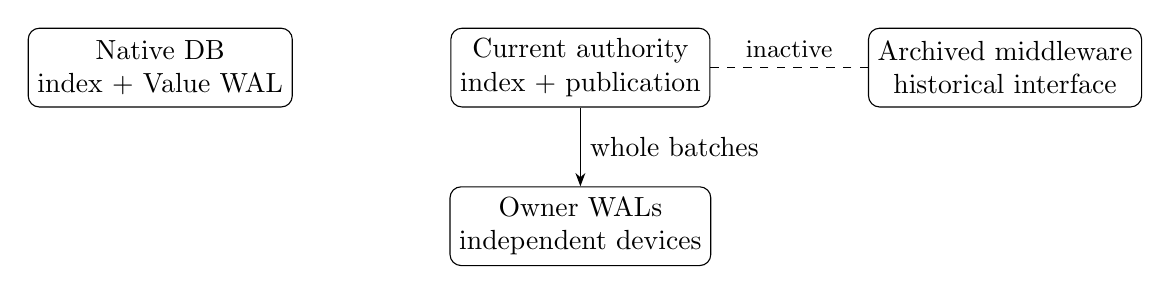
\begin{tikzpicture}[node distance=10mm, box/.style={draw,rounded corners,align=center,minimum height=10mm,minimum width=30mm}, >=Stealth]
\node[box] (n) {Native DB\\index + Value WAL};
\node[box,right=20mm of n] (a) {Current authority\\index + publication};
\node[box,below=of a] (o) {Owner WALs\\independent devices};
\node[box,right=20mm of a] (m) {Archived middleware\\historical interface};
\draw[->] (a)--node[right]{whole batches} (o);
\draw[dashed] (m)--node[above,font=\small]{inactive} (a);
\end{tikzpicture}
\caption{Three distinct implementation contexts. The current authority uses owner WAL machinery; archive middleware is not an active runtime dependency.}\label{fig:contexts}
\end{figure}

\subsection{Native DB, index and WAL in detail}\label{sec:native-detail}
The native design replaces an LSM value-compaction path with a Value WAL that is both recovery record and long-term value storage. A logical keyspace is divided into cells, each with independently managed index state. The Large Table locates keys and their WAL positions; its in-memory state, persisted cell indexes in the Index Store, and optional value cache serve different purposes. A Bloom filter can reject an absent key before a more expensive index lookup. A positive lookup still has to resolve a position and retrieve the value; a kernel page-cache hit is not a device read \cite{tidehunter2026}.

Cells can be fully resident, unloaded, or dirty while their old persisted index remains available. The dirty-unloaded approach buffers new entries without first loading a large cold cell. A background flusher captures dirty state, constructs or merges an index image and appends it to the Index Store. During construction readers continue to use the prior image; only after persistence does the cell point to its replacement. The exact state-machine and concurrency details are implementation-specific; the conceptual distinction is between a pending mutable overlay, the previously adopted image, and a newly persisted image.

For a uniformly distributed $b$-bit key $k$ and $N$ sorted keys, the paper's approximate expected rank is $Nk/2^b$. Here $k$ is interpreted as an integer in $[0,2^b)$ and rank is in entries, not bytes. This estimate is a search starting point, not a correctness oracle: the optimistic index checks the window bounds and shifts its search if required. Skew, sparse cells and cache or I/O behavior can change actual performance. The paper's illustration uses 256-bit keys and a default 800-entry window; neither number establishes a bound for this campaign's complete API latency. The header-based alternative uses a directory to select a region rather than predicting rank \cite{tidehunter2026}.

The native WAL controller allocates space, copies entries into mapped segments, tracks completion, maps new segments and asynchronously syncs finalized data. A higher native WAL position decides the later update of a key. A batch marker and single allocation support all-or-none recovery of a batch; individual index application steps must not be mistaken for a proof of general multi-database transactions. Snapshots record persisted cell-index locations and replay positions, so restart can reconstruct from a bounded WAL suffix rather than always starting at the beginning. Background relocation checks whether an old value is still live before re-appending it and changing its index reference; newer versions must not be replaced by an obsolete relocation. This is a native facility, not evidence that the distributed fork implements live-value relocation.

The native paper describes atomic allocation and concurrent work in components, but also fixed background workers and guard-protected state. Neither the native paper's component-level concurrency nor the fork's owner parallelism establishes that every operation in the distributed service is lock-free. Native ordinary page-cache completion is also distinct from stable-storage synchronization and from an explicit write barrier.


\section{Topology and implementation map}\label{sec:topology}
The measured implementation is source-pinned \cite{measuredcode2026}. The main implementation resides under \path{tidehunter/src/distributed/}, including authority sequencing, worker dispatch, publication, reference directory, owner storage, transport and checkpoint lifecycle. The fork retains the native engine under \texttt{tidehunter/src/}; \path{tidehunter-fabric/} provides fabric support. The comparison harness is in \path{experiments/kv-comparison/} and \path{benchmarks/kv-research/}. The archived \texttt{middleware-legacy} and \texttt{middleware-fabric-candidate} trees are historical, not active build or runtime dependencies. The legacy archive includes direct, primary-A, primary-B, Chord, XOR and hybrid experiments over native shard instances; the fabric candidate also explored coordinator/journal and participant commit machinery. Its Chord/XOR direct-owner approaches are not the original June option C broadcast design, and their routing or transactional properties must not be attributed to the current fork. The real Sui adapter is \texttt{distributed::sui::Db}: feature-gated typed-store integration maps exact canonical database paths to configured remote namespaces; missing mappings fail closed. One authority belongs to each logical database, not automatically to all of Sui's databases or keyspaces. The inspected Sui checkout at 2fc8fa1eb529cdeaa8cf3906c46d0de5e0b32a19 pins Tidehunter revision 9076518c\allowbreak b9e166e4\allowbreak 1b382d41\allowbreak bcc644db\allowbreak 94aa332b, not the measured ba3a6a0. Historical checkpoint/perpetual/current-epoch namespaces are a selected replay scope, not every Sui database. Hash keyspaces support full reduced-order enumeration, not application-key bounded range scans. The Sui native control has sharded-WAL selection disabled and rejects remote configuration; native Tidehunter itself remains enabled.

\begin{figure}[htbp]\centering
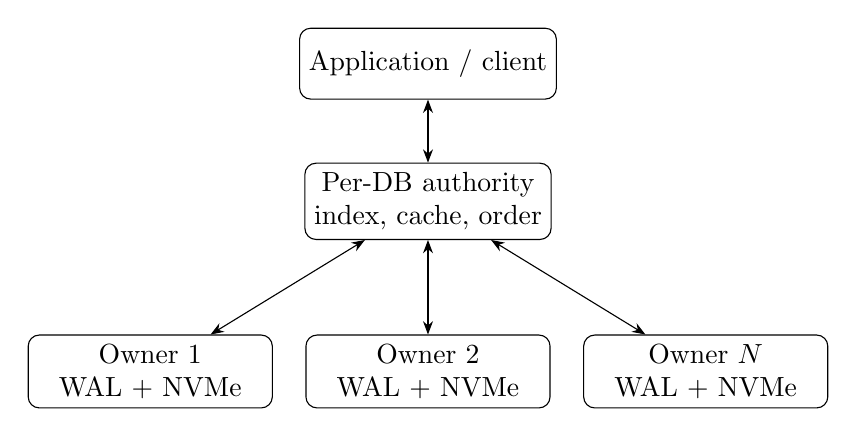
\begin{tikzpicture}[node distance=8mm, box/.style={draw,rounded corners,align=center,minimum width=31mm,minimum height=9mm}, >=Stealth]
\node[box] (c) {Application / client};
\node[box,below=of c] (a) {Per-DB authority\\index, cache, order};
\node[box,below left=12mm and 4mm of a] (o1) {Owner 1\\WAL + NVMe};
\node[box,below=12mm of a] (o2) {Owner 2\\WAL + NVMe};
\node[box,below right=12mm and 4mm of a] (o3) {Owner $N$\\WAL + NVMe};
\draw[<->] (c)--(a); \draw[<->] (a)--(o1); \draw[<->] (a)--(o2); \draw[<->] (a)--(o3);
\end{tikzpicture}
\caption{Logical topology; the measured fleet had five storage hosts and one controller. Lines represent transport interaction, not replication.}\label{fig:topology}
\end{figure}

\section{Write, visibility and read paths}\label{sec:paths}
\subsection{Logical ordering is not a global physical WAL}
The authority assigns an operation identity and logical batch version. Each owner allocates its own local physical WAL locations; there is no shared network fetch-and-add and no single global physical WAL offset. The complete atomic batch is sent to one selected owner, persisted there and acknowledged by a durable receipt; the authority publishes exact physical references in its index. Transport aggregation may combine complete batches, but must not split one batch across owners. Multiple owners and bounded preparation/append/persistence work permit overlap; shared authority state, index guards and native locks remain. No global lock-free claim follows.

\subsection{Record identity and address example}\label{sec:record-example}
The following example illustrates the types, not measured bytes or a real checkpoint. Let operation identity $B=(D,O)$ consist of a database ID $D$ and original operation ID $O$. Suppose the authority assigns batch version $(e,s)=(7,42)$ and the second member has operation index $1$: its mutation version is $(7,42,1)$. One possible owner frame location is $(p,g,o,\ell)=(3,12,4096,8192)$, meaning partition 3, segment generation 12, byte offset 4096 and frame length 8192. The figures are illustrative only; physical offsets in partition 3 are not comparable to offsets in another partition. A member descriptor then identifies its offset and length within that batch, keyspace, record kind, key and value bounds, operation index and checksum. The exact reference also carries the batch identity, logical version and batch digest. See \href{https://github.com/Loris-EPFL/tidehunter-distributed/blob/ba3a6a0194cca6f171e5916649e7f4eeba65aeb0/tidehunter/src/distributed/types.rs\#L8-L103}{the pinned type definitions}.

A new fenced writer epoch authorizes current requests; it is not a replacement for the original mutation version or retry identity. Frame generation guards against confusing a reused physical location with an earlier segment. The batch digest binds canonical contents and identity, and member CRC detects accidental corruption; neither authenticates a peer. A self-consistent member is not alone evidence that it belongs to a durable authorized batch. Owner membership and bounds, authority state and relevant read pins remain necessary.

\subsection{Ownership, worker and admission sequence}\label{sec:worker-flow}
At the coordinator, the write-owner command path owns mutable admission, dependency and publication decisions. The index and retention guards protect shared state and atomic views; the read service is separately accessible so that a remote wait need not occupy a serving index guard. Each partition owner has native WAL writer state, reference-directory metadata, synchronization and read-admission controls. Background metadata maintenance captures a durable complete-group prefix, writes metadata outside the foreground state lock, and adopts a durable replacement root before covered witnesses can be retired. The old root and charged pending suffix remain necessary until adoption. This is not a second value copy or LSM compaction.

\begin{enumerate}
\item The authority validates the operation, limits outstanding batches and bytes, determines reduced-key predecessor dependencies and preflights sparse-view capacity. The reservation precedes sequence allocation and owner WAL effects, so a quota rejection cannot be confused with an already durable write.
\item The authority assigns a logical batch version and selects one static owner by operation identity. Different batches may select different owners; a whole atomic batch is not split even when it modifies several keys. A later version of a key may select a different owner.
\item Bounded staging and transport group complete batches. On an owner, append execution and persistence may overlap with bounded work; the owner validates the frame and retry identity, appends the batch and persists the applicable WAL and namespace state before returning its durable receipt.
\item On receipt, the coordinator checks predecessor resolution. It publishes the complete batch under its index guard only when dependency-safe, then completes the caller. An unrelated earlier gap can remain; conflicting predecessors cannot be ignored. The stable prefix advances only over a contiguous resolved range.
\item A persistent gap holds bounded admission credits; later pressure eventually blocks or rejects admission rather than permitting unlimited suffix growth. An unknown append outcome or failed fence gates serving until recovery reconciles the inventory; an RPC timeout is not an abort certificate.
\end{enumerate}
Small staged owner tails can coalesce, whereas larger staged work may continue bounded pipelining. This is batch aggregation, not key-affinity placement, a new shared physical WAL, or weakened durability. Per-owner serialization and guards still exist. The source-level behavior is mapped in Appendix~\ref{app:source}; throughput and scheduling behavior depend on the actual workload and transport.

\subsection{Read and recovery algorithms}\label{sec:algorithm-detail}
A read first captures the appropriate index view and resolves a candidate exact reference. A verified coordinator-cache hit can return without owner traffic, but it does not bypass authority health. On a miss, references are grouped by owner and fetched by message or, when a valid immutable resident grant is available, through a registered-memory read. The owner checks complete-batch membership, address generation and bounds; the consumer validates identity, layout, key and checksum as applicable before returning bytes. A cache hit, grant or value reference is not independently a durable receipt or permission to reclaim its backing file. Multi-key reads retain a fixed cut across bounded windows and preserve caller ordering and per-key outcomes.

A stable checkpoint captures a contiguous published frontier and exact per-stream evidence while newer work may continue. It stages and persists the index image and manifest, adopts the replacement root and retains uncovered WAL history and pinned anchors. To recover, the coordinator establishes a new fenced authority, seals old streams, obtains available complete owner inventories, and merges actual complete batches by logical version. Duplicate or conflicting identity/version evidence is rejected; a retry is reconciled with retained evidence rather than treated as a fresh write merely because its earlier reply was lost. Recovery requires the relevant owner inventories and durable records: it is not a substitute for replication if the sole owner is permanently lost.

These mechanisms motivate limited invariant arguments, not a formal proof. Whole-batch owner append plus atomic coordinator index publication prevents this path from deliberately exposing only part of a batch. Dependency checks preserve the order of relevant predecessors while letting independent work progress. Stable-frontier checkpoints and retention pins prevent a sparse visible suffix from being mistaken for covered history. Fencing, inventory and retry identity address uncertain completion. Each argument assumes the corresponding checks, storage and owner evidence work as designed; it does not establish Byzantine safety, arbitrary-device-failure recovery or general serializability.


\subsection{Sparse live publication and stable prefixes}\label{sec:publication}
Dependency tracking uses native index identity, keyspace plus reduced key. Repeated keys, reduced-key collisions, deletes and transitive multi-key dependencies can therefore conflict. This reduction is lossy: distinct full keys that reduce to the same index slot are not merely delayed; a later key can make the earlier one absent in the exercised implementation. Hash keyspaces use a 16-byte digest. A durable batch may publish atomically and reply beyond a lower unresolved batch only when its actual predecessors have resolved. This provides dependency-aware progress, not a general serializability theorem. Genuine contiguous durable and published prefixes remain separate and protect stable checkpoint and recovery boundaries.

For example, suppose batch 1 is unresolved and batch 2 modifies a disjoint reduced key and is durable. Batch 2 may be live-visible while the stable contiguous prefix remains before batch 1. A later conflicting batch must respect its predecessors. A frozen index view records an upper mutation \emph{and exclusions}, with historical anchors pinned: merely retaining the upper number could admit a formerly excluded batch if it publishes later. View release releases retention charges. Admission reserves the possible sparse-view quota before sequence allocation and remote WAL effects; bounded windows and backpressure prevent unlimited growth behind a persistent hole. A held snapshot can cause a clean admission failure. These mechanisms are described in the 28 October update of the reference-directory design, not the obsolete contiguous-live-only brief.

\begin{figure}[htbp]\centering
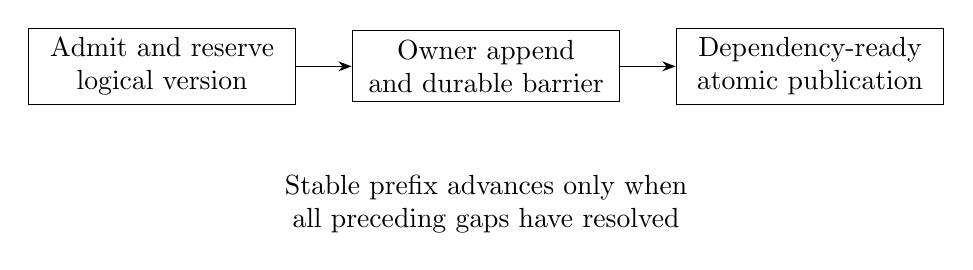
\begin{tikzpicture}[node distance=7mm, box/.style={draw,align=center,minimum width=34mm,minimum height=9mm}, >=Stealth]
\node[box] (a) {Admit and reserve\\logical version};
\node[box,right=of a] (w) {Owner append\\and durable barrier};
\node[box,right=of w] (p) {Dependency-ready\\atomic publication};
\draw[->] (a)--(w); \draw[->] (w)--(p);
\node[below=8mm of w,align=center] {Stable prefix advances only when\\all preceding gaps have resolved};
\end{tikzpicture}
\caption{The durable receipt is necessary but independent-key publication need not wait for an unrelated gap; stable checkpoint coverage remains contiguous.}\label{fig:write}
\end{figure}

\subsection{Reads, caching and grants}\label{sec:reads}
A read resolves an index reference at its view and can serve a verified coordinator-cache hit without remote data retrieval. On a miss the authority groups references by owner, requests values, and checks the returned data and current authority health. Owner-cache hits still pay remote interaction; OS page-cache residency is a distinct layer and logical WAL reads are not necessarily physical disk I/O. For eligible immutable registered resident data, a bounded grant can enable an actual libfabric \texttt{FI\_READ}; unregistered, unavailable or first-read cases use message fallback. The grant has lifetime, identity and integrity constraints and is not one-sided access to disk. The selected EFA-native transport label does not assert that all reads use RMA. No serving index or cache guard is held across a network wait.

\begin{figure}[htbp]\centering
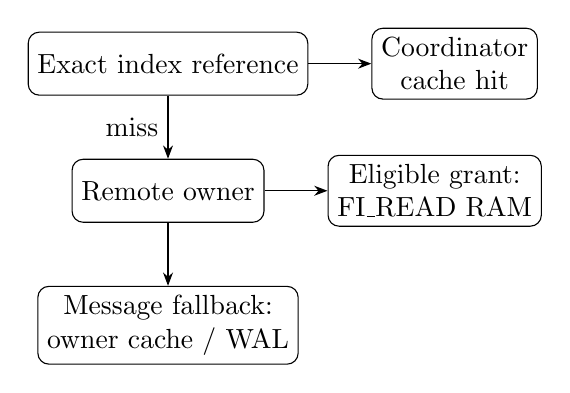
\begin{tikzpicture}[node distance=8mm, box/.style={draw,rounded corners,align=center,minimum height=8mm}, >=Stealth]
\node[box] (i) {Exact index reference};
\node[box,right=of i] (c) {Coordinator\\cache hit};
\node[box,below=of i] (r) {Remote owner};
\node[box,right=of r] (g) {Eligible grant:\\FI\_READ RAM};
\node[box,below=of r] (f) {Message fallback:\\owner cache / WAL};
\draw[->] (i)--(c); \draw[->] (i)--node[left]{miss} (r); \draw[->] (r)--(g); \draw[->] (r)--(f);
\end{tikzpicture}
\caption{Read tiers are distinct. Registered-memory access applies only to eligible resident values; fallback is retained.}\label{fig:read}
\end{figure}

\section{Maintenance, recovery and boundaries}\label{sec:recovery}
Background authority-history and checkpoint work is bounded and decoupled from append ownership. Checkpoints capture stable prefixes while live sparse suffixes and frozen-view anchors remain retained. Reopen fences old writers, seals streams, inventories owner batches and reconciles retry identities in logical version order. A timeout or unknown result is not automatically an abort: uncertain authority or fencing failure gates serving, including cached hits, until recovery reconciles outcomes. A later acknowledged batch cannot be discarded merely because an earlier unacknowledged sequence is absent. These are implementation mechanisms, not proof of resilience to arbitrary or Byzantine failures.

The sole RF1 owner's loss is not masked by replication. There is no consensus-backed membership, automatic failover or claim that distributed live values are relocated and packed as in native reclamation. Retention and no-physical-WAL-GC restrictions limit long-running operation. Tombstone-based adapter maintenance is not physical value-space reclamation. Pin-safe retirement of unreachable sealed files is distinct from distributed live-value relocation or packing. In the inspected Sui typed-store adapter, remote range tombstones are explicitly unsupported; the native Tidehunter branch falls through without scheduling one. Coordinator-only destruction, secondary mode, RocksDB range operations and directory-copy checkpoints are rejected where they cannot safely represent remote state. A frozen cut is an index-scoped snapshot mechanism, not a cross-database transaction.

\subsection{Live and stable views: an illustrative cut}
\begin{figure}[htbp]\centering
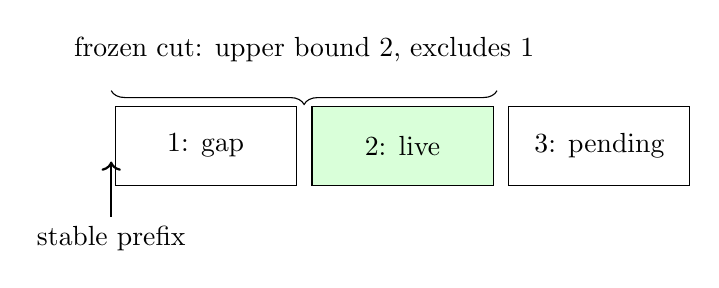
\begin{tikzpicture}[box/.style={draw,minimum width=23mm,minimum height=10mm,align=center}]
\node[box] (a) at (0,0) {1: gap}; \node[box,fill=green!15] (b) at (2.5,0) {2: live}; \node[box] (c) at (5,0) {3: pending};
\draw[thick,->] (-1.2,-0.9)--(-1.2,-0.2); \node[below] at (-1.2,-0.9) {stable prefix};
\draw[decorate,decoration={brace,amplitude=5pt}] (3.7,0.7)--(-1.2,0.7) node[midway,above=7pt] {frozen cut: upper bound 2, excludes 1};
\end{tikzpicture}
\caption{Illustrative independent batches: 2 may be published despite gap 1, but the stable prefix does not advance across 1. A frozen cut retains exclusions and their required history.}\label{fig:frontier}
\end{figure}
\subsection{Checkpoint and recovery lifecycle}
\begin{figure}[htbp]\centering
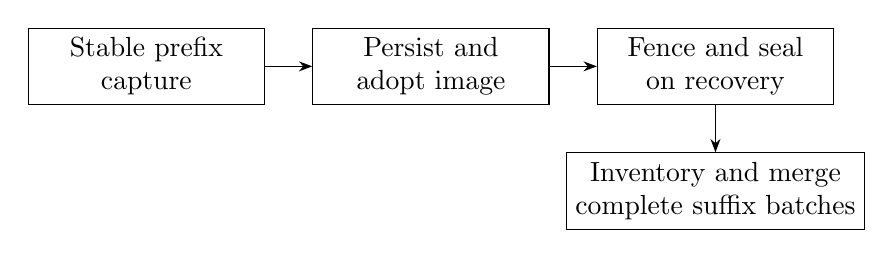
\begin{tikzpicture}[node distance=6mm, box/.style={draw,align=center,minimum height=9mm,minimum width=30mm}, >=Stealth]
\node[box] (s) {Stable prefix\\capture}; \node[box,right=of s] (d) {Persist and\\adopt image}; \node[box,right=of d] (f) {Fence and seal\\on recovery}; \node[box,below=of f] (r) {Inventory and merge\\complete suffix batches};
\draw[->] (s)--(d); \draw[->] (d)--(f); \draw[->] (f)--(r);
\end{tikzpicture}
\caption{Stable checkpoint coverage does not permit prematurely discarding live sparse suffixes or pinned history. Recovery reconciles uncertain operations after fencing.}\label{fig:lifecycle}
\end{figure}

\section{Comparison systems and experimental design}\label{sec:method}
The comparison includes native Tidehunter; TCP, EFA, EFA-direct and EFA-native distributed transports; TiKV, Cassandra, FoundationDB and Valkey TCP. The retained deployment pins TiKV/PD 8.5.4, Cassandra 5.0.9, FoundationDB 7.3.77 and Valkey 9.0.7; these versions identify the tested implementations rather than implying equivalent settings. Their reference designs differ: TiKV uses a transactional distributed KV architecture, Cassandra partitions data with tunable replication and consistency, FoundationDB offers transactional storage, and Valkey is an in-memory data structure server with selectable persistence. These reference capabilities do not imply that this RF1 experiment deployed their usual replicated or fault-tolerant production configurations. Transport selections change protocol paths, not replication factor. Mutual-TLS and trusted OFI are not security-equivalent: trusted OFI provides no application-level authentication or encryption. CRC verifies accidental corruption, not authenticity. Observed primary metadata reports mutual TLS for TCP, EFA and EFA-direct, but trusted direct OFI without TLS for EFA-native; thus their timing includes different security contracts. Cassandra and TiKV adapter metadata reports plaintext client transport, while FoundationDB effective TLS/authentication was not reported. Do not infer equivalence from the backend label. Per-case observed configuration is preserved in the data and Table~\ref{data-backend-contracts}; unavailable settings are unknown, not assumed equal. Persistence, atomic-batch behavior, security and consistency differ. For external design details see \cite{tikvstorage,cassandraengine,fdbarchitecture,valkeypersistence}.

The campaign used six On-Demand \texttt{g6.8xlarge} instances in \texttt{us-east-1a}, cluster placement, controller plus five storage hosts, and instance-store devices per owner. The configured server and client process caps were 8 vCPU and 16 GiB each; these per-process caps do not equalize aggregate cluster resources across deployments. Physical-host exclusivity was not established. The seven cohorts are primary (216 cases), cold OS cache (9), coordinator cache configured (8), owner cache configured (8), registered RAM configured (2), native page cache (10), and write-stage diagnostics (5). The case matrix in Table~\ref{data-matrix} is authoritative: coverage is not a Cartesian product of all operations, values and backends.

There is one independent repetition per case. Within-case standard deviation describes request samples, not run-to-run variation; no confidence interval or significance is inferred. Producer percentiles are retained unchanged: for $n$ ordered samples and percentile fraction $q$, the nearest-rank observation has one-based rank $\lceil qn\rceil$. p99 below 10,000 observations and p99.9 below 100,000 are descriptive tail estimates. Do not pool distinct operation, outcome, concurrency, cache or acknowledgment populations. Let $t_s$, $t_d$, and $t_c$ denote the client monotonic scheduled-arrival, observed backend dispatch, and materialized-response completion timestamps. For a dispatched call, the harness defines $T_{\rm sched}=t_d-t_s$, $T_{\rm API}=t_c-t_d$, and $T_{\rm response}=t_c-t_s$; byte verification occurs outside the API timer. Thus these durations add for the same observed call, but their separately computed quantiles cannot be added or subtracted to derive a percentile, one-way network duration or stage latency. Undispatched rejections have response observations but no invented dispatch, scheduling or API observations. The case and population appendices give counts, all available statistics, throughput and outcomes without replacing missing observations by zero.

\subsection{Reference design versus deployed adapter}
TiKV's reference design partitions key ranges into Regions and uses Raft groups with placement managed by PD; the evaluated RawKV adapter provides single-key semantics, not transactional batch writes. This deployment used one voter per Region, one PD and five stores, not the usual multi-replica availability configuration \cite{tikvstorage,tikvwrite854}. Cassandra's reference engine combines commitlog and memtable writes with SSTable flush and compaction; configurable consistency should not be confused with serializable cross-partition transactions. Here RF1 SimpleStrategy with QUORUM requires only one replica \cite{cassandraengine,cassandraconfig509}.

FoundationDB's reference design uses read versions, transaction conflict resolution, commit versions and transaction logs; this campaign used a single-replica configuration with one log and configured proxy/resolver counts, not replicated HA. Its transactional get-many behavior is not the same operation implementation as scalar fanout or grouped WAL reads \cite{fdbarchitecture,fdbconfig7377}. Valkey stores the active dataset in memory and distributes keys across hash slots; the campaign used five primaries without replicas and AOF \texttt{appendfsync=always}. Pipelining and client grouping reduce overhead but do not by themselves confer atomicity \cite{valkeycluster,valkeypersistence,valkeypipeline}. These version-specific deployment facts and uncertainties are recorded in \texttt{data/backend-contracts.json}; no power-failure experiment established identical durability.

The EFA provider and direct path differ in supported provider features; neither a provider label nor a requested mode proves that each operation was a native one-sided read \cite{awsefa,libfabricefa}. eRPC and FaRM illustrate transport and registered-memory design questions, but their in-memory results are not comparable to our end-to-end durable NVMe-backed workload \cite{erpc2019,farm2014}. WiscKey's key/value separation and Scalog's replicated shared ordering are useful conceptual contrasts, not evidence that this RF1 implementation adopts their mechanisms or guarantees \cite{wisckey2016,scalog2020}.

\subsection{TiKV: range regions, Raft and RawKV}
In the reference architecture, key ranges form Regions; Region replicas participate in Raft, and placement/control services maintain the cluster. A storage node applies committed changes to its local engine; the local LSM organizes mutable data and immutable files, with background compaction. The separation between Region-level replicated ordering and local storage is important: a collection of hosts is not by itself evidence of multiple copies of a given key. The benchmark uses the RawKV interface rather than TiKV's transactional API, and its configured Regions have one voter. The reported single-key operations and non-atomic batch behavior should not be described as a distributed transaction or multi-replica availability result \cite{tikvstorage,tikvwrite854}.

\subsection{Cassandra: partitioned log and LSM}
Cassandra's reference write flow routes by partition key to the selected replicas; each node records a mutation in its commitlog and updates a memtable, which is later flushed to immutable SSTables and compacted. Read and write consistency levels determine how many replica responses satisfy an operation, relative to its configured replication. In this campaign the observed keyspace is RF1: QUORUM therefore requires one replica, not a geographically resilient quorum. Its bounded per-key query fanout for get-many is not the same request as a single native batch read. The observed \texttt{durable\_writes} setting is recorded, while physical-device fsync behavior is not independently verified by this campaign \cite{cassandraengine,cassandraconfig509}.

\subsection{FoundationDB: transactional ordering and conflict checks}
FoundationDB's reference flow separates read-version acquisition, storage reads, commit ordering, conflict-range checking and transaction-log persistence. Its ordered transactional interface provides semantics that cannot be inferred merely from the same replica count as a RawKV or Tidehunter call. The measured adapter's get-many uses one transaction with sequential native gets and preserves caller order. The deployed \texttt{single} configuration and single log are RF1, not evidence of fault-tolerant replication; the documentation's conceptual architecture is not a version-specific proof of this campaign's storage engine or physical fsync behavior \cite{fdbarchitecture,fdbconfig7377}.

\subsection{Valkey: in-memory keyspace and append-only persistence}
Valkey's active dataset is memory-resident. Cluster slots distribute keys across primaries; a request to the client can be split across slots and reassembled in input order. Its append-only file is a persistence path, not the backing store for ordinary GETs. This campaign used five primaries, no replicas and observed AOF \texttt{appendfsync=always}; a successful SET acknowledgement is not a replica acknowledgement. The adapter's get-many uses a redis-rs MGET request with cross-slot splitting and ordered reassembly; a pipeline or a split read is not an atomic multi-key write. OS cache eviction does not evict the active RAM dataset \cite{valkeycluster,valkeypersistence,valkeypipeline}.

\begin{table}[htbp]\centering\small
\begin{tabular}{p{2.2cm}p{3.7cm}p{3.9cm}p{3.5cm}}\toprule
System & Principal reference design & Measured path & Important restriction\\\midrule
Native & Cell index and Value WAL & Embedded DB, explicit barrier & Same fork; no network\\
Distributed & Authority references, owner WALs & One owner per complete batch & RF1, no failover\\
TiKV & Region/Raft and local engine & RawKV, one Region voter & No transactional batch claim\\
Cassandra & Partition replicas, commitlog and SSTables & RF1, QUORUM, query fanout & One replica satisfies quorum\\
FoundationDB & Transaction versions, conflict checks and logs & Single configuration, transactional gets & Not replicated HA\\
Valkey & Memory-resident slots and optional AOF & Five primaries, no replicas, AOF always & RAM reads; no replica ACK\\\bottomrule
\end{tabular}
\caption{Qualitative design and experiment comparison. Configuration is not a power-loss equivalence test; see Table~\ref{data-backend-contracts} for observed details and unknown settings.}\label{tab:architecture-comparison}\end{table}

\begin{figure}[htbp]\centering
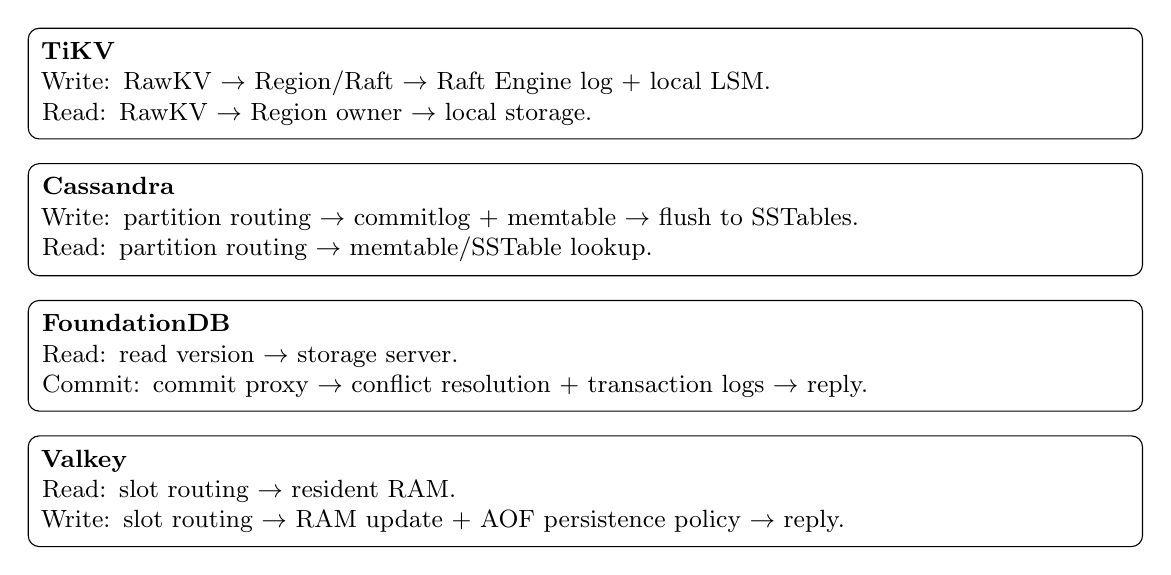
\begin{tikzpicture}[box/.style={draw,rounded corners,align=left,text width=13.8cm,inner sep=5pt,font=\small}]
\node[box] (tikv) {\textbf{TiKV}\\ Write: RawKV $\rightarrow$ Region/Raft $\rightarrow$ Raft Engine log + local LSM.\\ Read: RawKV $\rightarrow$ Region owner $\rightarrow$ local storage.};
\node[box,below=3mm of tikv] (cass) {\textbf{Cassandra}\\ Write: partition routing $\rightarrow$ commitlog + memtable $\rightarrow$ flush to SSTables.\\ Read: partition routing $\rightarrow$ memtable/SSTable lookup.};
\node[box,below=3mm of cass] (fdb) {\textbf{FoundationDB}\\ Read: read version $\rightarrow$ storage server.\\ Commit: commit proxy $\rightarrow$ conflict resolution + transaction logs $\rightarrow$ reply.};
\node[box,below=3mm of fdb] (valkey) {\textbf{Valkey}\\ Read: slot routing $\rightarrow$ resident RAM.\\ Write: slot routing $\rightarrow$ RAM update + AOF persistence policy $\rightarrow$ reply.};
\end{tikzpicture}
\caption{Coarse system-specific read and write paths, not a claim of equal semantics or physical fsync behavior. The tested deployments are RF1; FoundationDB reads and commit processing use distinct service paths. Refer to the system subsections and Table~\ref{data-backend-contracts} for adapter and configuration limits.}\label{fig:comparison-lens}\end{figure}


\section{Results and interpretation}\label{sec:results}
For the representative primary cases, uniform access over 4,096 keys at concurrency 16, the following table lists API p50/p99. Writes comprise 4,096 calls, scalar reads 8,192 and 32-key reads 2,048; selected calls succeeded. Batch latency is per batch, not per key. Explicit coordinator and owner value caches were disabled; Linux page cache remained available. Every p99 in this table is below the 10,000-call warning threshold.
\begin{table}[htbp]\centering\small
\begin{tabular}{lrrr}\toprule
Backend & 1 KiB write (ms) & 1 KiB read ($\mu$s) & 8 KiB $\times$ 32 read (ms)\\\midrule
Native & 0.702 / 3.311 & 1.920 / 3.500 & 0.134 / 0.260\\
TCP & 0.819 / 8.765 & 206.764 / 726.976 & 4.289 / 5.940\\
EFA & 0.683 / 14.881 & 120.153 / 398.000 & 3.780 / 5.521\\
EFA-direct & 0.676 / 14.437 & 120.972 / 399.139 & 4.183 / 6.244\\
EFA-native & 0.656 / 15.074 & 115.313 / 368.688 & 2.850 / 4.121\\
TiKV & 0.633 / 1.135 & 376.349 / 611.074 & 9.670 / 14.435\\
Cassandra & 0.510 / 1.705 & 235.405 / 349.348 & 4.575 / 17.434\\
FoundationDB & 0.964 / 1.564 & 592.943 / 844.498 & 14.174 / 17.760\\
Valkey TCP & 0.494 / 0.932 & 215.405 / 377.798 & 3.389 / 11.669\\\bottomrule
\end{tabular}
\caption{Selected API p50/p99, one repetition, different service contracts; source: retained campaign analysis.}\label{tab:representative}\end{table}

The 256-byte configured coordinator-cache EFA-native case at C1 had 8,192 hits, zero misses and zero remote RPCs, with 0.870/1.810 $\mu$s API p50/p99. This demonstrates a local hit path for that cohort, not remote access at that speed. Configured registered RAM at 256 B had 2,372 RMA completions and 5,820 message fallbacks; at 8 KiB, 2,361 and 5,831 respectively, each over 8,192 calls with zero recorded RMA errors. Aggregate p50/p99 of 54.001/473.281 and 60.762/500.741 $\mu$s respectively are mixed-path observations. OS-cache-drop is not a universal cold-physical-NVMe test: Valkey's RAM dataset and other user-space caches survive OS page-cache eviction.

All cases completed, but stress offered-load cases recorded 914,680 rejections at offered 50,000 and 74 at offered 10,000, total 914,754. No other non-success population was observed. Success-only latency must be read together with throughput and rejection counts. The earlier 27 October campaign used Frankfurt \texttt{eu-central-1c}; this one used \texttt{us-east-1a}, and source changed. In matched 1 KiB writes, TCP p99 changed 144.163 to 8.765 ms, EFA 142.793 to 14.881 ms, direct 142.884 to 14.437 ms, EFA-native 142.371 to 15.074 ms, native 3.318 to 3.311 ms. These single-run cross-region historical observations do not isolate a code change or establish statistical significance. Historical-only and current-only populations remain distinct.

\subsection{Representative empirical latency distributions}\label{sec:ecdf}
Figures~\ref{fig:ecdf-read} and \ref{fig:ecdf-put} show each backend's separate empirical API-latency distribution for the primary 1 KiB concurrency-16 read and write cases. Each curve is from one case and one repetition, not a pooled distribution. The read curves contain 8,192 successful dispatched measurement-phase calls per backend; the write curves contain 4,096. Explicit Tidehunter value caches are disabled, but operating-system page cache may be warm. Native and distributed acknowledgment and security contracts differ. Source filters and raw hashes are in \path{data/ecdf-source-hashes.json}; \path{data/ecdf-samples.csv} is the selected reproducible snapshot.
\begin{figure}[p]\centering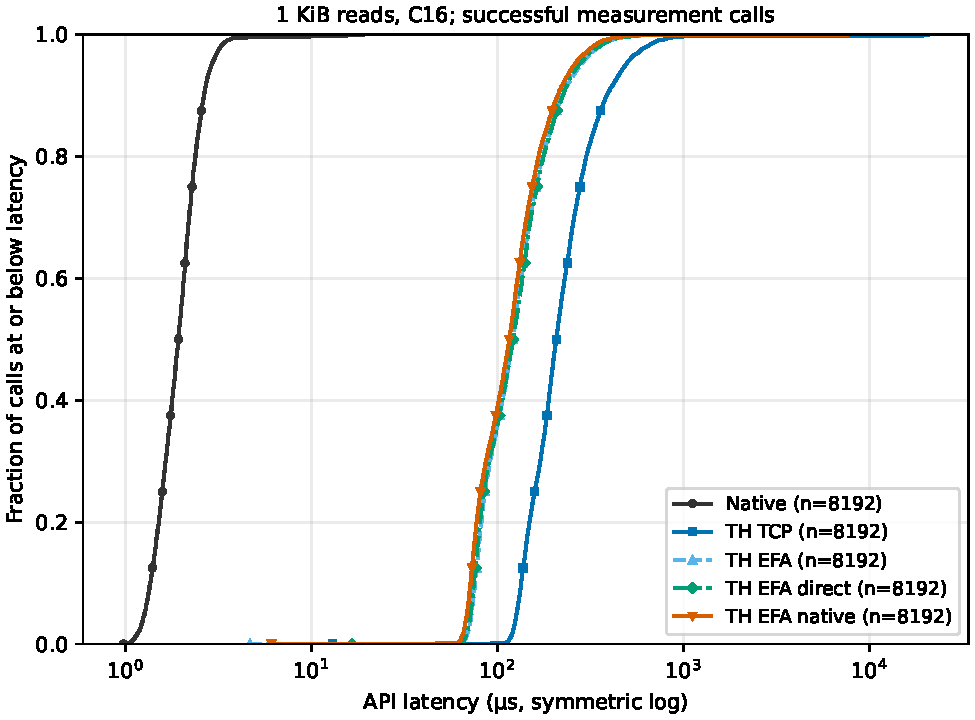
\includegraphics[width=\linewidth,height=.75\textheight,keepaspectratio]{figures/eval/ecdf-read-1k.pdf}\caption{Empirical API-latency CDF, primary 1 KiB C16 successful scalar reads, 8,192 calls per system; one independent repetition, no pooling. Warm OS cache is possible.}\label{fig:ecdf-read}\end{figure}
\begin{figure}[p]\centering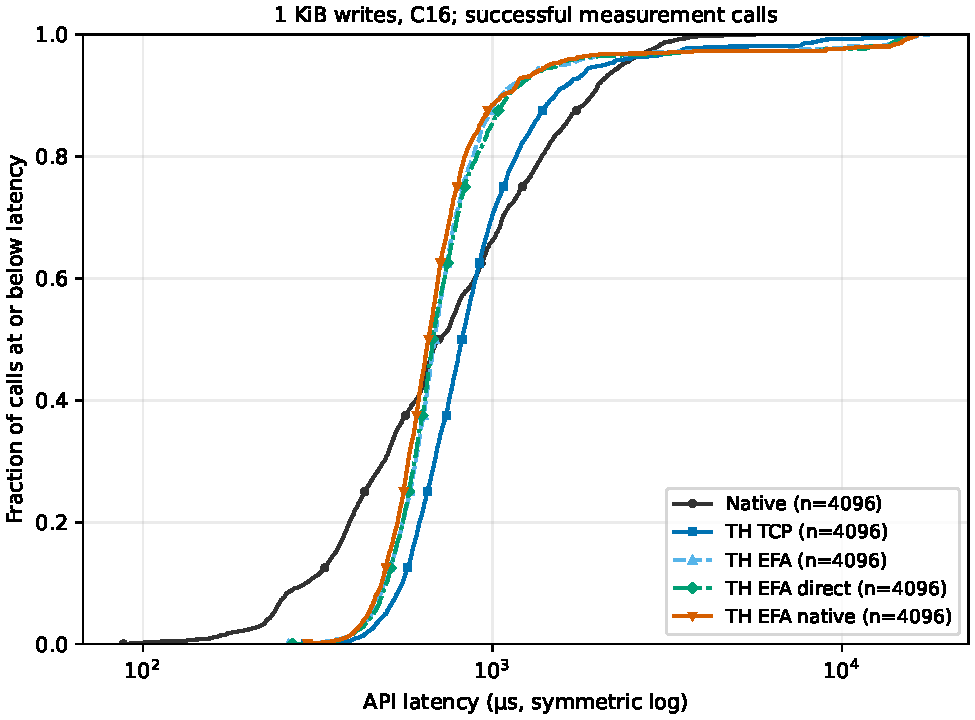
\includegraphics[width=\linewidth,height=.75\textheight,keepaspectratio]{figures/eval/ecdf-put-1k.pdf}\caption{Empirical API-latency CDF, primary 1 KiB C16 successful scalar writes, 4,096 calls per system; one independent repetition, no pooling. Durability and security contracts differ.}\label{fig:ecdf-put}\end{figure}

\section{Observability, cache provenance and bottleneck limits}\label{obs-observability}
The following observations concern the synthetic campaign, not Sui replay. Primary cases and the five separately executed 1,024-byte concurrent-write diagnostic cases are distinct populations. Each case has one repetition. The retained machine-readable \path{data/observability-evidence.json} includes exact case identifiers, raw stage counters, read-boundary deltas, host device and cgroup intervals, replay queries and units. Source is campaign 40848651463, at revision \texttt{ba3a6a0194cca6f171e5}\allowbreak\texttt{916649e7f4eeba65aeb0}. Stage definitions at that revision are in the following source files: \path{benchmarks/kv-research/src/backends/tidehunter.rs}; \path{tidehunter/src/distributed/tcp/diagnostics.rs}.

\subsection{Coverage and offline verification}\label{obs-coverage}
The monitoring capture reports 258 expected cases, 258 seen and 258 terminal observations, with no capture gaps under its own completeness criterion. It retained 378 query page receipts across 27 metric families, 339 unique page files, and a TSDB block with 4,508,934 samples and 195,976 series. Host and explicitly selected cgroup targets were scraped every 5 seconds, benchmark gauges every second. Initial verification reported 13 targets and 27 executable panels; the final Cassandra-anchored panels include empty queries. Missing data is not zero. The collector was cohosted and its overhead was not calibrated. Short cases and rolling rate windows need not align: host-wide CPU, memory, network, pressure and device signals include background and observation work. Selected cgroups are not a complete process-discovery or cross-backend cache-coverage guarantee.

Using the retained archive and already cached pinned images, an offline replay restored original timestamps; authenticated Grafana/datasource verification completed successfully and the replayed Prometheus host and resource queries returned data. Only the two owned replay containers were stopped afterwards. This was API/query verification, not visual inspection of Grafana. At Unix time 1793270529.054, near the capture end, all six host series reported swap total and swap free as zero, and the \texttt{nvme1n1} in-flight I/O gauge was zero at that instant. Host available memory was 119.77--121.00 billion bytes, and file-cache gauges were 0.359--1.558 billion bytes. These are host-level snapshots, not cgroup memory usage, peak disk queue depth during the cases, or evidence of absent stalls. A 20-second non-loopback receive-rate query returned points; it mixes host/background traffic and is not a per-case network accounting. ENA and Linux network-device counters can omit OS-bypass EFA traffic: absent or low counters do not establish an idle EFA NIC.

\subsection{What measured write stages can localize}\label{obs-stages}
Each distributed diagnostic captures the first 256 append requests on each of five append-owning connections after measurement arming: 1,280 selected requests, not a random sample and not the 4,096 logical writes in its coordinator interval. Client exchange, server handler, owner execution, persistence and transport clocks overlap or nest. Stage sums across requests and machines are not elapsed case time; queue residence through local completion is not peer receipt. The connection receive/idle field is not attributable under multiplexing and is retained as zero, not measured zero idle. The coordinator baseline is taken at arm time and the end before profile finalization. The following sums are descriptive diagnostic evidence in milliseconds; they are neither latency percentiles nor an additive critical-path decomposition.

\begin{center}\small
\begin{tabular}{lrrrrrr}
\hline
Diagnostic & Owner append & Append calls & Persist & Persist calls & WAL file & File calls\\
\hline
TCP & 156.319 & 1280 & 217.045 & 1280 & 165.336 & 1099\\
EFA & 120.249 & 1280 & 203.480 & 1280 & 165.815 & 1165\\
EFA direct & 110.205 & 1280 & 194.981 & 1280 & 163.056 & 1182\\
EFA native label & 117.908 & 1280 & 199.573 & 1280 & 165.096 & 1160\\
\hline
\end{tabular}
\end{center}
For example, the EFA-native diagnostic recorded 468.276 ms client exchange summed across 1,295 client requests, and 74.787 ms control-queue residence across 1,295 queue samples. These denominators differ from the 1,280 owner append calls and 1,160 file-persist calls, so dividing every clock by 1,280 or comparing the sums as disjoint components is invalid. Its coordinator interval records 4,096 admitted and completed writes, 2,207 append requests, 1,854 durable-receipt publication-blocked batches and one dependency-wait batch; these counters are not per-call tail attribution. The standalone native diagnostic selects the first 256 scalar writes: append sum 103.895 ms, index application 0.890 ms, and separately sampled WAL file persistence 176.219 ms across 512 file calls and namespace persistence 3.702 ms across 256 calls. Persistence components are nested in the foreground barrier, not extra stages to add to it. Batch native writes and per-operation stage percentiles are unsupported.

Current primary 1 KiB write p99 is 8.765 ms TCP, 14.881 ms EFA, 14.437 ms direct and 15.074 ms EFA-native, versus 3.311 ms native. Each write population has 4,096 calls, fewer than 10,000; its p99 is therefore flagged as sparsely supported and is not a run-to-run uncertainty estimate. Their historical counterparts were 144.163, 142.793, 142.884, 142.371 and 3.318 ms respectively. The older Frankfurt fleet and current Virginia fleet differ: this is descriptive, not a controlled code-only comparison. Current summed diagnostic clocks and interval counters show work in several stages but do not reveal which stage caused an individual primary p99, much less isolate the old tail. No one-way network duration follows from subtracting unsynchronized node clocks or from adding/subtracting independently computed quantiles.

\subsection{Read-path provenance and physical-I/O boundaries}\label{obs-cache}
The primary Tidehunter configuration disables explicit coordinator and owner value caches; it does not make the Linux page cache cold. In the EFA-native primary 1 KiB concurrent-read case, measurement-boundary deltas show 8,192 coordinator cache bypasses, 8,162 remote read RPCs and 8,162 logical owner WAL reads and async submissions. They do not all have a one-to-one relation to the 8,192 calls: coordinator misses total 15,516. Async submission and logical WAL read are not proof of physical-device access. Owner snapshots are sequential and not globally atomic.

Configured-cache cohorts are separate from primary. In case 0078 (EFA-native, 256 B, concurrency 1), the measurement boundary shows 8,192 coordinator-cache hits, zero misses and zero remote RPCs; API p50/p99 are 0.870/1.810 microseconds. This is a local cache-hit workload, not evidence of remote 1.810 microsecond p99 and not directly comparable to native at concurrency 16. In all eight owner-cache cases (256 B and 8 KiB across four transports), 8,192 owner lookups comprise 5,435 owner-cache hits and 2,757 misses/logical WAL reads. This explicit owner value cache is different from the Linux resident-WAL/NOWAIT path and from the kernel page cache. The 8 KiB TCP coordinator-cache case has 8,188 hits and four misses/RPCs; the other seven coordinator-cache cases have 8,192 hits and zero misses/RPCs.

Registered-RAM EFA-native cases are mixed populations: the 256 B case has 2,372 RMA hits/completions and 5,820 message requests, and the 8 KiB case 2,361 and 5,831 respectively, each out of 8,192, with zero RMA errors. The corresponding owner snapshots also report 5,820 and 5,831 successful resident reads. Thus roughly 29\% of calls used RMA in these cases; aggregate latency is not pure RMA latency. The EFA-native label does not imply all primary reads are one-sided.

All nine 64 KiB cold-OS-cache cases record a requested OS cache drop on all six hosts but \texttt{application\_\allowbreak caches\_\allowbreak evicted=false}; this cannot evict all database caches. The whole-host instance-store device read deltas support physical activity during boundaries, not attribution to individual GETs. For example EFA-native storage-0 reports 139,856 sectors, or 71,606,272 bytes, while its selected storage cgroup reports 70,995,968 read bytes; native's coordinator reports 546,104 sectors, or 279,605,248 bytes. These scopes and sampling boundaries differ. Valkey's dataset remains RAM-resident despite host I/O; FoundationDB, TiKV and Cassandra may retain their own caches. No common nine-backend hit ratio or universal per-request physical-NVMe claim is established.

\subsection{Resource signals and cautious interpretation}\label{obs-resource}
Matched primary 1 KiB concurrent reads show EFA-native storage-0 using 6.302326 CPU seconds over 1.556699393 seconds, about 4.049 average cores, and zero observed throttled periods in that selected cgroup interval; its other four storage roles average 4.046--4.052 cores. The TCP storage roles average 0.126--0.135 cores in their own intervals. EFA-native's client reports one throttled period of nine, with 0.022251 seconds throttled; the selected storage cgroups report no throttled periods. These intervals include gating/control and background activity and are not CPU per operation, instantaneous saturation, or proof that polling caused a latency difference. All selected EFA-native storage cgroups report zero read bytes in that warm boundary interval; that cgroup accounting does not prove every read was cached or identify physical reads outside its scope. Cgroup memory current is an end-boundary gauge, while memory peak is a cgroup-lifetime high-water mark, not interval RSS. Workload ceilings were 8 vCPU and 16 GiB per server/client host, with role-specific allocations possible.

The read-path deltas, CPU contrast, persistence and queue sums provide hypotheses for targeted instrumentation; none independently establishes a causal bottleneck. Additional independent repetitions, correlated per-request spans with synchronized clocks, verified EFA provider/NIC counters, physical-I/O attribution and calibrated observer overhead would be needed to localize tails more confidently.

\section{Cost, provenance and closure}\label{sec:provenance}
The retained model reports partial observed-resource estimates, not bills: run/day USD 15.732270682006, calendar week 39.432293945896, and October/tracked lifetime since 18 October 210.356778876398. The rolling budget charge was 187.248684844483 against a USD 230 cap, leaving 42.751315155517; active holds were zero. These overlapping scopes are not additive. Official tag-attributed billing was unavailable because \texttt{ListCostAllocationTags} was denied; this is not evidence of zero charge. Retained shared evidence and control infrastructure may incur costs.

The source-bound campaign had 258 completed cases and complete monitoring. All six instances were observed terminated by 10:51:35 UTC; independent inventories across five approved regions at 11:13:16--11:13:45 found no run-owned active fleet resources, and run roles/profiles were absent at 11:07. Artifact retrieval verified 5,865 files and three GitHub ZIP digests. The comparison JSON SHA-256 is \texttt{aa6a0d32a999d2dd\allowbreak 1c1a38cc4573c046\allowbreak 4a038ec9603a56e4\allowbreak 672107e5d03cdfde}. Raw CSV samples, machine-readable configurations, observability receipts, accounting, validation and resource journals reside in the retained run directory; they are not reproduced as independent experiments here.

\section{Limitations and next research questions}\label{sec:limitations}
Current evidence does not establish failover, replicated durability, a globally lock-free service, universal cold-device speed, pure one-sided latency, production security equivalence, distributed physical relocation, or Sui performance for this latest synthetic campaign. The earlier real checkpoint studies are separate workloads and revisions. Open questions include repeated same-region matched experiments with controlled acknowledgment tiers, per-path cache and actual device-I/O attribution, scaling of a bounded single authority and retained history, resource and memory pressure under stalled holes, distributed value reclamation, and explicit replicated recovery/failure semantics. Any future experiment must retain offered-load outcomes and separate cold/warm/cache populations. External RAM microbenchmarks are not substitutes for these NVMe-backed end-to-end results.

\appendix
\section{Evaluation figures}\label{app:figures}
Figures use retained single-run measurements, no run-to-run uncertainty bars. Consult Tables~\ref{data-cases} and \ref{data-latencies} for exact populations, sample counts and all clocks; p99 below 10,000 and p99.9 below 100,000 calls are descriptive. Guarantees differ across systems.
\begin{figure}[p]\centering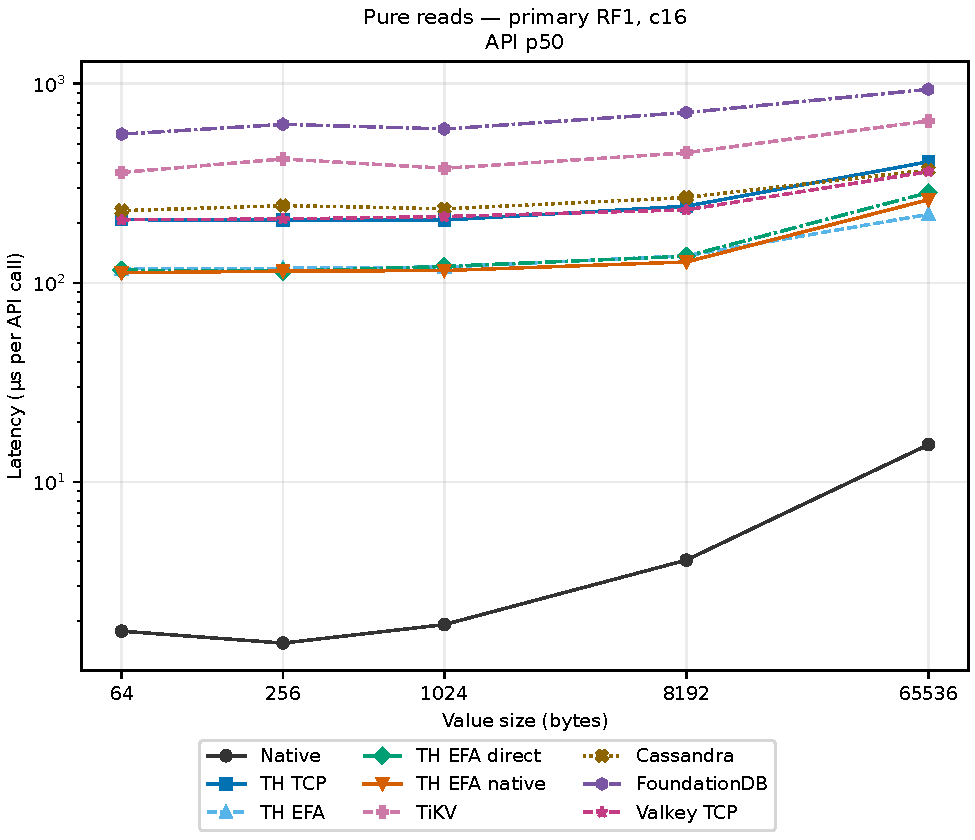
\includegraphics[page=1,width=\linewidth,height=.75\textheight,keepaspectratio]{figures/eval/panels/primary-read-concurrent.pdf}\caption{API p50. Primary concurrent scalar reads; latency comparisons are API populations with warm operating-system cache possible. One independent repetition per case; units and workload dimensions are shown in the plot.}\label{fig:eval-primary-read-concurrent-1}\end{figure}
\begin{figure}[p]\centering\includegraphics[page=2,width=\linewidth,height=.75\textheight,keepaspectratio]{figures/eval/panels/primary-read-concurrent.pdf}\caption{API p99. Primary concurrent scalar reads; latency comparisons are API populations with warm operating-system cache possible. One independent repetition per case; units and workload dimensions are shown in the plot.}\label{fig:eval-primary-read-concurrent-2}\end{figure}
\begin{figure}[p]\centering\includegraphics[page=3,width=\linewidth,height=.75\textheight,keepaspectratio]{figures/eval/panels/primary-read-concurrent.pdf}\caption{Response p99. Primary concurrent scalar reads; latency comparisons are API populations with warm operating-system cache possible. One independent repetition per case; units and workload dimensions are shown in the plot.}\label{fig:eval-primary-read-concurrent-3}\end{figure}
\begin{figure}[p]\centering\includegraphics[page=4,width=\linewidth,height=.75\textheight,keepaspectratio]{figures/eval/panels/primary-read-concurrent.pdf}\caption{Whole-workload successful calls. Primary concurrent scalar reads; latency comparisons are API populations with warm operating-system cache possible. One independent repetition per case; units and workload dimensions are shown in the plot.}\label{fig:eval-primary-read-concurrent-4}\end{figure}
\begin{figure}[p]\centering\includegraphics[page=5,width=\linewidth,height=.75\textheight,keepaspectratio]{figures/eval/panels/primary-read-concurrent.pdf}\caption{Successful logical keys. Primary concurrent scalar reads; latency comparisons are API populations with warm operating-system cache possible. One independent repetition per case; units and workload dimensions are shown in the plot.}\label{fig:eval-primary-read-concurrent-5}\end{figure}
\begin{figure}[p]\centering\includegraphics[page=6,width=\linewidth,height=.75\textheight,keepaspectratio]{figures/eval/panels/primary-read-concurrent.pdf}\caption{Successful value payload. Primary concurrent scalar reads; latency comparisons are API populations with warm operating-system cache possible. One independent repetition per case; units and workload dimensions are shown in the plot.}\label{fig:eval-primary-read-concurrent-6}\end{figure}
\begin{figure}[p]\centering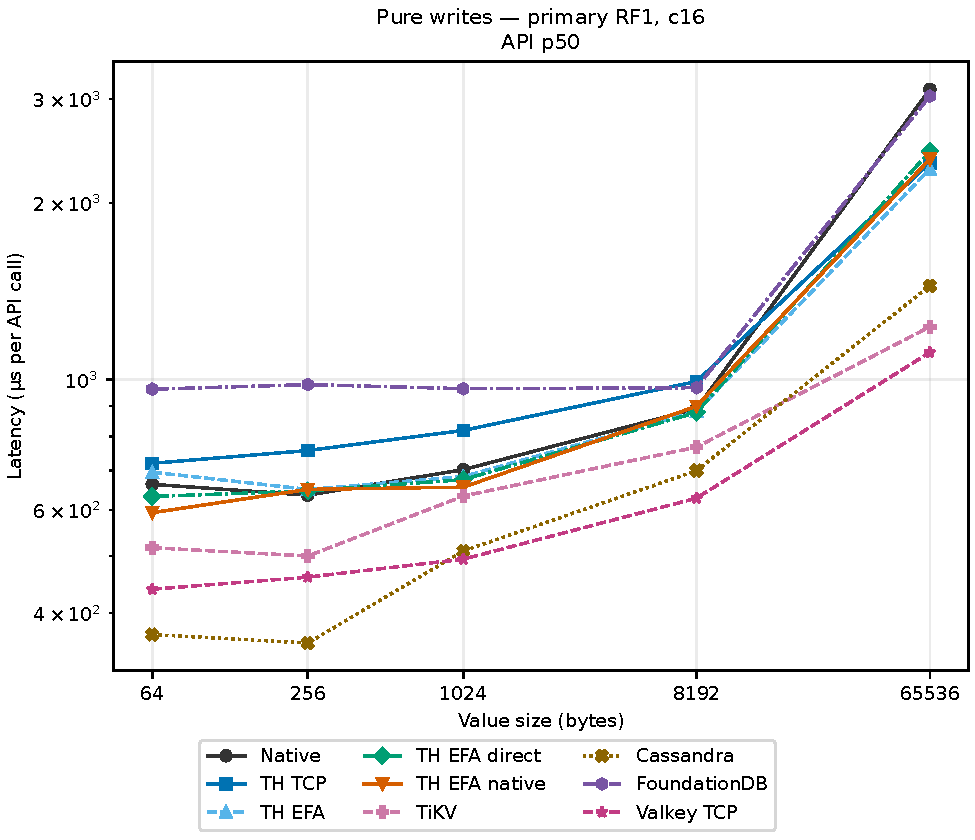
\includegraphics[page=1,width=\linewidth,height=.75\textheight,keepaspectratio]{figures/eval/panels/primary-write-concurrent.pdf}\caption{API p50. Primary concurrent scalar writes; native uses the explicit Value-WAL barrier. One independent repetition per case; units and workload dimensions are shown in the plot.}\label{fig:eval-primary-write-concurrent-1}\end{figure}
\begin{figure}[p]\centering\includegraphics[page=2,width=\linewidth,height=.75\textheight,keepaspectratio]{figures/eval/panels/primary-write-concurrent.pdf}\caption{API p99. Primary concurrent scalar writes; native uses the explicit Value-WAL barrier. One independent repetition per case; units and workload dimensions are shown in the plot.}\label{fig:eval-primary-write-concurrent-2}\end{figure}
\begin{figure}[p]\centering\includegraphics[page=3,width=\linewidth,height=.75\textheight,keepaspectratio]{figures/eval/panels/primary-write-concurrent.pdf}\caption{Response p99. Primary concurrent scalar writes; native uses the explicit Value-WAL barrier. One independent repetition per case; units and workload dimensions are shown in the plot.}\label{fig:eval-primary-write-concurrent-3}\end{figure}

\clearpage
\begin{figure}[p]\centering\includegraphics[page=4,width=\linewidth,height=.75\textheight,keepaspectratio]{figures/eval/panels/primary-write-concurrent.pdf}\caption{Whole-workload successful calls. Primary concurrent scalar writes; native uses the explicit Value-WAL barrier. One independent repetition per case; units and workload dimensions are shown in the plot.}\label{fig:eval-primary-write-concurrent-4}\end{figure}
\begin{figure}[p]\centering\includegraphics[page=5,width=\linewidth,height=.75\textheight,keepaspectratio]{figures/eval/panels/primary-write-concurrent.pdf}\caption{Successful logical keys. Primary concurrent scalar writes; native uses the explicit Value-WAL barrier. One independent repetition per case; units and workload dimensions are shown in the plot.}\label{fig:eval-primary-write-concurrent-5}\end{figure}
\begin{figure}[p]\centering\includegraphics[page=6,width=\linewidth,height=.75\textheight,keepaspectratio]{figures/eval/panels/primary-write-concurrent.pdf}\caption{Successful value payload. Primary concurrent scalar writes; native uses the explicit Value-WAL barrier. One independent repetition per case; units and workload dimensions are shown in the plot.}\label{fig:eval-primary-write-concurrent-6}\end{figure}
\begin{figure}[p]\centering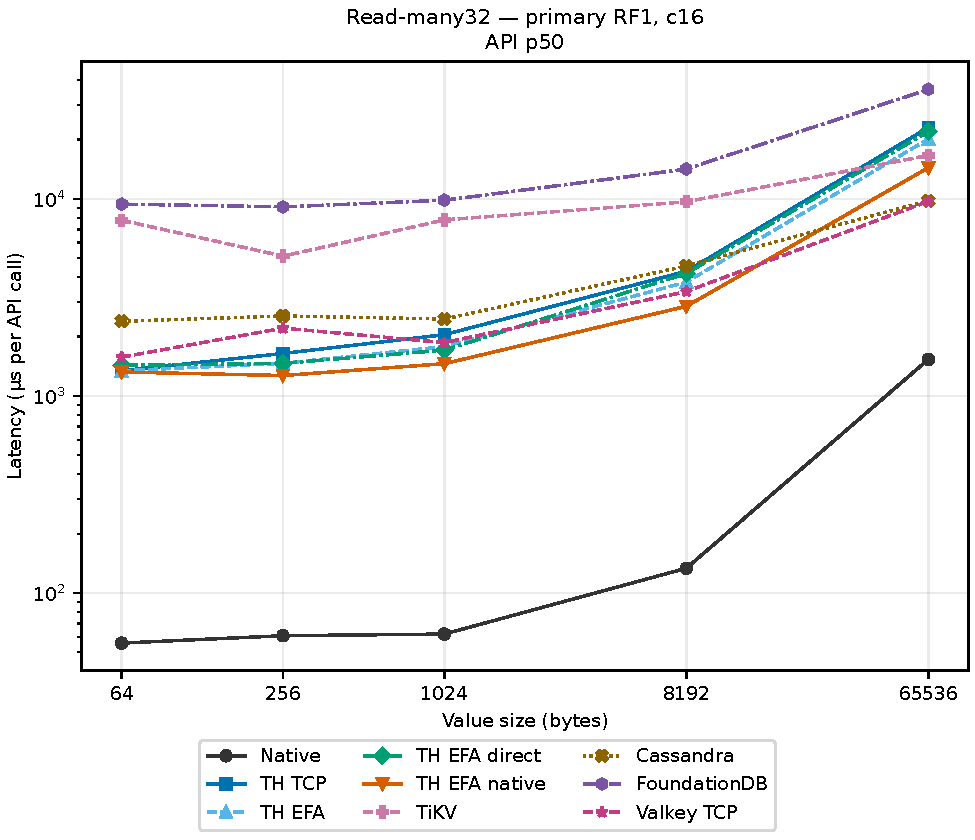
\includegraphics[page=1,width=\linewidth,height=.75\textheight,keepaspectratio]{figures/eval/panels/primary-read-many32.pdf}\caption{API p50. Primary 32-key read calls; batch latency is per call and adapters use different get-many implementations. One independent repetition per case; units and workload dimensions are shown in the plot.}\label{fig:eval-primary-read-many32-1}\end{figure}
\begin{figure}[p]\centering\includegraphics[page=2,width=\linewidth,height=.75\textheight,keepaspectratio]{figures/eval/panels/primary-read-many32.pdf}\caption{API p99. Primary 32-key read calls; batch latency is per call and adapters use different get-many implementations. One independent repetition per case; units and workload dimensions are shown in the plot.}\label{fig:eval-primary-read-many32-2}\end{figure}
\begin{figure}[p]\centering\includegraphics[page=3,width=\linewidth,height=.75\textheight,keepaspectratio]{figures/eval/panels/primary-read-many32.pdf}\caption{Response p99. Primary 32-key read calls; batch latency is per call and adapters use different get-many implementations. One independent repetition per case; units and workload dimensions are shown in the plot.}\label{fig:eval-primary-read-many32-3}\end{figure}
\begin{figure}[p]\centering\includegraphics[page=4,width=\linewidth,height=.75\textheight,keepaspectratio]{figures/eval/panels/primary-read-many32.pdf}\caption{Whole-workload successful calls. Primary 32-key read calls; batch latency is per call and adapters use different get-many implementations. One independent repetition per case; units and workload dimensions are shown in the plot.}\label{fig:eval-primary-read-many32-4}\end{figure}
\begin{figure}[p]\centering\includegraphics[page=5,width=\linewidth,height=.75\textheight,keepaspectratio]{figures/eval/panels/primary-read-many32.pdf}\caption{Successful logical keys. Primary 32-key read calls; batch latency is per call and adapters use different get-many implementations. One independent repetition per case; units and workload dimensions are shown in the plot.}\label{fig:eval-primary-read-many32-5}\end{figure}
\begin{figure}[p]\centering\includegraphics[page=6,width=\linewidth,height=.75\textheight,keepaspectratio]{figures/eval/panels/primary-read-many32.pdf}\caption{Successful value payload. Primary 32-key read calls; batch latency is per call and adapters use different get-many implementations. One independent repetition per case; units and workload dimensions are shown in the plot.}\label{fig:eval-primary-read-many32-6}\end{figure}
\begin{figure}[p]\centering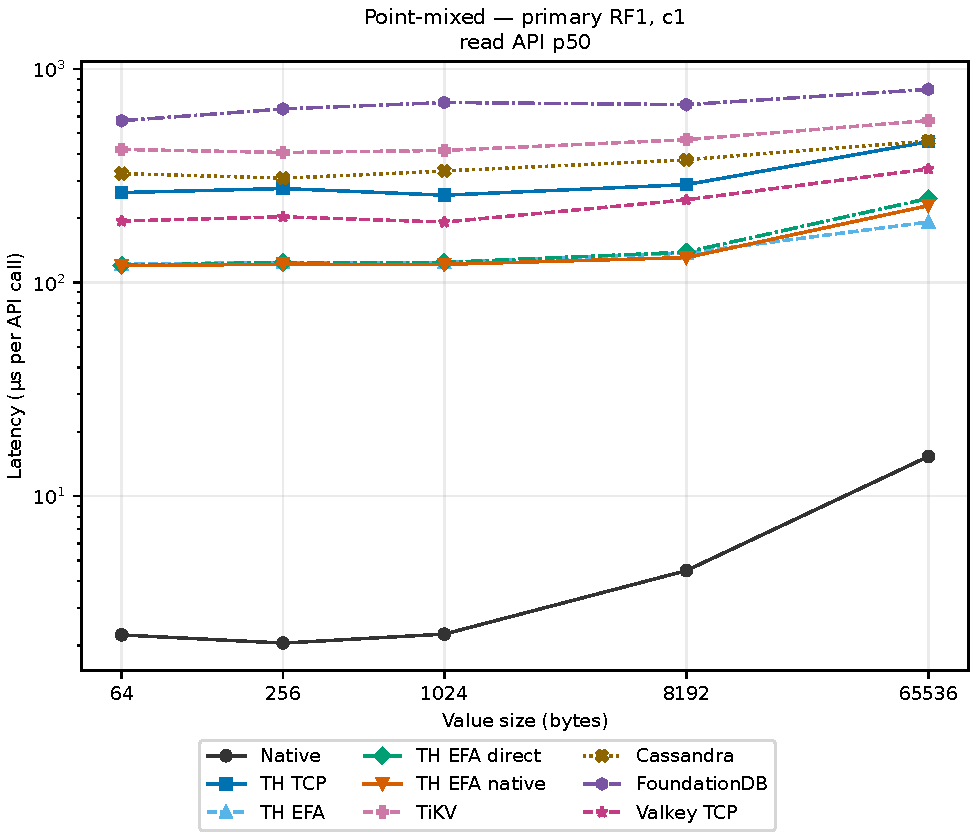
\includegraphics[page=1,width=\linewidth,height=.75\textheight,keepaspectratio]{figures/eval/panels/primary-point-mixed-latency.pdf}\caption{read API p50. Primary point-mixed latency, retaining separate operation populations. One independent repetition per case; units and workload dimensions are shown in the plot.}\label{fig:eval-primary-point-mixed-latency-1}\end{figure}

\clearpage
\begin{figure}[p]\centering\includegraphics[page=2,width=\linewidth,height=.75\textheight,keepaspectratio]{figures/eval/panels/primary-point-mixed-latency.pdf}\caption{put API p50. Primary point-mixed latency, retaining separate operation populations. One independent repetition per case; units and workload dimensions are shown in the plot.}\label{fig:eval-primary-point-mixed-latency-2}\end{figure}
\begin{figure}[p]\centering\includegraphics[page=3,width=\linewidth,height=.75\textheight,keepaspectratio]{figures/eval/panels/primary-point-mixed-latency.pdf}\caption{delete API p50. Primary point-mixed latency, retaining separate operation populations. One independent repetition per case; units and workload dimensions are shown in the plot.}\label{fig:eval-primary-point-mixed-latency-3}\end{figure}
\begin{figure}[p]\centering\includegraphics[page=4,width=\linewidth,height=.75\textheight,keepaspectratio]{figures/eval/panels/primary-point-mixed-latency.pdf}\caption{missing\_read API p50. Primary point-mixed latency, retaining separate operation populations. One independent repetition per case; units and workload dimensions are shown in the plot.}\label{fig:eval-primary-point-mixed-latency-4}\end{figure}
\begin{figure}[p]\centering\includegraphics[page=5,width=\linewidth,height=.75\textheight,keepaspectratio]{figures/eval/panels/primary-point-mixed-latency.pdf}\caption{read API p99. Primary point-mixed latency, retaining separate operation populations. One independent repetition per case; units and workload dimensions are shown in the plot.}\label{fig:eval-primary-point-mixed-latency-5}\end{figure}
\begin{figure}[p]\centering\includegraphics[page=6,width=\linewidth,height=.75\textheight,keepaspectratio]{figures/eval/panels/primary-point-mixed-latency.pdf}\caption{put API p99. Primary point-mixed latency, retaining separate operation populations. One independent repetition per case; units and workload dimensions are shown in the plot.}\label{fig:eval-primary-point-mixed-latency-6}\end{figure}
\begin{figure}[p]\centering\includegraphics[page=7,width=\linewidth,height=.75\textheight,keepaspectratio]{figures/eval/panels/primary-point-mixed-latency.pdf}\caption{delete API p99. Primary point-mixed latency, retaining separate operation populations. One independent repetition per case; units and workload dimensions are shown in the plot.}\label{fig:eval-primary-point-mixed-latency-7}\end{figure}
\begin{figure}[p]\centering\includegraphics[page=8,width=\linewidth,height=.75\textheight,keepaspectratio]{figures/eval/panels/primary-point-mixed-latency.pdf}\caption{missing\_read API p99. Primary point-mixed latency, retaining separate operation populations. One independent repetition per case; units and workload dimensions are shown in the plot.}\label{fig:eval-primary-point-mixed-latency-8}\end{figure}
\begin{figure}[p]\centering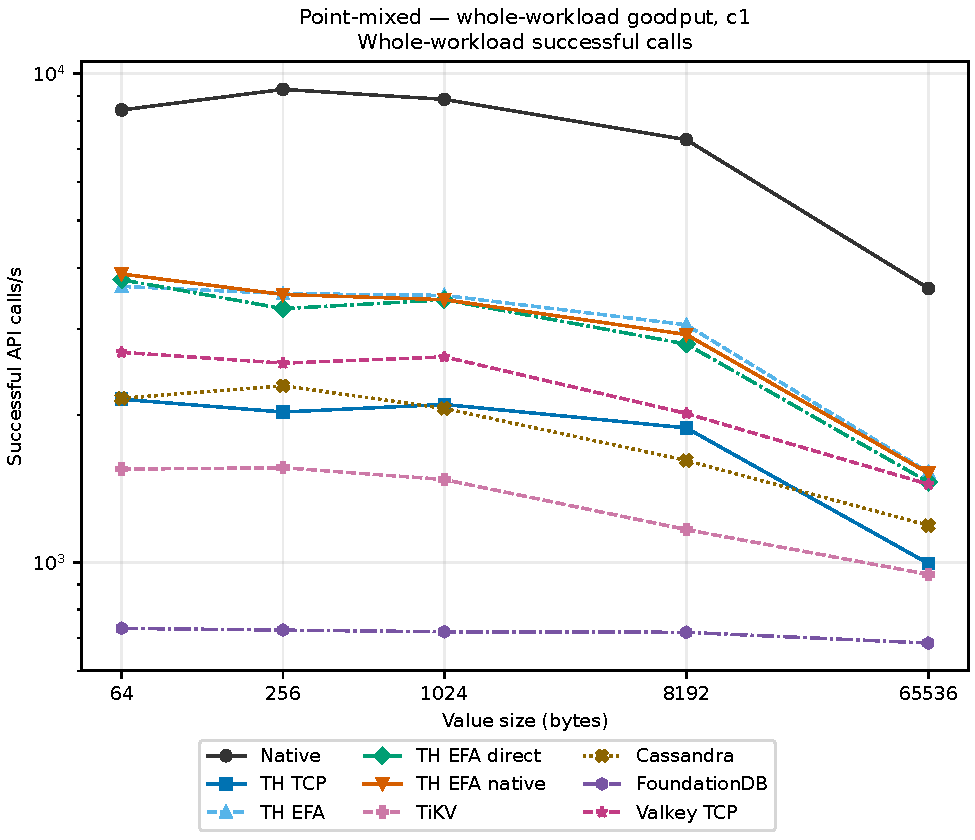
\includegraphics[page=1,width=\linewidth,height=.75\textheight,keepaspectratio]{figures/eval/panels/primary-point-mixed-goodput.pdf}\caption{Whole-workload successful calls. Primary point-mixed achieved goodput, not offered rate. One independent repetition per case; units and workload dimensions are shown in the plot.}\label{fig:eval-primary-point-mixed-goodput-1}\end{figure}
\begin{figure}[p]\centering\includegraphics[page=2,width=\linewidth,height=.75\textheight,keepaspectratio]{figures/eval/panels/primary-point-mixed-goodput.pdf}\caption{Successful logical keys. Primary point-mixed achieved goodput, not offered rate. One independent repetition per case; units and workload dimensions are shown in the plot.}\label{fig:eval-primary-point-mixed-goodput-2}\end{figure}
\begin{figure}[p]\centering\includegraphics[page=3,width=\linewidth,height=.75\textheight,keepaspectratio]{figures/eval/panels/primary-point-mixed-goodput.pdf}\caption{Successful value payload. Primary point-mixed achieved goodput, not offered rate. One independent repetition per case; units and workload dimensions are shown in the plot.}\label{fig:eval-primary-point-mixed-goodput-3}\end{figure}

\clearpage
\begin{figure}[p]\centering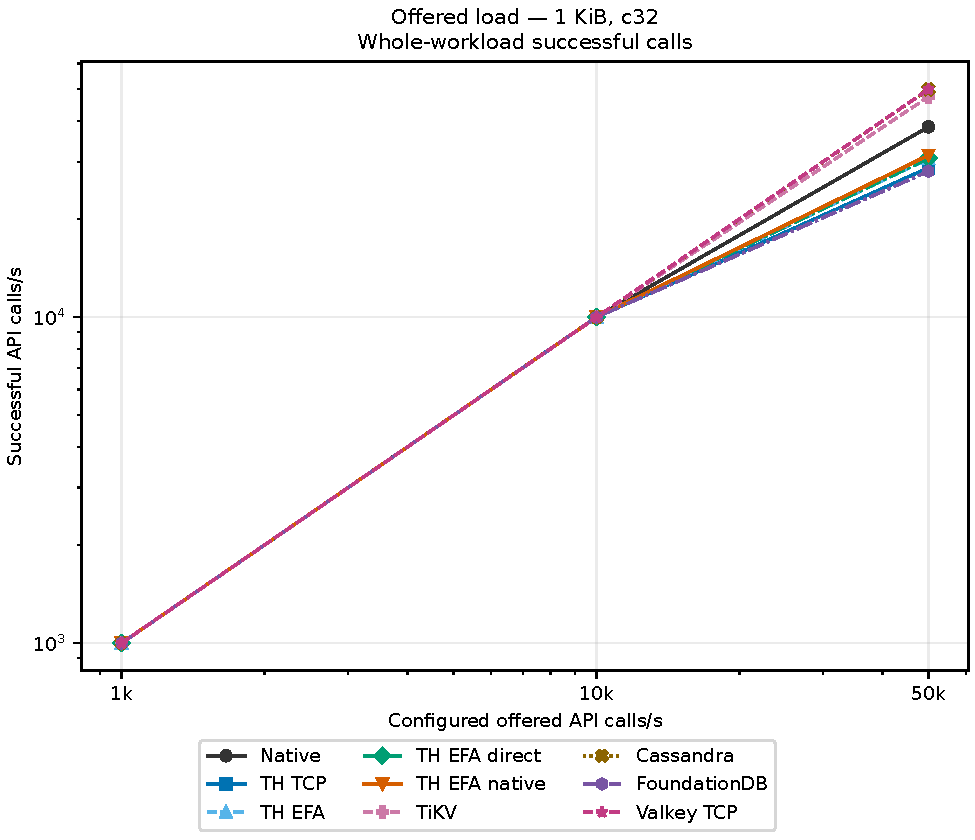
\includegraphics[page=1,width=\linewidth,height=.75\textheight,keepaspectratio]{figures/eval/panels/offered-load-accounting.pdf}\caption{Whole-workload successful calls. Offered-load successes and rejections; case completion does not imply universal admission. One independent repetition per case; units and workload dimensions are shown in the plot.}\label{fig:eval-offered-load-accounting-1}\end{figure}
\begin{figure}[p]\centering\includegraphics[page=2,width=\linewidth,height=.75\textheight,keepaspectratio]{figures/eval/panels/offered-load-accounting.pdf}\caption{Successful logical keys. Offered-load successes and rejections; case completion does not imply universal admission. One independent repetition per case; units and workload dimensions are shown in the plot.}\label{fig:eval-offered-load-accounting-2}\end{figure}
\begin{figure}[p]\centering\includegraphics[page=3,width=\linewidth,height=.75\textheight,keepaspectratio]{figures/eval/panels/offered-load-accounting.pdf}\caption{Successful value payload. Offered-load successes and rejections; case completion does not imply universal admission. One independent repetition per case; units and workload dimensions are shown in the plot.}\label{fig:eval-offered-load-accounting-3}\end{figure}
\begin{figure}[p]\centering\includegraphics[page=4,width=\linewidth,height=.75\textheight,keepaspectratio]{figures/eval/panels/offered-load-accounting.pdf}\caption{Rejected arrivals / offered arrivals. Offered-load successes and rejections; case completion does not imply universal admission. One independent repetition per case; units and workload dimensions are shown in the plot.}\label{fig:eval-offered-load-accounting-4}\end{figure}
\begin{figure}[p]\centering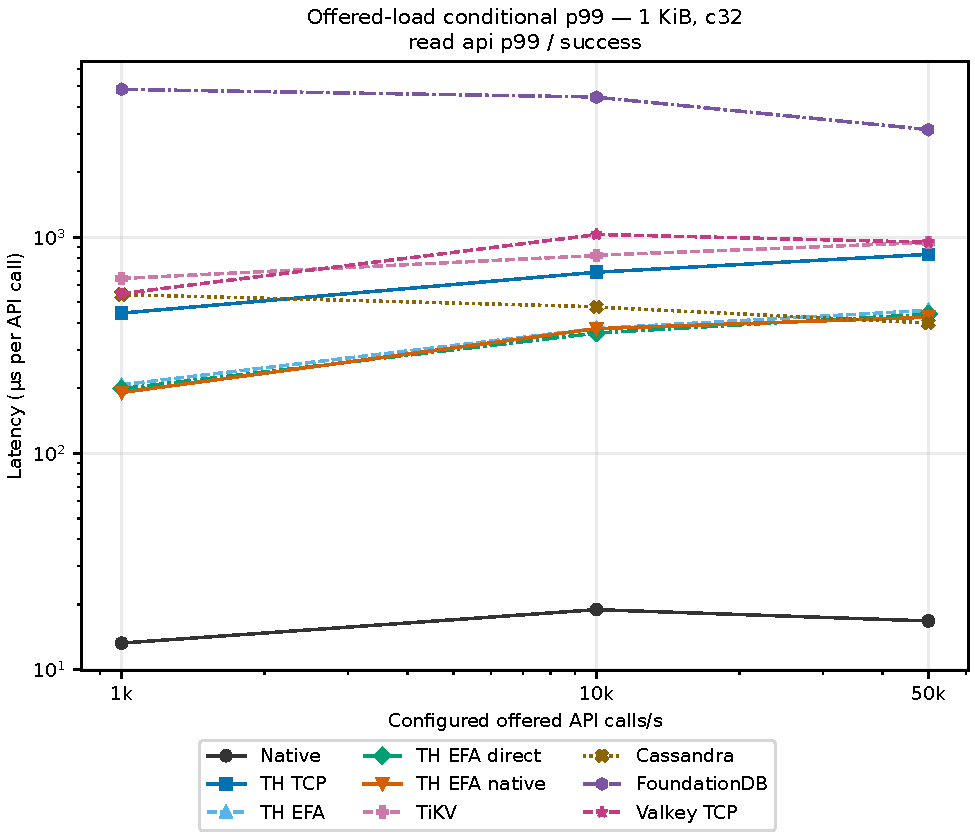
\includegraphics[page=1,width=\linewidth,height=.75\textheight,keepaspectratio]{figures/eval/panels/offered-load-tails.pdf}\caption{read api p99 / success. Offered-load latency tails by outcome; do not combine successful and rejected calls. One independent repetition per case; units and workload dimensions are shown in the plot.}\label{fig:eval-offered-load-tails-1}\end{figure}
\begin{figure}[p]\centering\includegraphics[page=2,width=\linewidth,height=.75\textheight,keepaspectratio]{figures/eval/panels/offered-load-tails.pdf}\caption{read response p99 / success. Offered-load latency tails by outcome; do not combine successful and rejected calls. One independent repetition per case; units and workload dimensions are shown in the plot.}\label{fig:eval-offered-load-tails-2}\end{figure}
\begin{figure}[p]\centering\includegraphics[page=3,width=\linewidth,height=.75\textheight,keepaspectratio]{figures/eval/panels/offered-load-tails.pdf}\caption{read scheduling p99 / success. Offered-load latency tails by outcome; do not combine successful and rejected calls. One independent repetition per case; units and workload dimensions are shown in the plot.}\label{fig:eval-offered-load-tails-3}\end{figure}
\begin{figure}[p]\centering\includegraphics[page=4,width=\linewidth,height=.75\textheight,keepaspectratio]{figures/eval/panels/offered-load-tails.pdf}\caption{put api p99 / success. Offered-load latency tails by outcome; do not combine successful and rejected calls. One independent repetition per case; units and workload dimensions are shown in the plot.}\label{fig:eval-offered-load-tails-4}\end{figure}
\begin{figure}[p]\centering\includegraphics[page=5,width=\linewidth,height=.75\textheight,keepaspectratio]{figures/eval/panels/offered-load-tails.pdf}\caption{put response p99 / success. Offered-load latency tails by outcome; do not combine successful and rejected calls. One independent repetition per case; units and workload dimensions are shown in the plot.}\label{fig:eval-offered-load-tails-5}\end{figure}
\begin{figure}[p]\centering\includegraphics[page=6,width=\linewidth,height=.75\textheight,keepaspectratio]{figures/eval/panels/offered-load-tails.pdf}\caption{put scheduling p99 / success. Offered-load latency tails by outcome; do not combine successful and rejected calls. One independent repetition per case; units and workload dimensions are shown in the plot.}\label{fig:eval-offered-load-tails-6}\end{figure}

\clearpage
\begin{figure}[p]\centering\includegraphics[page=7,width=\linewidth,height=.75\textheight,keepaspectratio]{figures/eval/panels/offered-load-tails.pdf}\caption{read response p99 / rejected. Offered-load latency tails by outcome; do not combine successful and rejected calls. One independent repetition per case; units and workload dimensions are shown in the plot.}\label{fig:eval-offered-load-tails-7}\end{figure}
\begin{figure}[p]\centering\includegraphics[page=8,width=\linewidth,height=.75\textheight,keepaspectratio]{figures/eval/panels/offered-load-tails.pdf}\caption{put response p99 / rejected. Offered-load latency tails by outcome; do not combine successful and rejected calls. One independent repetition per case; units and workload dimensions are shown in the plot.}\label{fig:eval-offered-load-tails-8}\end{figure}
\begin{figure}[p]\centering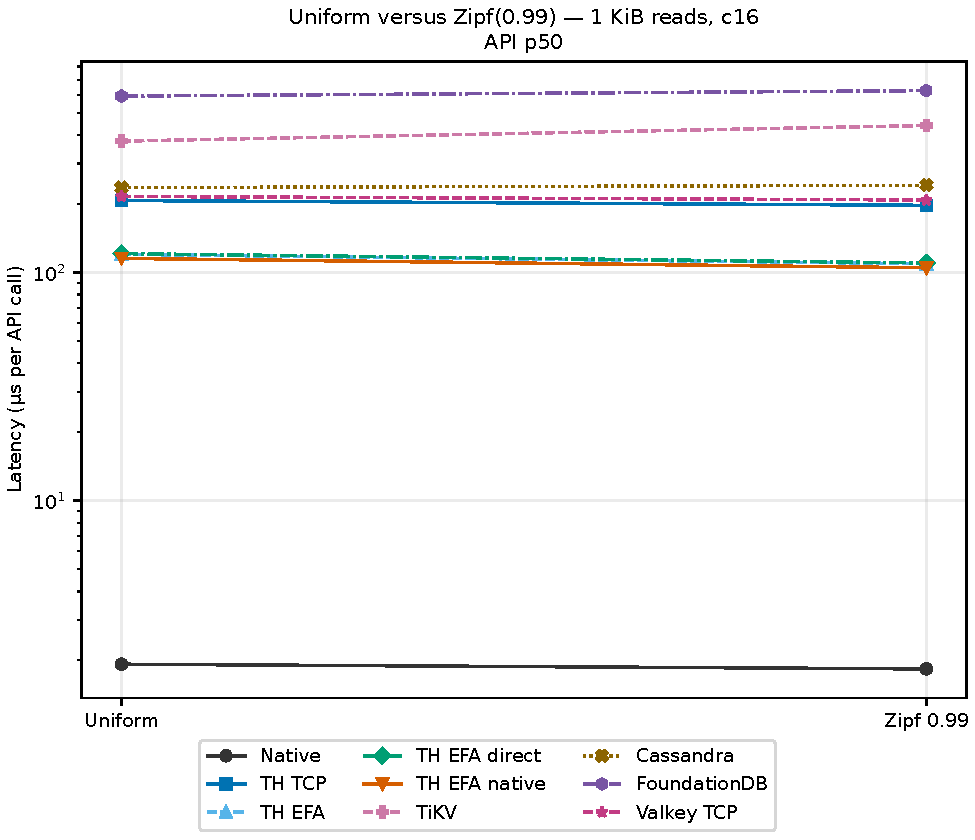
\includegraphics[page=1,width=\linewidth,height=.75\textheight,keepaspectratio]{figures/eval/panels/zipf-versus-uniform.pdf}\caption{API p50. Zipf and uniform read observations remain separate workloads. One independent repetition per case; units and workload dimensions are shown in the plot.}\label{fig:eval-zipf-versus-uniform-1}\end{figure}
\begin{figure}[p]\centering\includegraphics[page=2,width=\linewidth,height=.75\textheight,keepaspectratio]{figures/eval/panels/zipf-versus-uniform.pdf}\caption{API p99. Zipf and uniform read observations remain separate workloads. One independent repetition per case; units and workload dimensions are shown in the plot.}\label{fig:eval-zipf-versus-uniform-2}\end{figure}
\begin{figure}[p]\centering\includegraphics[page=3,width=\linewidth,height=.75\textheight,keepaspectratio]{figures/eval/panels/zipf-versus-uniform.pdf}\caption{Successful calls. Zipf and uniform read observations remain separate workloads. One independent repetition per case; units and workload dimensions are shown in the plot.}\label{fig:eval-zipf-versus-uniform-3}\end{figure}
\begin{figure}[p]\centering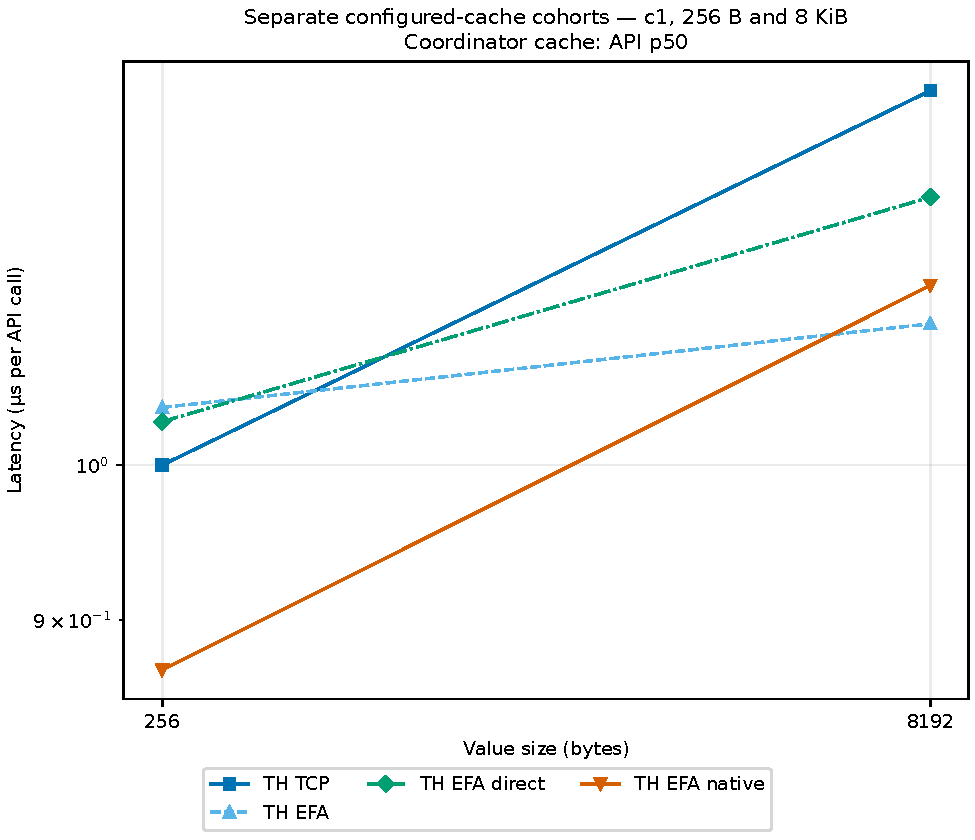
\includegraphics[page=1,width=\linewidth,height=.75\textheight,keepaspectratio]{figures/eval/panels/cache-cohorts.pdf}\caption{Coordinator cache: API p50. Configured cache cohorts; registered-RAM observations mix RMA completions and message fallbacks. One independent repetition per case; units and workload dimensions are shown in the plot.}\label{fig:eval-cache-cohorts-1}\end{figure}
\begin{figure}[p]\centering\includegraphics[page=2,width=\linewidth,height=.75\textheight,keepaspectratio]{figures/eval/panels/cache-cohorts.pdf}\caption{Coordinator cache: API p99. Configured cache cohorts; registered-RAM observations mix RMA completions and message fallbacks. One independent repetition per case; units and workload dimensions are shown in the plot.}\label{fig:eval-cache-cohorts-2}\end{figure}
\begin{figure}[p]\centering\includegraphics[page=3,width=\linewidth,height=.75\textheight,keepaspectratio]{figures/eval/panels/cache-cohorts.pdf}\caption{Coordinator cache: successful calls. Configured cache cohorts; registered-RAM observations mix RMA completions and message fallbacks. One independent repetition per case; units and workload dimensions are shown in the plot.}\label{fig:eval-cache-cohorts-3}\end{figure}
\begin{figure}[p]\centering\includegraphics[page=4,width=\linewidth,height=.75\textheight,keepaspectratio]{figures/eval/panels/cache-cohorts.pdf}\caption{Owner cache: API p50. Configured cache cohorts; registered-RAM observations mix RMA completions and message fallbacks. One independent repetition per case; units and workload dimensions are shown in the plot.}\label{fig:eval-cache-cohorts-4}\end{figure}
\begin{figure}[p]\centering\includegraphics[page=5,width=\linewidth,height=.75\textheight,keepaspectratio]{figures/eval/panels/cache-cohorts.pdf}\caption{Owner cache: API p99. Configured cache cohorts; registered-RAM observations mix RMA completions and message fallbacks. One independent repetition per case; units and workload dimensions are shown in the plot.}\label{fig:eval-cache-cohorts-5}\end{figure}

\clearpage
\begin{figure}[p]\centering\includegraphics[page=6,width=\linewidth,height=.75\textheight,keepaspectratio]{figures/eval/panels/cache-cohorts.pdf}\caption{Owner cache: successful calls. Configured cache cohorts; registered-RAM observations mix RMA completions and message fallbacks. One independent repetition per case; units and workload dimensions are shown in the plot.}\label{fig:eval-cache-cohorts-6}\end{figure}
\begin{figure}[p]\centering\includegraphics[page=7,width=\linewidth,height=.75\textheight,keepaspectratio]{figures/eval/panels/cache-cohorts.pdf}\caption{Registered RAM: API p50. Configured cache cohorts; registered-RAM observations mix RMA completions and message fallbacks. One independent repetition per case; units and workload dimensions are shown in the plot.}\label{fig:eval-cache-cohorts-7}\end{figure}
\begin{figure}[p]\centering\includegraphics[page=8,width=\linewidth,height=.75\textheight,keepaspectratio]{figures/eval/panels/cache-cohorts.pdf}\caption{Registered RAM: API p99. Configured cache cohorts; registered-RAM observations mix RMA completions and message fallbacks. One independent repetition per case; units and workload dimensions are shown in the plot.}\label{fig:eval-cache-cohorts-8}\end{figure}
\begin{figure}[p]\centering\includegraphics[page=9,width=\linewidth,height=.75\textheight,keepaspectratio]{figures/eval/panels/cache-cohorts.pdf}\caption{Registered RAM: successful calls. Configured cache cohorts; registered-RAM observations mix RMA completions and message fallbacks. One independent repetition per case; units and workload dimensions are shown in the plot.}\label{fig:eval-cache-cohorts-9}\end{figure}
\begin{figure}[p]\centering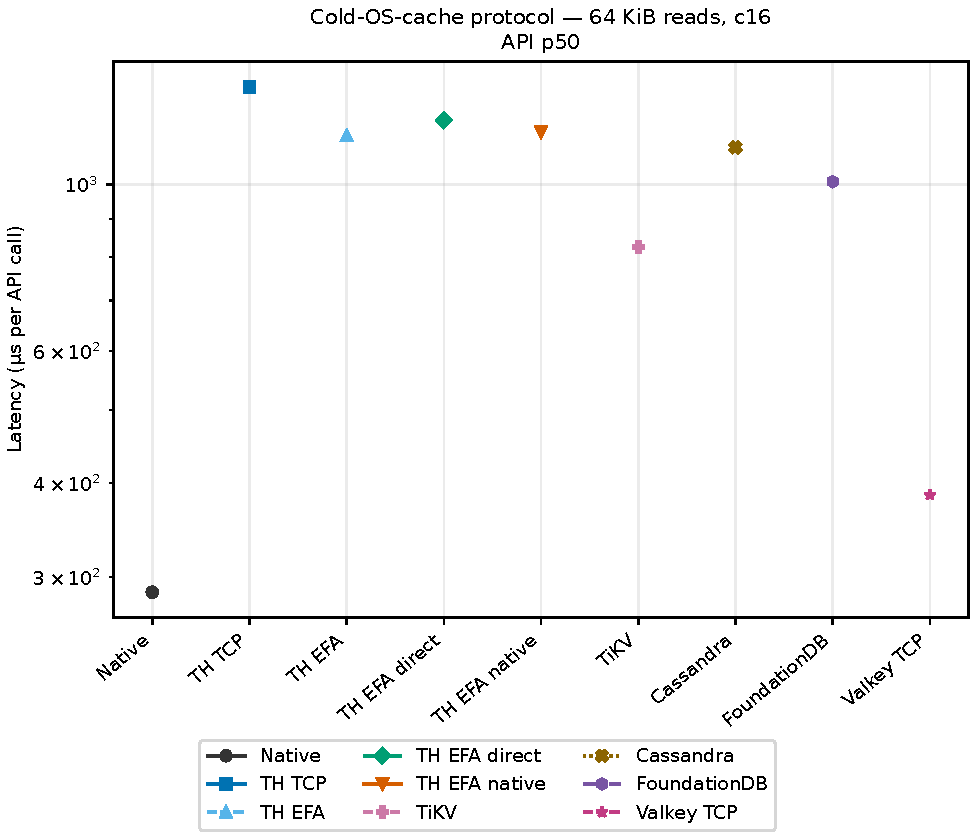
\includegraphics[page=1,width=\linewidth,height=.75\textheight,keepaspectratio]{figures/eval/panels/cold-os-cache.pdf}\caption{API p50. OS-cache-drop cohort; user-space caches and RAM datasets can remain resident. One independent repetition per case; units and workload dimensions are shown in the plot.}\label{fig:eval-cold-os-cache-1}\end{figure}
\begin{figure}[p]\centering\includegraphics[page=2,width=\linewidth,height=.75\textheight,keepaspectratio]{figures/eval/panels/cold-os-cache.pdf}\caption{API p99. OS-cache-drop cohort; user-space caches and RAM datasets can remain resident. One independent repetition per case; units and workload dimensions are shown in the plot.}\label{fig:eval-cold-os-cache-2}\end{figure}
\begin{figure}[p]\centering\includegraphics[page=3,width=\linewidth,height=.75\textheight,keepaspectratio]{figures/eval/panels/cold-os-cache.pdf}\caption{Whole-workload successful calls. OS-cache-drop cohort; user-space caches and RAM datasets can remain resident. One independent repetition per case; units and workload dimensions are shown in the plot.}\label{fig:eval-cold-os-cache-3}\end{figure}
\begin{figure}[p]\centering\includegraphics[page=4,width=\linewidth,height=.75\textheight,keepaspectratio]{figures/eval/panels/cold-os-cache.pdf}\caption{Successful logical keys. OS-cache-drop cohort; user-space caches and RAM datasets can remain resident. One independent repetition per case; units and workload dimensions are shown in the plot.}\label{fig:eval-cold-os-cache-4}\end{figure}
\begin{figure}[p]\centering\includegraphics[page=5,width=\linewidth,height=.75\textheight,keepaspectratio]{figures/eval/panels/cold-os-cache.pdf}\caption{Successful value payload. OS-cache-drop cohort; user-space caches and RAM datasets can remain resident. One independent repetition per case; units and workload dimensions are shown in the plot.}\label{fig:eval-cold-os-cache-5}\end{figure}
\begin{figure}[p]\centering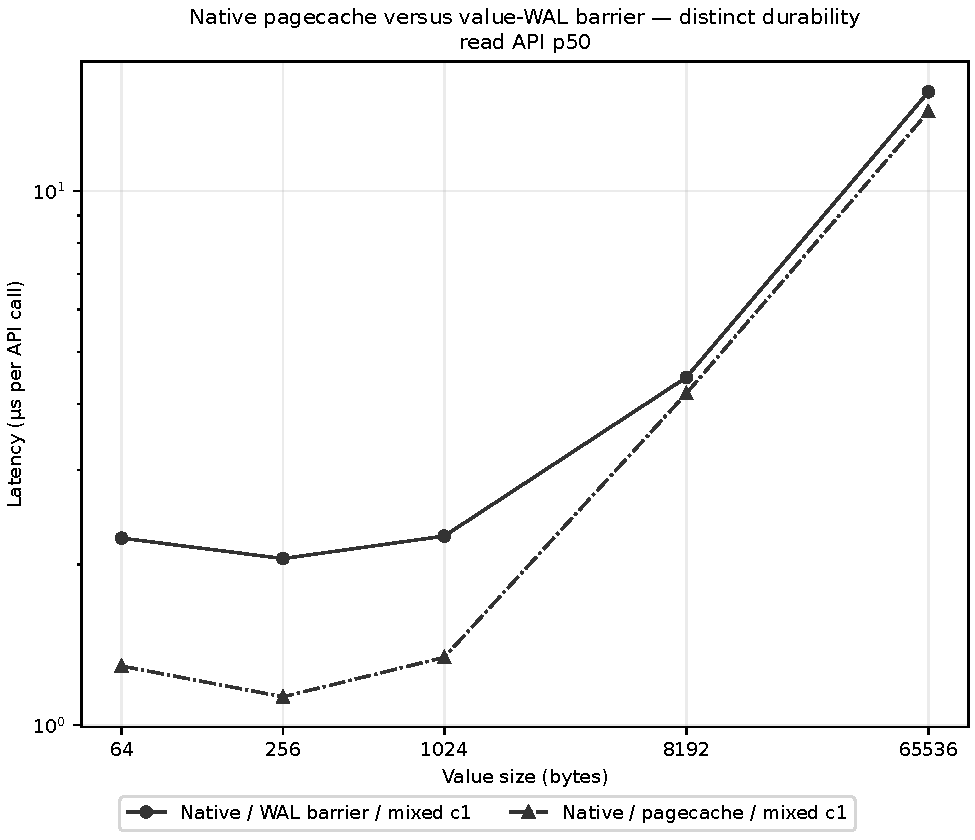
\includegraphics[page=1,width=\linewidth,height=.75\textheight,keepaspectratio]{figures/eval/panels/native-pagecache-latency.pdf}\caption{read API p50. Native page-cache acknowledgment cohort latency; not the primary Value-WAL-barrier durability tier. One independent repetition per case; units and workload dimensions are shown in the plot.}\label{fig:eval-native-pagecache-latency-1}\end{figure}

\clearpage
\begin{figure}[p]\centering\includegraphics[page=2,width=\linewidth,height=.75\textheight,keepaspectratio]{figures/eval/panels/native-pagecache-latency.pdf}\caption{put API p50. Native page-cache acknowledgment cohort latency; not the primary Value-WAL-barrier durability tier. One independent repetition per case; units and workload dimensions are shown in the plot.}\label{fig:eval-native-pagecache-latency-2}\end{figure}
\begin{figure}[p]\centering\includegraphics[page=3,width=\linewidth,height=.75\textheight,keepaspectratio]{figures/eval/panels/native-pagecache-latency.pdf}\caption{delete API p50. Native page-cache acknowledgment cohort latency; not the primary Value-WAL-barrier durability tier. One independent repetition per case; units and workload dimensions are shown in the plot.}\label{fig:eval-native-pagecache-latency-3}\end{figure}
\begin{figure}[p]\centering\includegraphics[page=4,width=\linewidth,height=.75\textheight,keepaspectratio]{figures/eval/panels/native-pagecache-latency.pdf}\caption{missing\_read API p50. Native page-cache acknowledgment cohort latency; not the primary Value-WAL-barrier durability tier. One independent repetition per case; units and workload dimensions are shown in the plot.}\label{fig:eval-native-pagecache-latency-4}\end{figure}
\begin{figure}[p]\centering\includegraphics[page=5,width=\linewidth,height=.75\textheight,keepaspectratio]{figures/eval/panels/native-pagecache-latency.pdf}\caption{get\_many API p50. Native page-cache acknowledgment cohort latency; not the primary Value-WAL-barrier durability tier. One independent repetition per case; units and workload dimensions are shown in the plot.}\label{fig:eval-native-pagecache-latency-5}\end{figure}
\begin{figure}[p]\centering\includegraphics[page=6,width=\linewidth,height=.75\textheight,keepaspectratio]{figures/eval/panels/native-pagecache-latency.pdf}\caption{read API p99. Native page-cache acknowledgment cohort latency; not the primary Value-WAL-barrier durability tier. One independent repetition per case; units and workload dimensions are shown in the plot.}\label{fig:eval-native-pagecache-latency-6}\end{figure}
\begin{figure}[p]\centering\includegraphics[page=7,width=\linewidth,height=.75\textheight,keepaspectratio]{figures/eval/panels/native-pagecache-latency.pdf}\caption{put API p99. Native page-cache acknowledgment cohort latency; not the primary Value-WAL-barrier durability tier. One independent repetition per case; units and workload dimensions are shown in the plot.}\label{fig:eval-native-pagecache-latency-7}\end{figure}
\begin{figure}[p]\centering\includegraphics[page=8,width=\linewidth,height=.75\textheight,keepaspectratio]{figures/eval/panels/native-pagecache-latency.pdf}\caption{delete API p99. Native page-cache acknowledgment cohort latency; not the primary Value-WAL-barrier durability tier. One independent repetition per case; units and workload dimensions are shown in the plot.}\label{fig:eval-native-pagecache-latency-8}\end{figure}
\begin{figure}[p]\centering\includegraphics[page=9,width=\linewidth,height=.75\textheight,keepaspectratio]{figures/eval/panels/native-pagecache-latency.pdf}\caption{missing\_read API p99. Native page-cache acknowledgment cohort latency; not the primary Value-WAL-barrier durability tier. One independent repetition per case; units and workload dimensions are shown in the plot.}\label{fig:eval-native-pagecache-latency-9}\end{figure}
\begin{figure}[p]\centering\includegraphics[page=10,width=\linewidth,height=.75\textheight,keepaspectratio]{figures/eval/panels/native-pagecache-latency.pdf}\caption{get\_many API p99. Native page-cache acknowledgment cohort latency; not the primary Value-WAL-barrier durability tier. One independent repetition per case; units and workload dimensions are shown in the plot.}\label{fig:eval-native-pagecache-latency-10}\end{figure}
\begin{figure}[p]\centering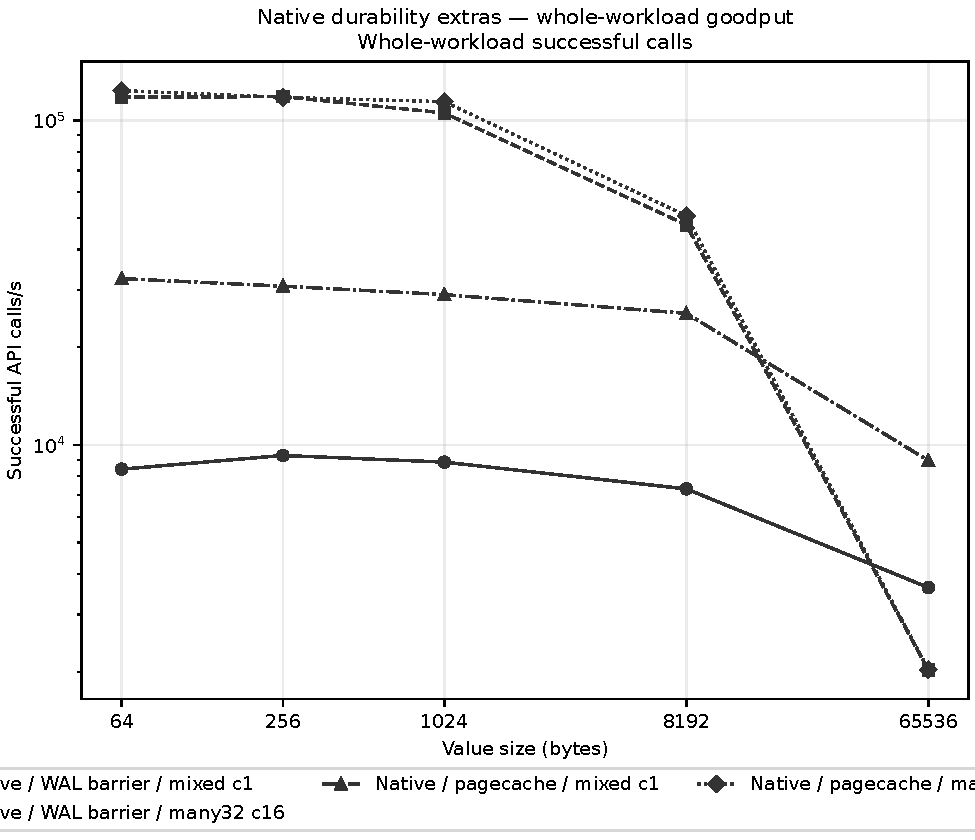
\includegraphics[page=1,width=\linewidth,height=.75\textheight,keepaspectratio]{figures/eval/panels/native-pagecache-goodput.pdf}\caption{Whole-workload successful calls. Native page-cache cohort goodput; do not equate its acknowledgment with the primary barrier. One independent repetition per case; units and workload dimensions are shown in the plot.}\label{fig:eval-native-pagecache-goodput-1}\end{figure}

\clearpage
\begin{figure}[p]\centering\includegraphics[page=2,width=\linewidth,height=.75\textheight,keepaspectratio]{figures/eval/panels/native-pagecache-goodput.pdf}\caption{Successful logical keys. Native page-cache cohort goodput; do not equate its acknowledgment with the primary barrier. One independent repetition per case; units and workload dimensions are shown in the plot.}\label{fig:eval-native-pagecache-goodput-2}\end{figure}
\begin{figure}[p]\centering\includegraphics[page=3,width=\linewidth,height=.75\textheight,keepaspectratio]{figures/eval/panels/native-pagecache-goodput.pdf}\caption{Successful value payload. Native page-cache cohort goodput; do not equate its acknowledgment with the primary barrier. One independent repetition per case; units and workload dimensions are shown in the plot.}\label{fig:eval-native-pagecache-goodput-3}\end{figure}
\begin{figure}[p]\centering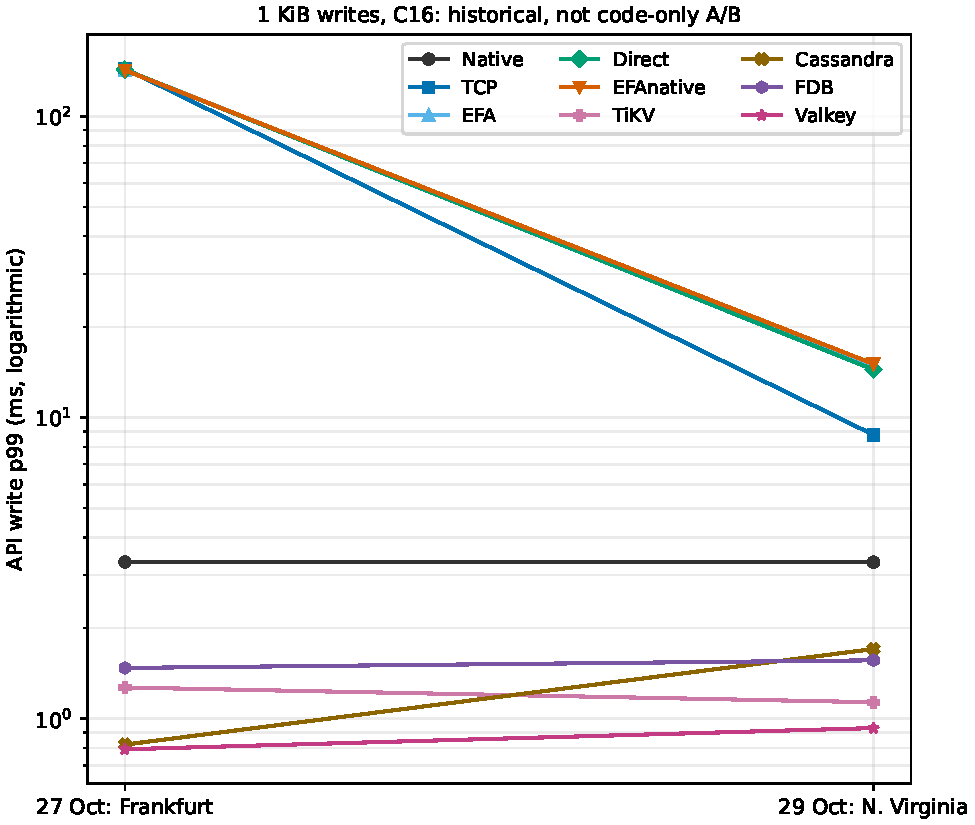
\includegraphics[width=\textwidth,height=.76\textheight,keepaspectratio]{figures/eval/historical-write-p99.pdf}\caption{Historical 1 KiB write p99: prior Frankfurt versus current North Virginia; changed region and source, not a controlled code-only comparison. One independent repetition per case; units and workload dimensions are shown in the plot.}\label{fig:eval-historical-write-p99}\end{figure}
\begin{figure}[p]\centering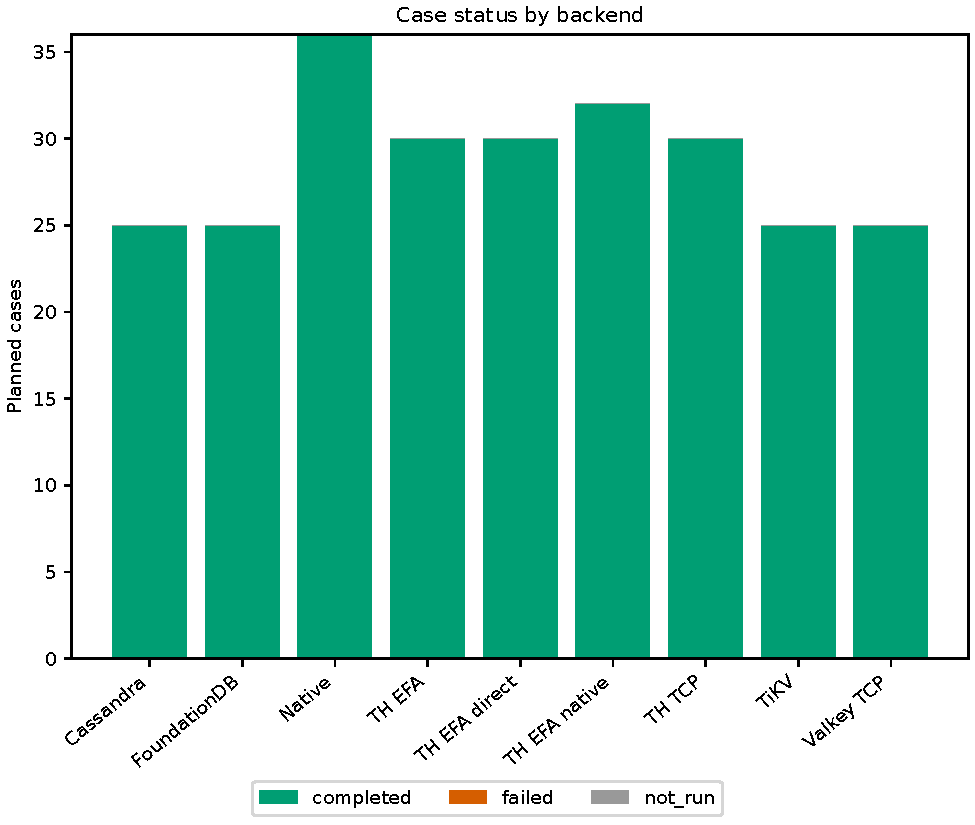
\includegraphics[page=1,width=\linewidth,height=.75\textheight,keepaspectratio]{figures/eval/panels/coverage.pdf}\caption{case status by backend.. Case coverage overview, not a complete Cartesian product of configurations. One independent repetition per case; units and workload dimensions are shown in the plot.}\label{fig:eval-coverage-1}\end{figure}
\begin{figure}[p]\centering\includegraphics[page=2,width=\linewidth,height=.75\textheight,keepaspectratio]{figures/eval/panels/coverage.pdf}\caption{case status by cohort.. Case coverage overview, not a complete Cartesian product of configurations. One independent repetition per case; units and workload dimensions are shown in the plot.}\label{fig:eval-coverage-2}\end{figure}
\clearpage

\section{Supplementary clock-statistic panels}\label{app:supplemental}
Primary RF1 successful populations only; each panel compares the indicated workload across five value sizes. The producer supplies all eight statistics; standard deviation is within-case, not a repeated-run error bar. Symmetric-log microsecond axes preserve zero. The numeric appendices retain sample counts and all outcomes. Separate clocks and populations must not be pooled.
\newgeometry{margin=0.5in}
\begin{landscape}
\begin{figure}[p]\centering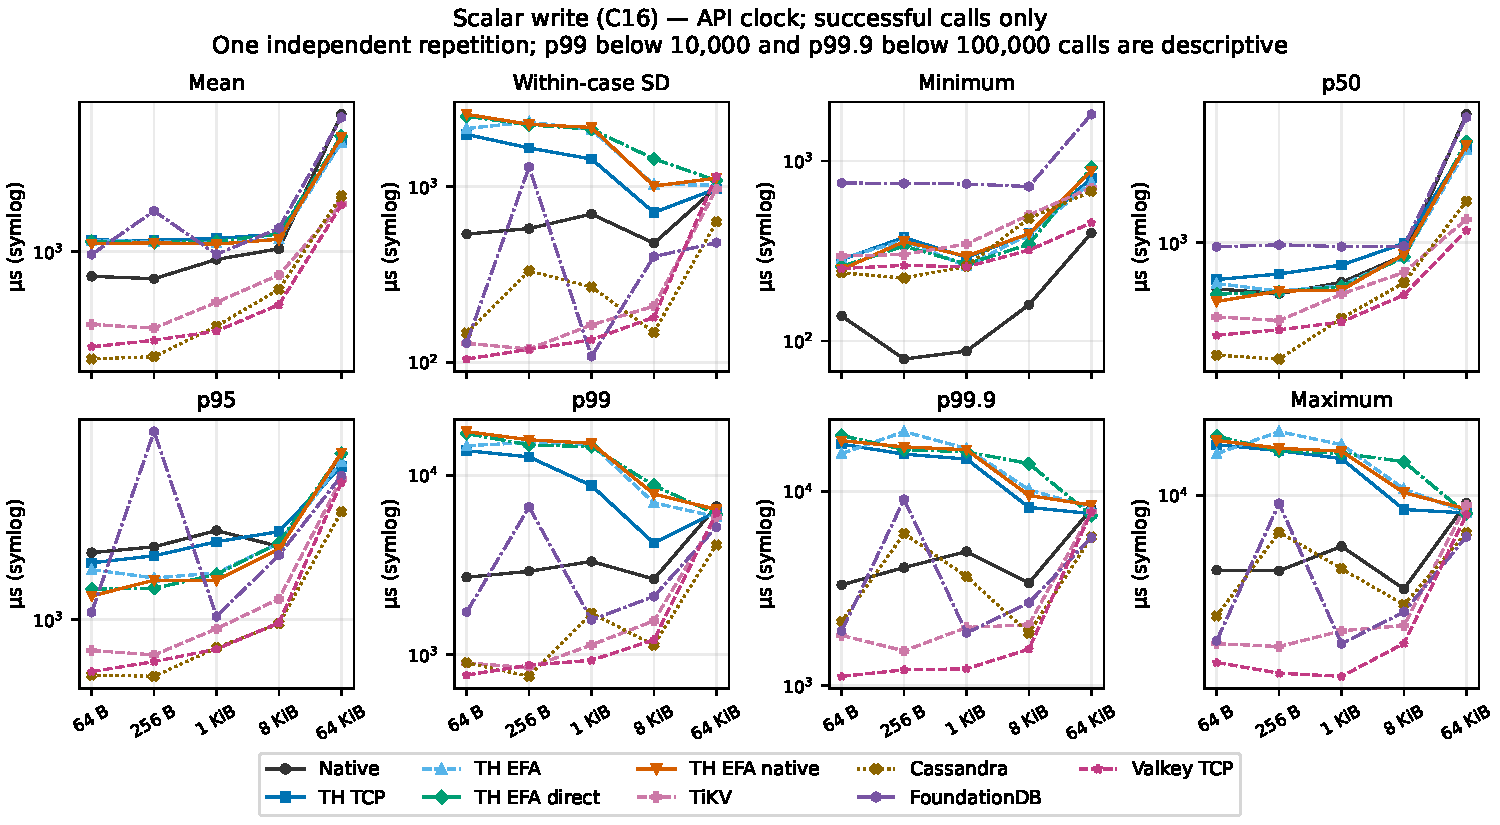
\includegraphics[page=1,width=\linewidth,height=.79\textheight,keepaspectratio]{figures/eval/supplemental-api.pdf}\caption{API clock, concurrent put; one repetition, success-only primary cohort. Mean, within-case SD, minimum, p50, p95, p99, p99.9 and maximum are separate panels. Sparse tails are descriptive; see Table~\ref{data-latencies} for counts.}\end{figure}
\begin{figure}[p]\centering\includegraphics[page=2,width=\linewidth,height=.79\textheight,keepaspectratio]{figures/eval/supplemental-api.pdf}\caption{API clock, concurrent scalar read; one repetition, success-only primary cohort. Mean, within-case SD, minimum, p50, p95, p99, p99.9 and maximum are separate panels. Sparse tails are descriptive; see Table~\ref{data-latencies} for counts.}\end{figure}
\begin{figure}[p]\centering\includegraphics[page=3,width=\linewidth,height=.79\textheight,keepaspectratio]{figures/eval/supplemental-api.pdf}\caption{API clock, concurrent 32-key get-many; one repetition, success-only primary cohort. Mean, within-case SD, minimum, p50, p95, p99, p99.9 and maximum are separate panels. Sparse tails are descriptive; see Table~\ref{data-latencies} for counts.}\end{figure}
\begin{figure}[p]\centering\includegraphics[page=4,width=\linewidth,height=.79\textheight,keepaspectratio]{figures/eval/supplemental-api.pdf}\caption{API clock, mixed read; one repetition, success-only primary cohort. Mean, within-case SD, minimum, p50, p95, p99, p99.9 and maximum are separate panels. Sparse tails are descriptive; see Table~\ref{data-latencies} for counts.}\end{figure}
\begin{figure}[p]\centering\includegraphics[page=5,width=\linewidth,height=.79\textheight,keepaspectratio]{figures/eval/supplemental-api.pdf}\caption{API clock, mixed put; one repetition, success-only primary cohort. Mean, within-case SD, minimum, p50, p95, p99, p99.9 and maximum are separate panels. Sparse tails are descriptive; see Table~\ref{data-latencies} for counts.}\end{figure}

\clearpage
\begin{figure}[p]\centering\includegraphics[page=6,width=\linewidth,height=.79\textheight,keepaspectratio]{figures/eval/supplemental-api.pdf}\caption{API clock, mixed delete; one repetition, success-only primary cohort. Mean, within-case SD, minimum, p50, p95, p99, p99.9 and maximum are separate panels. Sparse tails are descriptive; see Table~\ref{data-latencies} for counts.}\end{figure}
\begin{figure}[p]\centering\includegraphics[page=7,width=\linewidth,height=.79\textheight,keepaspectratio]{figures/eval/supplemental-api.pdf}\caption{API clock, mixed missing-read; one repetition, success-only primary cohort. Mean, within-case SD, minimum, p50, p95, p99, p99.9 and maximum are separate panels. Sparse tails are descriptive; see Table~\ref{data-latencies} for counts.}\end{figure}
\begin{figure}[p]\centering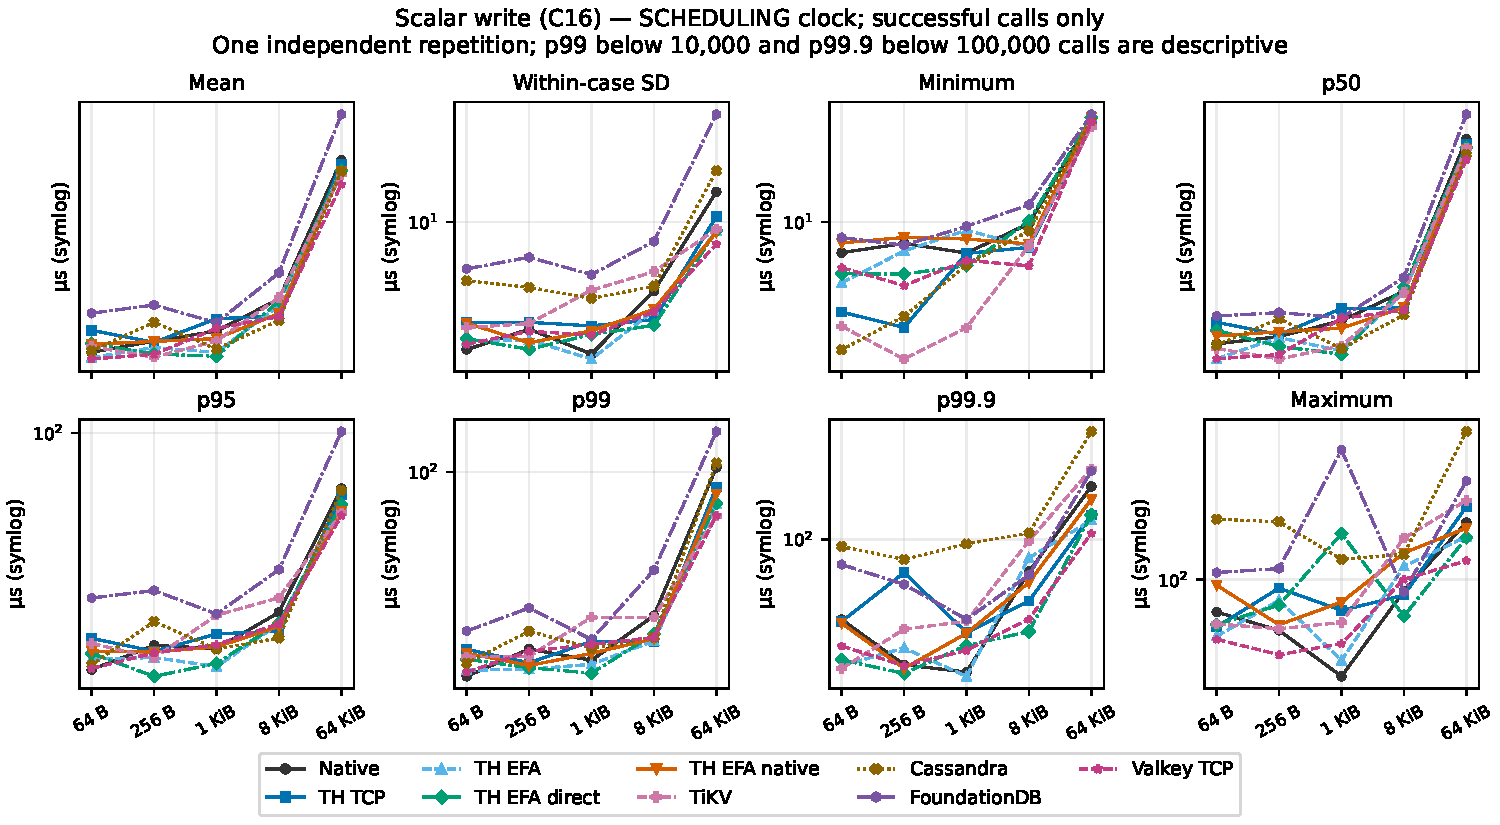
\includegraphics[page=1,width=\linewidth,height=.79\textheight,keepaspectratio]{figures/eval/supplemental-scheduling.pdf}\caption{SCHEDULING clock, concurrent put; one repetition, success-only primary cohort. Mean, within-case SD, minimum, p50, p95, p99, p99.9 and maximum are separate panels. Sparse tails are descriptive; see Table~\ref{data-latencies} for counts.}\end{figure}
\begin{figure}[p]\centering\includegraphics[page=2,width=\linewidth,height=.79\textheight,keepaspectratio]{figures/eval/supplemental-scheduling.pdf}\caption{SCHEDULING clock, concurrent scalar read; one repetition, success-only primary cohort. Mean, within-case SD, minimum, p50, p95, p99, p99.9 and maximum are separate panels. Sparse tails are descriptive; see Table~\ref{data-latencies} for counts.}\end{figure}
\begin{figure}[p]\centering\includegraphics[page=3,width=\linewidth,height=.79\textheight,keepaspectratio]{figures/eval/supplemental-scheduling.pdf}\caption{SCHEDULING clock, concurrent 32-key get-many; one repetition, success-only primary cohort. Mean, within-case SD, minimum, p50, p95, p99, p99.9 and maximum are separate panels. Sparse tails are descriptive; see Table~\ref{data-latencies} for counts.}\end{figure}
\begin{figure}[p]\centering\includegraphics[page=4,width=\linewidth,height=.79\textheight,keepaspectratio]{figures/eval/supplemental-scheduling.pdf}\caption{SCHEDULING clock, mixed read; one repetition, success-only primary cohort. Mean, within-case SD, minimum, p50, p95, p99, p99.9 and maximum are separate panels. Sparse tails are descriptive; see Table~\ref{data-latencies} for counts.}\end{figure}
\begin{figure}[p]\centering\includegraphics[page=5,width=\linewidth,height=.79\textheight,keepaspectratio]{figures/eval/supplemental-scheduling.pdf}\caption{SCHEDULING clock, mixed put; one repetition, success-only primary cohort. Mean, within-case SD, minimum, p50, p95, p99, p99.9 and maximum are separate panels. Sparse tails are descriptive; see Table~\ref{data-latencies} for counts.}\end{figure}
\begin{figure}[p]\centering\includegraphics[page=6,width=\linewidth,height=.79\textheight,keepaspectratio]{figures/eval/supplemental-scheduling.pdf}\caption{SCHEDULING clock, mixed delete; one repetition, success-only primary cohort. Mean, within-case SD, minimum, p50, p95, p99, p99.9 and maximum are separate panels. Sparse tails are descriptive; see Table~\ref{data-latencies} for counts.}\end{figure}
\begin{figure}[p]\centering\includegraphics[page=7,width=\linewidth,height=.79\textheight,keepaspectratio]{figures/eval/supplemental-scheduling.pdf}\caption{SCHEDULING clock, mixed missing-read; one repetition, success-only primary cohort. Mean, within-case SD, minimum, p50, p95, p99, p99.9 and maximum are separate panels. Sparse tails are descriptive; see Table~\ref{data-latencies} for counts.}\end{figure}
\begin{figure}[p]\centering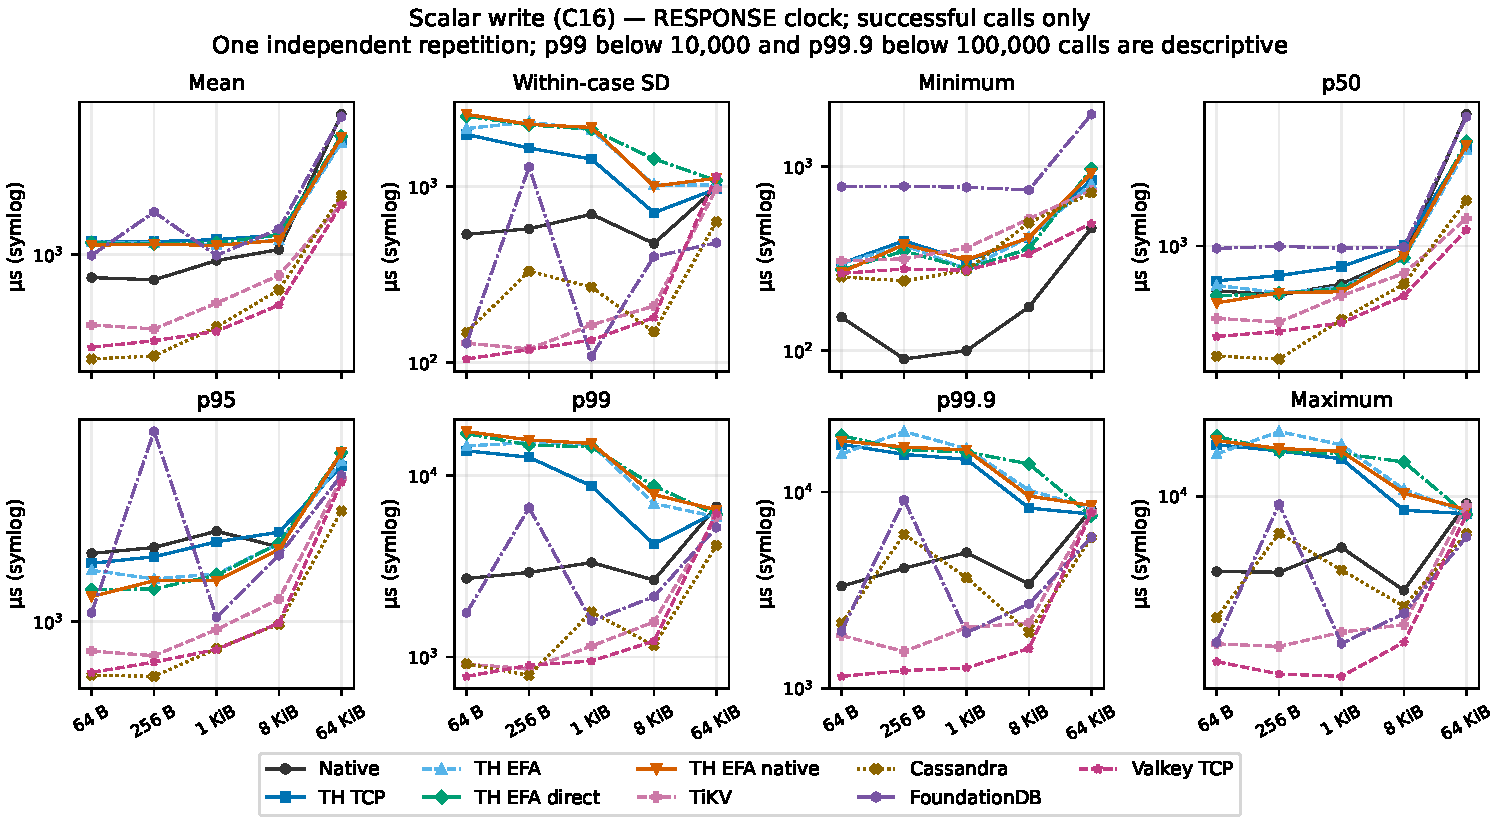
\includegraphics[page=1,width=\linewidth,height=.79\textheight,keepaspectratio]{figures/eval/supplemental-response.pdf}\caption{RESPONSE clock, concurrent put; one repetition, success-only primary cohort. Mean, within-case SD, minimum, p50, p95, p99, p99.9 and maximum are separate panels. Sparse tails are descriptive; see Table~\ref{data-latencies} for counts.}\end{figure}

\clearpage
\begin{figure}[p]\centering\includegraphics[page=2,width=\linewidth,height=.79\textheight,keepaspectratio]{figures/eval/supplemental-response.pdf}\caption{RESPONSE clock, concurrent scalar read; one repetition, success-only primary cohort. Mean, within-case SD, minimum, p50, p95, p99, p99.9 and maximum are separate panels. Sparse tails are descriptive; see Table~\ref{data-latencies} for counts.}\end{figure}
\begin{figure}[p]\centering\includegraphics[page=3,width=\linewidth,height=.79\textheight,keepaspectratio]{figures/eval/supplemental-response.pdf}\caption{RESPONSE clock, concurrent 32-key get-many; one repetition, success-only primary cohort. Mean, within-case SD, minimum, p50, p95, p99, p99.9 and maximum are separate panels. Sparse tails are descriptive; see Table~\ref{data-latencies} for counts.}\end{figure}
\begin{figure}[p]\centering\includegraphics[page=4,width=\linewidth,height=.79\textheight,keepaspectratio]{figures/eval/supplemental-response.pdf}\caption{RESPONSE clock, mixed read; one repetition, success-only primary cohort. Mean, within-case SD, minimum, p50, p95, p99, p99.9 and maximum are separate panels. Sparse tails are descriptive; see Table~\ref{data-latencies} for counts.}\end{figure}
\begin{figure}[p]\centering\includegraphics[page=5,width=\linewidth,height=.79\textheight,keepaspectratio]{figures/eval/supplemental-response.pdf}\caption{RESPONSE clock, mixed put; one repetition, success-only primary cohort. Mean, within-case SD, minimum, p50, p95, p99, p99.9 and maximum are separate panels. Sparse tails are descriptive; see Table~\ref{data-latencies} for counts.}\end{figure}
\begin{figure}[p]\centering\includegraphics[page=6,width=\linewidth,height=.79\textheight,keepaspectratio]{figures/eval/supplemental-response.pdf}\caption{RESPONSE clock, mixed delete; one repetition, success-only primary cohort. Mean, within-case SD, minimum, p50, p95, p99, p99.9 and maximum are separate panels. Sparse tails are descriptive; see Table~\ref{data-latencies} for counts.}\end{figure}
\begin{figure}[p]\centering\includegraphics[page=7,width=\linewidth,height=.79\textheight,keepaspectratio]{figures/eval/supplemental-response.pdf}\caption{RESPONSE clock, mixed missing-read; one repetition, success-only primary cohort. Mean, within-case SD, minimum, p50, p95, p99, p99.9 and maximum are separate panels. Sparse tails are descriptive; see Table~\ref{data-latencies} for counts.}\end{figure}
\clearpage
\end{landscape}
\restoregeometry

\section{Experimental matrix and backend contracts}\label{app:matrix}
\begin{landscape}
\scriptsize
\setlength{\tabcolsep}{2pt}
\sloppy
\begin{longtable}{p{3cm}p{2.5cm}p{3.1cm}rrrp{7cm}}
\caption{Exact case matrix: 258 cases, one repetition each; key counts are in the case index. TCP/EFA/Direct/EFAnative denote Tidehunter variants; FDB denotes FoundationDB; Valkey denotes Valkey TCP. Backend names and values refer to observed cases, not a claim of every possible combination.}\label{data-matrix}\\
\toprule
Cohort & Profile & Value bytes & C & Offered/s & Cases & Backends\\
\midrule
\endfirsthead
\toprule
Cohort & Profile & Value bytes & C & Offered/s & Cases & Backends\\
\midrule
\endhead
\bottomrule
\endfoot
cold\_\allowbreak{}os\_\allowbreak{}cache & cold-os-large & 65536 & 16 & -- & 9 & Cassandra, FDB, Native, EFA, Direct, EFAnative, TCP, TiKV, Valkey\\
coordinator\_\allowbreak{}cache\_\allowbreak{}configured & coordinator-cache & 256, 8192 & 1 & -- & 8 & EFA, Direct, EFAnative, TCP\\
native\_\allowbreak{}pagecache & point-mixed & 64, 256, 1024, 8192, 65536 & 1 & -- & 5 & Native\\
native\_\allowbreak{}pagecache & read-many32 & 64, 256, 1024, 8192, 65536 & 16 & -- & 5 & Native\\
owner\_\allowbreak{}cache\_\allowbreak{}configured & owner-cache & 256, 8192 & 1 & -- & 8 & EFA, Direct, EFAnative, TCP\\
primary\_\allowbreak{}rf1 & offered-1000 & 1024 & 32 & 1000 & 9 & Cassandra, FDB, Native, EFA, Direct, EFAnative, TCP, TiKV, Valkey\\
primary\_\allowbreak{}rf1 & offered-10000 & 1024 & 32 & 10000 & 9 & Cassandra, FDB, Native, EFA, Direct, EFAnative, TCP, TiKV, Valkey\\
primary\_\allowbreak{}rf1 & offered-50000 & 1024 & 32 & 50000 & 9 & Cassandra, FDB, Native, EFA, Direct, EFAnative, TCP, TiKV, Valkey\\
primary\_\allowbreak{}rf1 & point-mixed & 64, 256, 1024, 8192, 65536 & 1 & -- & 45 & Cassandra, FDB, Native, EFA, Direct, EFAnative, TCP, TiKV, Valkey\\
primary\_\allowbreak{}rf1 & read-concurrent & 64, 256, 1024, 8192, 65536 & 16 & -- & 45 & Cassandra, FDB, Native, EFA, Direct, EFAnative, TCP, TiKV, Valkey\\
primary\_\allowbreak{}rf1 & read-many32 & 64, 256, 1024, 8192, 65536 & 16 & -- & 45 & Cassandra, FDB, Native, EFA, Direct, EFAnative, TCP, TiKV, Valkey\\
primary\_\allowbreak{}rf1 & write-concurrent & 64, 256, 1024, 8192, 65536 & 16 & -- & 45 & Cassandra, FDB, Native, EFA, Direct, EFAnative, TCP, TiKV, Valkey\\
primary\_\allowbreak{}rf1 & zipf-read & 1024 & 16 & -- & 9 & Cassandra, FDB, Native, EFA, Direct, EFAnative, TCP, TiKV, Valkey\\
registered\_\allowbreak{}ram\_\allowbreak{}configured & registered-ram & 256, 8192 & 1 & -- & 2 & EFAnative\\
write\_\allowbreak{}stage\_\allowbreak{}diagnostics & write-concurrent & 1024 & 16 & -- & 5 & Native, EFA, Direct, EFAnative, TCP\\
\end{longtable}
\normalsize
\end{landscape}



\begin{landscape}
\scriptsize
\setlength{\tabcolsep}{2pt}
\sloppy
\begin{longtable}{p{2cm}p{5cm}p{4.4cm}p{5cm}p{2cm}}
\caption{Observed primary RF1 backend contracts from comparison.json; device persistence and security settings are not inferred. TCP/EFA/Direct/EFAnative denote Tidehunter variants; FDB denotes FoundationDB; Valkey denotes Valkey TCP. Atomicity describes adapter metadata, not a measured batch-write benchmark. Full configuration and version evidence are in data/backend-contracts.json and data/comparison.json.}\label{data-backend-contracts}\\
\toprule
Backend & Acknowledgement & Consistency & get-many implementation & Batch atomicity\\
\midrule
\endfirsthead
\toprule
Backend & Acknowledgement & Consistency & get-many implementation & Batch atomicity\\
\midrule
\endhead
\bottomrule
\endfoot
Cassandra & CQL write acknowledged at Quorum; durable\_\allowbreak{}writes=true observed; commitlog fsync policy and physical device persistence not verified & Quorum configured on each prepared read/write/delete and logged batch & bounded per-key prepared-query fanout (limit 16); no native CQL batch GET & crash\_\allowbreak{}recovery\\
FDB & successful FDB transaction commit using the observed cluster storage-replication configuration; physical device fsync policy not independently verified & FoundationDB serializable transaction semantics & one serializable transaction, sequential native transaction gets, exact caller order & serializable\_\allowbreak{}transaction\\
Native & native write acknowledgement followed by explicit Value-WAL file persistence barrier & native Tidehunter Db keyspace semantics & ordered scalar Db::get calls; returned Bytes retained without copying & crash\_\allowbreak{}recovery\\
EFA & RF1 complete Value-WAL batch persisted on the configured owner; no replication & single coordinator NativeIndex with complete-batch owner allocation; RF1; no replication, serializable multi-key transaction, or failover & distributed ordered grouped reads; one result per caller key & crash\_\allowbreak{}recovery\\
Direct & RF1 complete Value-WAL batch persisted on the configured owner; no replication & single coordinator NativeIndex with complete-batch owner allocation; RF1; no replication, serializable multi-key transaction, or failover & distributed ordered grouped reads; one result per caller key & crash\_\allowbreak{}recovery\\
EFAnative & RF1 complete Value-WAL batch persisted on the configured owner; no replication & single coordinator NativeIndex with complete-batch owner allocation; RF1; no replication, serializable multi-key transaction, or failover & distributed ordered grouped reads; one result per caller key & crash\_\allowbreak{}recovery\\
TCP & RF1 complete Value-WAL batch persisted on the configured owner; no replication & single coordinator NativeIndex with complete-batch owner allocation; RF1; no replication, serializable multi-key transaction, or failover & distributed ordered grouped reads; one result per caller key & crash\_\allowbreak{}recovery\\
TiKV & RawKV request success; TiKV/PD acknowledgement policy is server-defined; device fsync is not independently verified & TiKV RawKV single-key semantics; no transaction isolation; batch commands are non-atomic & TiKV native RawKV batch\_\allowbreak{}get; missing keys are restored as None and results reordered to caller order & unsupported\\
Valkey & SET success reply; primary appendonly=yes, appendfsync=always, no-appendfsync-on-rewrite=no observed at admission; Valkey AOF fsyncs before replying; no replica acknowledgement & primary-routed reads/writes; RF1, no replica reads & one MGET through redis-rs; client splits by slot and reassembles input order, duplicates and nil misses & unsupported\\
\end{longtable}
\normalsize
\end{landscape}



\section{Case index and throughput}\label{app:cases}
\begin{landscape}
\scriptsize
\setlength{\tabcolsep}{2pt}
\sloppy
\begin{longtable}{llllrrrrrrrrrrr}
\caption{Case index and whole-case throughput. Backend abbreviations: TCP/EFA/Direct/EFAnative denote Tidehunter variants; FDB denotes FoundationDB; Valkey denotes Valkey TCP. Cohorts P, Cold, Coord, Owner, RMA, Page and Diag denote primary RF1, cold OS cache, coordinator cache, owner cache, registered RAM, native page cache and write diagnostics respectively. Profiles Write, Read, Batch32, Mixed, Zipf and Load denote concurrent write, concurrent read, 32-key read, point mixed, Zipf read and offered-load cases; Cold, Coord, Owner and RMA denote the matching cohort profiles. C denotes concurrency; offered rate is blank for closed-loop cases. MiB/s is successful value bandwidth. Full case IDs and unrounded precision are in data/all-results.csv.}\label{data-cases}\\
\toprule
ID & Backend & Cohort & Profile & B & Keys & C & Offered/s & Calls & OK & Rej. & s & OK/s & Keys/s & MiB/s\\
\midrule
\endfirsthead
\toprule
ID & Backend & Cohort & Profile & B & Keys & C & Offered/s & Calls & OK & Rej. & s & OK/s & Keys/s & MiB/s\\
\midrule
\endhead
\bottomrule
\endfoot
C0000 & FDB & P & Batch32 & 8192 & 4096 & 16 & -- & 2048 & 2048 & 0 & 1.8483 & 1108 & 35457 & 277.01\\
C0001 & FDB & P & Batch32 & 65536 & 4096 & 16 & -- & 2048 & 2048 & 0 & 5.2578 & 389.52 & 12465 & 779.04\\
C0002 & FDB & P & Batch32 & 256 & 4096 & 16 & -- & 2048 & 2048 & 0 & 1.1814 & 1733.6 & 55475 & 13.544\\
C0003 & FDB & P & Read & 65536 & 4096 & 16 & -- & 8192 & 8192 & 0 & 0.53646 & 15270 & 15270 & 954.4\\
C0004 & FDB & P & Mixed & 64 & 4096 & 1 & -- & 8192 & 8192 & 0 & 11.187 & 732.25 & 732.25 & 0.039641\\
C0005 & FDB & P & Write & 65536 & 4096 & 16 & -- & 4096 & 4096 & 0 & 0.8313 & 4927.2 & 4927.2 & 307.95\\
C0006 & FDB & P & Load1k & 1024 & 4096 & 32 & 1000 & 8000 & 8000 & 0 & 8.0006 & 999.92 & 999.92 & 0.97649\\
C0007 & FDB & P & Write & 64 & 4096 & 16 & -- & 4096 & 4096 & 0 & 0.26689 & 15347 & 15347 & 0.93672\\
C0008 & FDB & P & Read & 256 & 4096 & 16 & -- & 8192 & 8192 & 0 & 0.34178 & 23969 & 23969 & 5.8517\\
C0009 & FDB & P & Write & 256 & 4096 & 16 & -- & 4096 & 4096 & 0 & 0.37858 & 10819 & 10819 & 2.6414\\
C0010 & FDB & P & Read & 8192 & 4096 & 16 & -- & 8192 & 8192 & 0 & 0.39243 & 20875 & 20875 & 163.09\\
C0011 & FDB & P & Write & 1024 & 4096 & 16 & -- & 4096 & 4096 & 0 & 0.26541 & 15432 & 15432 & 15.071\\
C0012 & FDB & P & Load10k & 1024 & 4096 & 32 & 10000 & 80000 & 80000 & 0 & 8.0057 & 9992.9 & 9992.9 & 9.7587\\
C0013 & FDB & P & Read & 1024 & 4096 & 16 & -- & 8192 & 8192 & 0 & 0.32539 & 25176 & 25176 & 24.586\\
C0014 & FDB & P & Mixed & 65536 & 4096 & 1 & -- & 8192 & 8192 & 0 & 11.991 & 683.19 & 683.19 & 37.873\\
C0015 & FDB & P & Mixed & 1024 & 4096 & 1 & -- & 8192 & 8192 & 0 & 11.368 & 720.64 & 720.64 & 0.6242\\
C0016 & FDB & P & Load50k & 1024 & 4096 & 32 & 50000 & 400000 & 224451 & 175549 & 8.0123 & 28013 & 28013 & 27.357\\
C0017 & FDB & P & Mixed & 256 & 4096 & 1 & -- & 8192 & 8192 & 0 & 11.28 & 726.21 & 726.21 & 0.15726\\
C0018 & FDB & P & Batch32 & 1024 & 4096 & 16 & -- & 2048 & 2048 & 0 & 1.2749 & 1606.4 & 51406 & 50.201\\
C0019 & FDB & P & Write & 8192 & 4096 & 16 & -- & 4096 & 4096 & 0 & 0.33113 & 12370 & 12370 & 96.638\\
C0020 & FDB & P & Zipf & 1024 & 4096 & 16 & -- & 8192 & 8192 & 0 & 0.34295 & 23887 & 23887 & 23.327\\
C0021 & FDB & P & Read & 64 & 4096 & 16 & -- & 8192 & 8192 & 0 & 0.30842 & 26561 & 26561 & 1.6211\\
C0022 & FDB & P & Batch32 & 64 & 4096 & 16 & -- & 2048 & 2048 & 0 & 1.2151 & 1685.4 & 53933 & 3.2918\\
C0023 & FDB & P & Mixed & 8192 & 4096 & 1 & -- & 8192 & 8192 & 0 & 11.401 & 718.56 & 718.56 & 4.9792\\
C0024 & FDB & Cold & Cold & 65536 & 131072 & 16 & -- & 4096 & 4096 & 0 & 0.29268 & 13995 & 13995 & 874.68\\
C0025 & Valkey & P & Batch32 & 8192 & 4096 & 16 & -- & 2048 & 2048 & 0 & 0.52773 & 3880.8 & 1.2418e+05 & 970.19\\
C0026 & Valkey & P & Batch32 & 65536 & 4096 & 16 & -- & 2048 & 2048 & 0 & 1.4127 & 1449.7 & 46390 & 2899.4\\
C0027 & Valkey & P & Batch32 & 256 & 4096 & 16 & -- & 2048 & 2048 & 0 & 0.34413 & 5951.2 & 1.9044e+05 & 46.494\\
C0028 & Valkey & P & Read & 65536 & 4096 & 16 & -- & 8192 & 8192 & 0 & 0.22994 & 35627 & 35627 & 2226.7\\
C0029 & Valkey & P & Mixed & 64 & 4096 & 1 & -- & 8192 & 8192 & 0 & 3.048 & 2687.7 & 2687.7 & 0.1455\\
C0030 & Valkey & P & Write & 65536 & 4096 & 16 & -- & 4096 & 4096 & 0 & 0.39778 & 10297 & 10297 & 643.57\\
C0031 & Valkey & P & Load1k & 1024 & 4096 & 32 & 1000 & 8000 & 8000 & 0 & 8 & 999.99 & 999.99 & 0.97656\\
C0032 & Valkey & P & Write & 64 & 4096 & 16 & -- & 4096 & 4096 & 0 & 0.12354 & 33154 & 33154 & 2.0236\\
C0033 & Valkey & P & Read & 256 & 4096 & 16 & -- & 8192 & 8192 & 0 & 0.12626 & 64883 & 64883 & 15.841\\
C0034 & Valkey & P & Write & 256 & 4096 & 16 & -- & 4096 & 4096 & 0 & 0.12883 & 31795 & 31795 & 7.7624\\
C0035 & Valkey & P & Read & 8192 & 4096 & 16 & -- & 8192 & 8192 & 0 & 0.14359 & 57050 & 57050 & 445.71\\
C0036 & Valkey & P & Write & 1024 & 4096 & 16 & -- & 4096 & 4096 & 0 & 0.13965 & 29331 & 29331 & 28.643\\
C0037 & Valkey & P & Load10k & 1024 & 4096 & 32 & 10000 & 80000 & 80000 & 0 & 8.0018 & 9997.8 & 9997.8 & 9.7634\\
C0038 & Valkey & P & Read & 1024 & 4096 & 16 & -- & 8192 & 8192 & 0 & 0.13149 & 62301 & 62301 & 60.841\\
C0039 & Valkey & P & Mixed & 65536 & 4096 & 1 & -- & 8192 & 8192 & 0 & 5.6735 & 1443.9 & 1443.9 & 80.043\\
C0040 & Valkey & P & Mixed & 1024 & 4096 & 1 & -- & 8192 & 8192 & 0 & 3.1129 & 2631.7 & 2631.7 & 2.2795\\
C0041 & Valkey & P & Load50k & 1024 & 4096 & 32 & 50000 & 400000 & 400000 & 0 & 8.0013 & 49992 & 49992 & 48.82\\
C0042 & Valkey & P & Mixed & 256 & 4096 & 1 & -- & 8192 & 8192 & 0 & 3.2082 & 2553.5 & 2553.5 & 0.55294\\
C0043 & Valkey & P & Batch32 & 1024 & 4096 & 16 & -- & 2048 & 2048 & 0 & 0.27465 & 7456.7 & 2.3861e+05 & 233.02\\
C0044 & Valkey & P & Write & 8192 & 4096 & 16 & -- & 4096 & 4096 & 0 & 0.17207 & 23804 & 23804 & 185.97\\
C0045 & Valkey & P & Zipf & 1024 & 4096 & 16 & -- & 8192 & 8192 & 0 & 0.12737 & 64314 & 64314 & 62.807\\
C0046 & Valkey & P & Read & 64 & 4096 & 16 & -- & 8192 & 8192 & 0 & 0.12518 & 65441 & 65441 & 3.9942\\
C0047 & Valkey & P & Batch32 & 64 & 4096 & 16 & -- & 2048 & 2048 & 0 & 0.23613 & 8673.3 & 2.7755e+05 & 16.94\\
C0048 & Valkey & P & Mixed & 8192 & 4096 & 1 & -- & 8192 & 8192 & 0 & 4.0657 & 2014.9 & 2014.9 & 13.962\\
C0049 & Valkey & Cold & Cold & 65536 & 131072 & 16 & -- & 4096 & 4096 & 0 & 0.12042 & 34013 & 34013 & 2125.8\\
C0050 & EFAnative & P & Batch32 & 8192 & 4096 & 16 & -- & 2048 & 2048 & 0 & 0.38527 & 5315.8 & 1.701e+05 & 1328.9\\
C0051 & EFAnative & P & Batch32 & 65536 & 4096 & 16 & -- & 2048 & 2048 & 0 & 2.1476 & 953.63 & 30516 & 1907.3\\
C0052 & EFAnative & P & Batch32 & 256 & 4096 & 16 & -- & 2048 & 2048 & 0 & 0.17513 & 11694 & 3.7421e+05 & 91.361\\
C0053 & EFAnative & P & Read & 65536 & 4096 & 16 & -- & 8192 & 8192 & 0 & 0.23268 & 35207 & 35207 & 2200.5\\
C0054 & EFAnative & P & Mixed & 64 & 4096 & 1 & -- & 8192 & 8192 & 0 & 2.1077 & 3886.7 & 3886.7 & 0.21041\\
C0055 & EFAnative & P & Write & 65536 & 4096 & 16 & -- & 4096 & 4096 & 0 & 0.69953 & 5855.4 & 5855.4 & 365.96\\
C0056 & EFAnative & P & Load1k & 1024 & 4096 & 32 & 1000 & 8000 & 8000 & 0 & 8.0005 & 999.94 & 999.94 & 0.9765\\
C0057 & EFAnative & P & Write & 64 & 4096 & 16 & -- & 4096 & 4096 & 0 & 0.28404 & 14420 & 14420 & 0.88015\\
C0058 & EFAnative & P & Read & 256 & 4096 & 16 & -- & 8192 & 8192 & 0 & 0.08186 & 1.0007e+05 & 1.0007e+05 & 24.432\\
C0059 & EFAnative & P & Write & 256 & 4096 & 16 & -- & 4096 & 4096 & 0 & 0.28722 & 14261 & 14261 & 3.4817\\
C0060 & EFAnative & P & Read & 8192 & 4096 & 16 & -- & 8192 & 8192 & 0 & 0.09188 & 89160 & 89160 & 696.56\\
C0061 & EFAnative & P & Write & 1024 & 4096 & 16 & -- & 4096 & 4096 & 0 & 0.28335 & 14455 & 14455 & 14.117\\
C0062 & EFAnative & P & Load10k & 1024 & 4096 & 32 & 10000 & 80000 & 80000 & 0 & 8.0021 & 9997.4 & 9997.4 & 9.7631\\
C0063 & EFAnative & P & Read & 1024 & 4096 & 16 & -- & 8192 & 8192 & 0 & 0.090356 & 90664 & 90664 & 88.539\\
C0064 & EFAnative & P & Mixed & 65536 & 4096 & 1 & -- & 8192 & 8192 & 0 & 5.3851 & 1521.2 & 1521.2 & 84.33\\
C0065 & EFAnative & P & Mixed & 1024 & 4096 & 1 & -- & 8192 & 8192 & 0 & 2.3787 & 3443.9 & 3443.9 & 2.983\\
C0066 & EFAnative & P & Load50k & 1024 & 4096 & 32 & 50000 & 400000 & 252438 & 147562 & 8.0438 & 31383 & 31383 & 30.648\\
C0067 & EFAnative & P & Mixed & 256 & 4096 & 1 & -- & 8192 & 8192 & 0 & 2.3209 & 3529.6 & 3529.6 & 0.76432\\
C0068 & EFAnative & P & Batch32 & 1024 & 4096 & 16 & -- & 2048 & 2048 & 0 & 0.20183 & 10147 & 3.2471e+05 & 317.1\\
C0069 & EFAnative & P & Write & 8192 & 4096 & 16 & -- & 4096 & 4096 & 0 & 0.29572 & 13851 & 13851 & 108.21\\
C0070 & EFAnative & P & Zipf & 1024 & 4096 & 16 & -- & 8192 & 8192 & 0 & 0.077118 & 1.0623e+05 & 1.0623e+05 & 103.74\\
C0071 & EFAnative & P & Read & 64 & 4096 & 16 & -- & 8192 & 8192 & 0 & 0.084261 & 97222 & 97222 & 5.9339\\
C0072 & EFAnative & P & Batch32 & 64 & 4096 & 16 & -- & 2048 & 2048 & 0 & 0.17908 & 11436 & 3.6596e+05 & 22.336\\
C0073 & EFAnative & P & Mixed & 8192 & 4096 & 1 & -- & 8192 & 8192 & 0 & 2.8029 & 2922.7 & 2922.7 & 20.253\\
C0074 & EFAnative & RMA & RMA & 8192 & 4096 & 1 & -- & 8192 & 8192 & 0 & 1.3647 & 6002.6 & 6002.6 & 46.895\\
C0075 & EFAnative & Coord & Coord & 8192 & 4096 & 1 & -- & 8192 & 8192 & 0 & 0.26652 & 30737 & 30737 & 240.13\\
C0076 & EFAnative & Owner & Owner & 256 & 4096 & 1 & -- & 8192 & 8192 & 0 & 0.81132 & 10097 & 10097 & 2.4651\\
C0077 & EFAnative & RMA & RMA & 256 & 4096 & 1 & -- & 8192 & 8192 & 0 & 1.3362 & 6130.9 & 6130.9 & 1.4968\\
C0078 & EFAnative & Coord & Coord & 256 & 4096 & 1 & -- & 8192 & 8192 & 0 & 0.24635 & 33253 & 33253 & 8.1184\\
C0079 & EFAnative & Owner & Owner & 8192 & 4096 & 1 & -- & 8192 & 8192 & 0 & 0.94664 & 8653.8 & 8653.8 & 67.608\\
C0080 & EFAnative & Diag & Write & 1024 & 4096 & 16 & -- & 4096 & 4096 & 0 & 0.28907 & 14170 & 14170 & 13.838\\
C0081 & EFAnative & Cold & Cold & 65536 & 131072 & 16 & -- & 4096 & 4096 & 0 & 0.42044 & 9742.1 & 9742.1 & 608.88\\
C0082 & EFA & P & Batch32 & 8192 & 4096 & 16 & -- & 2048 & 2048 & 0 & 0.50224 & 4077.7 & 1.3049e+05 & 1019.4\\
C0083 & EFA & P & Batch32 & 65536 & 4096 & 16 & -- & 2048 & 2048 & 0 & 3.0281 & 676.34 & 21643 & 1352.7\\
C0084 & EFA & P & Batch32 & 256 & 4096 & 16 & -- & 2048 & 2048 & 0 & 0.19745 & 10372 & 3.3191e+05 & 81.033\\
C0085 & EFA & P & Read & 65536 & 4096 & 16 & -- & 8192 & 8192 & 0 & 0.19216 & 42632 & 42632 & 2664.5\\
C0086 & EFA & P & Mixed & 64 & 4096 & 1 & -- & 8192 & 8192 & 0 & 2.2342 & 3666.7 & 3666.7 & 0.1985\\
C0087 & EFA & P & Write & 65536 & 4096 & 16 & -- & 4096 & 4096 & 0 & 0.66887 & 6123.8 & 6123.8 & 382.73\\
C0088 & EFA & P & Load1k & 1024 & 4096 & 32 & 1000 & 8000 & 8000 & 0 & 7.9997 & 1000 & 1000 & 0.9766\\
C0089 & EFA & P & Write & 64 & 4096 & 16 & -- & 4096 & 4096 & 0 & 0.29116 & 14068 & 14068 & 0.85865\\
C0090 & EFA & P & Read & 256 & 4096 & 16 & -- & 8192 & 8192 & 0 & 0.10848 & 75516 & 75516 & 18.436\\
C0091 & EFA & P & Write & 256 & 4096 & 16 & -- & 4096 & 4096 & 0 & 0.28925 & 14161 & 14161 & 3.4573\\
C0092 & EFA & P & Read & 8192 & 4096 & 16 & -- & 8192 & 8192 & 0 & 0.0961 & 85245 & 85245 & 665.98\\
C0093 & EFA & P & Write & 1024 & 4096 & 16 & -- & 4096 & 4096 & 0 & 0.28579 & 14332 & 14332 & 13.996\\
C0094 & EFA & P & Load10k & 1024 & 4096 & 32 & 10000 & 80000 & 80000 & 0 & 8.0021 & 9997.4 & 9997.4 & 9.7631\\
C0095 & EFA & P & Read & 1024 & 4096 & 16 & -- & 8192 & 8192 & 0 & 0.089248 & 91789 & 91789 & 89.638\\
C0096 & EFA & P & Mixed & 65536 & 4096 & 1 & -- & 8192 & 8192 & 0 & 5.3643 & 1527.1 & 1527.1 & 84.657\\
C0097 & EFA & P & Mixed & 1024 & 4096 & 1 & -- & 8192 & 8192 & 0 & 2.3315 & 3513.6 & 3513.6 & 3.0434\\
C0098 & EFA & P & Load50k & 1024 & 4096 & 32 & 50000 & 400000 & 245272 & 154728 & 8.0068 & 30633 & 30633 & 29.915\\
C0099 & EFA & P & Mixed & 256 & 4096 & 1 & -- & 8192 & 8192 & 0 & 2.3118 & 3543.6 & 3543.6 & 0.76735\\
C0100 & EFA & P & Batch32 & 1024 & 4096 & 16 & -- & 2048 & 2048 & 0 & 0.23309 & 8786.4 & 2.8117e+05 & 274.58\\
C0101 & EFA & P & Write & 8192 & 4096 & 16 & -- & 4096 & 4096 & 0 & 0.2963 & 13824 & 13824 & 108\\
C0102 & EFA & P & Zipf & 1024 & 4096 & 16 & -- & 8192 & 8192 & 0 & 0.10378 & 78934 & 78934 & 77.084\\
C0103 & EFA & P & Read & 64 & 4096 & 16 & -- & 8192 & 8192 & 0 & 0.087849 & 93251 & 93251 & 5.6916\\
C0104 & EFA & P & Batch32 & 64 & 4096 & 16 & -- & 2048 & 2048 & 0 & 0.17993 & 11382 & 3.6423e+05 & 22.231\\
C0105 & EFA & P & Mixed & 8192 & 4096 & 1 & -- & 8192 & 8192 & 0 & 2.6789 & 3058 & 3058 & 21.19\\
C0106 & EFA & Owner & Owner & 256 & 4096 & 1 & -- & 8192 & 8192 & 0 & 0.8584 & 9543.4 & 9543.4 & 2.3299\\
C0107 & EFA & Coord & Coord & 8192 & 4096 & 1 & -- & 8192 & 8192 & 0 & 0.28993 & 28255 & 28255 & 220.74\\
C0108 & EFA & Coord & Coord & 256 & 4096 & 1 & -- & 8192 & 8192 & 0 & 0.24355 & 33636 & 33636 & 8.2119\\
C0109 & EFA & Owner & Owner & 8192 & 4096 & 1 & -- & 8192 & 8192 & 0 & 0.99474 & 8235.3 & 8235.3 & 64.338\\
C0110 & EFA & Diag & Write & 1024 & 4096 & 16 & -- & 4096 & 4096 & 0 & 0.2874 & 14252 & 14252 & 13.918\\
C0111 & EFA & Cold & Cold & 65536 & 131072 & 16 & -- & 4096 & 4096 & 0 & 0.4301 & 9523.4 & 9523.4 & 595.21\\
C0112 & TiKV & P & Batch32 & 8192 & 4096 & 16 & -- & 2048 & 2048 & 0 & 1.2617 & 1623.2 & 51944 & 405.81\\
C0113 & TiKV & P & Batch32 & 65536 & 4096 & 16 & -- & 2048 & 2048 & 0 & 2.3088 & 887.05 & 28386 & 1774.1\\
C0114 & TiKV & P & Batch32 & 256 & 4096 & 16 & -- & 2048 & 2048 & 0 & 0.66189 & 3094.2 & 99014 & 24.173\\
C0115 & TiKV & P & Read & 65536 & 4096 & 16 & -- & 8192 & 8192 & 0 & 0.37888 & 21622 & 21622 & 1351.4\\
C0116 & TiKV & P & Mixed & 64 & 4096 & 1 & -- & 8192 & 8192 & 0 & 5.2834 & 1550.5 & 1550.5 & 0.083939\\
C0117 & TiKV & P & Write & 65536 & 4096 & 16 & -- & 4096 & 4096 & 0 & 0.4002 & 10235 & 10235 & 639.67\\
C0118 & TiKV & P & Load1k & 1024 & 4096 & 32 & 1000 & 8000 & 8000 & 0 & 8.0007 & 999.91 & 999.91 & 0.97648\\
C0119 & TiKV & P & Write & 64 & 4096 & 16 & -- & 4096 & 4096 & 0 & 0.14551 & 28149 & 28149 & 1.7181\\
C0120 & TiKV & P & Read & 256 & 4096 & 16 & -- & 8192 & 8192 & 0 & 0.23292 & 35172 & 35172 & 8.5868\\
C0121 & TiKV & P & Write & 256 & 4096 & 16 & -- & 4096 & 4096 & 0 & 0.14079 & 29093 & 29093 & 7.1028\\
C0122 & TiKV & P & Read & 8192 & 4096 & 16 & -- & 8192 & 8192 & 0 & 0.25837 & 31706 & 31706 & 247.7\\
C0123 & TiKV & P & Write & 1024 & 4096 & 16 & -- & 4096 & 4096 & 0 & 0.17426 & 23505 & 23505 & 22.954\\
C0124 & TiKV & P & Load10k & 1024 & 4096 & 32 & 10000 & 80000 & 80000 & 0 & 8.0011 & 9998.7 & 9998.7 & 9.7643\\
C0125 & TiKV & P & Read & 1024 & 4096 & 16 & -- & 8192 & 8192 & 0 & 0.21187 & 38665 & 38665 & 37.759\\
C0126 & TiKV & P & Mixed & 65536 & 4096 & 1 & -- & 8192 & 8192 & 0 & 8.6776 & 944.04 & 944.04 & 52.333\\
C0127 & TiKV & P & Mixed & 1024 & 4096 & 1 & -- & 8192 & 8192 & 0 & 5.5503 & 1475.9 & 1475.9 & 1.2784\\
C0128 & TiKV & P & Load50k & 1024 & 4096 & 32 & 50000 & 400000 & 379161 & 20839 & 8.0032 & 47376 & 47376 & 46.266\\
C0129 & TiKV & P & Mixed & 256 & 4096 & 1 & -- & 8192 & 8192 & 0 & 5.2482 & 1560.9 & 1560.9 & 0.33801\\
C0130 & TiKV & P & Batch32 & 1024 & 4096 & 16 & -- & 2048 & 2048 & 0 & 1.0136 & 2020.5 & 64656 & 63.141\\
C0131 & TiKV & P & Write & 8192 & 4096 & 16 & -- & 4096 & 4096 & 0 & 0.21995 & 18622 & 18622 & 145.49\\
C0132 & TiKV & P & Zipf & 1024 & 4096 & 16 & -- & 8192 & 8192 & 0 & 0.24741 & 33111 & 33111 & 32.335\\
C0133 & TiKV & P & Read & 64 & 4096 & 16 & -- & 8192 & 8192 & 0 & 0.20618 & 39732 & 39732 & 2.425\\
C0134 & TiKV & P & Batch32 & 64 & 4096 & 16 & -- & 2048 & 2048 & 0 & 0.9939 & 2060.6 & 65938 & 4.0245\\
C0135 & TiKV & P & Mixed & 8192 & 4096 & 1 & -- & 8192 & 8192 & 0 & 7.0267 & 1165.8 & 1165.8 & 8.0786\\
C0136 & TiKV & Cold & Cold & 65536 & 131072 & 16 & -- & 4096 & 4096 & 0 & 0.23705 & 17279 & 17279 & 1079.9\\
C0137 & Direct & P & Batch32 & 8192 & 4096 & 16 & -- & 2048 & 2048 & 0 & 0.55726 & 3675.1 & 1.176e+05 & 918.78\\
C0138 & Direct & P & Batch32 & 65536 & 4096 & 16 & -- & 2048 & 2048 & 0 & 3.2212 & 635.78 & 20345 & 1271.6\\
C0139 & Direct & P & Batch32 & 256 & 4096 & 16 & -- & 2048 & 2048 & 0 & 0.19846 & 10319 & 3.3022e+05 & 80.621\\
C0140 & Direct & P & Read & 65536 & 4096 & 16 & -- & 8192 & 8192 & 0 & 0.23255 & 35227 & 35227 & 2201.7\\
C0141 & Direct & P & Mixed & 64 & 4096 & 1 & -- & 8192 & 8192 & 0 & 2.1652 & 3783.5 & 3783.5 & 0.20482\\
C0142 & Direct & P & Write & 65536 & 4096 & 16 & -- & 4096 & 4096 & 0 & 0.70647 & 5797.8 & 5797.8 & 362.36\\
C0143 & Direct & P & Load1k & 1024 & 4096 & 32 & 1000 & 8000 & 8000 & 0 & 8.0003 & 999.96 & 999.96 & 0.97653\\
C0144 & Direct & P & Write & 64 & 4096 & 16 & -- & 4096 & 4096 & 0 & 0.29067 & 14092 & 14092 & 0.86008\\
C0145 & Direct & P & Read & 256 & 4096 & 16 & -- & 8192 & 8192 & 0 & 0.083745 & 97820 & 97820 & 23.882\\
C0146 & Direct & P & Write & 256 & 4096 & 16 & -- & 4096 & 4096 & 0 & 0.2868 & 14282 & 14282 & 3.4868\\
C0147 & Direct & P & Read & 8192 & 4096 & 16 & -- & 8192 & 8192 & 0 & 0.10593 & 77335 & 77335 & 604.18\\
C0148 & Direct & P & Write & 1024 & 4096 & 16 & -- & 4096 & 4096 & 0 & 0.28895 & 14175 & 14175 & 13.843\\
C0149 & Direct & P & Load10k & 1024 & 4096 & 32 & 10000 & 80000 & 80000 & 0 & 8.0012 & 9998.6 & 9998.6 & 9.7642\\
C0150 & Direct & P & Read & 1024 & 4096 & 16 & -- & 8192 & 8192 & 0 & 0.088142 & 92941 & 92941 & 90.763\\
C0151 & Direct & P & Mixed & 65536 & 4096 & 1 & -- & 8192 & 8192 & 0 & 5.619 & 1457.9 & 1457.9 & 80.819\\
C0152 & Direct & P & Mixed & 1024 & 4096 & 1 & -- & 8192 & 8192 & 0 & 2.38 & 3442.1 & 3442.1 & 2.9814\\
C0153 & Direct & P & Load50k & 1024 & 4096 & 32 & 50000 & 400000 & 246033 & 153967 & 8.003 & 30743 & 30743 & 30.022\\
C0154 & Direct & P & Mixed & 256 & 4096 & 1 & -- & 8192 & 8192 & 0 & 2.4812 & 3301.7 & 3301.7 & 0.71496\\
C0155 & Direct & P & Batch32 & 1024 & 4096 & 16 & -- & 2048 & 2048 & 0 & 0.22582 & 9069.3 & 2.9022e+05 & 283.41\\
C0156 & Direct & P & Write & 8192 & 4096 & 16 & -- & 4096 & 4096 & 0 & 0.31051 & 13191 & 13191 & 103.06\\
C0157 & Direct & P & Zipf & 1024 & 4096 & 16 & -- & 8192 & 8192 & 0 & 0.080877 & 1.0129e+05 & 1.0129e+05 & 98.915\\
C0158 & Direct & P & Read & 64 & 4096 & 16 & -- & 8192 & 8192 & 0 & 0.084796 & 96609 & 96609 & 5.8965\\
C0159 & Direct & P & Batch32 & 64 & 4096 & 16 & -- & 2048 & 2048 & 0 & 0.19076 & 10736 & 3.4355e+05 & 20.968\\
C0160 & Direct & P & Mixed & 8192 & 4096 & 1 & -- & 8192 & 8192 & 0 & 2.932 & 2794 & 2794 & 19.361\\
C0161 & Direct & Owner & Owner & 256 & 4096 & 1 & -- & 8192 & 8192 & 0 & 0.85794 & 9548.5 & 9548.5 & 2.3312\\
C0162 & Direct & Coord & Coord & 8192 & 4096 & 1 & -- & 8192 & 8192 & 0 & 0.24907 & 32890 & 32890 & 256.96\\
C0163 & Direct & Coord & Coord & 256 & 4096 & 1 & -- & 8192 & 8192 & 0 & 0.23487 & 34879 & 34879 & 8.5155\\
C0164 & Direct & Owner & Owner & 8192 & 4096 & 1 & -- & 8192 & 8192 & 0 & 1.0155 & 8067.1 & 8067.1 & 63.024\\
C0165 & Direct & Diag & Write & 1024 & 4096 & 16 & -- & 4096 & 4096 & 0 & 0.2873 & 14257 & 14257 & 13.923\\
C0166 & Direct & Cold & Cold & 65536 & 131072 & 16 & -- & 4096 & 4096 & 0 & 0.44161 & 9275.2 & 9275.2 & 579.7\\
C0167 & Native & P & Batch32 & 8192 & 4096 & 16 & -- & 2048 & 2048 & 0 & 0.043003 & 47624 & 1.524e+06 & 11906\\
C0168 & Native & P & Batch32 & 65536 & 4096 & 16 & -- & 2048 & 2048 & 0 & 1.0114 & 2024.9 & 64798 & 4049.8\\
C0169 & Native & P & Batch32 & 256 & 4096 & 16 & -- & 2048 & 2048 & 0 & 0.017308 & 1.1832e+05 & 3.7864e+06 & 924.41\\
C0170 & Native & P & Read & 65536 & 4096 & 16 & -- & 8192 & 8192 & 0 & 0.063723 & 1.2856e+05 & 1.2856e+05 & 8034.7\\
C0171 & Native & P & Mixed & 64 & 4096 & 1 & -- & 8192 & 8192 & 0 & 0.97334 & 8416.4 & 8416.4 & 0.45563\\
C0172 & Native & P & Write & 65536 & 4096 & 16 & -- & 4096 & 4096 & 0 & 0.85221 & 4806.3 & 4806.3 & 300.39\\
C0173 & Native & P & Load1k & 1024 & 4096 & 32 & 1000 & 8000 & 8000 & 0 & 8 & 1000 & 1000 & 0.97656\\
C0174 & Native & P & Write & 64 & 4096 & 16 & -- & 4096 & 4096 & 0 & 0.21858 & 18739 & 18739 & 1.1437\\
C0175 & Native & P & Read & 256 & 4096 & 16 & -- & 8192 & 8192 & 0 & 0.062018 & 1.3209e+05 & 1.3209e+05 & 32.249\\
C0176 & Native & P & Write & 256 & 4096 & 16 & -- & 4096 & 4096 & 0 & 0.21558 & 19000 & 19000 & 4.6386\\
C0177 & Native & P & Read & 8192 & 4096 & 16 & -- & 8192 & 8192 & 0 & 0.051337 & 1.5957e+05 & 1.5957e+05 & 1246.7\\
C0178 & Native & P & Write & 1024 & 4096 & 16 & -- & 4096 & 4096 & 0 & 0.25262 & 16214 & 16214 & 15.834\\
C0179 & Native & P & Load10k & 1024 & 4096 & 32 & 10000 & 80000 & 80000 & 0 & 8.0012 & 9998.5 & 9998.5 & 9.7641\\
C0180 & Native & P & Read & 1024 & 4096 & 16 & -- & 8192 & 8192 & 0 & 0.057402 & 1.4271e+05 & 1.4271e+05 & 139.37\\
C0181 & Native & P & Mixed & 65536 & 4096 & 1 & -- & 8192 & 8192 & 0 & 2.2553 & 3632.3 & 3632.3 & 201.36\\
C0182 & Native & P & Mixed & 1024 & 4096 & 1 & -- & 8192 & 8192 & 0 & 0.9259 & 8847.6 & 8847.6 & 7.6635\\
C0183 & Native & P & Load50k & 1024 & 4096 & 32 & 50000 & 400000 & 306875 & 93125 & 8.0057 & 38332 & 38332 & 37.433\\
C0184 & Native & P & Mixed & 256 & 4096 & 1 & -- & 8192 & 8192 & 0 & 0.88319 & 9275.5 & 9275.5 & 2.0086\\
C0185 & Native & P & Batch32 & 1024 & 4096 & 16 & -- & 2048 & 2048 & 0 & 0.019446 & 1.0532e+05 & 3.3702e+06 & 3291.2\\
C0186 & Native & P & Write & 8192 & 4096 & 16 & -- & 4096 & 4096 & 0 & 0.27883 & 14690 & 14690 & 114.77\\
C0187 & Native & P & Zipf & 1024 & 4096 & 16 & -- & 8192 & 8192 & 0 & 0.063984 & 1.2803e+05 & 1.2803e+05 & 125.03\\
C0188 & Native & P & Read & 64 & 4096 & 16 & -- & 8192 & 8192 & 0 & 0.050087 & 1.6356e+05 & 1.6356e+05 & 9.9827\\
C0189 & Native & P & Batch32 & 64 & 4096 & 16 & -- & 2048 & 2048 & 0 & 0.017346 & 1.1807e+05 & 3.7782e+06 & 230.6\\
C0190 & Native & P & Mixed & 8192 & 4096 & 1 & -- & 8192 & 8192 & 0 & 1.1197 & 7316.1 & 7316.1 & 50.696\\
C0191 & Native & Page & Batch32 & 1024 & 4096 & 16 & -- & 2048 & 2048 & 0 & 0.017951 & 1.1409e+05 & 3.6508e+06 & 3565.3\\
C0192 & Native & Page & Batch32 & 8192 & 4096 & 16 & -- & 2048 & 2048 & 0 & 0.040324 & 50788 & 1.6252e+06 & 12697\\
C0193 & Native & Page & Mixed & 1024 & 4096 & 1 & -- & 8192 & 8192 & 0 & 0.28212 & 29037 & 29037 & 25.151\\
C0194 & Native & Page & Mixed & 65536 & 4096 & 1 & -- & 8192 & 8192 & 0 & 0.91638 & 8939.5 & 8939.5 & 495.56\\
C0195 & Native & Page & Mixed & 256 & 4096 & 1 & -- & 8192 & 8192 & 0 & 0.26582 & 30818 & 30818 & 6.6735\\
C0196 & Native & Page & Batch32 & 65536 & 4096 & 16 & -- & 2048 & 2048 & 0 & 1.01 & 2027.8 & 64890 & 4055.6\\
C0197 & Native & Page & Batch32 & 256 & 4096 & 16 & -- & 2048 & 2048 & 0 & 0.017405 & 1.1767e+05 & 3.7654e+06 & 919.28\\
C0198 & Native & Page & Mixed & 64 & 4096 & 1 & -- & 8192 & 8192 & 0 & 0.25178 & 32537 & 32537 & 1.7614\\
C0199 & Native & Page & Batch32 & 64 & 4096 & 16 & -- & 2048 & 2048 & 0 & 0.016589 & 1.2346e+05 & 3.9507e+06 & 241.13\\
C0200 & Native & Page & Mixed & 8192 & 4096 & 1 & -- & 8192 & 8192 & 0 & 0.32222 & 25424 & 25424 & 176.17\\
C0201 & Native & Diag & Write & 1024 & 4096 & 16 & -- & 4096 & 4096 & 0 & 0.25503 & 16061 & 16061 & 15.684\\
C0202 & Native & Cold & Cold & 65536 & 131072 & 16 & -- & 4096 & 4096 & 0 & 0.09335 & 43878 & 43878 & 2742.4\\
C0203 & TCP & P & Batch32 & 8192 & 4096 & 16 & -- & 2048 & 2048 & 0 & 0.56941 & 3596.7 & 1.1509e+05 & 899.17\\
C0204 & TCP & P & Batch32 & 65536 & 4096 & 16 & -- & 2048 & 2048 & 0 & 3.3781 & 606.26 & 19400 & 1212.5\\
C0205 & TCP & P & Batch32 & 256 & 4096 & 16 & -- & 2048 & 2048 & 0 & 0.22204 & 9223.7 & 2.9516e+05 & 72.06\\
C0206 & TCP & P & Read & 65536 & 4096 & 16 & -- & 8192 & 8192 & 0 & 0.32819 & 24961 & 24961 & 1560.1\\
C0207 & TCP & P & Mixed & 64 & 4096 & 1 & -- & 8192 & 8192 & 0 & 3.8019 & 2154.7 & 2154.7 & 0.11665\\
C0208 & TCP & P & Write & 65536 & 4096 & 16 & -- & 4096 & 4096 & 0 & 0.67171 & 6097.9 & 6097.9 & 381.12\\
C0209 & TCP & P & Load1k & 1024 & 4096 & 32 & 1000 & 8000 & 8000 & 0 & 8.0013 & 999.84 & 999.84 & 0.97641\\
C0210 & TCP & P & Write & 64 & 4096 & 16 & -- & 4096 & 4096 & 0 & 0.2935 & 13956 & 13956 & 0.85179\\
C0211 & TCP & P & Read & 256 & 4096 & 16 & -- & 8192 & 8192 & 0 & 0.14788 & 55398 & 55398 & 13.525\\
C0212 & TCP & P & Write & 256 & 4096 & 16 & -- & 4096 & 4096 & 0 & 0.29199 & 14028 & 14028 & 3.4247\\
C0213 & TCP & P & Read & 8192 & 4096 & 16 & -- & 8192 & 8192 & 0 & 0.17986 & 45546 & 45546 & 355.83\\
C0214 & TCP & P & Write & 1024 & 4096 & 16 & -- & 4096 & 4096 & 0 & 0.29875 & 13711 & 13711 & 13.389\\
C0215 & TCP & P & Load10k & 1024 & 4096 & 32 & 10000 & 80000 & 80000 & 0 & 8.0013 & 9998.3 & 9998.3 & 9.764\\
C0216 & TCP & P & Read & 1024 & 4096 & 16 & -- & 8192 & 8192 & 0 & 0.16012 & 51161 & 51161 & 49.962\\
C0217 & TCP & P & Mixed & 65536 & 4096 & 1 & -- & 8192 & 8192 & 0 & 8.2447 & 993.6 & 993.6 & 55.081\\
C0218 & TCP & P & Mixed & 1024 & 4096 & 1 & -- & 8192 & 8192 & 0 & 3.8962 & 2102.6 & 2102.6 & 1.8212\\
C0219 & TCP & P & Load50k & 1024 & 4096 & 32 & 50000 & 400000 & 231154 & 168846 & 8.0492 & 28718 & 28718 & 28.045\\
C0220 & TCP & P & Mixed & 256 & 4096 & 1 & -- & 8192 & 8192 & 0 & 4.0379 & 2028.8 & 2028.8 & 0.43931\\
C0221 & TCP & P & Batch32 & 1024 & 4096 & 16 & -- & 2048 & 2048 & 0 & 0.27638 & 7410 & 2.3712e+05 & 231.56\\
C0222 & TCP & P & Write & 8192 & 4096 & 16 & -- & 4096 & 4096 & 0 & 0.30845 & 13279 & 13279 & 103.74\\
C0223 & TCP & P & Zipf & 1024 & 4096 & 16 & -- & 8192 & 8192 & 0 & 0.16175 & 50646 & 50646 & 49.459\\
C0224 & TCP & P & Read & 64 & 4096 & 16 & -- & 8192 & 8192 & 0 & 0.1591 & 51491 & 51491 & 3.1427\\
C0225 & TCP & P & Batch32 & 64 & 4096 & 16 & -- & 2048 & 2048 & 0 & 0.18143 & 11288 & 3.6122e+05 & 22.047\\
C0226 & TCP & P & Mixed & 8192 & 4096 & 1 & -- & 8192 & 8192 & 0 & 4.3517 & 1882.5 & 1882.5 & 13.044\\
C0227 & TCP & Owner & Owner & 256 & 4096 & 1 & -- & 8192 & 8192 & 0 & 1.8343 & 4466.1 & 4466.1 & 1.0904\\
C0228 & TCP & Coord & Coord & 8192 & 4096 & 1 & -- & 8192 & 8192 & 0 & 0.25299 & 32380 & 32380 & 252.97\\
C0229 & TCP & Coord & Coord & 256 & 4096 & 1 & -- & 8192 & 8192 & 0 & 0.24693 & 33176 & 33176 & 8.0996\\
C0230 & TCP & Owner & Owner & 8192 & 4096 & 1 & -- & 8192 & 8192 & 0 & 2.2496 & 3641.6 & 3641.6 & 28.45\\
C0231 & TCP & Diag & Write & 1024 & 4096 & 16 & -- & 4096 & 4096 & 0 & 0.29849 & 13722 & 13722 & 13.401\\
C0232 & TCP & Cold & Cold & 65536 & 131072 & 16 & -- & 4096 & 4096 & 0 & 0.5032 & 8139.8 & 8139.8 & 508.74\\
C0233 & Cassandra & P & Batch32 & 8192 & 4096 & 16 & -- & 2048 & 2048 & 0 & 0.75928 & 2697.3 & 86313 & 674.32\\
C0234 & Cassandra & P & Batch32 & 65536 & 4096 & 16 & -- & 2048 & 2048 & 0 & 1.5666 & 1307.3 & 41832 & 2614.5\\
C0235 & Cassandra & P & Batch32 & 256 & 4096 & 16 & -- & 2048 & 2048 & 0 & 0.34402 & 5953.2 & 1.905e+05 & 46.51\\
C0236 & Cassandra & P & Read & 65536 & 4096 & 16 & -- & 8192 & 8192 & 0 & 0.22606 & 36239 & 36239 & 2264.9\\
C0237 & Cassandra & P & Mixed & 64 & 4096 & 1 & -- & 8192 & 8192 & 0 & 3.7857 & 2163.9 & 2163.9 & 0.11715\\
C0238 & Cassandra & P & Write & 65536 & 4096 & 16 & -- & 4096 & 4096 & 0 & 0.42869 & 9554.7 & 9554.7 & 597.17\\
C0239 & Cassandra & P & Load1k & 1024 & 4096 & 32 & 1000 & 8000 & 8000 & 0 & 8.0013 & 999.84 & 999.84 & 0.97641\\
C0240 & Cassandra & P & Write & 64 & 4096 & 16 & -- & 4096 & 4096 & 0 & 0.111 & 36901 & 36901 & 2.2522\\
C0241 & Cassandra & P & Read & 256 & 4096 & 16 & -- & 8192 & 8192 & 0 & 0.14683 & 55792 & 55792 & 13.621\\
C0242 & Cassandra & P & Write & 256 & 4096 & 16 & -- & 4096 & 4096 & 0 & 0.11447 & 35781 & 35781 & 8.7356\\
C0243 & Cassandra & P & Read & 8192 & 4096 & 16 & -- & 8192 & 8192 & 0 & 0.16141 & 50752 & 50752 & 396.5\\
C0244 & Cassandra & P & Write & 1024 & 4096 & 16 & -- & 4096 & 4096 & 0 & 0.14397 & 28449 & 28449 & 27.783\\
C0245 & Cassandra & P & Load10k & 1024 & 4096 & 32 & 10000 & 80000 & 79926 & 74 & 8.0018 & 9988.5 & 9988.5 & 9.7544\\
C0246 & Cassandra & P & Read & 1024 & 4096 & 16 & -- & 8192 & 8192 & 0 & 0.14215 & 57629 & 57629 & 56.278\\
C0247 & Cassandra & P & Mixed & 65536 & 4096 & 1 & -- & 8192 & 8192 & 0 & 6.8921 & 1188.6 & 1188.6 & 65.891\\
C0248 & Cassandra & P & Mixed & 1024 & 4096 & 1 & -- & 8192 & 8192 & 0 & 3.9699 & 2063.5 & 2063.5 & 1.7874\\
C0249 & Cassandra & P & Load50k & 1024 & 4096 & 32 & 50000 & 400000 & 399936 & 64 & 8.0018 & 49981 & 49981 & 48.81\\
C0250 & Cassandra & P & Mixed & 256 & 4096 & 1 & -- & 8192 & 8192 & 0 & 3.5679 & 2296 & 2296 & 0.49719\\
C0251 & Cassandra & P & Batch32 & 1024 & 4096 & 16 & -- & 2048 & 2048 & 0 & 0.33225 & 6163.9 & 1.9725e+05 & 192.62\\
C0252 & Cassandra & P & Write & 8192 & 4096 & 16 & -- & 4096 & 4096 & 0 & 0.19536 & 20967 & 20967 & 163.8\\
C0253 & Cassandra & P & Zipf & 1024 & 4096 & 16 & -- & 8192 & 8192 & 0 & 0.14499 & 56501 & 56501 & 55.177\\
C0254 & Cassandra & P & Read & 64 & 4096 & 16 & -- & 8192 & 8192 & 0 & 0.13725 & 59685 & 59685 & 3.6429\\
C0255 & Cassandra & P & Batch32 & 64 & 4096 & 16 & -- & 2048 & 2048 & 0 & 0.34085 & 6008.5 & 1.9227e+05 & 11.735\\
C0256 & Cassandra & P & Mixed & 8192 & 4096 & 1 & -- & 8192 & 8192 & 0 & 5.0746 & 1614.3 & 1614.3 & 11.186\\
C0257 & Cassandra & Cold & Cold & 65536 & 131072 & 16 & -- & 4096 & 4096 & 0 & 0.39727 & 10310 & 10310 & 644.41\\
\end{longtable}
\normalsize
\end{landscape}



\section{All operation and outcome populations}\label{app:latencies}
The full current population inventory retains the distinct API, scheduling and response clock summaries and sample counts. Missing entries are unobserved, not zero. See source CSV and producer definitions for full precision and workload identifiers.
\begin{landscape}
\scriptsize
\setlength{\tabcolsep}{2pt}
\sloppy
\begin{longtable}{llllrrrrrrrrrrr}
\caption{All operation/outcome populations and clock summaries in microseconds; each population has three rows. n is clock sample count; -- means unobserved, not zero. SD is within-case. Tails are descriptive for n below 10,000 (p99) or 100,000 (p99.9); producer quantiles are retained. Full precision is in data/all-results.csv.}\label{data-latencies}\\
\toprule
ID & Operation & Outcome & Clock & Pop. & Keys & $n$ & Mean & SD & Min & p50 & p95 & p99 & p99.9 & Max\\
\midrule
\endfirsthead
\toprule
ID & Operation & Outcome & Clock & Pop. & Keys & $n$ & Mean & SD & Min & p50 & p95 & p99 & p99.9 & Max\\
\midrule
\endhead
\bottomrule
\endfoot
C0000 & get\_\allowbreak{}many & success & api & 2048 & 65536 & 2048 & 14165 & 1664.8 & 10387 & 14174 & 16897 & 17760 & 18451 & 18566\\
C0000 & get\_\allowbreak{}many & success & scheduling & 2048 & 65536 & 2048 & 154.06 & 47.87 & 108.81 & 140.66 & 266.61 & 297.15 & 426.64 & 1189.3\\
C0000 & get\_\allowbreak{}many & success & response & 2048 & 65536 & 2048 & 14319 & 1667.6 & 10531 & 14337 & 17037 & 17914 & 18592 & 18833\\
C0001 & get\_\allowbreak{}many & success & api & 2048 & 65536 & 2048 & 39680 & 12342 & 19823 & 35937 & 64589 & 71157 & 77615 & 79470\\
C0001 & get\_\allowbreak{}many & success & scheduling & 2048 & 65536 & 2048 & 954.13 & 320.89 & 729.88 & 782.26 & 1539.1 & 1805.3 & 2099.4 & 2188\\
C0001 & get\_\allowbreak{}many & success & response & 2048 & 65536 & 2048 & 40634 & 12343 & 20602 & 36828 & 65345 & 71887 & 78864 & 80234\\
C0002 & get\_\allowbreak{}many & success & api & 2048 & 65536 & 2048 & 9142.9 & 739.47 & 7269.4 & 9103.3 & 9685.6 & 10151 & 19529 & 19810\\
C0002 & get\_\allowbreak{}many & success & scheduling & 2048 & 65536 & 2048 & 38.05 & 17.825 & 22.921 & 35.361 & 53.482 & 74.761 & 124.03 & 735.93\\
C0002 & get\_\allowbreak{}many & success & response & 2048 & 65536 & 2048 & 9181 & 740.78 & 7303.6 & 9140.1 & 9731.1 & 10190 & 19596 & 19885\\
C0003 & read & success & api & 8192 & 8192 & 8192 & 974.49 & 244.33 & 447.33 & 937.98 & 1368.3 & 1816.6 & 3582.9 & 4174.4\\
C0003 & read & success & scheduling & 8192 & 8192 & 8192 & 40.628 & 10.969 & 26.64 & 38.641 & 57.911 & 84.352 & 138.1 & 220.21\\
C0003 & read & success & response & 8192 & 8192 & 8192 & 1015.1 & 245.02 & 484.05 & 978.6 & 1411.3 & 1855 & 3621.5 & 4215\\
C0004 & delete & success & api & 391 & 391 & 391 & 1101 & 164.57 & 717.53 & 1099.9 & 1429.1 & 1680.2 & 1729 & 1729\\
C0004 & delete & success & scheduling & 391 & 391 & 391 & 14.98 & 5.7441 & 9.12 & 11.95 & 25.04 & 31.291 & 39.231 & 39.231\\
C0004 & delete & success & response & 391 & 391 & 391 & 1116 & 166.52 & 738.08 & 1111.3 & 1453.9 & 1704.2 & 1751.6 & 1751.6\\
C0004 & missing\_\allowbreak{}read & success & api & 405 & 405 & 405 & 1502.5 & 1473 & 382.08 & 559.55 & 4665 & 4829.9 & 4930 & 4930\\
C0004 & missing\_\allowbreak{}read & success & scheduling & 405 & 405 & 405 & 14.789 & 5.771 & 9.14 & 11.92 & 24.34 & 31.751 & 52.562 & 52.562\\
C0004 & missing\_\allowbreak{}read & success & response & 405 & 405 & 405 & 1517.3 & 1472.4 & 393.6 & 578.11 & 4675.6 & 4841 & 4941.7 & 4941.7\\
C0004 & put & success & api & 3775 & 3775 & 3775 & 1096.2 & 158.46 & 682.87 & 1087.1 & 1380.5 & 1621.5 & 1875.3 & 2368.3\\
C0004 & put & success & scheduling & 3775 & 3775 & 3775 & 17.789 & 45.825 & 7.11 & 12.79 & 26.89 & 35.891 & 1045.5 & 1502.4\\
C0004 & put & success & response & 3775 & 3775 & 3775 & 1114 & 168.35 & 695.35 & 1099.4 & 1408.7 & 1659.7 & 2380.5 & 2762.8\\
C0004 & read & success & api & 3621 & 3621 & 3621 & 1560.4 & 1490.9 & 366.13 & 572.79 & 4656.4 & 5059.8 & 5530.8 & 12997\\
C0004 & read & success & scheduling & 3621 & 3621 & 3621 & 17.235 & 37.363 & 8.89 & 12.811 & 27 & 35.421 & 951.83 & 1462.3\\
C0004 & read & success & response & 3621 & 3621 & 3621 & 1577.6 & 1490.7 & 377.33 & 598.44 & 4670.9 & 5070.8 & 5543.4 & 13026\\
C0005 & put & success & api & 4096 & 4096 & 4096 & 3140.8 & 478.82 & 1817.5 & 3035.5 & 3941.3 & 5143 & 5786 & 6278.5\\
C0005 & put & success & scheduling & 4096 & 4096 & 4096 & 61.332 & 23.123 & 31.581 & 50.151 & 100.96 & 127.48 & 155.22 & 212.97\\
C0005 & put & success & response & 4096 & 4096 & 4096 & 3202.2 & 479.53 & 1914 & 3091 & 3987.5 & 5190.6 & 5883.1 & 6349.2\\
C0006 & put & success & api & 2428 & 2428 & 2428 & 1226.6 & 190.8 & 616.21 & 1198.1 & 1634 & 1863.3 & 2154.2 & 2202.9\\
C0006 & put & success & scheduling & 2428 & 2428 & 2428 & 1170.4 & 311.92 & 642.21 & 1172.3 & 1671.8 & 1720.6 & 1745.3 & 1767.7\\
C0006 & put & success & response & 2428 & 2428 & 2428 & 2397 & 383 & 1520.3 & 2380.6 & 3049.6 & 3363.3 & 3561.2 & 3839.1\\
C0006 & read & success & api & 5572 & 5572 & 5572 & 1249.3 & 1206.4 & 361.98 & 590.66 & 3986 & 4840.1 & 5804.2 & 11236\\
C0006 & read & success & scheduling & 5572 & 5572 & 5572 & 1181.1 & 316.82 & 640.23 & 1177.6 & 1672.7 & 1720.7 & 1753.6 & 1780.6\\
C0006 & read & success & response & 5572 & 5572 & 5572 & 2430.4 & 1236.6 & 1048.9 & 2001.4 & 5214.3 & 6145.2 & 6996.6 & 12351\\
C0007 & put & success & api & 4096 & 4096 & 4096 & 974.69 & 128.6 & 754.89 & 962.52 & 1069.5 & 1729.1 & 1908.9 & 1946.1\\
C0007 & put & success & scheduling & 4096 & 4096 & 4096 & 17.763 & 6.9466 & 8.48 & 15.78 & 30.231 & 38.291 & 84.941 & 105.66\\
C0007 & put & success & response & 4096 & 4096 & 4096 & 992.45 & 129.21 & 774.55 & 978.69 & 1086.6 & 1755.3 & 1948 & 1969\\
C0008 & read & success & api & 8192 & 8192 & 8192 & 628.32 & 96.871 & 325.15 & 625.95 & 804.47 & 867.67 & 1010.3 & 1034.8\\
C0008 & read & success & scheduling & 8192 & 8192 & 8192 & 13.467 & 3.4441 & 4.54 & 12.87 & 17.46 & 28.08 & 42.701 & 74.691\\
C0008 & read & success & response & 8192 & 8192 & 8192 & 641.79 & 97.056 & 344.87 & 639.3 & 818.36 & 882.6 & 1050.2 & 1080.1\\
C0009 & put & success & api & 4096 & 4096 & 4096 & 1412 & 1290 & 751.62 & 980.23 & 6017.3 & 6656.6 & 9102.1 & 9130.7\\
C0009 & put & success & scheduling & 4096 & 4096 & 4096 & 18.696 & 7.6022 & 7.82 & 16.091 & 31.911 & 44.021 & 74.731 & 108.93\\
C0009 & put & success & response & 4096 & 4096 & 4096 & 1430.7 & 1290.4 & 778.95 & 996.88 & 6033.5 & 6673.3 & 9117.1 & 9147\\
C0010 & read & success & api & 8192 & 8192 & 8192 & 721.93 & 133.71 & 341.21 & 717.41 & 956.49 & 1078.4 & 1435.7 & 1557.4\\
C0010 & read & success & scheduling & 8192 & 8192 & 8192 & 16.938 & 4.5381 & 9.65 & 16.2 & 22.35 & 34.261 & 63.501 & 120.04\\
C0010 & read & success & response & 8192 & 8192 & 8192 & 738.87 & 133.93 & 361.69 & 733.99 & 973.23 & 1097.4 & 1452.1 & 1574.1\\
C0011 & put & success & api & 4096 & 4096 & 4096 & 975.4 & 107.98 & 745.87 & 964.33 & 1027.4 & 1564.1 & 1868.4 & 1884.5\\
C0011 & put & success & scheduling & 4096 & 4096 & 4096 & 16.733 & 6.6418 & 9.561 & 15.621 & 26.931 & 36.381 & 59.631 & 269.97\\
C0011 & put & success & response & 4096 & 4096 & 4096 & 992.13 & 109.02 & 770.54 & 980.19 & 1042.9 & 1582.8 & 1918.9 & 1944.1\\
C0012 & put & success & api & 24197 & 24197 & 24197 & 976.42 & 246.6 & 513.94 & 944.89 & 1448.5 & 1743.2 & 2081.6 & 2721.6\\
C0012 & put & success & scheduling & 24197 & 24197 & 24197 & 1087.7 & 459.91 & 60.389 & 1072.7 & 1823 & 2322.3 & 3219.2 & 5573.1\\
C0012 & put & success & response & 24197 & 24197 & 24197 & 2064.1 & 530.21 & 742.91 & 2039.8 & 2930.1 & 3536 & 4361.6 & 6525.1\\
C0012 & read & success & api & 55803 & 55803 & 55803 & 1115.9 & 958.8 & 322.98 & 648.03 & 3419.6 & 4450.5 & 4986.7 & 5523.7\\
C0012 & read & success & scheduling & 55803 & 55803 & 55803 & 1087.6 & 460.78 & 58.616 & 1072.6 & 1818.4 & 2295.1 & 3313.1 & 5355.5\\
C0012 & read & success & response & 55803 & 55803 & 55803 & 2203.5 & 1076.3 & 496.06 & 1907.4 & 4569.8 & 5676.6 & 6682.8 & 8768.6\\
C0013 & read & success & api & 8192 & 8192 & 8192 & 598.89 & 91.108 & 330.03 & 592.94 & 761.24 & 844.5 & 1004 & 1054.5\\
C0013 & read & success & scheduling & 8192 & 8192 & 8192 & 12.572 & 3.8532 & 3.34 & 11.69 & 17.841 & 29.441 & 49.291 & 110.22\\
C0013 & read & success & response & 8192 & 8192 & 8192 & 611.46 & 91.397 & 340.14 & 605.45 & 773.98 & 858.1 & 1050 & 1076.7\\
C0014 & delete & success & api & 391 & 391 & 391 & 985.7 & 142.77 & 604.39 & 987.3 & 1259.5 & 1386.5 & 1624.3 & 1624.3\\
C0014 & delete & success & scheduling & 391 & 391 & 391 & 16.304 & 6.0019 & 9.33 & 14.56 & 27.93 & 32.231 & 53.301 & 53.301\\
C0014 & delete & success & response & 391 & 391 & 391 & 1002 & 144.59 & 623.23 & 1001.7 & 1284.2 & 1408 & 1651.9 & 1651.9\\
C0014 & missing\_\allowbreak{}read & success & api & 405 & 405 & 405 & 1575.7 & 1483.7 & 411.75 & 642.61 & 4640.2 & 5034.8 & 5162.4 & 5162.4\\
C0014 & missing\_\allowbreak{}read & success & scheduling & 405 & 405 & 405 & 16.202 & 6.0176 & 9.01 & 14.261 & 27.111 & 29.691 & 57.961 & 57.961\\
C0014 & missing\_\allowbreak{}read & success & response & 405 & 405 & 405 & 1591.9 & 1483.3 & 425.47 & 655.61 & 4652.7 & 5046.1 & 5175.3 & 5175.3\\
C0014 & put & success & api & 3775 & 3775 & 3775 & 1097.4 & 218.45 & 689.84 & 1091.7 & 1421.8 & 1707 & 2929.8 & 7491.9\\
C0014 & put & success & scheduling & 3775 & 3775 & 3775 & 49.999 & 44.229 & 29.161 & 41.911 & 79.181 & 105.2 & 1035.9 & 1561.4\\
C0014 & put & success & response & 3775 & 3775 & 3775 & 1147.4 & 226.92 & 732.49 & 1134.1 & 1498.1 & 1782.1 & 2967.8 & 7537.5\\
C0014 & read & success & api & 3621 & 3621 & 3621 & 1710 & 1545.6 & 406.23 & 802.94 & 4878.3 & 5282.7 & 11628 & 14595\\
C0014 & read & success & scheduling & 3621 & 3621 & 3621 & 49.61 & 38.22 & 30.071 & 41.79 & 79.582 & 105.69 & 946.42 & 1281.1\\
C0014 & read & success & response & 3621 & 3621 & 3621 & 1759.6 & 1544.7 & 445.02 & 861.12 & 4931.9 & 5329.8 & 11666 & 14629\\
C0015 & delete & success & api & 391 & 391 & 391 & 1040.4 & 135.47 & 520.71 & 1012.8 & 1321.5 & 1512.7 & 1578.8 & 1578.8\\
C0015 & delete & success & scheduling & 391 & 391 & 391 & 17.974 & 55.684 & 6.37 & 11.71 & 24.371 & 43.311 & 1110.7 & 1110.7\\
C0015 & delete & success & response & 391 & 391 & 391 & 1058.4 & 147.46 & 531.57 & 1024.8 & 1340.7 & 1538.5 & 2120.1 & 2120.1\\
C0015 & missing\_\allowbreak{}read & success & api & 405 & 405 & 405 & 1632.5 & 1541.7 & 390.09 & 671.81 & 4815.5 & 5135.8 & 6123.9 & 6123.9\\
C0015 & missing\_\allowbreak{}read & success & scheduling & 405 & 405 & 405 & 15.212 & 6.1654 & 8.88 & 11.69 & 25.32 & 33.1 & 55.951 & 55.951\\
C0015 & missing\_\allowbreak{}read & success & response & 405 & 405 & 405 & 1647.7 & 1541 & 399.55 & 695.95 & 4826.8 & 5147.2 & 6134.8 & 6134.8\\
C0015 & put & success & api & 3775 & 3775 & 3775 & 1042.3 & 135.88 & 485.69 & 1011.9 & 1311.1 & 1552.1 & 1798 & 2117.6\\
C0015 & put & success & scheduling & 3775 & 3775 & 3775 & 17.278 & 23.99 & 9.59 & 12.871 & 27.981 & 34.361 & 62.892 & 1428\\
C0015 & put & success & response & 3775 & 3775 & 3775 & 1059.6 & 140.21 & 497.9 & 1025.8 & 1328.7 & 1579.5 & 1856.6 & 2489.1\\
C0015 & read & success & api & 3621 & 3621 & 3621 & 1656 & 1529.8 & 367.86 & 697.07 & 4822.1 & 5073 & 5475.5 & 6363.3\\
C0015 & read & success & scheduling & 3621 & 3621 & 3621 & 18.33 & 44.371 & 7.591 & 12.911 & 27.83 & 36.651 & 1050 & 1663.3\\
C0015 & read & success & response & 3621 & 3621 & 3621 & 1674.3 & 1529.2 & 379.77 & 719.89 & 4835.9 & 5085.9 & 5488.8 & 6376.2\\
C0016 & put & rejected & api & 52826 & 52826 & 0 & -- & -- & -- & -- & -- & -- & -- & --\\
C0016 & put & rejected & scheduling & 52826 & 52826 & 0 & -- & -- & -- & -- & -- & -- & -- & --\\
C0016 & put & rejected & response & 52826 & 52826 & 52826 & 784.63 & 316.96 & 55.699 & 782.55 & 1307.5 & 1464.6 & 1616.8 & 1834.6\\
C0016 & put & success & api & 67291 & 67291 & 67291 & 1452.1 & 372.81 & 613.03 & 1373.6 & 2077.4 & 2233.4 & 2451.8 & 4246.5\\
C0016 & put & success & scheduling & 67291 & 67291 & 67291 & 4188.1 & 1345 & 208.01 & 4174.4 & 6459.2 & 7769.8 & 9274.6 & 12268\\
C0016 & put & success & response & 67291 & 67291 & 67291 & 5640.2 & 1417.7 & 1687.6 & 5596.4 & 8080.2 & 9388.5 & 10984 & 13167\\
C0016 & read & rejected & api & 122723 & 122723 & 0 & -- & -- & -- & -- & -- & -- & -- & --\\
C0016 & read & rejected & scheduling & 122723 & 122723 & 0 & -- & -- & -- & -- & -- & -- & -- & --\\
C0016 & read & rejected & response & 122723 & 122723 & 122723 & 785.53 & 316.4 & 50.826 & 784.16 & 1307.1 & 1461.1 & 1623.8 & 2000.4\\
C0016 & read & success & api & 157160 & 157160 & 157160 & 995.08 & 438.04 & 341.89 & 897.47 & 1634.7 & 3149.9 & 4643.2 & 5685.8\\
C0016 & read & success & scheduling & 157160 & 157160 & 157160 & 4195.6 & 1351.2 & 472.84 & 4180.5 & 6485.1 & 7772.7 & 9320.9 & 12341\\
C0016 & read & success & response & 157160 & 157160 & 157160 & 5190.7 & 1411.3 & 1316.8 & 5153.2 & 7617.1 & 9007.6 & 10618 & 14220\\
C0017 & delete & success & api & 391 & 391 & 391 & 1035 & 124.28 & 501.04 & 1014.6 & 1280.4 & 1458.6 & 1539.8 & 1539.8\\
C0017 & delete & success & scheduling & 391 & 391 & 391 & 20.118 & 73.084 & 9.06 & 14.76 & 29.67 & 51.872 & 1457.5 & 1457.5\\
C0017 & delete & success & response & 391 & 391 & 391 & 1055.2 & 146.05 & 512.63 & 1028.5 & 1309.2 & 1527.2 & 2526.4 & 2526.4\\
C0017 & missing\_\allowbreak{}read & success & api & 405 & 405 & 405 & 1574.1 & 1495.3 & 360.29 & 594.42 & 4516.9 & 4983.3 & 5141.3 & 5141.3\\
C0017 & missing\_\allowbreak{}read & success & scheduling & 405 & 405 & 405 & 16.445 & 6.4549 & 9.27 & 14.82 & 29.101 & 33.46 & 54.581 & 54.581\\
C0017 & missing\_\allowbreak{}read & success & response & 405 & 405 & 405 & 1590.6 & 1494.9 & 371.63 & 609.88 & 4529.9 & 4998.1 & 5153.2 & 5153.2\\
C0017 & put & success & api & 3775 & 3775 & 3775 & 1036.7 & 125.93 & 478.47 & 1014.6 & 1283 & 1448.3 & 1595.9 & 1720.9\\
C0017 & put & success & scheduling & 3775 & 3775 & 3775 & 18.491 & 32.741 & 8.85 & 15.76 & 31.551 & 35.891 & 99.522 & 1250.1\\
C0017 & put & success & response & 3775 & 3775 & 3775 & 1055.2 & 132.62 & 490.83 & 1029.2 & 1308.5 & 1471.9 & 1820.5 & 2380.8\\
C0017 & read & success & api & 3621 & 3621 & 3621 & 1640.3 & 1533.1 & 349.71 & 650.29 & 4801.5 & 5050.9 & 5383 & 5497.1\\
C0017 & read & success & scheduling & 3621 & 3621 & 3621 & 19.082 & 37.817 & 9.49 & 15.88 & 31.511 & 38.721 & 1000.5 & 1322.6\\
C0017 & read & success & response & 3621 & 3621 & 3621 & 1659.4 & 1532.4 & 364.92 & 676.91 & 4818.6 & 5076.8 & 5407.2 & 5509.5\\
C0018 & get\_\allowbreak{}many & success & api & 2048 & 65536 & 2048 & 9852.3 & 373.6 & 7278.9 & 9842.8 & 10469 & 10981 & 11538 & 12053\\
C0018 & get\_\allowbreak{}many & success & scheduling & 2048 & 65536 & 2048 & 54.817 & 24.973 & 35.48 & 49.921 & 93.742 & 137.67 & 217.26 & 833.06\\
C0018 & get\_\allowbreak{}many & success & response & 2048 & 65536 & 2048 & 9907.1 & 374.97 & 7373.8 & 9896.3 & 10523 & 11047 & 11589 & 12094\\
C0019 & put & success & api & 4096 & 4096 & 4096 & 1218.5 & 399.22 & 721.67 & 968.59 & 1847.3 & 2115.1 & 2669.4 & 2698.3\\
C0019 & put & success & scheduling & 4096 & 4096 & 4096 & 22.842 & 8.6041 & 12.03 & 19.681 & 37.151 & 55.341 & 79.432 & 91.102\\
C0019 & put & success & response & 4096 & 4096 & 4096 & 1241.3 & 400.18 & 743.23 & 989.75 & 1871.7 & 2158 & 2686.7 & 2713.4\\
C0020 & read & success & api & 8192 & 8192 & 8192 & 631.63 & 104.81 & 350.07 & 626.88 & 818.27 & 888.86 & 1117.9 & 1210.4\\
C0020 & read & success & scheduling & 8192 & 8192 & 8192 & 13.441 & 3.941 & 4.75 & 12.8 & 18.31 & 28.291 & 60.771 & 98.992\\
C0020 & read & success & response & 8192 & 8192 & 8192 & 645.07 & 105.13 & 364.61 & 640.09 & 830.78 & 902.79 & 1185.7 & 1288.3\\
C0021 & read & success & api & 8192 & 8192 & 8192 & 566.79 & 89.293 & 327.1 & 558.78 & 725.46 & 808.96 & 938.84 & 1170.8\\
C0021 & read & success & scheduling & 8192 & 8192 & 8192 & 12.789 & 3.7532 & 3.82 & 12.08 & 18.501 & 29.47 & 38.081 & 51.701\\
C0021 & read & success & response & 8192 & 8192 & 8192 & 579.58 & 89.483 & 338.86 & 571.71 & 737.86 & 821.22 & 962.57 & 1183\\
C0022 & get\_\allowbreak{}many & success & api & 2048 & 65536 & 2048 & 9408.9 & 358.29 & 7236.5 & 9402.9 & 9951 & 10374 & 11260 & 11382\\
C0022 & get\_\allowbreak{}many & success & scheduling & 2048 & 65536 & 2048 & 38.213 & 18.27 & 25.16 & 35.711 & 49.241 & 66.511 & 93.533 & 803.58\\
C0022 & get\_\allowbreak{}many & success & response & 2048 & 65536 & 2048 & 9447.1 & 358.5 & 7272.6 & 9442.3 & 9993.6 & 10408 & 11294 & 11442\\
C0023 & delete & success & api & 391 & 391 & 391 & 1031.1 & 127.34 & 752.49 & 1005.3 & 1307.6 & 1551.2 & 1571.5 & 1571.5\\
C0023 & delete & success & scheduling & 391 & 391 & 391 & 17.089 & 6.0133 & 9.061 & 17.48 & 26.571 & 33.481 & 50.851 & 50.851\\
C0023 & delete & success & response & 391 & 391 & 391 & 1048.2 & 129.17 & 775.74 & 1017.4 & 1331.8 & 1578 & 1597.2 & 1597.2\\
C0023 & missing\_\allowbreak{}read & success & api & 405 & 405 & 405 & 1659.6 & 1530.7 & 385.16 & 689.43 & 4777.8 & 5027 & 5359.9 & 5359.9\\
C0023 & missing\_\allowbreak{}read & success & scheduling & 405 & 405 & 405 & 23.113 & 84.229 & 8.7 & 17.47 & 27.451 & 34.55 & 1266.4 & 1266.4\\
C0023 & missing\_\allowbreak{}read & success & response & 405 & 405 & 405 & 1682.8 & 1531.3 & 402.5 & 715.3 & 4788.7 & 5038.5 & 5377.1 & 5377.1\\
C0023 & put & success & api & 3775 & 3775 & 3775 & 1047.4 & 142.2 & 531.82 & 1014.3 & 1323 & 1578.3 & 1765.5 & 3205.2\\
C0023 & put & success & scheduling & 3775 & 3775 & 3775 & 22.685 & 27.113 & 11.75 & 21.34 & 35.301 & 48.881 & 75.122 & 1174.6\\
C0023 & put & success & response & 3775 & 3775 & 3775 & 1070.1 & 147.62 & 544.17 & 1033.2 & 1356.5 & 1622 & 2211.7 & 3239.2\\
C0023 & read & success & api & 3621 & 3621 & 3621 & 1633.2 & 1508.2 & 370.14 & 681.16 & 4796.4 & 5054.2 & 5429.2 & 5664.7\\
C0023 & read & success & scheduling & 3621 & 3621 & 3621 & 23.66 & 40.924 & 11.87 & 21.5 & 35.481 & 58.371 & 298.38 & 1549.2\\
C0023 & read & success & response & 3621 & 3621 & 3621 & 1656.9 & 1507.9 & 382.36 & 708.59 & 4816.9 & 5072.4 & 5444.7 & 5695.6\\
C0024 & read & success & api & 4096 & 4096 & 4096 & 1071.2 & 575.5 & 471.28 & 1008.3 & 1489.3 & 1896.9 & 14298 & 14820\\
C0024 & read & success & scheduling & 4096 & 4096 & 4096 & 41.614 & 12.593 & 24.52 & 39.54 & 59.312 & 88.012 & 167.83 & 296.87\\
C0024 & read & success & response & 4096 & 4096 & 4096 & 1112.8 & 577.71 & 502.15 & 1048.2 & 1531.6 & 1957.2 & 14423 & 14914\\
C0025 & get\_\allowbreak{}many & success & api & 2048 & 65536 & 2048 & 3883.8 & 2056.4 & 869.06 & 3389 & 7854.2 & 11669 & 15016 & 16103\\
C0025 & get\_\allowbreak{}many & success & scheduling & 2048 & 65536 & 2048 & 142.26 & 29.893 & 106.18 & 137.05 & 182.86 & 289.23 & 370.44 & 393.8\\
C0025 & get\_\allowbreak{}many & success & response & 2048 & 65536 & 2048 & 4026.1 & 2056.9 & 1006.1 & 3524.4 & 8000.6 & 11832 & 15137 & 16238\\
C0026 & get\_\allowbreak{}many & success & api & 2048 & 65536 & 2048 & 9686.4 & 1999.9 & 2432.8 & 9725.1 & 12920 & 15291 & 17114 & 17357\\
C0026 & get\_\allowbreak{}many & success & scheduling & 2048 & 65536 & 2048 & 1008.3 & 392.83 & 708.38 & 863.71 & 1855.1 & 2692.9 & 3214.3 & 3349.6\\
C0026 & get\_\allowbreak{}many & success & response & 2048 & 65536 & 2048 & 10695 & 2031.7 & 3506.2 & 10678 & 14092 & 16323 & 18060 & 18183\\
C0027 & get\_\allowbreak{}many & success & api & 2048 & 65536 & 2048 & 2599.1 & 1657.2 & 394.83 & 2208 & 5978.1 & 8298.7 & 10949 & 11657\\
C0027 & get\_\allowbreak{}many & success & scheduling & 2048 & 65536 & 2048 & 37.442 & 7.0187 & 24.671 & 35.771 & 50.401 & 63.911 & 77.401 & 125.42\\
C0027 & get\_\allowbreak{}many & success & response & 2048 & 65536 & 2048 & 2636.6 & 1657.1 & 429.04 & 2247.4 & 6017.8 & 8339.8 & 10980 & 11692\\
C0028 & read & success & api & 8192 & 8192 & 8192 & 380.27 & 116.76 & 157.98 & 362.47 & 602.22 & 767.54 & 936.54 & 1002.4\\
C0028 & read & success & scheduling & 8192 & 8192 & 8192 & 40.003 & 13.105 & 24.741 & 37.811 & 55.981 & 103.11 & 177.73 & 258.73\\
C0028 & read & success & response & 8192 & 8192 & 8192 & 420.27 & 118.29 & 190.86 & 402.56 & 643.27 & 815.78 & 996.25 & 1072.1\\
C0029 & delete & success & api & 391 & 391 & 391 & 465.6 & 78.321 & 162.61 & 474.32 & 574.17 & 656.33 & 782.59 & 782.59\\
C0029 & delete & success & scheduling & 391 & 391 & 391 & 12.28 & 5.1843 & 8.78 & 10.21 & 23.831 & 28.861 & 54.321 & 54.321\\
C0029 & delete & success & response & 391 & 391 & 391 & 477.88 & 80.211 & 172.19 & 484.11 & 594.97 & 665.88 & 805.54 & 805.54\\
C0029 & missing\_\allowbreak{}read & success & api & 405 & 405 & 405 & 197.6 & 34.748 & 121.78 & 192.73 & 262.93 & 292.38 & 484.75 & 484.75\\
C0029 & missing\_\allowbreak{}read & success & scheduling & 405 & 405 & 405 & 12.222 & 5.0662 & 8.791 & 10.19 & 23.901 & 27.68 & 50.631 & 50.631\\
C0029 & missing\_\allowbreak{}read & success & response & 405 & 405 & 405 & 209.82 & 37.243 & 130.97 & 203.94 & 284.79 & 317.73 & 494.55 & 494.55\\
C0029 & put & success & api & 3775 & 3775 & 3775 & 474.66 & 65.662 & 275.29 & 475.92 & 576.03 & 677.37 & 773.67 & 822.39\\
C0029 & put & success & scheduling & 3775 & 3775 & 3775 & 13.121 & 16.068 & 7.88 & 10.86 & 24.541 & 28.52 & 57.141 & 943.98\\
C0029 & put & success & response & 3775 & 3775 & 3775 & 487.78 & 68.982 & 286.08 & 487.2 & 598.09 & 694.5 & 829.41 & 1416.9\\
C0029 & read & success & api & 3621 & 3621 & 3621 & 197.69 & 34.109 & 124.75 & 194.27 & 265.63 & 306.21 & 408.74 & 430.2\\
C0029 & read & success & scheduling & 3621 & 3621 & 3621 & 13.36 & 24.722 & 4.77 & 10.81 & 24.481 & 28.501 & 56.091 & 1212.4\\
C0029 & read & success & response & 3621 & 3621 & 3621 & 211.05 & 44.284 & 134.78 & 205.56 & 286.9 & 332.16 & 425.18 & 1426.4\\
C0030 & put & success & api & 4096 & 4096 & 4096 & 1486.6 & 1146 & 454.16 & 1111.9 & 3703 & 6168.9 & 7844.4 & 8047.3\\
C0030 & put & success & scheduling & 4096 & 4096 & 4096 & 39.669 & 8.4212 & 29.06 & 38.68 & 54.871 & 76.822 & 103.95 & 115.61\\
C0030 & put & success & response & 4096 & 4096 & 4096 & 1526.2 & 1146.2 & 489.05 & 1150.8 & 3737.9 & 6202.8 & 7876.6 & 8088.9\\
C0031 & put & success & api & 2428 & 2428 & 2428 & 596.98 & 80.993 & 308.87 & 586.47 & 740.46 & 782.76 & 1043.6 & 1102.6\\
C0031 & put & success & scheduling & 2428 & 2428 & 2428 & 1211.1 & 340.05 & 712.51 & 1195.6 & 1765.3 & 1828.7 & 1840.3 & 1845.9\\
C0031 & put & success & response & 2428 & 2428 & 2428 & 1808.1 & 357.04 & 1112.8 & 1809.3 & 2348.4 & 2447.2 & 2537.8 & 2621\\
C0031 & read & success & api & 5572 & 5572 & 5572 & 288.62 & 54.977 & 125.39 & 286.58 & 350.29 & 549 & 713.46 & 917.13\\
C0031 & read & success & scheduling & 5572 & 5572 & 5572 & 1218 & 345.65 & 716.79 & 1204.2 & 1774 & 1826.6 & 1844 & 2537.6\\
C0031 & read & success & response & 5572 & 5572 & 5572 & 1506.6 & 358.03 & 864.45 & 1476.6 & 2060.3 & 2139.3 & 2407 & 2789.7\\
C0032 & put & success & api & 4096 & 4096 & 4096 & 443.46 & 104.24 & 252.93 & 439.47 & 606.4 & 770.47 & 1116 & 1525.9\\
C0032 & put & success & scheduling & 4096 & 4096 & 4096 & 13.348 & 3.8625 & 6.15 & 12.35 & 18.111 & 29.901 & 50.211 & 63.402\\
C0032 & put & success & response & 4096 & 4096 & 4096 & 456.81 & 105.03 & 263.01 & 453.01 & 618.59 & 783.86 & 1149.2 & 1589.3\\
C0033 & read & success & api & 8192 & 8192 & 8192 & 212.98 & 46.253 & 105.51 & 209.57 & 289.97 & 338.02 & 513.04 & 621.93\\
C0033 & read & success & scheduling & 8192 & 8192 & 8192 & 13.708 & 6.2083 & 2.71 & 12.77 & 24.611 & 38.971 & 64.241 & 155.94\\
C0033 & read & success & response & 8192 & 8192 & 8192 & 226.69 & 47.518 & 115.99 & 222.76 & 304.38 & 349.67 & 570.82 & 694.95\\
C0034 & put & success & api & 4096 & 4096 & 4096 & 468.55 & 118.55 & 263.27 & 460.85 & 667.42 & 875.4 & 1204.8 & 1351.9\\
C0034 & put & success & scheduling & 4096 & 4096 & 4096 & 13.748 & 4.2757 & 5.08 & 12.65 & 20.321 & 33.901 & 44.211 & 56.311\\
C0034 & put & success & response & 4096 & 4096 & 4096 & 482.3 & 119.07 & 277.73 & 473.99 & 681.74 & 901.86 & 1229.3 & 1385.1\\
C0035 & read & success & api & 8192 & 8192 & 8192 & 242.33 & 63.561 & 113.86 & 232.91 & 362.16 & 430.15 & 550.79 & 596.78\\
C0035 & read & success & scheduling & 8192 & 8192 & 8192 & 17.237 & 5.229 & 4.68 & 16.62 & 25.081 & 35.751 & 71.211 & 127.12\\
C0035 & read & success & response & 8192 & 8192 & 8192 & 259.57 & 64.134 & 129.04 & 249.95 & 379.35 & 448.85 & 591.57 & 654.16\\
C0036 & put & success & api & 4096 & 4096 & 4096 & 506.42 & 134.08 & 258.42 & 494.34 & 752.45 & 931.81 & 1220.6 & 1305.7\\
C0036 & put & success & scheduling & 4096 & 4096 & 4096 & 16.164 & 4.1491 & 6.65 & 15.56 & 21.551 & 35.33 & 48.851 & 61.391\\
C0036 & put & success & response & 4096 & 4096 & 4096 & 522.59 & 134.63 & 272.99 & 510.27 & 768.02 & 952.27 & 1269.4 & 1350\\
C0037 & put & success & api & 24197 & 24197 & 24197 & 643.98 & 175.87 & 273 & 618.32 & 988.72 & 1085 & 1203.4 & 1422.6\\
C0037 & put & success & scheduling & 24197 & 24197 & 24197 & 977.63 & 489.75 & 117.1 & 939.66 & 1830.8 & 1995.6 & 2081.7 & 2682.7\\
C0037 & put & success & response & 24197 & 24197 & 24197 & 1621.6 & 508.18 & 435.42 & 1581.4 & 2467.7 & 2669.3 & 2949.1 & 3408.9\\
C0037 & read & success & api & 55803 & 55803 & 55803 & 437.68 & 232.15 & 117.93 & 351.34 & 890.7 & 1031 & 1146.2 & 1253.5\\
C0037 & read & success & scheduling & 55803 & 55803 & 55803 & 972.28 & 491.3 & 116.38 & 932.16 & 1828.2 & 1995.9 & 2087.8 & 2846.9\\
C0037 & read & success & response & 55803 & 55803 & 55803 & 1410 & 511.32 & 265.4 & 1369.1 & 2244.6 & 2510.1 & 2795.7 & 3386.2\\
C0038 & read & success & api & 8192 & 8192 & 8192 & 221.93 & 52.124 & 106.87 & 215.41 & 316.74 & 377.8 & 446.18 & 561.35\\
C0038 & read & success & scheduling & 8192 & 8192 & 8192 & 13.681 & 4.8304 & 2.85 & 12.621 & 24.331 & 33.001 & 49.641 & 85.582\\
C0038 & read & success & response & 8192 & 8192 & 8192 & 235.61 & 52.521 & 119.47 & 229.34 & 330.63 & 390.66 & 484.08 & 593.87\\
C0039 & delete & success & api & 391 & 391 & 391 & 537.75 & 238.34 & 199.91 & 542.1 & 617.01 & 701.03 & 4627.9 & 4627.9\\
C0039 & delete & success & scheduling & 391 & 391 & 391 & 21.554 & 8.0119 & 9.45 & 22.431 & 29.951 & 52.232 & 62.521 & 62.521\\
C0039 & delete & success & response & 391 & 391 & 391 & 559.3 & 239.2 & 213.45 & 563.86 & 643.43 & 726.53 & 4650.3 & 4650.3\\
C0039 & missing\_\allowbreak{}read & success & api & 405 & 405 & 405 & 250.3 & 47.934 & 140.33 & 251.57 & 323.38 & 370.16 & 427.92 & 427.92\\
C0039 & missing\_\allowbreak{}read & success & scheduling & 405 & 405 & 405 & 21.518 & 6.6077 & 9.331 & 22.64 & 29.031 & 37.531 & 53.522 & 53.522\\
C0039 & missing\_\allowbreak{}read & success & response & 405 & 405 & 405 & 271.82 & 51.914 & 153.77 & 272.31 & 349.51 & 400.51 & 451.42 & 451.42\\
C0039 & put & success & api & 3775 & 3775 & 3775 & 878.56 & 184.4 & 494.17 & 890.89 & 1040.6 & 1159 & 3529.9 & 3671.2\\
C0039 & put & success & scheduling & 3775 & 3775 & 3775 & 62.841 & 20.976 & 29.88 & 73.961 & 91.352 & 107.31 & 115.22 & 143.24\\
C0039 & put & success & response & 3775 & 3775 & 3775 & 941.4 & 188.9 & 528.98 & 953.28 & 1119 & 1232 & 3608.8 & 3751.8\\
C0039 & read & success & api & 3621 & 3621 & 3621 & 344.84 & 88.081 & 145.7 & 340.81 & 464.73 & 532.47 & 1485.5 & 2579.3\\
C0039 & read & success & scheduling & 3621 & 3621 & 3621 & 63.769 & 33.587 & 30.19 & 74.242 & 94.052 & 107.15 & 121.91 & 1215.8\\
C0039 & read & success & response & 3621 & 3621 & 3621 & 408.61 & 101.3 & 176.87 & 407.29 & 539.12 & 615.56 & 1668.6 & 2654.6\\
C0040 & delete & success & api & 391 & 391 & 391 & 453.84 & 83.441 & 128.09 & 464.73 & 560.88 & 641.05 & 695.71 & 695.71\\
C0040 & delete & success & scheduling & 391 & 391 & 391 & 12.707 & 5.7767 & 8.84 & 9.891 & 25.41 & 31.081 & 49.821 & 49.821\\
C0040 & delete & success & response & 391 & 391 & 391 & 466.54 & 85.042 & 137.63 & 475.75 & 582.26 & 656.36 & 717.62 & 717.62\\
C0040 & missing\_\allowbreak{}read & success & api & 405 & 405 & 405 & 195.76 & 36.879 & 125.62 & 188.67 & 269.28 & 294.59 & 394.86 & 394.86\\
C0040 & missing\_\allowbreak{}read & success & scheduling & 405 & 405 & 405 & 12.392 & 5.4528 & 8.511 & 9.851 & 24.36 & 28.491 & 54.531 & 54.531\\
C0040 & missing\_\allowbreak{}read & success & response & 405 & 405 & 405 & 208.16 & 40.191 & 141.92 & 198.82 & 293.76 & 320.19 & 404.83 & 404.83\\
C0040 & put & success & api & 3775 & 3775 & 3775 & 488.07 & 91.12 & 266.85 & 480.14 & 643.91 & 704.76 & 762.67 & 806.27\\
C0040 & put & success & scheduling & 3775 & 3775 & 3775 & 14.122 & 23.585 & 9.17 & 11 & 27.39 & 30.331 & 56.281 & 1415.9\\
C0040 & put & success & response & 3775 & 3775 & 3775 & 502.19 & 95.701 & 278.84 & 492.59 & 659.83 & 725.39 & 802.75 & 1922.7\\
C0040 & read & success & api & 3621 & 3621 & 3621 & 198.17 & 38.471 & 117.17 & 192.02 & 276.34 & 310.69 & 402.24 & 474.44\\
C0040 & read & success & scheduling & 3621 & 3621 & 3621 & 13.707 & 5.8562 & 9.28 & 11.06 & 26.871 & 30.43 & 57.791 & 67.612\\
C0040 & read & success & response & 3621 & 3621 & 3621 & 211.88 & 42.179 & 127.3 & 203.83 & 302.64 & 337.57 & 420.68 & 504.23\\
C0041 & put & success & api & 120117 & 120117 & 120117 & 536.81 & 153.72 & 249.96 & 516.32 & 827.64 & 989.44 & 1144.4 & 2718.4\\
C0041 & put & success & scheduling & 120117 & 120117 & 120117 & 867.1 & 251.52 & 282.56 & 842.69 & 1286.5 & 1883 & 2294.5 & 3069.1\\
C0041 & put & success & response & 120117 & 120117 & 120117 & 1403.9 & 286.73 & 652.35 & 1363.8 & 1913.5 & 2493.3 & 2962.9 & 3849.2\\
C0041 & read & success & api & 279883 & 279883 & 279883 & 430.7 & 196.21 & 102.02 & 418.24 & 773.37 & 948.65 & 1105.4 & 2827.8\\
C0041 & read & success & scheduling & 279883 & 279883 & 279883 & 867.71 & 252.35 & 255 & 844.16 & 1289.7 & 1882.7 & 2287.3 & 3477.4\\
C0041 & read & success & response & 279883 & 279883 & 279883 & 1298.4 & 307.15 & 422.44 & 1251 & 1845.4 & 2405.9 & 2912.7 & 4114\\
C0042 & delete & success & api & 391 & 391 & 391 & 479.51 & 86.089 & 131.26 & 487.64 & 590.11 & 644.95 & 715.31 & 715.31\\
C0042 & delete & success & scheduling & 391 & 391 & 391 & 18.104 & 60.66 & 8.661 & 12 & 26.421 & 39.381 & 1208.6 & 1208.6\\
C0042 & delete & success & response & 391 & 391 & 391 & 497.61 & 108.3 & 140.22 & 500.08 & 615.64 & 673.51 & 1722.4 & 1722.4\\
C0042 & missing\_\allowbreak{}read & success & api & 405 & 405 & 405 & 207.94 & 40.495 & 127.87 & 198.81 & 280.38 & 307.78 & 393.48 & 393.48\\
C0042 & missing\_\allowbreak{}read & success & scheduling & 405 & 405 & 405 & 14.909 & 6.7774 & 8.451 & 12.481 & 25.97 & 41.201 & 55.781 & 55.781\\
C0042 & missing\_\allowbreak{}read & success & response & 405 & 405 & 405 & 222.85 & 44.752 & 136.81 & 210.38 & 303.86 & 334.71 & 407.85 & 407.85\\
C0042 & put & success & api & 3775 & 3775 & 3775 & 485.16 & 84.531 & 272.94 & 488.01 & 615.17 & 703.63 & 818.85 & 900.38\\
C0042 & put & success & scheduling & 3775 & 3775 & 3775 & 15.641 & 6.8613 & 8.86 & 12.851 & 27.041 & 34.22 & 56.731 & 93.652\\
C0042 & put & success & response & 3775 & 3775 & 3775 & 500.8 & 86.752 & 282.62 & 501.47 & 634.74 & 722.16 & 840.75 & 912.5\\
C0042 & read & success & api & 3621 & 3621 & 3621 & 211.64 & 43.849 & 121.03 & 203.21 & 286.83 & 322.24 & 437.25 & 488.13\\
C0042 & read & success & scheduling & 3621 & 3621 & 3621 & 15.942 & 16.759 & 8.311 & 12.861 & 27.081 & 33.77 & 57.272 & 937.82\\
C0042 & read & success & response & 3621 & 3621 & 3621 & 227.58 & 50.401 & 130.91 & 216.12 & 311.73 & 346.23 & 475.37 & 1155.6\\
C0043 & get\_\allowbreak{}many & success & api & 2048 & 65536 & 2048 & 2050.7 & 1026.7 & 378.79 & 1864.1 & 4040.6 & 5305.2 & 6321.4 & 6857.6\\
C0043 & get\_\allowbreak{}many & success & scheduling & 2048 & 65536 & 2048 & 46.614 & 8.7079 & 33.841 & 45.021 & 61.432 & 80.052 & 116.83 & 137.44\\
C0043 & get\_\allowbreak{}many & success & response & 2048 & 65536 & 2048 & 2097.3 & 1027.6 & 422.32 & 1908.6 & 4089.6 & 5341.7 & 6366.9 & 6906.1\\
C0044 & put & success & api & 4096 & 4096 & 4096 & 635.03 & 180.15 & 319.69 & 628.13 & 966.66 & 1210.5 & 1540.8 & 1889.1\\
C0044 & put & success & scheduling & 4096 & 4096 & 4096 & 17.394 & 4.9688 & 6.27 & 16.33 & 25.071 & 36.86 & 59.681 & 100.35\\
C0044 & put & success & response & 4096 & 4096 & 4096 & 652.43 & 180.8 & 334.93 & 646.22 & 985.54 & 1226.6 & 1591.8 & 1970.7\\
C0045 & read & success & api & 8192 & 8192 & 8192 & 212.42 & 48.065 & 104.69 & 207.4 & 299.98 & 357.55 & 459.18 & 498.19\\
C0045 & read & success & scheduling & 8192 & 8192 & 8192 & 13.852 & 4.7888 & 3.62 & 12.91 & 22.811 & 33.331 & 50.081 & 88.322\\
C0045 & read & success & response & 8192 & 8192 & 8192 & 226.27 & 48.709 & 115.44 & 221.2 & 313.13 & 372.63 & 491.32 & 563.9\\
C0046 & read & success & api & 8192 & 8192 & 8192 & 214.03 & 50.968 & 103.44 & 207.45 & 308.68 & 365.04 & 451.41 & 528.73\\
C0046 & read & success & scheduling & 8192 & 8192 & 8192 & 13.432 & 4.6104 & 3.16 & 12.881 & 21.85 & 32.681 & 47.631 & 84.932\\
C0046 & read & success & response & 8192 & 8192 & 8192 & 227.46 & 51.417 & 112.78 & 220.82 & 322.37 & 377.31 & 473.49 & 538.41\\
C0047 & get\_\allowbreak{}many & success & api & 2048 & 65536 & 2048 & 1780.1 & 922.63 & 389.08 & 1574 & 3576.4 & 4554.8 & 5645.2 & 6870.4\\
C0047 & get\_\allowbreak{}many & success & scheduling & 2048 & 65536 & 2048 & 37.268 & 10.554 & 23.4 & 35.411 & 51.791 & 71.231 & 166.55 & 191.18\\
C0047 & get\_\allowbreak{}many & success & response & 2048 & 65536 & 2048 & 1817.4 & 923.58 & 423.23 & 1609.5 & 3610.7 & 4600.7 & 5674.1 & 6908\\
C0048 & delete & success & api & 391 & 391 & 391 & 504.3 & 82.155 & 203.48 & 514.71 & 617.16 & 677.33 & 779.81 & 779.81\\
C0048 & delete & success & scheduling & 391 & 391 & 391 & 18.864 & 7.9424 & 8.58 & 20.58 & 29.061 & 54.171 & 58.651 & 58.651\\
C0048 & delete & success & response & 391 & 391 & 391 & 523.17 & 83.752 & 217.3 & 531.06 & 643.42 & 686.53 & 801.51 & 801.51\\
C0048 & missing\_\allowbreak{}read & success & api & 405 & 405 & 405 & 229.41 & 44.116 & 123.63 & 224.74 & 297.27 & 330.14 & 443.32 & 443.32\\
C0048 & missing\_\allowbreak{}read & success & scheduling & 405 & 405 & 405 & 23.611 & 72.725 & 8.63 & 19.631 & 29.08 & 50.161 & 1192.9 & 1192.9\\
C0048 & missing\_\allowbreak{}read & success & response & 405 & 405 & 405 & 253.02 & 86.176 & 132.26 & 243.16 & 325.74 & 382.05 & 1411.4 & 1411.4\\
C0048 & put & success & api & 3775 & 3775 & 3775 & 644.39 & 87.732 & 349.02 & 662.36 & 750.9 & 802.01 & 923.03 & 974.72\\
C0048 & put & success & scheduling & 3775 & 3775 & 3775 & 24.235 & 9.7501 & 11.45 & 23.57 & 37.281 & 57.221 & 72.671 & 105.04\\
C0048 & put & success & response & 3775 & 3775 & 3775 & 668.63 & 90.121 & 363.38 & 685.57 & 781.42 & 834.89 & 960.98 & 992.71\\
C0048 & read & success & api & 3621 & 3621 & 3621 & 248.71 & 48.838 & 134.47 & 244.25 & 326.2 & 368.25 & 489.81 & 512.6\\
C0048 & read & success & scheduling & 3621 & 3621 & 3621 & 24.86 & 30.387 & 11.53 & 24.291 & 37.14 & 60.161 & 78.442 & 1483.3\\
C0048 & read & success & response & 3621 & 3621 & 3621 & 273.57 & 61.976 & 148.84 & 268.66 & 360.38 & 398.15 & 537.31 & 1756\\
C0049 & read & success & api & 4096 & 4096 & 4096 & 399.61 & 115.23 & 163.6 & 385.66 & 595.43 & 728.04 & 1182.8 & 1371.4\\
C0049 & read & success & scheduling & 4096 & 4096 & 4096 & 41.317 & 18.169 & 25.77 & 37.351 & 62.292 & 142.98 & 224.18 & 237.06\\
C0049 & read & success & response & 4096 & 4096 & 4096 & 440.93 & 118.89 & 195.94 & 426.52 & 640.09 & 775.43 & 1356 & 1488.2\\
C0050 & get\_\allowbreak{}many & success & api & 2048 & 65536 & 2048 & 2790.8 & 656.24 & 831.62 & 2850.2 & 3756 & 4120.9 & 4699.3 & 5322\\
C0050 & get\_\allowbreak{}many & success & scheduling & 2048 & 65536 & 2048 & 152.45 & 38.969 & 108.05 & 141.05 & 262.94 & 317.51 & 363.7 & 398.99\\
C0050 & get\_\allowbreak{}many & success & response & 2048 & 65536 & 2048 & 2943.3 & 657.63 & 946.03 & 2999.6 & 3913.1 & 4267.7 & 5019.7 & 5551.8\\
C0051 & get\_\allowbreak{}many & success & api & 2048 & 65536 & 2048 & 15607 & 6475 & 3484.6 & 14395 & 28480 & 36186 & 43836 & 52918\\
C0051 & get\_\allowbreak{}many & success & scheduling & 2048 & 65536 & 2048 & 914.21 & 132.07 & 702.36 & 882.74 & 1217.6 & 1313.2 & 1451 & 1571.8\\
C0051 & get\_\allowbreak{}many & success & response & 2048 & 65536 & 2048 & 16521 & 6470.8 & 4391.9 & 15284 & 29367 & 37082 & 44641 & 53733\\
C0052 & get\_\allowbreak{}many & success & api & 2048 & 65536 & 2048 & 1278.1 & 138.99 & 684.65 & 1269.4 & 1511.5 & 1688 & 1846.3 & 1860.7\\
C0052 & get\_\allowbreak{}many & success & scheduling & 2048 & 65536 & 2048 & 36.694 & 6.4185 & 27.101 & 35.001 & 48.671 & 60.772 & 87.002 & 92.702\\
C0052 & get\_\allowbreak{}many & success & response & 2048 & 65536 & 2048 & 1314.8 & 138.87 & 721.67 & 1305.5 & 1552.1 & 1723.8 & 1886.2 & 1910.2\\
C0053 & read & success & api & 8192 & 8192 & 8192 & 386.66 & 1094 & 29.641 & 261.76 & 686.85 & 942.71 & 21039 & 22007\\
C0053 & read & success & scheduling & 8192 & 8192 & 8192 & 38.811 & 190.01 & 26.131 & 35.851 & 47.661 & 60.201 & 101.29 & 17226\\
C0053 & read & success & response & 8192 & 8192 & 8192 & 425.47 & 1111 & 66.861 & 298.99 & 723.37 & 984.29 & 21073 & 22043\\
C0054 & delete & success & api & 391 & 391 & 391 & 347.87 & 41.41 & 264.68 & 342.2 & 414.19 & 447.78 & 751.18 & 751.18\\
C0054 & delete & success & scheduling & 391 & 391 & 391 & 10.792 & 3.3466 & 8.31 & 9.671 & 19.56 & 24.78 & 31.751 & 31.751\\
C0054 & delete & success & response & 391 & 391 & 391 & 358.66 & 41.766 & 274.34 & 352.53 & 427.48 & 457.58 & 760 & 760\\
C0054 & missing\_\allowbreak{}read & success & api & 405 & 405 & 405 & 1.263 & 0.87059 & 0.41 & 1.11 & 2.12 & 3.86 & 11.111 & 11.111\\
C0054 & missing\_\allowbreak{}read & success & scheduling & 405 & 405 & 405 & 11.41 & 5.4226 & 8.28 & 9.83 & 22.45 & 33.261 & 55.891 & 55.891\\
C0054 & missing\_\allowbreak{}read & success & response & 405 & 405 & 405 & 12.673 & 5.6907 & 9.07 & 10.97 & 24.211 & 35.121 & 57.981 & 57.981\\
C0054 & put & success & api & 3775 & 3775 & 3775 & 357.35 & 115.7 & 245.43 & 344.79 & 422.6 & 488.09 & 2333.3 & 2885.6\\
C0054 & put & success & scheduling & 3775 & 3775 & 3775 & 11.733 & 14.655 & 7.901 & 10.22 & 21.621 & 25.83 & 61.761 & 865.33\\
C0054 & put & success & response & 3775 & 3775 & 3775 & 369.08 & 117.09 & 255 & 355.75 & 436.91 & 510.36 & 2345.7 & 2899.6\\
C0054 & read & success & api & 3621 & 3621 & 3621 & 103.78 & 36.902 & 0.731 & 119.93 & 149.2 & 161.87 & 192.22 & 216.9\\
C0054 & read & success & scheduling & 3621 & 3621 & 3621 & 11.716 & 17.073 & 8.551 & 10.231 & 21.44 & 24.89 & 50.951 & 1013.2\\
C0054 & read & success & response & 3621 & 3621 & 3621 & 115.5 & 41.155 & 9.38 & 130.38 & 162.93 & 177.59 & 218.09 & 1154.2\\
C0055 & put & success & api & 4096 & 4096 & 4096 & 2656.7 & 1113.4 & 881.89 & 2373.1 & 4919.7 & 6452.6 & 8507.2 & 8581.9\\
C0055 & put & success & scheduling & 4096 & 4096 & 4096 & 42.992 & 9.2407 & 30.641 & 40.971 & 56.851 & 87.562 & 129.36 & 148.47\\
C0055 & put & success & response & 4096 & 4096 & 4096 & 2699.7 & 1115.4 & 920.03 & 2415.9 & 4961.9 & 6493.1 & 8553 & 8628.1\\
C0056 & put & success & api & 2428 & 2428 & 2428 & 503.82 & 112.36 & 303.31 & 494.42 & 634.87 & 749.52 & 2270.4 & 2337.8\\
C0056 & put & success & scheduling & 2428 & 2428 & 2428 & 1013.2 & 318.36 & 458.23 & 1004 & 1520.4 & 1563.9 & 1578.8 & 1584.1\\
C0056 & put & success & response & 2428 & 2428 & 2428 & 1517.1 & 349.11 & 813.68 & 1504.3 & 2052.7 & 2153.6 & 3196.2 & 3749.7\\
C0056 & read & success & api & 5572 & 5572 & 5572 & 124.55 & 31.725 & 74.082 & 109.37 & 171.81 & 191.31 & 212.43 & 239.63\\
C0056 & read & success & scheduling & 5572 & 5572 & 5572 & 1011.3 & 317.81 & 456.88 & 999.25 & 1526.2 & 1563 & 1581.5 & 1592.8\\
C0056 & read & success & response & 5572 & 5572 & 5572 & 1135.9 & 322.18 & 544.46 & 1125 & 1650.8 & 1708.8 & 1739.4 & 1755.6\\
C0057 & put & success & api & 4096 & 4096 & 4096 & 1066.9 & 2571.2 & 249.93 & 593.16 & 1250 & 17516 & 18252 & 18547\\
C0057 & put & success & scheduling & 4096 & 4096 & 4096 & 14.63 & 4.5575 & 8.01 & 14.07 & 20.581 & 33.501 & 58.171 & 95.882\\
C0057 & put & success & response & 4096 & 4096 & 4096 & 1081.6 & 2571.3 & 267.08 & 607.96 & 1266.6 & 17528 & 18264 & 18560\\
C0058 & read & success & api & 8192 & 8192 & 8192 & 129.96 & 67.428 & 10.63 & 114.61 & 262.76 & 379.61 & 575.39 & 790.69\\
C0058 & read & success & scheduling & 8192 & 8192 & 8192 & 13.234 & 3.288 & 5.28 & 12.931 & 18.141 & 29.24 & 40.081 & 59.391\\
C0058 & read & success & response & 8192 & 8192 & 8192 & 143.19 & 67.707 & 20.86 & 127.35 & 276.39 & 390.95 & 589.03 & 803.32\\
C0059 & put & success & api & 4096 & 4096 & 4096 & 1077.1 & 2255.7 & 356.98 & 649.96 & 1453.8 & 15772 & 16965 & 16989\\
C0059 & put & success & scheduling & 4096 & 4096 & 4096 & 14.899 & 3.9068 & 8.49 & 14.42 & 20.431 & 31.111 & 43.451 & 70.872\\
C0059 & put & success & response & 4096 & 4096 & 4096 & 1092 & 2255.7 & 376.32 & 664.39 & 1471.8 & 15785 & 16985 & 17005\\
C0060 & read & success & api & 8192 & 8192 & 8192 & 143.17 & 71.79 & 3.98 & 127.38 & 283.96 & 404.75 & 585.75 & 841.43\\
C0060 & read & success & scheduling & 8192 & 8192 & 8192 & 16.236 & 4.1491 & 7.76 & 15.99 & 21.81 & 32.781 & 50.861 & 139.63\\
C0060 & read & success & response & 8192 & 8192 & 8192 & 159.4 & 72.217 & 19.93 & 143.46 & 300.48 & 425.11 & 670.29 & 857.95\\
C0061 & put & success & api & 4096 & 4096 & 4096 & 1064.1 & 2166.1 & 296.01 & 655.68 & 1454 & 15074 & 16397 & 16441\\
C0061 & put & success & scheduling & 4096 & 4096 & 4096 & 15.165 & 4.2923 & 8.35 & 14.72 & 21.21 & 33.46 & 54.521 & 84.262\\
C0061 & put & success & response & 4096 & 4096 & 4096 & 1079.3 & 2166.2 & 311.45 & 670.21 & 1472.6 & 15086 & 16412 & 16458\\
C0062 & put & success & api & 24197 & 24197 & 24197 & 579.18 & 242.24 & 260.83 & 530.03 & 861.68 & 1868 & 2797.9 & 3966.2\\
C0062 & put & success & scheduling & 24197 & 24197 & 24197 & 1130 & 415.24 & 153.34 & 1128.3 & 1819.7 & 1996.8 & 2065 & 2994.8\\
C0062 & put & success & response & 24197 & 24197 & 24197 & 1709.2 & 489.4 & 540.79 & 1681.2 & 2503.8 & 3044.1 & 4251.3 & 5182.7\\
C0062 & read & success & api & 55803 & 55803 & 55803 & 133.27 & 65.834 & 47.652 & 114.88 & 262.95 & 377.85 & 593.36 & 984.07\\
C0062 & read & success & scheduling & 55803 & 55803 & 55803 & 1126.3 & 415.13 & 150.42 & 1125.2 & 1816.5 & 1989.8 & 2073.7 & 2892.9\\
C0062 & read & success & response & 55803 & 55803 & 55803 & 1259.5 & 408.66 & 229.13 & 1257.3 & 1943.2 & 2116.7 & 2265.7 & 2991.1\\
C0063 & read & success & api & 8192 & 8192 & 8192 & 130.96 & 106.05 & 6.08 & 115.31 & 258.12 & 368.69 & 581.98 & 7668.4\\
C0063 & read & success & scheduling & 8192 & 8192 & 8192 & 14.217 & 82.264 & 5.3 & 13.21 & 15.601 & 30.031 & 55.452 & 7452.4\\
C0063 & read & success & response & 8192 & 8192 & 8192 & 145.18 & 134.08 & 19.75 & 128.7 & 271.78 & 382.64 & 612.79 & 7680.7\\
C0064 & delete & success & api & 391 & 391 & 391 & 384.16 & 53.699 & 272.03 & 391.02 & 436.31 & 476.79 & 1058.8 & 1058.8\\
C0064 & delete & success & scheduling & 391 & 391 & 391 & 11.525 & 2.9728 & 8.56 & 11.06 & 15.3 & 25.341 & 32.691 & 32.691\\
C0064 & delete & success & response & 391 & 391 & 391 & 395.68 & 53.941 & 283.22 & 402.54 & 448.64 & 498.02 & 1068.5 & 1068.5\\
C0064 & missing\_\allowbreak{}read & success & api & 405 & 405 & 405 & 1.4939 & 1.2532 & 0.55 & 1.34 & 2.41 & 4.85 & 20.781 & 20.781\\
C0064 & missing\_\allowbreak{}read & success & scheduling & 405 & 405 & 405 & 13.737 & 44.499 & 8.791 & 11.111 & 15.051 & 25.991 & 906.31 & 906.31\\
C0064 & missing\_\allowbreak{}read & success & response & 405 & 405 & 405 & 15.231 & 44.549 & 9.501 & 12.59 & 17.36 & 30.241 & 908.16 & 908.16\\
C0064 & put & success & api & 3775 & 3775 & 3775 & 1064.3 & 150.75 & 791.64 & 1082.3 & 1244.2 & 1307.9 & 2850.5 & 3013.1\\
C0064 & put & success & scheduling & 3775 & 3775 & 3775 & 37.294 & 24.183 & 29.66 & 37.051 & 46.271 & 77.852 & 118.83 & 1073.7\\
C0064 & put & success & response & 3775 & 3775 & 3775 & 1101.6 & 153.09 & 829.08 & 1119.2 & 1285.5 & 1356.9 & 2906 & 3044.5\\
C0064 & read & success & api & 3621 & 3621 & 3621 & 210.18 & 51.768 & 0.92 & 229.25 & 260.89 & 277.54 & 325.97 & 364.71\\
C0064 & read & success & scheduling & 3621 & 3621 & 3621 & 37.191 & 25.281 & 29.541 & 35.96 & 47.201 & 77.371 & 108.81 & 1092\\
C0064 & read & success & response & 3621 & 3621 & 3621 & 247.37 & 58.513 & 32.03 & 263.22 & 300.56 & 346.48 & 416.91 & 1369.8\\
C0065 & delete & success & api & 391 & 391 & 391 & 395.23 & 145.69 & 269.18 & 392.82 & 482.28 & 545.98 & 2354 & 2354\\
C0065 & delete & success & scheduling & 391 & 391 & 391 & 12.582 & 5.4427 & 8.29 & 10.441 & 23.86 & 36.361 & 50.081 & 50.081\\
C0065 & delete & success & response & 391 & 391 & 391 & 407.81 & 146.12 & 278.57 & 403.06 & 504.84 & 570.98 & 2365.6 & 2365.6\\
C0065 & missing\_\allowbreak{}read & success & api & 405 & 405 & 405 & 1.4237 & 0.67368 & 0.54 & 1.28 & 2.52 & 3.75 & 9.02 & 9.02\\
C0065 & missing\_\allowbreak{}read & success & scheduling & 405 & 405 & 405 & 12.061 & 4.6484 & 8.46 & 10.34 & 22.7 & 25.501 & 59.161 & 59.161\\
C0065 & missing\_\allowbreak{}read & success & response & 405 & 405 & 405 & 13.484 & 5.0392 & 9.31 & 11.62 & 25.13 & 28.301 & 62.841 & 62.841\\
C0065 & put & success & api & 3775 & 3775 & 3775 & 410.81 & 142.81 & 258.3 & 404.79 & 521.59 & 718.32 & 2702.4 & 3142.7\\
C0065 & put & success & scheduling & 3775 & 3775 & 3775 & 13.486 & 5.6303 & 9.18 & 11.23 & 25.581 & 29.901 & 63.201 & 67.451\\
C0065 & put & success & response & 3775 & 3775 & 3775 & 424.29 & 143.55 & 268.84 & 416.82 & 541.01 & 730.25 & 2713.1 & 3153.6\\
C0065 & read & success & api & 3621 & 3621 & 3621 & 106.3 & 37.389 & 0.84 & 121.65 & 151.67 & 164.67 & 200.77 & 212.91\\
C0065 & read & success & scheduling & 3621 & 3621 & 3621 & 13.785 & 16.871 & 5.1 & 11.261 & 25.721 & 29.7 & 63.671 & 974.7\\
C0065 & read & success & response & 3621 & 3621 & 3621 & 120.09 & 41.588 & 10.4 & 133.69 & 173.05 & 188.5 & 227.84 & 1049.5\\
C0066 & put & rejected & api & 44518 & 44518 & 0 & -- & -- & -- & -- & -- & -- & -- & --\\
C0066 & put & rejected & scheduling & 44518 & 44518 & 0 & -- & -- & -- & -- & -- & -- & -- & --\\
C0066 & put & rejected & response & 44518 & 44518 & 44518 & 1045.3 & 414.73 & 48.047 & 1044.1 & 1747.6 & 1939.5 & 2037 & 2098\\
C0066 & put & success & api & 75599 & 75599 & 75599 & 2174.5 & 5651.7 & 234.53 & 894.04 & 10849 & 36144 & 45762 & 48662\\
C0066 & put & success & scheduling & 75599 & 75599 & 75599 & 2815.3 & 5836.9 & 195.56 & 1474 & 11877 & 37278 & 47326 & 51299\\
C0066 & put & success & response & 75599 & 75599 & 75599 & 4989.7 & 7961.6 & 735.69 & 2463.1 & 23483 & 42785 & 49084 & 52443\\
C0066 & read & rejected & api & 103044 & 103044 & 0 & -- & -- & -- & -- & -- & -- & -- & --\\
C0066 & read & rejected & scheduling & 103044 & 103044 & 0 & -- & -- & -- & -- & -- & -- & -- & --\\
C0066 & read & rejected & response & 103044 & 103044 & 103044 & 1047.3 & 417.24 & 52.976 & 1044.3 & 1748.5 & 1933 & 2036.4 & 2087.8\\
C0066 & read & success & api & 176839 & 176839 & 176839 & 136.8 & 80.822 & 3.8 & 113.03 & 304 & 426.68 & 588.28 & 1362.9\\
C0066 & read & success & scheduling & 176839 & 176839 & 176839 & 2780.5 & 5750.2 & 144.86 & 1475.4 & 11336 & 37155 & 47101 & 51828\\
C0066 & read & success & response & 176839 & 176839 & 176839 & 2917.3 & 5754.2 & 221.26 & 1620.6 & 11493 & 37294 & 47258 & 51914\\
C0067 & delete & success & api & 391 & 391 & 391 & 406.49 & 123 & 338.67 & 396.67 & 439.28 & 509.98 & 2083.7 & 2083.7\\
C0067 & delete & success & scheduling & 391 & 391 & 391 & 10.707 & 3.414 & 8.27 & 9.76 & 20.071 & 26.211 & 32.631 & 32.631\\
C0067 & delete & success & response & 391 & 391 & 391 & 417.2 & 123.08 & 350.16 & 407.23 & 449.66 & 538.73 & 2092.5 & 2092.5\\
C0067 & missing\_\allowbreak{}read & success & api & 405 & 405 & 405 & 1.3006 & 0.75476 & 0.49 & 1.2 & 1.99 & 3.51 & 10.87 & 10.87\\
C0067 & missing\_\allowbreak{}read & success & scheduling & 405 & 405 & 405 & 11.041 & 4.8609 & 8.28 & 9.85 & 20.731 & 24.631 & 77.052 & 77.052\\
C0067 & missing\_\allowbreak{}read & success & response & 405 & 405 & 405 & 12.341 & 5.1017 & 8.8 & 11.04 & 22.73 & 27.291 & 78.712 & 78.712\\
C0067 & put & success & api & 3775 & 3775 & 3775 & 407.1 & 88.712 & 285.01 & 400.72 & 444.54 & 530.2 & 2121.3 & 2732.6\\
C0067 & put & success & scheduling & 3775 & 3775 & 3775 & 11.67 & 15.654 & 3.9 & 10.35 & 20.07 & 26.811 & 57.802 & 935.7\\
C0067 & put & success & response & 3775 & 3775 & 3775 & 418.77 & 90.466 & 295.06 & 411.66 & 457.61 & 551.58 & 2131.6 & 2742\\
C0067 & read & success & api & 3621 & 3621 & 3621 & 105.82 & 37.829 & 0.92 & 121.92 & 152.64 & 164.08 & 198.08 & 212.68\\
C0067 & read & success & scheduling & 3621 & 3621 & 3621 & 11.618 & 16.878 & 8.66 & 10.361 & 20.59 & 26.58 & 46.201 & 1005.3\\
C0067 & read & success & response & 3621 & 3621 & 3621 & 117.44 & 41.558 & 9.981 & 132.76 & 165.39 & 181.97 & 219.74 & 1082.9\\
C0068 & get\_\allowbreak{}many & success & api & 2048 & 65536 & 2048 & 1474.7 & 240.3 & 822.46 & 1457.7 & 1912.9 & 2107.7 & 2386 & 2630.5\\
C0068 & get\_\allowbreak{}many & success & scheduling & 2048 & 65536 & 2048 & 46.152 & 8.6604 & 35.831 & 43.801 & 58.401 & 72.402 & 136.6 & 148.52\\
C0068 & get\_\allowbreak{}many & success & response & 2048 & 65536 & 2048 & 1520.9 & 241.08 & 865.17 & 1504.7 & 1961.8 & 2165.3 & 2436 & 2673.1\\
C0069 & put & success & api & 4096 & 4096 & 4096 & 1109.6 & 1005.8 & 394.73 & 900.19 & 1953.5 & 7860.2 & 9529.6 & 10311\\
C0069 & put & success & scheduling & 4096 & 4096 & 4096 & 17.719 & 5.0656 & 7.921 & 16.57 & 24.6 & 36.591 & 75.662 & 122.79\\
C0069 & put & success & response & 4096 & 4096 & 4096 & 1127.4 & 1006.1 & 410.04 & 917.33 & 1977.3 & 7874.8 & 9548 & 10329\\
C0070 & read & success & api & 8192 & 8192 & 8192 & 118.62 & 62.093 & 3.59 & 104.82 & 237.18 & 341.35 & 496.02 & 661.73\\
C0070 & read & success & scheduling & 8192 & 8192 & 8192 & 13.512 & 3.2846 & 5.631 & 13.39 & 18.081 & 29.121 & 39.141 & 78.911\\
C0070 & read & success & response & 8192 & 8192 & 8192 & 132.13 & 62.319 & 14.941 & 118.04 & 251.31 & 355.11 & 509.02 & 672.49\\
C0071 & read & success & api & 8192 & 8192 & 8192 & 128.39 & 67.647 & 10.97 & 112.33 & 259.59 & 376.98 & 576.87 & 1004.9\\
C0071 & read & success & scheduling & 8192 & 8192 & 8192 & 13.502 & 3.0132 & 5.29 & 13.361 & 16.041 & 29.29 & 38.931 & 94.812\\
C0071 & read & success & response & 8192 & 8192 & 8192 & 141.89 & 67.866 & 24.08 & 125.44 & 272.9 & 389.58 & 593.67 & 1021.8\\
C0072 & get\_\allowbreak{}many & success & api & 2048 & 65536 & 2048 & 1326 & 128.15 & 892.02 & 1322.8 & 1521.9 & 1719.4 & 1919.4 & 2069.7\\
C0072 & get\_\allowbreak{}many & success & scheduling & 2048 & 65536 & 2048 & 36.919 & 8.0749 & 25.011 & 34.97 & 50.261 & 60.922 & 100.99 & 137.82\\
C0072 & get\_\allowbreak{}many & success & response & 2048 & 65536 & 2048 & 1363 & 128.15 & 980.23 & 1359.1 & 1555.1 & 1766.3 & 2013.5 & 2115.2\\
C0073 & delete & success & api & 391 & 391 & 391 & 396.41 & 54.285 & 269.87 & 403.47 & 477.93 & 538.98 & 597.24 & 597.24\\
C0073 & delete & success & scheduling & 391 & 391 & 391 & 13.417 & 5.2255 & 8.61 & 11.13 & 23.661 & 29.48 & 47.331 & 47.331\\
C0073 & delete & success & response & 391 & 391 & 391 & 409.83 & 55.727 & 278.68 & 415.48 & 497.08 & 554.86 & 624.2 & 624.2\\
C0073 & missing\_\allowbreak{}read & success & api & 405 & 405 & 405 & 1.4257 & 0.91575 & 0.54 & 1.23 & 2.64 & 5 & 12.7 & 12.7\\
C0073 & missing\_\allowbreak{}read & success & scheduling & 405 & 405 & 405 & 13.185 & 5.0588 & 8.481 & 11.301 & 22.101 & 28.181 & 50.911 & 50.911\\
C0073 & missing\_\allowbreak{}read & success & response & 405 & 405 & 405 & 14.611 & 5.3979 & 9.3 & 12.77 & 24.84 & 29.751 & 53.681 & 53.681\\
C0073 & put & success & api & 3775 & 3775 & 3775 & 506.54 & 134.94 & 325.52 & 480.9 & 717.08 & 828.78 & 2614.5 & 2847.7\\
C0073 & put & success & scheduling & 3775 & 3775 & 3775 & 17.352 & 19.075 & 11.21 & 14.99 & 30.451 & 36.061 & 71.322 & 1119.8\\
C0073 & put & success & response & 3775 & 3775 & 3775 & 523.89 & 137 & 338.38 & 496.97 & 736.61 & 854.8 & 2628.1 & 2867.4\\
C0073 & read & success & api & 3621 & 3621 & 3621 & 114.84 & 38.081 & 0.76 & 130.92 & 161.07 & 171.58 & 208.41 & 229.97\\
C0073 & read & success & scheduling & 3621 & 3621 & 3621 & 17.265 & 16.777 & 11.3 & 15.01 & 30.461 & 34.981 & 55.532 & 959.07\\
C0073 & read & success & response & 3621 & 3621 & 3621 & 132.1 & 42.61 & 12.541 & 145.34 & 186.25 & 202.93 & 243.69 & 1098\\
C0074 & read & success & api & 8192 & 8192 & 8192 & 137.44 & 144.32 & 50.541 & 60.762 & 453.81 & 500.74 & 537.23 & 557.64\\
C0074 & read & success & scheduling & 8192 & 8192 & 8192 & 13.442 & 8.0142 & 8.82 & 12.8 & 17.43 & 24.581 & 30.881 & 711.24\\
C0074 & read & success & response & 8192 & 8192 & 8192 & 150.88 & 145.23 & 63.111 & 73.801 & 468.95 & 515.84 & 557.17 & 766.69\\
C0075 & read & success & api & 8192 & 8192 & 8192 & 1.1847 & 0.56264 & 0.55 & 1.13 & 1.68 & 1.95 & 11.88 & 18.481\\
C0075 & read & success & scheduling & 8192 & 8192 & 8192 & 14.823 & 1.9636 & 9.33 & 14.53 & 15.19 & 26.541 & 30.21 & 89.222\\
C0075 & read & success & response & 8192 & 8192 & 8192 & 16.008 & 2.1242 & 11.02 & 15.68 & 16.57 & 27.951 & 32.621 & 101.67\\
C0076 & read & success & api & 8192 & 8192 & 8192 & 66.035 & 31.745 & 39.651 & 48.001 & 130.58 & 141.27 & 155.3 & 222.09\\
C0076 & read & success & scheduling & 8192 & 8192 & 8192 & 13.955 & 2.2987 & 6.86 & 13.27 & 16.571 & 26.06 & 32.241 & 85.692\\
C0076 & read & success & response & 8192 & 8192 & 8192 & 79.99 & 32.034 & 52.901 & 61.931 & 144.8 & 156.53 & 178.62 & 238.4\\
C0077 & read & success & api & 8192 & 8192 & 8192 & 127.05 & 138.05 & 44.731 & 54.001 & 427.8 & 473.28 & 510.69 & 577.14\\
C0077 & read & success & scheduling & 8192 & 8192 & 8192 & 15.523 & 23.546 & 8.49 & 14.69 & 18.09 & 26.851 & 32.141 & 2022.5\\
C0077 & read & success & response & 8192 & 8192 & 8192 & 142.58 & 140.43 & 59.032 & 68.901 & 444.04 & 490.79 & 535.71 & 2082.9\\
C0078 & read & success & api & 8192 & 8192 & 8192 & 0.97643 & 0.67465 & 0.54 & 0.87 & 1.51 & 1.81 & 13.55 & 25.6\\
C0078 & read & success & scheduling & 8192 & 8192 & 8192 & 12.976 & 2.0785 & 9.19 & 12.74 & 13.42 & 22.891 & 30.95 & 122.55\\
C0078 & read & success & response & 8192 & 8192 & 8192 & 13.952 & 2.334 & 10.93 & 13.65 & 14.65 & 24.33 & 32.401 & 124.58\\
C0079 & read & success & api & 8192 & 8192 & 8192 & 76.51 & 36.349 & 47.271 & 55.172 & 146.82 & 155.88 & 180.69 & 632.67\\
C0079 & read & success & scheduling & 8192 & 8192 & 8192 & 17.716 & 3.2152 & 10 & 16.62 & 22.1 & 30.43 & 50.521 & 97.602\\
C0079 & read & success & response & 8192 & 8192 & 8192 & 94.227 & 37.008 & 62.911 & 73.001 & 165.6 & 176.55 & 207.53 & 654.79\\
C0080 & put & success & api & 4096 & 4096 & 4096 & 1088 & 1867.6 & 281.98 & 728.62 & 1630 & 12187 & 17171 & 17465\\
C0080 & put & success & scheduling & 4096 & 4096 & 4096 & 14.427 & 3.5986 & 7.161 & 13.581 & 19.46 & 31.12 & 44.401 & 51.031\\
C0080 & put & success & response & 4096 & 4096 & 4096 & 1102.4 & 1867.8 & 292.02 & 742.74 & 1650.8 & 12204 & 17202 & 17482\\
C0081 & read & success & api & 4096 & 4096 & 4096 & 1531 & 1559.3 & 170.16 & 1175.3 & 3180.3 & 7642.1 & 18524 & 19673\\
C0081 & read & success & scheduling & 4096 & 4096 & 4096 & 37.771 & 8.0761 & 28.23 & 36.42 & 48.861 & 77.791 & 127.74 & 137.93\\
C0081 & read & success & response & 4096 & 4096 & 4096 & 1568.8 & 1559.5 & 205.13 & 1215.3 & 3217.8 & 7676.4 & 18562 & 19709\\
C0082 & get\_\allowbreak{}many & success & api & 2048 & 65536 & 2048 & 3694.4 & 804.06 & 1321.1 & 3780.2 & 4992.7 & 5521.2 & 5876 & 6337.2\\
C0082 & get\_\allowbreak{}many & success & scheduling & 2048 & 65536 & 2048 & 155.53 & 42.899 & 109.45 & 141.05 & 267.72 & 311.06 & 379.66 & 383.31\\
C0082 & get\_\allowbreak{}many & success & response & 2048 & 65536 & 2048 & 3849.9 & 804.1 & 1472.5 & 3943.9 & 5141.8 & 5670.1 & 6010.8 & 6595.3\\
C0083 & get\_\allowbreak{}many & success & api & 2048 & 65536 & 2048 & 22468 & 9756.6 & 6355.5 & 20132 & 40723 & 54616 & 76337 & 82959\\
C0083 & get\_\allowbreak{}many & success & scheduling & 2048 & 65536 & 2048 & 906.92 & 140.29 & 706.85 & 874.63 & 1216.4 & 1319.8 & 1491.1 & 1709.4\\
C0083 & get\_\allowbreak{}many & success & response & 2048 & 65536 & 2048 & 23375 & 9751 & 7298 & 21008 & 41660 & 55385 & 77221 & 83819\\
C0084 & get\_\allowbreak{}many & success & api & 2048 & 65536 & 2048 & 1461.5 & 131.06 & 705.12 & 1464 & 1657.3 & 1796.9 & 2165.3 & 2447.6\\
C0084 & get\_\allowbreak{}many & success & scheduling & 2048 & 65536 & 2048 & 38.642 & 7.7618 & 25.281 & 37.811 & 50.372 & 62.661 & 120.46 & 141.63\\
C0084 & get\_\allowbreak{}many & success & response & 2048 & 65536 & 2048 & 1500.1 & 132.31 & 759.61 & 1502.9 & 1696.4 & 1836.8 & 2306.9 & 2518.7\\
C0085 & read & success & api & 8192 & 8192 & 8192 & 314.07 & 730.72 & 43.961 & 221.13 & 645.83 & 897.85 & 16795 & 18012\\
C0085 & read & success & scheduling & 8192 & 8192 & 8192 & 38.979 & 176.68 & 26.06 & 36.171 & 46.291 & 57.141 & 92.592 & 16021\\
C0085 & read & success & response & 8192 & 8192 & 8192 & 353.05 & 751.88 & 83.622 & 258.56 & 679.5 & 934.81 & 16841 & 18047\\
C0086 & delete & success & api & 391 & 391 & 391 & 354.14 & 42.984 & 275.87 & 348.41 & 442.96 & 486.71 & 516.82 & 516.82\\
C0086 & delete & success & scheduling & 391 & 391 & 391 & 13.962 & 4.1849 & 8.591 & 13.35 & 21.51 & 27.311 & 48.932 & 48.932\\
C0086 & delete & success & response & 391 & 391 & 391 & 368.1 & 42.929 & 289.82 & 363.28 & 460.61 & 505.69 & 543.85 & 543.85\\
C0086 & missing\_\allowbreak{}read & success & api & 405 & 405 & 405 & 1.2517 & 0.63408 & 0.43 & 1.16 & 1.97 & 3.15 & 8.19 & 8.19\\
C0086 & missing\_\allowbreak{}read & success & scheduling & 405 & 405 & 405 & 17.605 & 69.928 & 8.59 & 13.47 & 20.881 & 27.17 & 1420.6 & 1420.6\\
C0086 & missing\_\allowbreak{}read & success & response & 405 & 405 & 405 & 18.857 & 70.008 & 9.51 & 14.61 & 23.22 & 29.15 & 1423.2 & 1423.2\\
C0086 & put & success & api & 3775 & 3775 & 3775 & 364.03 & 124 & 254.49 & 351.13 & 445.38 & 495.36 & 2584.7 & 2901.4\\
C0086 & put & success & scheduling & 3775 & 3775 & 3775 & 14.929 & 16.9 & 8.91 & 13.95 & 22.56 & 28.801 & 54.111 & 1018.3\\
C0086 & put & success & response & 3775 & 3775 & 3775 & 378.96 & 125.36 & 270.25 & 365.09 & 459.82 & 519.08 & 2598.1 & 2915.6\\
C0086 & read & success & api & 3621 & 3621 & 3621 & 108.39 & 36.459 & 0.79 & 121.82 & 151.57 & 165.39 & 209.28 & 272.9\\
C0086 & read & success & scheduling & 3621 & 3621 & 3621 & 14.689 & 4.3087 & 8.75 & 13.94 & 23.2 & 29.07 & 52.412 & 55.951\\
C0086 & read & success & response & 3621 & 3621 & 3621 & 123.08 & 36.958 & 10.35 & 136.39 & 168.11 & 186.83 & 230.56 & 290.1\\
C0087 & put & success & api & 4096 & 4096 & 4096 & 2534.6 & 1018.3 & 762.63 & 2283.1 & 4513.9 & 5875.5 & 8234.5 & 8249.9\\
C0087 & put & success & scheduling & 4096 & 4096 & 4096 & 43.398 & 9.3329 & 31.09 & 41.161 & 59.131 & 82.452 & 113.02 & 138.95\\
C0087 & put & success & response & 4096 & 4096 & 4096 & 2578 & 1019.9 & 802.57 & 2324.6 & 4556.5 & 5942.9 & 8278.6 & 8291\\
C0088 & put & success & api & 2428 & 2428 & 2428 & 509.81 & 84.685 & 305.92 & 500.86 & 638.46 & 767.98 & 1246.1 & 1399.1\\
C0088 & put & success & scheduling & 2428 & 2428 & 2428 & 800.95 & 318.62 & 265.76 & 783.59 & 1312.7 & 1361.6 & 1378.7 & 1382.7\\
C0088 & put & success & response & 2428 & 2428 & 2428 & 1310.8 & 334.94 & 612.12 & 1320.5 & 1834.4 & 1966.9 & 2157.4 & 2372\\
C0088 & read & success & api & 5572 & 5572 & 5572 & 138.37 & 34.053 & 81.292 & 124.75 & 190.64 & 207.79 & 250.48 & 327.88\\
C0088 & read & success & scheduling & 5572 & 5572 & 5572 & 802.16 & 322.79 & 251.05 & 782.6 & 1319.5 & 1364.4 & 1379.6 & 1447.5\\
C0088 & read & success & response & 5572 & 5572 & 5572 & 940.53 & 325.38 & 345.23 & 921.07 & 1454.3 & 1528.4 & 1558.1 & 1617.8\\
C0089 & put & success & api & 4096 & 4096 & 4096 & 1098.3 & 2135.2 & 287.68 & 695.3 & 1608.1 & 14618 & 15679 & 15983\\
C0089 & put & success & scheduling & 4096 & 4096 & 4096 & 13.473 & 3.983 & 5.24 & 12.35 & 19.42 & 30.24 & 44.211 & 64.882\\
C0089 & put & success & response & 4096 & 4096 & 4096 & 1111.8 & 2135.3 & 297.03 & 708.01 & 1625 & 14630 & 15691 & 15995\\
C0090 & read & success & api & 8192 & 8192 & 8192 & 162.8 & 799.58 & 5.57 & 118.53 & 271.13 & 397.67 & 22549 & 23443\\
C0090 & read & success & scheduling & 8192 & 8192 & 8192 & 19.014 & 356.54 & 5.041 & 13.341 & 16.29 & 28.95 & 44.071 & 22876\\
C0090 & read & success & response & 8192 & 8192 & 8192 & 181.81 & 875.96 & 17.87 & 131.87 & 285.56 & 415.76 & 22676 & 23454\\
C0091 & put & success & api & 4096 & 4096 & 4096 & 1088.1 & 2327.3 & 361.56 & 649.82 & 1484.7 & 15228 & 20326 & 20486\\
C0091 & put & success & scheduling & 4096 & 4096 & 4096 & 14.348 & 3.9968 & 7.341 & 13.95 & 19.63 & 30.41 & 49.591 & 85.472\\
C0091 & put & success & response & 4096 & 4096 & 4096 & 1102.5 & 2327.3 & 373.84 & 663.91 & 1496.6 & 15241 & 20352 & 20499\\
C0092 & read & success & api & 8192 & 8192 & 8192 & 154.87 & 76.044 & 3.69 & 136.89 & 303.24 & 446.51 & 629.07 & 724.62\\
C0092 & read & success & scheduling & 8192 & 8192 & 8192 & 16.383 & 3.9039 & 7.88 & 16.28 & 19.29 & 32.751 & 50.341 & 124.29\\
C0092 & read & success & response & 8192 & 8192 & 8192 & 171.26 & 76.495 & 20.57 & 153.07 & 320.77 & 466.12 & 645.84 & 777.92\\
C0093 & put & success & api & 4096 & 4096 & 4096 & 1073.5 & 2097.6 & 260.76 & 683.39 & 1557.3 & 14881 & 16635 & 17692\\
C0093 & put & success & scheduling & 4096 & 4096 & 4096 & 13.909 & 3.4437 & 9.18 & 12.911 & 18.391 & 31.35 & 41.291 & 53.902\\
C0093 & put & success & response & 4096 & 4096 & 4096 & 1087.4 & 2097.6 & 277.14 & 697.4 & 1569.8 & 14892 & 16651 & 17705\\
C0094 & put & success & api & 24197 & 24197 & 24197 & 595.61 & 247.34 & 268.08 & 543.44 & 892.85 & 1929.3 & 2888.1 & 3996.6\\
C0094 & put & success & scheduling & 24197 & 24197 & 24197 & 1062.5 & 411.78 & 87.639 & 1064.8 & 1754.3 & 1929.7 & 2022.8 & 2456.6\\
C0094 & put & success & response & 24197 & 24197 & 24197 & 1658.1 & 503.24 & 458.18 & 1630.7 & 2481.8 & 3051.4 & 4354.4 & 5395.9\\
C0094 & read & success & api & 55803 & 55803 & 55803 & 141.11 & 64.965 & 59.092 & 124.8 & 263.11 & 378.51 & 668.21 & 955.54\\
C0094 & read & success & scheduling & 55803 & 55803 & 55803 & 1066.9 & 414.75 & 91.814 & 1064 & 1764.2 & 1938.5 & 2024.6 & 2757.3\\
C0094 & read & success & response & 55803 & 55803 & 55803 & 1208 & 411.06 & 196.57 & 1200.8 & 1901.9 & 2087.3 & 2224.7 & 2969.5\\
C0095 & read & success & api & 8192 & 8192 & 8192 & 137.33 & 71.393 & 4.66 & 120.15 & 279.14 & 398 & 603.15 & 814.92\\
C0095 & read & success & scheduling & 8192 & 8192 & 8192 & 14.177 & 3.2801 & 6.36 & 13.91 & 17.15 & 30.671 & 45.931 & 65.342\\
C0095 & read & success & response & 8192 & 8192 & 8192 & 151.5 & 71.635 & 19.23 & 134 & 294.39 & 410.6 & 616.53 & 825.52\\
C0096 & delete & success & api & 391 & 391 & 391 & 409.89 & 63.955 & 281.44 & 408.27 & 509.37 & 546.41 & 1122.3 & 1122.3\\
C0096 & delete & success & scheduling & 391 & 391 & 391 & 13.982 & 4.6804 & 8.731 & 12.25 & 27.47 & 29.181 & 30.2 & 30.2\\
C0096 & delete & success & response & 391 & 391 & 391 & 423.87 & 65.525 & 292.26 & 421.06 & 524.45 & 573.88 & 1135.5 & 1135.5\\
C0096 & missing\_\allowbreak{}read & success & api & 405 & 405 & 405 & 1.9702 & 1.3307 & 0.61 & 1.75 & 3.56 & 4.5 & 17.761 & 17.761\\
C0096 & missing\_\allowbreak{}read & success & scheduling & 405 & 405 & 405 & 16.07 & 40.391 & 8.78 & 12.18 & 27.14 & 30.421 & 822.08 & 822.08\\
C0096 & missing\_\allowbreak{}read & success & response & 405 & 405 & 405 & 18.04 & 40.44 & 9.53 & 14.14 & 30.64 & 33.781 & 823.66 & 823.66\\
C0096 & put & success & api & 3775 & 3775 & 3775 & 1071.4 & 170.06 & 731.01 & 1079.3 & 1311.9 & 1415.5 & 2697 & 3656.7\\
C0096 & put & success & scheduling & 3775 & 3775 & 3775 & 42.287 & 33.888 & 29.711 & 37.021 & 80.041 & 88.282 & 120.49 & 1468\\
C0096 & put & success & response & 3775 & 3775 & 3775 & 1113.7 & 176.65 & 765.1 & 1122 & 1367 & 1479.5 & 2739.3 & 3690\\
C0096 & read & success & api & 3621 & 3621 & 3621 & 178.2 & 50.645 & 1.11 & 192.34 & 246.31 & 284.77 & 333.42 & 375.56\\
C0096 & read & success & scheduling & 3621 & 3621 & 3621 & 41.914 & 20.808 & 29.761 & 35.911 & 80.702 & 106.67 & 119.68 & 916.08\\
C0096 & read & success & response & 3621 & 3621 & 3621 & 220.12 & 59.614 & 32.18 & 229.13 & 318.01 & 375.83 & 413.92 & 1144.6\\
C0097 & delete & success & api & 391 & 391 & 391 & 384.26 & 96.886 & 274.21 & 382.98 & 445.71 & 547.23 & 2043.1 & 2043.1\\
C0097 & delete & success & scheduling & 391 & 391 & 391 & 11.888 & 4.7158 & 3.03 & 10.361 & 21.701 & 27.91 & 51.721 & 51.721\\
C0097 & delete & success & response & 391 & 391 & 391 & 396.15 & 96.896 & 285.05 & 394.62 & 456.9 & 567.95 & 2051.8 & 2051.8\\
C0097 & missing\_\allowbreak{}read & success & api & 405 & 405 & 405 & 1.315 & 0.65617 & 0.51 & 1.22 & 2 & 3.57 & 10.81 & 10.81\\
C0097 & missing\_\allowbreak{}read & success & scheduling & 405 & 405 & 405 & 11.578 & 3.6375 & 8.251 & 10.38 & 21.991 & 24.35 & 29.101 & 29.101\\
C0097 & missing\_\allowbreak{}read & success & response & 405 & 405 & 405 & 12.893 & 3.9688 & 8.961 & 11.56 & 24.22 & 27.121 & 31.331 & 31.331\\
C0097 & put & success & api & 3775 & 3775 & 3775 & 404.27 & 117.02 & 258.2 & 400.21 & 510.31 & 709.62 & 2219.3 & 2780.4\\
C0097 & put & success & scheduling & 3775 & 3775 & 3775 & 13.032 & 5.4038 & 8.94 & 11.31 & 25.11 & 30.281 & 60.211 & 96.122\\
C0097 & put & success & response & 3775 & 3775 & 3775 & 417.31 & 117.22 & 268.7 & 412.21 & 530.07 & 724.42 & 2230.9 & 2791.6\\
C0097 & read & success & api & 3621 & 3621 & 3621 & 110.44 & 36.831 & 1.01 & 124.25 & 155.6 & 168.86 & 209.57 & 239.92\\
C0097 & read & success & scheduling & 3621 & 3621 & 3621 & 13.355 & 23.516 & 8.28 & 11.29 & 24.56 & 29.541 & 55.901 & 1097.9\\
C0097 & read & success & response & 3621 & 3621 & 3621 & 123.8 & 44.725 & 10.14 & 136.02 & 171.76 & 193.97 & 254.95 & 1244.2\\
C0098 & put & rejected & api & 46544 & 46544 & 0 & -- & -- & -- & -- & -- & -- & -- & --\\
C0098 & put & rejected & scheduling & 46544 & 46544 & 0 & -- & -- & -- & -- & -- & -- & -- & --\\
C0098 & put & rejected & response & 46544 & 46544 & 46544 & 1062.2 & 417.35 & 60.009 & 1059.1 & 1762.3 & 1948.3 & 2062.5 & 3083.7\\
C0098 & put & success & api & 73573 & 73573 & 73573 & 2280.9 & 5929.7 & 243.48 & 929.06 & 10569 & 36052 & 44936 & 46427\\
C0098 & put & success & scheduling & 73573 & 73573 & 73573 & 2895.2 & 6034 & 111.68 & 1505.2 & 11210 & 37343 & 46775 & 50028\\
C0098 & put & success & response & 73573 & 73573 & 73573 & 5176.2 & 8269 & 790.87 & 2543.2 & 24384 & 44860 & 48315 & 51514\\
C0098 & read & rejected & api & 108184 & 108184 & 0 & -- & -- & -- & -- & -- & -- & -- & --\\
C0098 & read & rejected & scheduling & 108184 & 108184 & 0 & -- & -- & -- & -- & -- & -- & -- & --\\
C0098 & read & rejected & response & 108184 & 108184 & 108184 & 1060.5 & 417.5 & 51.786 & 1056.8 & 1763 & 1950.4 & 2062.5 & 3096.6\\
C0098 & read & success & api & 171699 & 171699 & 171699 & 147.28 & 86.995 & 13.71 & 121.29 & 328.76 & 459.74 & 627.26 & 1148.1\\
C0098 & read & success & scheduling & 171699 & 171699 & 171699 & 2902 & 6028.9 & 167.08 & 1510.8 & 11299 & 36835 & 46491 & 50877\\
C0098 & read & success & response & 171699 & 171699 & 171699 & 3049.3 & 6035.1 & 329.45 & 1669.7 & 11450 & 36983 & 46682 & 50992\\
C0099 & delete & success & api & 391 & 391 & 391 & 395.51 & 22.083 & 327.37 & 394.74 & 428.89 & 454.35 & 520.65 & 520.65\\
C0099 & delete & success & scheduling & 391 & 391 & 391 & 10.114 & 1.6949 & 8.29 & 10.01 & 12.301 & 20.07 & 26.71 & 26.71\\
C0099 & delete & success & response & 391 & 391 & 391 & 405.63 & 22.395 & 336.67 & 404.59 & 440.54 & 470.38 & 530.1 & 530.1\\
C0099 & missing\_\allowbreak{}read & success & api & 405 & 405 & 405 & 1.2902 & 0.81785 & 0.5 & 1.23 & 1.78 & 2.46 & 11.301 & 11.301\\
C0099 & missing\_\allowbreak{}read & success & scheduling & 405 & 405 & 405 & 10.28 & 2.3012 & 7.86 & 10.001 & 12.59 & 22.731 & 26.151 & 26.151\\
C0099 & missing\_\allowbreak{}read & success & response & 405 & 405 & 405 & 11.57 & 2.4504 & 8.78 & 11.15 & 14.26 & 24.501 & 27.731 & 27.731\\
C0099 & put & success & api & 3775 & 3775 & 3775 & 406.66 & 100.71 & 302.71 & 399.97 & 442.33 & 516.63 & 2022.7 & 3119.3\\
C0099 & put & success & scheduling & 3775 & 3775 & 3775 & 10.995 & 16.644 & 7.88 & 10.451 & 13.14 & 22.91 & 34.331 & 1024\\
C0099 & put & success & response & 3775 & 3775 & 3775 & 417.66 & 102.3 & 314.38 & 410.63 & 453.73 & 534.8 & 2034.1 & 3130.7\\
C0099 & read & success & api & 3621 & 3621 & 3621 & 110.12 & 37.163 & 0.8 & 124.45 & 154.3 & 164.5 & 200.74 & 255.34\\
C0099 & read & success & scheduling & 3621 & 3621 & 3621 & 10.975 & 12.878 & 7.68 & 10.52 & 13.251 & 22.38 & 32.221 & 773.81\\
C0099 & read & success & response & 3621 & 3621 & 3621 & 121.1 & 38.787 & 10.25 & 135.17 & 165.42 & 176.94 & 235.74 & 775.61\\
C0100 & get\_\allowbreak{}many & success & api & 2048 & 65536 & 2048 & 1722.6 & 366.32 & 501.25 & 1781 & 2243.2 & 2417.3 & 2531.4 & 2678.2\\
C0100 & get\_\allowbreak{}many & success & scheduling & 2048 & 65536 & 2048 & 50.732 & 9.6087 & 36.421 & 50.011 & 66.091 & 92.082 & 133.36 & 144.23\\
C0100 & get\_\allowbreak{}many & success & response & 2048 & 65536 & 2048 & 1773.4 & 366.75 & 541.11 & 1833.2 & 2293.8 & 2459.7 & 2623.9 & 2749.3\\
C0101 & put & success & api & 4096 & 4096 & 4096 & 1110.2 & 1023 & 390.27 & 881.98 & 2071.4 & 7014.2 & 10202 & 10748\\
C0101 & put & success & scheduling & 4096 & 4096 & 4096 & 18.641 & 5.0226 & 7.66 & 18.071 & 25.041 & 36.051 & 88.672 & 110.95\\
C0101 & put & success & response & 4096 & 4096 & 4096 & 1128.8 & 1023.2 & 413.48 & 900.32 & 2094.5 & 7032.6 & 10219 & 10769\\
C0102 & read & success & api & 8192 & 8192 & 8192 & 168.82 & 1013.7 & 3.78 & 108.87 & 254.01 & 371.24 & 23711 & 24369\\
C0102 & read & success & scheduling & 8192 & 8192 & 8192 & 16.796 & 265.86 & 4.83 & 13.57 & 17.041 & 30.43 & 52.741 & 24076\\
C0102 & read & success & response & 8192 & 8192 & 8192 & 185.61 & 1048.6 & 13.37 & 122.9 & 268.9 & 387.4 & 23797 & 24470\\
C0103 & read & success & api & 8192 & 8192 & 8192 & 135.22 & 72.344 & 10.44 & 117.7 & 274.03 & 410.08 & 588.12 & 813.62\\
C0103 & read & success & scheduling & 8192 & 8192 & 8192 & 13.417 & 3.4157 & 4.99 & 13.331 & 16.151 & 29.621 & 41.691 & 107.56\\
C0103 & read & success & response & 8192 & 8192 & 8192 & 148.64 & 72.688 & 21.421 & 130.82 & 288.3 & 428.86 & 603.02 & 856.17\\
C0104 & get\_\allowbreak{}many & success & api & 2048 & 65536 & 2048 & 1334.4 & 127.89 & 837.24 & 1342 & 1535.1 & 1661.7 & 1815.4 & 1877.1\\
C0104 & get\_\allowbreak{}many & success & scheduling & 2048 & 65536 & 2048 & 39.609 & 7.8354 & 28.971 & 38.92 & 53.061 & 68.891 & 118.24 & 126.92\\
C0104 & get\_\allowbreak{}many & success & response & 2048 & 65536 & 2048 & 1374 & 129.08 & 868.27 & 1380.5 & 1576.6 & 1705.8 & 1895.5 & 1958.1\\
C0105 & delete & success & api & 391 & 391 & 391 & 376.66 & 46.619 & 254.22 & 385.94 & 442.19 & 499.65 & 556.45 & 556.45\\
C0105 & delete & success & scheduling & 391 & 391 & 391 & 11.114 & 3.1717 & 8.31 & 10.32 & 18.04 & 24.511 & 26.42 & 26.42\\
C0105 & delete & success & response & 391 & 391 & 391 & 387.78 & 47.16 & 265.14 & 396.53 & 452.99 & 521.19 & 576.51 & 576.51\\
C0105 & missing\_\allowbreak{}read & success & api & 405 & 405 & 405 & 1.5186 & 1.1361 & 0.7 & 1.37 & 2.09 & 7.62 & 17.401 & 17.401\\
C0105 & missing\_\allowbreak{}read & success & scheduling & 405 & 405 & 405 & 10.742 & 2.5875 & 8.391 & 10.36 & 14.931 & 21.551 & 35.5 & 35.5\\
C0105 & missing\_\allowbreak{}read & success & response & 405 & 405 & 405 & 12.261 & 2.88 & 9.261 & 11.63 & 17.32 & 25.171 & 39.291 & 39.291\\
C0105 & put & success & api & 3775 & 3775 & 3775 & 483.07 & 120.33 & 313.19 & 462.04 & 688.26 & 790.97 & 2121.9 & 2689.7\\
C0105 & put & success & scheduling & 3775 & 3775 & 3775 & 14.497 & 14.461 & 11.26 & 13.51 & 19.69 & 29.791 & 63.602 & 875.28\\
C0105 & put & success & response & 3775 & 3775 & 3775 & 497.57 & 121.29 & 325.59 & 475.74 & 705.25 & 806.34 & 2134.2 & 2703\\
C0105 & read & success & api & 3621 & 3621 & 3621 & 121.96 & 39.847 & 1.051 & 137.52 & 169.85 & 182.6 & 239.13 & 273.87\\
C0105 & read & success & scheduling & 3621 & 3621 & 3621 & 14.531 & 17.195 & 11.191 & 13.5 & 19.7 & 30.151 & 43.271 & 1030.7\\
C0105 & read & success & response & 3621 & 3621 & 3621 & 136.49 & 43.732 & 12.86 & 151.19 & 185.28 & 204.28 & 264.75 & 1174.2\\
C0106 & read & success & api & 8192 & 8192 & 8192 & 70.386 & 32.275 & 42.991 & 52.291 & 134.4 & 144.32 & 167.71 & 504.57\\
C0106 & read & success & scheduling & 8192 & 8192 & 8192 & 14.65 & 2.2436 & 7.661 & 14.05 & 17.3 & 26.93 & 31.281 & 91.812\\
C0106 & read & success & response & 8192 & 8192 & 8192 & 85.035 & 32.48 & 56.231 & 66.992 & 149.23 & 159.92 & 187.33 & 527.44\\
C0107 & read & success & api & 8192 & 8192 & 8192 & 1.1627 & 0.52591 & 0.56 & 1.101 & 1.68 & 1.94 & 11.521 & 15.75\\
C0107 & read & success & scheduling & 8192 & 8192 & 8192 & 16.599 & 2.0598 & 12.23 & 16.36 & 17.22 & 27.7 & 36.901 & 96.882\\
C0107 & read & success & response & 8192 & 8192 & 8192 & 17.761 & 2.2199 & 13.06 & 17.46 & 18.591 & 29.121 & 38.071 & 112.63\\
C0108 & read & success & api & 8192 & 8192 & 8192 & 1.1416 & 0.69836 & 0.63 & 1.04 & 1.73 & 2.091 & 12.92 & 31.151\\
C0108 & read & success & scheduling & 8192 & 8192 & 8192 & 12.53 & 1.8385 & 9.29 & 12.26 & 12.94 & 23.09 & 29.371 & 98.892\\
C0108 & read & success & response & 8192 & 8192 & 8192 & 13.671 & 2.1839 & 10.711 & 13.371 & 14.32 & 25.161 & 33.501 & 130.04\\
C0109 & read & success & api & 8192 & 8192 & 8192 & 84.316 & 43.598 & 50.841 & 62.101 & 157.1 & 167.71 & 206.56 & 2104.6\\
C0109 & read & success & scheduling & 8192 & 8192 & 8192 & 17.477 & 2.7183 & 10.28 & 16.62 & 20.58 & 30.74 & 36.89 & 117.55\\
C0109 & read & success & response & 8192 & 8192 & 8192 & 101.79 & 44.07 & 67.561 & 79.492 & 175.08 & 186.54 & 236.4 & 2139.5\\
C0110 & put & success & api & 4096 & 4096 & 4096 & 1078.5 & 1876.8 & 313.05 & 696.02 & 1735.2 & 12934 & 14307 & 14981\\
C0110 & put & success & scheduling & 4096 & 4096 & 4096 & 15.128 & 6.739 & 9.03 & 14.55 & 21.121 & 33.371 & 49.491 & 352.85\\
C0110 & put & success & response & 4096 & 4096 & 4096 & 1093.7 & 1876.8 & 329.11 & 711.28 & 1749.1 & 12947 & 14320 & 14995\\
C0111 & read & success & api & 4096 & 4096 & 4096 & 1596.2 & 1984.9 & 146.99 & 1161.5 & 3318.8 & 15549 & 19451 & 22066\\
C0111 & read & success & scheduling & 4096 & 4096 & 4096 & 58.075 & 531.17 & 26.64 & 36.921 & 50.551 & 76.892 & 10065 & 18167\\
C0111 & read & success & response & 4096 & 4096 & 4096 & 1654.3 & 2056 & 182.93 & 1200.9 & 3378.5 & 16061 & 20115 & 22103\\
C0112 & get\_\allowbreak{}many & success & api & 2048 & 65536 & 2048 & 9616.6 & 2070.3 & 3415.3 & 9670.5 & 12863 & 14435 & 16029 & 20641\\
C0112 & get\_\allowbreak{}many & success & scheduling & 2048 & 65536 & 2048 & 139.23 & 26.944 & 108.54 & 138.97 & 166.48 & 223.91 & 294.84 & 973.6\\
C0112 & get\_\allowbreak{}many & success & response & 2048 & 65536 & 2048 & 9755.8 & 2069 & 3552.8 & 9835.8 & 13010 & 14552 & 16156 & 20779\\
C0113 & get\_\allowbreak{}many & success & api & 2048 & 65536 & 2048 & 16859 & 3333.3 & 6504.2 & 16620 & 22968 & 26060 & 28418 & 29167\\
C0113 & get\_\allowbreak{}many & success & scheduling & 2048 & 65536 & 2048 & 852.85 & 114.79 & 720.18 & 834.11 & 1022.7 & 1267.6 & 1989.5 & 2231.2\\
C0113 & get\_\allowbreak{}many & success & response & 2048 & 65536 & 2048 & 17712 & 3334 & 7555.2 & 17458 & 23823 & 26851 & 29335 & 29915\\
C0114 & get\_\allowbreak{}many & success & api & 2048 & 65536 & 2048 & 5070.3 & 1081.6 & 2152.9 & 5118.4 & 6829.3 & 7592.9 & 8684 & 10154\\
C0114 & get\_\allowbreak{}many & success & scheduling & 2048 & 65536 & 2048 & 38.358 & 8.5908 & 25.64 & 36.491 & 54.431 & 71.942 & 84.042 & 100.14\\
C0114 & get\_\allowbreak{}many & success & response & 2048 & 65536 & 2048 & 5108.7 & 1081.7 & 2186.6 & 5159.6 & 6866.8 & 7652.1 & 8724 & 10195\\
C0115 & read & success & api & 8192 & 8192 & 8192 & 676.57 & 199.62 & 256.06 & 651.37 & 1048.3 & 1238.4 & 1643.1 & 2002.5\\
C0115 & read & success & scheduling & 8192 & 8192 & 8192 & 40.036 & 16.307 & 25.56 & 38.13 & 53.941 & 104.33 & 262.67 & 343.57\\
C0115 & read & success & response & 8192 & 8192 & 8192 & 716.6 & 201.19 & 287.25 & 691.21 & 1088.5 & 1283.5 & 1750.5 & 2135.6\\
C0116 & delete & success & api & 391 & 391 & 391 & 762.56 & 147.41 & 437.62 & 780.76 & 972.69 & 1165.8 & 1341.2 & 1341.2\\
C0116 & delete & success & scheduling & 391 & 391 & 391 & 20.608 & 44.345 & 9.2 & 17.79 & 27.05 & 51.021 & 885.78 & 885.78\\
C0116 & delete & success & response & 391 & 391 & 391 & 783.17 & 154.01 & 448.7 & 800.95 & 997.93 & 1180.5 & 1560.6 & 1560.6\\
C0116 & missing\_\allowbreak{}read & success & api & 405 & 405 & 405 & 432.48 & 83.526 & 254.74 & 430.85 & 574.86 & 617.95 & 650.13 & 650.13\\
C0116 & missing\_\allowbreak{}read & success & scheduling & 405 & 405 & 405 & 18.443 & 6.5643 & 9.03 & 18.3 & 27.471 & 36.721 & 46.341 & 46.341\\
C0116 & missing\_\allowbreak{}read & success & response & 405 & 405 & 405 & 450.93 & 86.041 & 266.53 & 447.4 & 601.81 & 642.29 & 676.12 & 676.12\\
C0116 & put & success & api & 3775 & 3775 & 3775 & 755.62 & 157.23 & 405.58 & 775.58 & 972.45 & 1190.9 & 1332.6 & 1630\\
C0116 & put & success & scheduling & 3775 & 3775 & 3775 & 19.493 & 7.449 & 4.209 & 18.38 & 28.831 & 42.201 & 60.622 & 113.64\\
C0116 & put & success & response & 3775 & 3775 & 3775 & 775.11 & 158.77 & 416.26 & 793.31 & 997.72 & 1212.5 & 1359.7 & 1657.7\\
C0116 & read & success & api & 3621 & 3621 & 3621 & 426.7 & 85.46 & 231.29 & 420.05 & 576.31 & 615.15 & 676 & 703.23\\
C0116 & read & success & scheduling & 3621 & 3621 & 3621 & 20.501 & 38.077 & 3.84 & 18.47 & 28.671 & 41.271 & 57.802 & 1595.8\\
C0116 & read & success & response & 3621 & 3621 & 3621 & 447.2 & 96.659 & 246.68 & 438 & 602.87 & 642.11 & 732.68 & 2161.5\\
C0117 & put & success & api & 4096 & 4096 & 4096 & 1497 & 968.15 & 710.51 & 1229.4 & 3817.9 & 5870 & 7862.9 & 8984.9\\
C0117 & put & success & scheduling & 4096 & 4096 & 4096 & 42.132 & 9.458 & 27.611 & 41.321 & 55.932 & 76.722 & 157.53 & 183.42\\
C0117 & put & success & response & 4096 & 4096 & 4096 & 1539.1 & 968.92 & 738.73 & 1269.9 & 3869.1 & 5915 & 7901.9 & 9037.8\\
C0118 & put & success & api & 2428 & 2428 & 2428 & 1145.8 & 11499 & 442.75 & 876.23 & 1228.8 & 1326.9 & 1472.3 & 5.6756e+05\\
C0118 & put & success & scheduling & 2428 & 2428 & 2428 & 1613.6 & 8947.5 & 963.19 & 1450.4 & 2020.3 & 2069.3 & 2092.6 & 4.4204e+05\\
C0118 & put & success & response & 2428 & 2428 & 2428 & 2759.3 & 14564 & 1423 & 2337.3 & 3029.7 & 3221.3 & 3912.9 & 5.6892e+05\\
C0118 & read & success & api & 5572 & 5572 & 5572 & 464.33 & 152.86 & 238.49 & 445.48 & 598.67 & 644.89 & 841.96 & 6095.1\\
C0118 & read & success & scheduling & 5572 & 5572 & 5572 & 1699.6 & 11709 & 962.6 & 1454.7 & 2014.6 & 2065.7 & 2241.4 & 5.3693e+05\\
C0118 & read & success & response & 5572 & 5572 & 5572 & 2164 & 11708 & 1220.9 & 1859.1 & 2519.4 & 2626.6 & 6800.3 & 5.3722e+05\\
C0119 & put & success & api & 4096 & 4096 & 4096 & 536.74 & 128.1 & 296.82 & 517.02 & 742.85 & 899.71 & 1814.3 & 1888.1\\
C0119 & put & success & scheduling & 4096 & 4096 & 4096 & 14.427 & 4.4021 & 3.29 & 13.091 & 21.75 & 32.76 & 43.391 & 71.302\\
C0119 & put & success & response & 4096 & 4096 & 4096 & 551.17 & 129.14 & 307.06 & 530.95 & 756.33 & 913.63 & 1854.5 & 1937.3\\
C0120 & read & success & api & 8192 & 8192 & 8192 & 426.38 & 98.551 & 171.08 & 419.33 & 597.91 & 695.53 & 919.23 & 1400.8\\
C0120 & read & success & scheduling & 8192 & 8192 & 8192 & 13.55 & 3.9303 & 2.391 & 12.68 & 18.911 & 30.791 & 45.321 & 61.181\\
C0120 & read & success & response & 8192 & 8192 & 8192 & 439.93 & 98.814 & 185.57 & 433.09 & 610.52 & 707.74 & 930.17 & 1444.6\\
C0121 & put & success & api & 4096 & 4096 & 4096 & 519.51 & 118.81 & 302.97 & 500.51 & 711.02 & 846.9 & 1509 & 1824.4\\
C0121 & put & success & scheduling & 4096 & 4096 & 4096 & 13.496 & 4.5373 & 2.32 & 12.331 & 19.581 & 32.86 & 55.982 & 68.701\\
C0121 & put & success & response & 4096 & 4096 & 4096 & 533.01 & 119.8 & 315.24 & 513.91 & 724.12 & 864.1 & 1538.3 & 1881.4\\
C0122 & read & success & api & 8192 & 8192 & 8192 & 467.54 & 131.73 & 169.04 & 450.57 & 708.05 & 827.43 & 1001.8 & 1225.7\\
C0122 & read & success & scheduling & 8192 & 8192 & 8192 & 16.571 & 5.0932 & 5.22 & 15.48 & 23.851 & 35.73 & 62.881 & 118.23\\
C0122 & read & success & response & 8192 & 8192 & 8192 & 484.11 & 132.12 & 181.58 & 466.68 & 724 & 843.78 & 1023.2 & 1257.1\\
C0123 & put & success & api & 4096 & 4096 & 4096 & 648.28 & 163.13 & 346.04 & 633.13 & 913.54 & 1135.1 & 1993.4 & 2179.3\\
C0123 & put & success & scheduling & 4096 & 4096 & 4096 & 14.945 & 5.8885 & 3.24 & 13.31 & 26.67 & 41.601 & 58.891 & 72.172\\
C0123 & put & success & response & 4096 & 4096 & 4096 & 663.23 & 163.94 & 361.49 & 647.75 & 927.62 & 1151.3 & 2037.9 & 2205.9\\
C0124 & put & success & api & 24197 & 24197 & 24197 & 849.66 & 236.98 & 382.43 & 819.97 & 1283.3 & 1434.4 & 1592.2 & 1872.4\\
C0124 & put & success & scheduling & 24197 & 24197 & 24197 & 886.01 & 475 & 114.81 & 826.76 & 1792.5 & 1975.3 & 2060.8 & 2644.1\\
C0124 & put & success & response & 24197 & 24197 & 24197 & 1735.7 & 545.86 & 555.34 & 1651.9 & 2724.3 & 3036.9 & 3319.2 & 3766.9\\
C0124 & read & success & api & 55803 & 55803 & 55803 & 458.15 & 124.44 & 202.41 & 436.68 & 693.61 & 825.47 & 1012 & 3517.6\\
C0124 & read & success & scheduling & 55803 & 55803 & 55803 & 884.93 & 472.88 & 108.26 & 830.68 & 1791.4 & 1967.9 & 2058.8 & 2723.4\\
C0124 & read & success & response & 55803 & 55803 & 55803 & 1343.1 & 503.21 & 376.62 & 1265.8 & 2290.8 & 2487.8 & 2706.2 & 4717.7\\
C0125 & read & success & api & 8192 & 8192 & 8192 & 382.35 & 85.451 & 167.2 & 376.35 & 525.79 & 611.07 & 921.6 & 1217.9\\
C0125 & read & success & scheduling & 8192 & 8192 & 8192 & 14.966 & 5.845 & 3.95 & 13.511 & 26.641 & 37.711 & 58.742 & 76.502\\
C0125 & read & success & response & 8192 & 8192 & 8192 & 397.31 & 85.973 & 185.72 & 391.55 & 540.99 & 626.72 & 957.47 & 1240.7\\
C0126 & delete & success & api & 391 & 391 & 391 & 783.37 & 129.76 & 449.49 & 798.06 & 959.54 & 1158 & 1503.2 & 1503.2\\
C0126 & delete & success & scheduling & 391 & 391 & 391 & 20.871 & 5.7438 & 13.081 & 18.701 & 29.82 & 48.681 & 52.911 & 52.911\\
C0126 & delete & success & response & 391 & 391 & 391 & 804.24 & 131.15 & 467.8 & 818.16 & 984.23 & 1184.6 & 1522.4 & 1522.4\\
C0126 & missing\_\allowbreak{}read & success & api & 405 & 405 & 405 & 444.55 & 87.924 & 261.03 & 435.38 & 604.32 & 680.96 & 773.69 & 773.69\\
C0126 & missing\_\allowbreak{}read & success & scheduling & 405 & 405 & 405 & 20.392 & 5.5145 & 13.55 & 18.58 & 28.601 & 49.601 & 52.962 & 52.962\\
C0126 & missing\_\allowbreak{}read & success & response & 405 & 405 & 405 & 464.95 & 90.671 & 287.66 & 454.5 & 631.25 & 709.49 & 801.7 & 801.7\\
C0126 & put & success & api & 3775 & 3775 & 3775 & 1407.3 & 205.27 & 806.14 & 1433.4 & 1693.4 & 1845.1 & 2073.5 & 2621.2\\
C0126 & put & success & scheduling & 3775 & 3775 & 3775 & 52.058 & 17.55 & 34.32 & 45.241 & 81.221 & 108.46 & 124.2 & 333.32\\
C0126 & put & success & response & 3775 & 3775 & 3775 & 1459.4 & 210.42 & 851.24 & 1482.1 & 1762.7 & 1919.2 & 2109.1 & 2667.8\\
C0126 & read & success & api & 3621 & 3621 & 3621 & 588.72 & 123.2 & 268.74 & 573.21 & 797.88 & 910.55 & 1007.8 & 1171.8\\
C0126 & read & success & scheduling & 3621 & 3621 & 3621 & 52.083 & 16.633 & 34.071 & 45.371 & 81.152 & 106.68 & 119.43 & 131.53\\
C0126 & read & success & response & 3621 & 3621 & 3621 & 640.8 & 131.24 & 313.9 & 619.36 & 868.04 & 980.63 & 1086.8 & 1250.9\\
C0127 & delete & success & api & 391 & 391 & 391 & 748.9 & 138.27 & 421.66 & 760.28 & 978.52 & 1081.4 & 1136.7 & 1136.7\\
C0127 & delete & success & scheduling & 391 & 391 & 391 & 16.818 & 5.175 & 8.95 & 16.331 & 27.081 & 31.361 & 53.081 & 53.081\\
C0127 & delete & success & response & 391 & 391 & 391 & 765.72 & 139.64 & 434.58 & 774.49 & 996.29 & 1094.8 & 1149.1 & 1149.1\\
C0127 & missing\_\allowbreak{}read & success & api & 405 & 405 & 405 & 426.91 & 83.034 & 246.16 & 425.94 & 575.71 & 625.39 & 681.32 & 681.32\\
C0127 & missing\_\allowbreak{}read & success & scheduling & 405 & 405 & 405 & 17.222 & 5.981 & 9.14 & 16.57 & 26.641 & 44.891 & 59.461 & 59.461\\
C0127 & missing\_\allowbreak{}read & success & response & 405 & 405 & 405 & 444.13 & 84.679 & 260.59 & 444.41 & 598.56 & 638.77 & 693.33 & 693.33\\
C0127 & put & success & api & 3775 & 3775 & 3775 & 835.81 & 178.1 & 376.88 & 817 & 1164.8 & 1254.2 & 1336 & 1415.4\\
C0127 & put & success & scheduling & 3775 & 3775 & 3775 & 18.562 & 5.8277 & 9.851 & 17.62 & 29.141 & 34.71 & 66.141 & 78.562\\
C0127 & put & success & response & 3775 & 3775 & 3775 & 854.37 & 178.7 & 391.23 & 835.14 & 1183.9 & 1274.8 & 1360.5 & 1443\\
C0127 & read & success & api & 3621 & 3621 & 3621 & 416.45 & 78.153 & 234.77 & 415.67 & 558.92 & 621.51 & 681.25 & 728.67\\
C0127 & read & success & scheduling & 3621 & 3621 & 3621 & 19.912 & 43.445 & 9.92 & 17.74 & 28.871 & 33.87 & 933.01 & 1805.3\\
C0127 & read & success & response & 3621 & 3621 & 3621 & 436.36 & 92.084 & 249.41 & 433.1 & 585.29 & 654.55 & 1384.7 & 2266.3\\
C0128 & put & rejected & api & 6299 & 6299 & 0 & -- & -- & -- & -- & -- & -- & -- & --\\
C0128 & put & rejected & scheduling & 6299 & 6299 & 0 & -- & -- & -- & -- & -- & -- & -- & --\\
C0128 & put & rejected & response & 6299 & 6299 & 6299 & 239.57 & 91.768 & 60.48 & 228.47 & 401.17 & 519.57 & 689.99 & 810.09\\
C0128 & put & success & api & 113818 & 113818 & 113818 & 871.13 & 190.05 & 361.84 & 863.75 & 1186.6 & 1350.1 & 1620.5 & 3102.4\\
C0128 & put & success & scheduling & 113818 & 113818 & 113818 & 2180.7 & 686.62 & 359.73 & 2182.4 & 3317.2 & 3767.4 & 4316.2 & 5496.1\\
C0128 & put & success & response & 113818 & 113818 & 113818 & 3051.8 & 717.38 & 1033.8 & 3050.2 & 4241.1 & 4737.4 & 5357.4 & 6711.3\\
C0128 & read & rejected & api & 14540 & 14540 & 0 & -- & -- & -- & -- & -- & -- & -- & --\\
C0128 & read & rejected & scheduling & 14540 & 14540 & 0 & -- & -- & -- & -- & -- & -- & -- & --\\
C0128 & read & rejected & response & 14540 & 14540 & 14540 & 240.54 & 91.632 & 62.754 & 227.79 & 404.29 & 518.23 & 671.44 & 755.94\\
C0128 & read & success & api & 265343 & 265343 & 265343 & 576.23 & 146.44 & 161.62 & 568.92 & 829.68 & 947.37 & 1109.1 & 1781.1\\
C0128 & read & success & scheduling & 265343 & 265343 & 265343 & 2183.9 & 685.44 & 377.19 & 2187.4 & 3316.1 & 3778 & 4301.1 & 5614.9\\
C0128 & read & success & response & 265343 & 265343 & 265343 & 2760.1 & 703.88 & 769.91 & 2761.1 & 3927.2 & 4403.8 & 4981.1 & 6379.4\\
C0129 & delete & success & api & 391 & 391 & 391 & 759.3 & 127.17 & 429.99 & 768.62 & 936.34 & 1128.4 & 1272.6 & 1272.6\\
C0129 & delete & success & scheduling & 391 & 391 & 391 & 14.836 & 5.9783 & 9 & 11.92 & 26.231 & 29.271 & 51.732 & 51.732\\
C0129 & delete & success & response & 391 & 391 & 391 & 774.13 & 128.46 & 440.27 & 781.88 & 958.08 & 1154.6 & 1297.5 & 1297.5\\
C0129 & missing\_\allowbreak{}read & success & api & 405 & 405 & 405 & 424.6 & 72.509 & 243.68 & 418.01 & 567.3 & 612.7 & 645.28 & 645.28\\
C0129 & missing\_\allowbreak{}read & success & scheduling & 405 & 405 & 405 & 15.529 & 7.077 & 8.87 & 12.01 & 25.79 & 49.201 & 53.681 & 53.681\\
C0129 & missing\_\allowbreak{}read & success & response & 405 & 405 & 405 & 440.13 & 74.922 & 261.88 & 431.14 & 595.81 & 634.55 & 667.79 & 667.79\\
C0129 & put & success & api & 3775 & 3775 & 3775 & 777.78 & 149.48 & 384 & 777.62 & 1042.1 & 1200.2 & 1327.6 & 1876.9\\
C0129 & put & success & scheduling & 3775 & 3775 & 3775 & 16.76 & 23.313 & 4.811 & 12.991 & 27.22 & 34.591 & 59.211 & 1383.7\\
C0129 & put & success & response & 3775 & 3775 & 3775 & 794.54 & 153.32 & 396.68 & 791.77 & 1057.8 & 1223.9 & 1369.3 & 2409.3\\
C0129 & read & success & api & 3621 & 3621 & 3621 & 413.23 & 74.185 & 230.53 & 406.52 & 560.29 & 614.39 & 684.89 & 732.79\\
C0129 & read & success & scheduling & 3621 & 3621 & 3621 & 17.161 & 32.875 & 7.07 & 12.9 & 27.291 & 34.631 & 260.37 & 1425.1\\
C0129 & read & success & response & 3621 & 3621 & 3621 & 430.39 & 84.513 & 240.44 & 421 & 585.75 & 640.46 & 747.46 & 1984.4\\
C0130 & get\_\allowbreak{}many & success & api & 2048 & 65536 & 2048 & 7787.2 & 1654.1 & 2785.2 & 7821.1 & 10448 & 11419 & 12085 & 12643\\
C0130 & get\_\allowbreak{}many & success & scheduling & 2048 & 65536 & 2048 & 51.218 & 20.575 & 37.1 & 50.161 & 66.892 & 77.792 & 107.11 & 901.6\\
C0130 & get\_\allowbreak{}many & success & response & 2048 & 65536 & 2048 & 7838.4 & 1653.1 & 2829.8 & 7871.8 & 10496 & 11459 & 12133 & 12692\\
C0131 & put & success & api & 4096 & 4096 & 4096 & 818.7 & 208.29 & 501.22 & 767.44 & 1214.6 & 1545.8 & 2056.9 & 2313.8\\
C0131 & put & success & scheduling & 4096 & 4096 & 4096 & 19.57 & 6.7969 & 7.78 & 18.04 & 30.28 & 41.601 & 98.922 & 137.51\\
C0131 & put & success & response & 4096 & 4096 & 4096 & 838.27 & 209.92 & 518.34 & 786.86 & 1235.4 & 1564.6 & 2153.3 & 2401\\
C0132 & read & success & api & 8192 & 8192 & 8192 & 447.93 & 106.46 & 182.18 & 441.65 & 632.02 & 728.37 & 969.25 & 1308.4\\
C0132 & read & success & scheduling & 8192 & 8192 & 8192 & 15.568 & 4.5405 & 3.87 & 14.49 & 23.391 & 33.051 & 41.461 & 72.432\\
C0132 & read & success & response & 8192 & 8192 & 8192 & 463.5 & 106.7 & 193.84 & 457.35 & 646.45 & 742.73 & 996.84 & 1348.5\\
C0133 & read & success & api & 8192 & 8192 & 8192 & 367.86 & 87.628 & 172.48 & 359.04 & 514.3 & 616.69 & 971.46 & 1183.6\\
C0133 & read & success & scheduling & 8192 & 8192 & 8192 & 14.135 & 5.2471 & 2.44 & 12.99 & 23.901 & 35.771 & 52.001 & 66.482\\
C0133 & read & success & response & 8192 & 8192 & 8192 & 382 & 88.238 & 185.6 & 373.79 & 531.03 & 630.65 & 1020.7 & 1206.7\\
C0134 & get\_\allowbreak{}many & success & api & 2048 & 65536 & 2048 & 7690.6 & 1738.4 & 2696.5 & 7787.8 & 10362 & 11733 & 12574 & 14142\\
C0134 & get\_\allowbreak{}many & success & scheduling & 2048 & 65536 & 2048 & 37.037 & 6.8273 & 25.581 & 36 & 48.581 & 60.321 & 82.422 & 92.612\\
C0134 & get\_\allowbreak{}many & success & response & 2048 & 65536 & 2048 & 7727.7 & 1738.4 & 2736.4 & 7821.7 & 10397 & 11769 & 12604 & 14171\\
C0135 & delete & success & api & 391 & 391 & 391 & 819.01 & 116.2 & 416.2 & 814.62 & 981.39 & 1146.8 & 1258.1 & 1258.1\\
C0135 & delete & success & scheduling & 391 & 391 & 391 & 20.022 & 48.865 & 9.021 & 16.32 & 27.021 & 50.321 & 974.94 & 974.94\\
C0135 & delete & success & response & 391 & 391 & 391 & 839.04 & 126.5 & 428.13 & 832.93 & 1011.2 & 1245.8 & 1717.1 & 1717.1\\
C0135 & missing\_\allowbreak{}read & success & api & 405 & 405 & 405 & 469.61 & 84.869 & 257.61 & 460.63 & 605.99 & 635.47 & 719.32 & 719.32\\
C0135 & missing\_\allowbreak{}read & success & scheduling & 405 & 405 & 405 & 16.953 & 8.4488 & 7.98 & 12.21 & 27.201 & 49.781 & 83.322 & 83.322\\
C0135 & missing\_\allowbreak{}read & success & response & 405 & 405 & 405 & 486.56 & 89.142 & 269.23 & 476.77 & 632.03 & 663.35 & 746.14 & 746.14\\
C0135 & put & success & api & 3775 & 3775 & 3775 & 1154.9 & 163.41 & 562.63 & 1183.3 & 1363.7 & 1428.8 & 1820.8 & 2626.6\\
C0135 & put & success & scheduling & 3775 & 3775 & 3775 & 24.392 & 29.892 & 11.09 & 18.861 & 36.451 & 60.171 & 100.72 & 1222\\
C0135 & put & success & response & 3775 & 3775 & 3775 & 1179.3 & 168.8 & 577.78 & 1204.5 & 1397.6 & 1464.1 & 2129.6 & 2658.8\\
C0135 & read & success & api & 3621 & 3621 & 3621 & 478.94 & 126.28 & 253.37 & 467.17 & 616.22 & 662.52 & 754.39 & 6085.2\\
C0135 & read & success & scheduling & 3621 & 3621 & 3621 & 23.278 & 17.574 & 5.56 & 17.531 & 35.8 & 57.221 & 68.632 & 919.75\\
C0135 & read & success & response & 3621 & 3621 & 3621 & 502.22 & 130.7 & 268.79 & 489.59 & 648.5 & 697.11 & 858.34 & 6118\\
C0136 & read & success & api & 4096 & 4096 & 4096 & 860.62 & 239.79 & 332.53 & 825.63 & 1264.4 & 1663.2 & 2306.2 & 3277.7\\
C0136 & read & success & scheduling & 4096 & 4096 & 4096 & 39.709 & 6.5472 & 25.751 & 38.941 & 50.742 & 61.332 & 98.662 & 143.27\\
C0136 & read & success & response & 4096 & 4096 & 4096 & 900.33 & 240.74 & 375.69 & 865.05 & 1305.7 & 1716.3 & 2353.6 & 3367.2\\
C0137 & get\_\allowbreak{}many & success & api & 2048 & 65536 & 2048 & 4130.6 & 1036.2 & 1118.1 & 4182.5 & 5811.7 & 6244.2 & 6526.8 & 6629.4\\
C0137 & get\_\allowbreak{}many & success & scheduling & 2048 & 65536 & 2048 & 151.29 & 39.056 & 108.18 & 140.06 & 263.65 & 303.33 & 358.36 & 385.69\\
C0137 & get\_\allowbreak{}many & success & response & 2048 & 65536 & 2048 & 4281.9 & 1036.2 & 1274.6 & 4333.4 & 5973.6 & 6399.7 & 6735.1 & 6765.4\\
C0138 & get\_\allowbreak{}many & success & api & 2048 & 65536 & 2048 & 23967 & 9786 & 5198.7 & 21992 & 42025 & 54990 & 72734 & 81107\\
C0138 & get\_\allowbreak{}many & success & scheduling & 2048 & 65536 & 2048 & 921.4 & 145.65 & 712.62 & 889.27 & 1233.5 & 1370.3 & 1590.6 & 1621.6\\
C0138 & get\_\allowbreak{}many & success & response & 2048 & 65536 & 2048 & 24888 & 9777.3 & 6211.7 & 22963 & 42961 & 55805 & 73753 & 81967\\
C0139 & get\_\allowbreak{}many & success & api & 2048 & 65536 & 2048 & 1467.3 & 114.41 & 947.55 & 1464.2 & 1649.1 & 1751.3 & 1954.9 & 2335.8\\
C0139 & get\_\allowbreak{}many & success & scheduling & 2048 & 65536 & 2048 & 39.233 & 7.2921 & 27.421 & 38.081 & 50.031 & 65.002 & 118.45 & 128.26\\
C0139 & get\_\allowbreak{}many & success & response & 2048 & 65536 & 2048 & 1506.5 & 115.34 & 983.29 & 1503.4 & 1688.1 & 1793.9 & 2035 & 2464\\
C0140 & read & success & api & 8192 & 8192 & 8192 & 394.18 & 560.99 & 26.08 & 284.58 & 825.4 & 1126.7 & 12724 & 13315\\
C0140 & read & success & scheduling & 8192 & 8192 & 8192 & 38.264 & 124.68 & 26.021 & 35.951 & 46.671 & 57.471 & 75.052 & 11312\\
C0140 & read & success & response & 8192 & 8192 & 8192 & 432.44 & 577.12 & 67.331 & 322.12 & 862.04 & 1162.5 & 12757 & 13348\\
C0141 & delete & success & api & 391 & 391 & 391 & 353.07 & 41.301 & 258.79 & 344.52 & 433.57 & 470.74 & 511.61 & 511.61\\
C0141 & delete & success & scheduling & 391 & 391 & 391 & 12.917 & 4.6133 & 1.69 & 11.41 & 25.001 & 29.151 & 35.09 & 35.09\\
C0141 & delete & success & response & 391 & 391 & 391 & 365.99 & 43.124 & 269.7 & 356.97 & 456.03 & 484.78 & 536.7 & 536.7\\
C0141 & missing\_\allowbreak{}read & success & api & 405 & 405 & 405 & 1.4727 & 0.72167 & 0.52 & 1.29 & 2.64 & 3.989 & 9.9 & 9.9\\
C0141 & missing\_\allowbreak{}read & success & scheduling & 405 & 405 & 405 & 12.894 & 4.4012 & 4.09 & 11.52 & 24.32 & 26.77 & 29.221 & 29.221\\
C0141 & missing\_\allowbreak{}read & success & response & 405 & 405 & 405 & 14.367 & 4.8224 & 6.7 & 12.96 & 26.901 & 29.221 & 31.631 & 31.631\\
C0141 & put & success & api & 3775 & 3775 & 3775 & 363.69 & 121.68 & 242.56 & 347.97 & 440.61 & 479.76 & 2563.6 & 2780.2\\
C0141 & put & success & scheduling & 3775 & 3775 & 3775 & 13.892 & 19.842 & 7.67 & 12.23 & 25.251 & 30.021 & 57.311 & 1194\\
C0141 & put & success & response & 3775 & 3775 & 3775 & 377.59 & 123.78 & 254.75 & 361.13 & 457.09 & 503.48 & 2576.6 & 2790.6\\
C0141 & read & success & api & 3621 & 3621 & 3621 & 106.59 & 35.801 & 0.81 & 120.34 & 150.57 & 163.25 & 224.09 & 271.1\\
C0141 & read & success & scheduling & 3621 & 3621 & 3621 & 13.758 & 14.065 & 7.51 & 12.181 & 25.051 & 30.141 & 56.931 & 804.58\\
C0141 & read & success & response & 3621 & 3621 & 3621 & 120.35 & 38.409 & 10.321 & 132.39 & 167.45 & 189.06 & 255 & 806.58\\
C0142 & put & success & api & 4096 & 4096 & 4096 & 2677.3 & 1080.1 & 923.42 & 2446.8 & 4890.4 & 6075.5 & 7527.3 & 8128.8\\
C0142 & put & success & scheduling & 4096 & 4096 & 4096 & 43.255 & 9.3352 & 30.55 & 41.501 & 59.591 & 82.772 & 117.08 & 137.97\\
C0142 & put & success & response & 4096 & 4096 & 4096 & 2720.5 & 1082.1 & 967.79 & 2490.9 & 4936.4 & 6119.1 & 7565.9 & 8167.1\\
C0143 & put & success & api & 2428 & 2428 & 2428 & 503.79 & 84.598 & 287.07 & 498.62 & 622.4 & 757.42 & 1170.6 & 1330.8\\
C0143 & put & success & scheduling & 2428 & 2428 & 2428 & 1114.6 & 319.59 & 571.7 & 1103.2 & 1602.7 & 1671.7 & 1703.9 & 1994\\
C0143 & put & success & response & 2428 & 2428 & 2428 & 1618.3 & 336.74 & 863.36 & 1624 & 2125.3 & 2231.1 & 2532.1 & 2660.4\\
C0143 & read & success & api & 5572 & 5572 & 5572 & 129.1 & 33.697 & 77.241 & 113.67 & 179.74 & 199.32 & 225.78 & 525.78\\
C0143 & read & success & scheduling & 5572 & 5572 & 5572 & 1111.1 & 320.95 & 562.09 & 1108.3 & 1617 & 1676 & 1700.9 & 2464.5\\
C0143 & read & success & response & 5572 & 5572 & 5572 & 1240.2 & 325.47 & 645.4 & 1238.2 & 1747.5 & 1830.9 & 1866.7 & 2593.1\\
C0144 & put & success & api & 4096 & 4096 & 4096 & 1088.5 & 2507.8 & 260.01 & 632.12 & 1336.1 & 17097 & 19412 & 19473\\
C0144 & put & success & scheduling & 4096 & 4096 & 4096 & 14.694 & 4.0338 & 5.761 & 14.521 & 20.21 & 32.311 & 45.901 & 70.872\\
C0144 & put & success & response & 4096 & 4096 & 4096 & 1103.2 & 2507.8 & 274.83 & 646.3 & 1351.6 & 17108 & 19422 & 19488\\
C0145 & read & success & api & 8192 & 8192 & 8192 & 131 & 68.641 & 3.511 & 114.41 & 262.98 & 392.5 & 572.22 & 863.46\\
C0145 & read & success & scheduling & 8192 & 8192 & 8192 & 13.174 & 3.5337 & 5.161 & 13.12 & 17.351 & 29.95 & 42.13 & 84.092\\
C0145 & read & success & response & 8192 & 8192 & 8192 & 144.17 & 68.975 & 14.64 & 127.51 & 276.51 & 404.78 & 592.16 & 877.92\\
C0146 & put & success & api & 4096 & 4096 & 4096 & 1080 & 2240.7 & 336.93 & 646.18 & 1344.6 & 14767 & 16426 & 16445\\
C0146 & put & success & scheduling & 4096 & 4096 & 4096 & 13.762 & 3.7152 & 5.74 & 13.26 & 17.131 & 30.701 & 42.081 & 82.472\\
C0146 & put & success & response & 4096 & 4096 & 4096 & 1093.8 & 2240.6 & 347.24 & 660 & 1363.1 & 14780 & 16440 & 16457\\
C0147 & read & success & api & 8192 & 8192 & 8192 & 158.34 & 234.24 & 40.691 & 136.16 & 301.96 & 437.52 & 719.86 & 9472.8\\
C0147 & read & success & scheduling & 8192 & 8192 & 8192 & 18.747 & 97.24 & 8.021 & 17.15 & 22.85 & 36.51 & 64.091 & 8808.7\\
C0147 & read & success & response & 8192 & 8192 & 8192 & 177.08 & 254.17 & 59.892 & 153.54 & 321.14 & 456.98 & 767.85 & 9489.3\\
C0148 & put & success & api & 4096 & 4096 & 4096 & 1090.1 & 2116 & 267.91 & 675.5 & 1536.8 & 14437 & 16003 & 16048\\
C0148 & put & success & scheduling & 4096 & 4096 & 4096 & 13.589 & 4.1696 & 6.29 & 12.671 & 18.81 & 29.701 & 50.431 & 142.3\\
C0148 & put & success & response & 4096 & 4096 & 4096 & 1103.7 & 2116 & 279.61 & 689.24 & 1552.5 & 14446 & 16015 & 16061\\
C0149 & put & success & api & 24197 & 24197 & 24197 & 621.96 & 257.59 & 289.96 & 572.5 & 924.5 & 1919 & 3130.1 & 4890.5\\
C0149 & put & success & scheduling & 24197 & 24197 & 24197 & 1052.7 & 416.24 & 79.382 & 1049.6 & 1757 & 1918.5 & 2010.7 & 2436.4\\
C0149 & put & success & response & 24197 & 24197 & 24197 & 1674.7 & 500.13 & 489.72 & 1645.9 & 2473.6 & 3058.5 & 4361 & 5394.9\\
C0149 & read & success & api & 55803 & 55803 & 55803 & 140.32 & 64.176 & 19.471 & 125.75 & 260.58 & 360.76 & 667.5 & 1084.1\\
C0149 & read & success & scheduling & 55803 & 55803 & 55803 & 1050.9 & 416.94 & 79.796 & 1050.4 & 1745.8 & 1913.3 & 2008.9 & 2541.3\\
C0149 & read & success & response & 55803 & 55803 & 55803 & 1191.3 & 411.35 & 173.88 & 1190.5 & 1872.8 & 2051.7 & 2198.4 & 2693.4\\
C0150 & read & success & api & 8192 & 8192 & 8192 & 137.4 & 71.139 & 16.46 & 120.97 & 271.74 & 399.14 & 592.32 & 832.81\\
C0150 & read & success & scheduling & 8192 & 8192 & 8192 & 13.864 & 2.9686 & 5.691 & 13.73 & 16.621 & 29.141 & 41.571 & 60.922\\
C0150 & read & success & response & 8192 & 8192 & 8192 & 151.27 & 71.35 & 27.29 & 134.75 & 286.02 & 413.22 & 604.06 & 845.88\\
C0151 & delete & success & api & 391 & 391 & 391 & 400.79 & 89.477 & 276.83 & 405.1 & 462 & 560.83 & 1894.2 & 1894.2\\
C0151 & delete & success & scheduling & 391 & 391 & 391 & 12.047 & 3.8722 & 5.87 & 11.29 & 17.37 & 28.45 & 55.101 & 55.101\\
C0151 & delete & success & response & 391 & 391 & 391 & 412.84 & 90.006 & 286.74 & 416.44 & 476.64 & 581.24 & 1906.2 & 1906.2\\
C0151 & missing\_\allowbreak{}read & success & api & 405 & 405 & 405 & 1.5337 & 0.99234 & 0.5 & 1.37 & 2.49 & 7.511 & 11.391 & 11.391\\
C0151 & missing\_\allowbreak{}read & success & scheduling & 405 & 405 & 405 & 14.324 & 44.906 & 8.76 & 11.41 & 17.901 & 25.43 & 914.06 & 914.06\\
C0151 & missing\_\allowbreak{}read & success & response & 405 & 405 & 405 & 15.858 & 44.926 & 9.38 & 12.82 & 20.05 & 28.36 & 915.32 & 915.32\\
C0151 & put & success & api & 3775 & 3775 & 3775 & 1103 & 157.47 & 839.56 & 1117.8 & 1294.2 & 1404.1 & 2756.4 & 3692.5\\
C0151 & put & success & scheduling & 3775 & 3775 & 3775 & 38.112 & 23.485 & 29.731 & 36.911 & 51.821 & 79.422 & 110.13 & 1015\\
C0151 & put & success & response & 3775 & 3775 & 3775 & 1141.1 & 160.03 & 873.26 & 1154.8 & 1338.1 & 1474.5 & 2786.7 & 3723.9\\
C0151 & read & success & api & 3621 & 3621 & 3621 & 229.52 & 55.38 & 1.01 & 247.69 & 284.72 & 307.89 & 341.19 & 404.76\\
C0151 & read & success & scheduling & 3621 & 3621 & 3621 & 37.982 & 23.359 & 29.76 & 34.761 & 51.711 & 78.742 & 109.22 & 960.8\\
C0151 & read & success & response & 3621 & 3621 & 3621 & 267.5 & 61.135 & 31.281 & 283.26 & 325.82 & 373.28 & 461.3 & 1191.8\\
C0152 & delete & success & api & 391 & 391 & 391 & 390.67 & 147.07 & 262.83 & 379.76 & 472.91 & 708.17 & 2112.7 & 2112.7\\
C0152 & delete & success & scheduling & 391 & 391 & 391 & 13.571 & 4.878 & 8.38 & 12.32 & 22.37 & 27.78 & 66.332 & 66.332\\
C0152 & delete & success & response & 391 & 391 & 391 & 404.24 & 146.8 & 279.15 & 392.34 & 492.41 & 733.58 & 2123.9 & 2123.9\\
C0152 & missing\_\allowbreak{}read & success & api & 405 & 405 & 405 & 1.3641 & 0.90276 & 0.5 & 1.191 & 2.41 & 3.49 & 12.68 & 12.68\\
C0152 & missing\_\allowbreak{}read & success & scheduling & 405 & 405 & 405 & 15.997 & 45.384 & 8.36 & 12.44 & 23.3 & 26.901 & 923.12 & 923.12\\
C0152 & missing\_\allowbreak{}read & success & response & 405 & 405 & 405 & 17.361 & 45.441 & 9.031 & 13.721 & 25.611 & 30.43 & 924.91 & 924.91\\
C0152 & put & success & api & 3775 & 3775 & 3775 & 403.88 & 115.21 & 253.28 & 399.07 & 518.86 & 681.33 & 2316.3 & 2936.5\\
C0152 & put & success & scheduling & 3775 & 3775 & 3775 & 14.558 & 4.8555 & 9.021 & 13.281 & 24.151 & 28.801 & 54.451 & 93.502\\
C0152 & put & success & response & 3775 & 3775 & 3775 & 418.44 & 115.41 & 269.19 & 411.23 & 539.43 & 696.1 & 2327.3 & 2947.4\\
C0152 & read & success & api & 3621 & 3621 & 3621 & 109.15 & 36.469 & 0.9 & 124.28 & 152.31 & 164.23 & 215.31 & 230.37\\
C0152 & read & success & scheduling & 3621 & 3621 & 3621 & 14.909 & 17.882 & 6.291 & 13.29 & 24.791 & 29.541 & 53.492 & 1050.2\\
C0152 & read & success & response & 3621 & 3621 & 3621 & 124.06 & 41.115 & 10.671 & 138.39 & 170.95 & 187.15 & 230.26 & 1137.3\\
C0153 & put & rejected & api & 46387 & 46387 & 0 & -- & -- & -- & -- & -- & -- & -- & --\\
C0153 & put & rejected & scheduling & 46387 & 46387 & 0 & -- & -- & -- & -- & -- & -- & -- & --\\
C0153 & put & rejected & response & 46387 & 46387 & 46387 & 1064.5 & 416.09 & 53.371 & 1063 & 1763.7 & 1946.8 & 2046.4 & 2659.3\\
C0153 & put & success & api & 73730 & 73730 & 73730 & 2260.5 & 5854 & 250.68 & 925.66 & 10303 & 36139 & 45671 & 48321\\
C0153 & put & success & scheduling & 73730 & 73730 & 73730 & 2879.2 & 5990.3 & 120.3 & 1491 & 11552 & 36782 & 46769 & 52041\\
C0153 & put & success & response & 73730 & 73730 & 73730 & 5139.7 & 8191.3 & 709.6 & 2524.4 & 25754 & 43694 & 48886 & 54778\\
C0153 & read & rejected & api & 107580 & 107580 & 0 & -- & -- & -- & -- & -- & -- & -- & --\\
C0153 & read & rejected & scheduling & 107580 & 107580 & 0 & -- & -- & -- & -- & -- & -- & -- & --\\
C0153 & read & rejected & response & 107580 & 107580 & 107580 & 1066 & 415.69 & 49.015 & 1064.2 & 1763.3 & 1946.4 & 2053.8 & 2671.8\\
C0153 & read & success & api & 172303 & 172303 & 172303 & 143.04 & 83.328 & 11.96 & 117.75 & 319.01 & 441.03 & 592.93 & 1007.3\\
C0153 & read & success & scheduling & 172303 & 172303 & 172303 & 2873.8 & 5997.6 & 189.78 & 1489.1 & 11256 & 37138 & 47067 & 54188\\
C0153 & read & success & response & 172303 & 172303 & 172303 & 3016.9 & 6002.8 & 268.41 & 1642.8 & 11412 & 37329 & 47275 & 54277\\
C0154 & delete & success & api & 391 & 391 & 391 & 426.56 & 126.91 & 345.61 & 410.41 & 487.44 & 544.74 & 2364.2 & 2364.2\\
C0154 & delete & success & scheduling & 391 & 391 & 391 & 12.973 & 4.6396 & 8.57 & 11.01 & 23.56 & 27.381 & 30.611 & 30.611\\
C0154 & delete & success & response & 391 & 391 & 391 & 439.53 & 127.32 & 356.06 & 423.07 & 503.4 & 566.37 & 2373 & 2373\\
C0154 & missing\_\allowbreak{}read & success & api & 405 & 405 & 405 & 1.5025 & 1.2643 & 0.49 & 1.25 & 2.86 & 4.381 & 16.231 & 16.231\\
C0154 & missing\_\allowbreak{}read & success & scheduling & 405 & 405 & 405 & 13.704 & 5.8262 & 8.33 & 11.64 & 24.381 & 28.07 & 63.911 & 63.911\\
C0154 & missing\_\allowbreak{}read & success & response & 405 & 405 & 405 & 15.207 & 6.3328 & 9.28 & 13.02 & 27.341 & 30.601 & 68.292 & 68.292\\
C0154 & put & success & api & 3775 & 3775 & 3775 & 430.79 & 101.94 & 316.47 & 417.98 & 506.79 & 549.29 & 2146.6 & 2963.8\\
C0154 & put & success & scheduling & 3775 & 3775 & 3775 & 14.721 & 19.414 & 8.811 & 12.02 & 25.79 & 31.831 & 69.911 & 890.82\\
C0154 & put & success & response & 3775 & 3775 & 3775 & 445.51 & 105.02 & 326.33 & 431.21 & 530.27 & 572.91 & 2158.4 & 2974.3\\
C0154 & read & success & api & 3621 & 3621 & 3621 & 110.73 & 38.66 & 0.87 & 124.47 & 160.46 & 175.47 & 207.58 & 281.69\\
C0154 & read & success & scheduling & 3621 & 3621 & 3621 & 14.033 & 5.6205 & 8.83 & 11.82 & 25.51 & 30.291 & 57.941 & 63.241\\
C0154 & read & success & response & 3621 & 3621 & 3621 & 124.76 & 39.61 & 10.18 & 136.83 & 179.3 & 199.25 & 232.18 & 291.48\\
C0155 & get\_\allowbreak{}many & success & api & 2048 & 65536 & 2048 & 1672.2 & 349 & 584.8 & 1707.5 & 2182.9 & 2348.6 & 2639.1 & 2962.5\\
C0155 & get\_\allowbreak{}many & success & scheduling & 2048 & 65536 & 2048 & 47.817 & 8.8284 & 36.871 & 47.201 & 61.342 & 75.731 & 142.58 & 153.24\\
C0155 & get\_\allowbreak{}many & success & response & 2048 & 65536 & 2048 & 1720 & 349.59 & 624.03 & 1757.1 & 2231 & 2420.8 & 2695.2 & 3031.8\\
C0156 & put & success & api & 4096 & 4096 & 4096 & 1160.9 & 1435.1 & 344.35 & 878.9 & 2074.5 & 8770.8 & 13908 & 14608\\
C0156 & put & success & scheduling & 4096 & 4096 & 4096 & 19.161 & 4.48 & 10.13 & 18.66 & 25.161 & 37.591 & 55.132 & 75.701\\
C0156 & put & success & response & 4096 & 4096 & 4096 & 1180 & 1435.1 & 357.12 & 897.55 & 2090.8 & 8790.3 & 13927 & 14624\\
C0157 & read & success & api & 8192 & 8192 & 8192 & 125.97 & 64.739 & 2.84 & 109.92 & 251.2 & 363.02 & 527.32 & 552.35\\
C0157 & read & success & scheduling & 8192 & 8192 & 8192 & 13.461 & 3.316 & 5.51 & 13.381 & 17.25 & 30.04 & 41.101 & 74.881\\
C0157 & read & success & response & 8192 & 8192 & 8192 & 139.43 & 65.071 & 13 & 123.38 & 265.63 & 378.12 & 545.28 & 569.09\\
C0158 & read & success & api & 8192 & 8192 & 8192 & 132.68 & 69.561 & 5.28 & 115.86 & 265.49 & 390.26 & 596.48 & 1049\\
C0158 & read & success & scheduling & 8192 & 8192 & 8192 & 13.028 & 2.8593 & 5.38 & 12.97 & 15.62 & 28.37 & 38.161 & 54.291\\
C0158 & read & success & response & 8192 & 8192 & 8192 & 145.71 & 69.796 & 16.061 & 128.66 & 277.97 & 403.54 & 610.76 & 1062.3\\
C0159 & get\_\allowbreak{}many & success & api & 2048 & 65536 & 2048 & 1420 & 108.65 & 469.39 & 1430.4 & 1571.6 & 1660.6 & 1998.5 & 2119.7\\
C0159 & get\_\allowbreak{}many & success & scheduling & 2048 & 65536 & 2048 & 38.211 & 6.6674 & 26.801 & 37.611 & 50.561 & 62.511 & 81.102 & 91.462\\
C0159 & get\_\allowbreak{}many & success & response & 2048 & 65536 & 2048 & 1458.2 & 108.8 & 537.12 & 1468.9 & 1610.4 & 1698.4 & 2090 & 2183.6\\
C0160 & delete & success & api & 391 & 391 & 391 & 405 & 61.803 & 277.02 & 406.03 & 503.56 & 553.47 & 644.3 & 644.3\\
C0160 & delete & success & scheduling & 391 & 391 & 391 & 14.718 & 4.6204 & 8.09 & 13.861 & 23.921 & 31.131 & 49.171 & 49.171\\
C0160 & delete & success & response & 391 & 391 & 391 & 419.71 & 61.815 & 288.26 & 421.36 & 516.78 & 571.64 & 657.99 & 657.99\\
C0160 & missing\_\allowbreak{}read & success & api & 405 & 405 & 405 & 1.6586 & 0.97114 & 0.569 & 1.47 & 3.31 & 5.72 & 9.96 & 9.96\\
C0160 & missing\_\allowbreak{}read & success & scheduling & 405 & 405 & 405 & 17.774 & 52.268 & 8.79 & 14.47 & 24.44 & 30.231 & 1063.2 & 1063.2\\
C0160 & missing\_\allowbreak{}read & success & response & 405 & 405 & 405 & 19.432 & 52.308 & 9.42 & 15.75 & 26.84 & 32.941 & 1065.1 & 1065.1\\
C0160 & put & success & api & 3775 & 3775 & 3775 & 518.45 & 130.35 & 324.66 & 490.24 & 715.47 & 864.62 & 2324.2 & 3126.3\\
C0160 & put & success & scheduling & 3775 & 3775 & 3775 & 19.365 & 18.321 & 11.73 & 17.77 & 31.881 & 38.421 & 67.681 & 1076.2\\
C0160 & put & success & response & 3775 & 3775 & 3775 & 537.81 & 132.36 & 344.1 & 509.34 & 737.47 & 884.12 & 2342 & 3157\\
C0160 & read & success & api & 3621 & 3621 & 3621 & 124.34 & 40.069 & 0.86 & 138.99 & 172.9 & 192.05 & 238.43 & 261.8\\
C0160 & read & success & scheduling & 3621 & 3621 & 3621 & 18.809 & 5.4841 & 11.86 & 17.681 & 31.251 & 36.801 & 62.991 & 69.211\\
C0160 & read & success & response & 3621 & 3621 & 3621 & 143.15 & 41.007 & 14.47 & 156.42 & 196.16 & 223.06 & 260.92 & 300.39\\
C0161 & read & success & api & 8192 & 8192 & 8192 & 69.729 & 40.438 & 42.321 & 51.101 & 135.49 & 144.53 & 162.18 & 2275.1\\
C0161 & read & success & scheduling & 8192 & 8192 & 8192 & 15.249 & 2.7782 & 2.22 & 14.291 & 20.03 & 28.031 & 34.98 & 88.831\\
C0161 & read & success & response & 8192 & 8192 & 8192 & 84.978 & 40.943 & 52.841 & 66.341 & 151.53 & 162.29 & 185.2 & 2301\\
C0162 & read & success & api & 8192 & 8192 & 8192 & 1.2359 & 0.52185 & 0.56 & 1.2 & 1.7 & 1.96 & 11.31 & 15\\
C0162 & read & success & scheduling & 8192 & 8192 & 8192 & 14.01 & 2.6802 & 10.911 & 14.891 & 15.56 & 25.86 & 31.741 & 106.99\\
C0162 & read & success & response & 8192 & 8192 & 8192 & 15.246 & 2.8283 & 11.73 & 16.01 & 17.02 & 27.261 & 34.02 & 121.8\\
C0163 & read & success & api & 8192 & 8192 & 8192 & 1.1181 & 0.52741 & 0.66 & 1.03 & 1.69 & 2.01 & 11.38 & 13.8\\
C0163 & read & success & scheduling & 8192 & 8192 & 8192 & 12.277 & 2.3278 & 7.95 & 12.54 & 13.46 & 23.38 & 29.191 & 73.472\\
C0163 & read & success & response & 8192 & 8192 & 8192 & 13.395 & 2.3756 & 9.37 & 13.571 & 14.56 & 24.97 & 30.81 & 84.332\\
C0164 & read & success & api & 8192 & 8192 & 8192 & 83.933 & 38.683 & 51.081 & 61.741 & 164.12 & 174.61 & 191.64 & 268.54\\
C0164 & read & success & scheduling & 8192 & 8192 & 8192 & 17.697 & 7.8062 & 10.21 & 16.47 & 20.37 & 30.83 & 43.651 & 676.73\\
C0164 & read & success & response & 8192 & 8192 & 8192 & 101.63 & 39.7 & 66.901 & 79.601 & 182.68 & 193.67 & 238.18 & 741.26\\
C0165 & put & success & api & 4096 & 4096 & 4096 & 1078.6 & 2148.8 & 315.91 & 670.08 & 1640.3 & 14513 & 17990 & 18271\\
C0165 & put & success & scheduling & 4096 & 4096 & 4096 & 13.988 & 4.3417 & 5.16 & 13.061 & 19 & 32.921 & 52.651 & 72.501\\
C0165 & put & success & response & 4096 & 4096 & 4096 & 1092.6 & 2148.9 & 326.3 & 684.33 & 1651.5 & 14526 & 18002 & 18283\\
C0166 & read & success & api & 4096 & 4096 & 4096 & 1650.2 & 1961.6 & 187.39 & 1217.5 & 3406 & 14441 & 19132 & 20213\\
C0166 & read & success & scheduling & 4096 & 4096 & 4096 & 49.936 & 454.17 & 27.401 & 36.641 & 48.771 & 80.032 & 122.25 & 18031\\
C0166 & read & success & response & 4096 & 4096 & 4096 & 1700.2 & 2010.9 & 221.62 & 1255.7 & 3471.4 & 14674 & 19236 & 20251\\
C0167 & get\_\allowbreak{}many & success & api & 2048 & 65536 & 2048 & 137.88 & 30.125 & 85.482 & 133.59 & 177.35 & 259.96 & 397.18 & 473.51\\
C0167 & get\_\allowbreak{}many & success & scheduling & 2048 & 65536 & 2048 & 149.14 & 39.01 & 102.69 & 148.73 & 170.16 & 206.21 & 603.35 & 626.47\\
C0167 & get\_\allowbreak{}many & success & response & 2048 & 65536 & 2048 & 287.02 & 64.235 & 196.72 & 285.08 & 334.5 & 433.88 & 988.2 & 1023.6\\
C0168 & get\_\allowbreak{}many & success & api & 2048 & 65536 & 2048 & 3026.7 & 8141.1 & 1210.3 & 1533.6 & 2133.2 & 52070 & 55140 & 55231\\
C0168 & get\_\allowbreak{}many & success & scheduling & 2048 & 65536 & 2048 & 3872.3 & 10017 & 1429.8 & 1678.9 & 2204.8 & 53398 & 55315 & 55688\\
C0168 & get\_\allowbreak{}many & success & response & 2048 & 65536 & 2048 & 6899 & 12697 & 2702.3 & 3198.5 & 52712 & 55845 & 57126 & 57973\\
C0169 & get\_\allowbreak{}many & success & api & 2048 & 65536 & 2048 & 61.603 & 8.5468 & 27.34 & 60.741 & 77.261 & 90.562 & 107.49 & 113.24\\
C0169 & get\_\allowbreak{}many & success & scheduling & 2048 & 65536 & 2048 & 34.683 & 5.5563 & 26.07 & 34.29 & 44.581 & 55.321 & 78.201 & 90.382\\
C0169 & get\_\allowbreak{}many & success & response & 2048 & 65536 & 2048 & 96.287 & 11.641 & 55.101 & 94.912 & 117.08 & 135.97 & 177.06 & 184.14\\
C0170 & read & success & api & 8192 & 8192 & 8192 & 16.633 & 4.2534 & 8.05 & 15.391 & 23.181 & 35.7 & 44.861 & 54.621\\
C0170 & read & success & scheduling & 8192 & 8192 & 8192 & 35.533 & 4.8054 & 29.741 & 34.591 & 43.701 & 55.791 & 66.631 & 101.61\\
C0170 & read & success & response & 8192 & 8192 & 8192 & 52.166 & 7.3896 & 38.231 & 50.292 & 65.011 & 77.292 & 106.62 & 143.66\\
C0171 & delete & success & api & 391 & 391 & 391 & 158.43 & 52.964 & 117.59 & 126.29 & 252.92 & 314.37 & 343.82 & 343.82\\
C0171 & delete & success & scheduling & 391 & 391 & 391 & 14.903 & 4.4418 & 10.36 & 13.51 & 25.411 & 31.641 & 59.122 & 59.122\\
C0171 & delete & success & response & 391 & 391 & 391 & 173.33 & 54.812 & 130.94 & 140.1 & 267.39 & 336.93 & 394.9 & 394.9\\
C0171 & missing\_\allowbreak{}read & success & api & 405 & 405 & 405 & 1.1475 & 0.50859 & 0.48 & 1.18 & 1.88 & 3.29 & 3.791 & 3.791\\
C0171 & missing\_\allowbreak{}read & success & scheduling & 405 & 405 & 405 & 14.887 & 3.8351 & 11.8 & 13.57 & 24.871 & 27.991 & 44.441 & 44.441\\
C0171 & missing\_\allowbreak{}read & success & response & 405 & 405 & 405 & 16.035 & 4.1611 & 12.33 & 14.851 & 26.55 & 31.391 & 45.401 & 45.401\\
C0171 & put & success & api & 3775 & 3775 & 3775 & 156.64 & 54.17 & 117.04 & 126.3 & 251.59 & 324.31 & 387.16 & 730.98\\
C0171 & put & success & scheduling & 3775 & 3775 & 3775 & 15.343 & 4.3083 & 7.03 & 14.15 & 25.17 & 30.071 & 61.271 & 82.112\\
C0171 & put & success & response & 3775 & 3775 & 3775 & 171.98 & 56.163 & 130.6 & 140.88 & 267.4 & 350.99 & 425.14 & 813.09\\
C0171 & read & success & api & 3621 & 3621 & 3621 & 2.1359 & 1.3351 & 0.48 & 2.24 & 3.37 & 6.171 & 17.24 & 36.921\\
C0171 & read & success & scheduling & 3621 & 3621 & 3621 & 15.358 & 4.0465 & 8.47 & 14.21 & 25.141 & 30.19 & 59.431 & 62.282\\
C0171 & read & success & response & 3621 & 3621 & 3621 & 17.494 & 4.7737 & 11.19 & 16.65 & 27.86 & 35.311 & 64.972 & 67.752\\
C0172 & put & success & api & 4096 & 4096 & 4096 & 3222.3 & 986.03 & 398.2 & 3118.4 & 4851.4 & 6691 & 8126.1 & 9155.6\\
C0172 & put & success & scheduling & 4096 & 4096 & 4096 & 46.046 & 12.646 & 30.411 & 43.501 & 66.832 & 102.76 & 140.63 & 154.94\\
C0172 & put & success & response & 4096 & 4096 & 4096 & 3268.4 & 986.26 & 461.99 & 3159.8 & 4899.3 & 6754 & 8178.7 & 9213.4\\
C0173 & put & success & api & 2428 & 2428 & 2428 & 369.34 & 57.153 & 158.8 & 378.37 & 444.1 & 502.05 & 636.68 & 691.89\\
C0173 & put & success & scheduling & 2428 & 2428 & 2428 & 1030.4 & 314.51 & 467.2 & 1035.1 & 1526.2 & 1566.7 & 1592.7 & 1790\\
C0173 & put & success & response & 2428 & 2428 & 2428 & 1399.7 & 328.63 & 650.57 & 1400 & 1923.7 & 1993.1 & 2136.4 & 2206.5\\
C0173 & read & success & api & 5572 & 5572 & 5572 & 7.3616 & 2.9602 & 2.14 & 7.04 & 10.61 & 13.241 & 40.231 & 42.651\\
C0173 & read & success & scheduling & 5572 & 5572 & 5572 & 1032 & 317.61 & 472.58 & 1026.9 & 1533.2 & 1565.8 & 1589.5 & 1737.6\\
C0173 & read & success & response & 5572 & 5572 & 5572 & 1039.4 & 317.87 & 477.33 & 1033.4 & 1540.9 & 1575.6 & 1598.7 & 1747.5\\
C0174 & put & success & api & 4096 & 4096 & 4096 & 808.76 & 535.79 & 137.84 & 662.96 & 1891.6 & 2703.9 & 3301.4 & 4310.3\\
C0174 & put & success & scheduling & 4096 & 4096 & 4096 & 13.921 & 3.708 & 7.22 & 13.45 & 17.991 & 29.141 & 59.572 & 78.102\\
C0174 & put & success & response & 4096 & 4096 & 4096 & 822.68 & 535.89 & 151.96 & 676.23 & 1905.6 & 2714.9 & 3312.6 & 4324.4\\
C0175 & read & success & api & 8192 & 8192 & 8192 & 1.6985 & 0.90546 & 0.81 & 1.55 & 2.86 & 3.58 & 14.801 & 18.67\\
C0175 & read & success & scheduling & 8192 & 8192 & 8192 & 11.373 & 3.5027 & 4.52 & 10.321 & 16.6 & 22.59 & 42.861 & 93.392\\
C0175 & read & success & response & 8192 & 8192 & 8192 & 13.072 & 4.1507 & 5.45 & 11.77 & 19.511 & 25.241 & 55.151 & 109.36\\
C0176 & put & success & api & 4096 & 4096 & 4096 & 792.43 & 576.11 & 79.462 & 635.43 & 2000.7 & 2917.5 & 4056.1 & 4280.2\\
C0176 & put & success & scheduling & 4096 & 4096 & 4096 & 14.924 & 4.3433 & 7.97 & 14.03 & 21.44 & 34.351 & 44.501 & 67.861\\
C0176 & put & success & response & 4096 & 4096 & 4096 & 807.35 & 576.35 & 90.162 & 649.88 & 2016 & 2932.2 & 4089.1 & 4295.3\\
C0177 & read & success & api & 8192 & 8192 & 8192 & 4.1601 & 1.7614 & 1.75 & 4.05 & 6.6 & 7.97 & 21.601 & 45.941\\
C0177 & read & success & scheduling & 8192 & 8192 & 8192 & 14.166 & 3.3611 & 7.42 & 12.77 & 19.54 & 27.991 & 40.131 & 72.651\\
C0177 & read & success & response & 8192 & 8192 & 8192 & 18.326 & 4.3944 & 10.92 & 17.14 & 25.97 & 33.771 & 53.121 & 97.843\\
C0178 & put & success & api & 4096 & 4096 & 4096 & 934.13 & 696.6 & 87.942 & 702.19 & 2337.1 & 3310.8 & 4901.3 & 5636.2\\
C0178 & put & success & scheduling & 4096 & 4096 & 4096 & 15.881 & 3.5815 & 7.191 & 15.361 & 20.951 & 32.1 & 42.431 & 47.751\\
C0178 & put & success & response & 4096 & 4096 & 4096 & 950.01 & 696.71 & 100.14 & 716.95 & 2352.1 & 3327.6 & 4918.5 & 5653.4\\
C0179 & put & success & api & 24197 & 24197 & 24197 & 382.92 & 135.54 & 101.54 & 346.34 & 666.95 & 819.64 & 993.91 & 1143.4\\
C0179 & put & success & scheduling & 24197 & 24197 & 24197 & 1099.9 & 405.62 & 123.94 & 1093.6 & 1779.6 & 1964.2 & 2068.5 & 2912.3\\
C0179 & put & success & response & 24197 & 24197 & 24197 & 1482.8 & 452.84 & 300.02 & 1466.4 & 2260.2 & 2551.3 & 2837.7 & 3319.1\\
C0179 & read & success & api & 55803 & 55803 & 55803 & 6.0219 & 3.8507 & 1.21 & 4.84 & 12.65 & 18.91 & 38.791 & 220.88\\
C0179 & read & success & scheduling & 55803 & 55803 & 55803 & 1095.8 & 406.12 & 105.22 & 1092.8 & 1776.9 & 1954.8 & 2064.5 & 3180.9\\
C0179 & read & success & response & 55803 & 55803 & 55803 & 1101.8 & 406.35 & 108.54 & 1099.4 & 1783.2 & 1960.9 & 2071.6 & 3188.8\\
C0180 & read & success & api & 8192 & 8192 & 8192 & 2.0057 & 0.91271 & 0.97 & 1.92 & 2.89 & 3.5 & 16.121 & 19.04\\
C0180 & read & success & scheduling & 8192 & 8192 & 8192 & 11.594 & 2.6994 & 4.91 & 11.13 & 15.54 & 23.81 & 32.01 & 42.141\\
C0180 & read & success & response & 8192 & 8192 & 8192 & 13.599 & 3.1833 & 6.39 & 12.93 & 18.291 & 26.791 & 37.491 & 59.851\\
C0181 & delete & success & api & 391 & 391 & 391 & 262.17 & 61.964 & 128.24 & 259.68 & 352.21 & 378.54 & 392.3 & 392.3\\
C0181 & delete & success & scheduling & 391 & 391 & 391 & 14.082 & 2.3312 & 11.96 & 13.62 & 17.341 & 27.961 & 34.991 & 34.991\\
C0181 & delete & success & response & 391 & 391 & 391 & 276.25 & 62.526 & 142.33 & 273.38 & 367.22 & 396.96 & 405.28 & 405.28\\
C0181 & missing\_\allowbreak{}read & success & api & 405 & 405 & 405 & 1.4651 & 0.57918 & 0.549 & 1.441 & 2.3 & 2.489 & 8.51 & 8.51\\
C0181 & missing\_\allowbreak{}read & success & scheduling & 405 & 405 & 405 & 14.088 & 2.6303 & 11.87 & 13.54 & 16.89 & 30.44 & 36.251 & 36.251\\
C0181 & missing\_\allowbreak{}read & success & response & 405 & 405 & 405 & 15.553 & 2.7802 & 12.66 & 15.07 & 18.49 & 31.871 & 37.701 & 37.701\\
C0181 & put & success & api & 3775 & 3775 & 3775 & 434.7 & 86.718 & 242.83 & 442.21 & 559.36 & 681.17 & 925.61 & 1124.5\\
C0181 & put & success & scheduling & 3775 & 3775 & 3775 & 36.474 & 19.586 & 31.891 & 35.361 & 41.471 & 53.691 & 78.872 & 1212\\
C0181 & put & success & response & 3775 & 3775 & 3775 & 471.17 & 90.919 & 279.01 & 478.49 & 596.32 & 719.08 & 990.87 & 2065.7\\
C0181 & read & success & api & 3621 & 3621 & 3621 & 14.9 & 3.8368 & 0.67 & 15.34 & 18.241 & 29.901 & 37.021 & 40.761\\
C0181 & read & success & scheduling & 3621 & 3621 & 3621 & 36.15 & 3.6601 & 32.091 & 35.37 & 42.001 & 53.071 & 57.512 & 79.501\\
C0181 & read & success & response & 3621 & 3621 & 3621 & 51.05 & 5.5782 & 33.991 & 50.941 & 62.762 & 70.201 & 75.922 & 113.72\\
C0182 & delete & success & api & 391 & 391 & 391 & 138.07 & 59.403 & 55.401 & 122.22 & 271.65 & 312.5 & 353.86 & 353.86\\
C0182 & delete & success & scheduling & 391 & 391 & 391 & 14.635 & 3.8927 & 11.62 & 13.58 & 22.17 & 28.77 & 57.412 & 57.412\\
C0182 & delete & success & response & 391 & 391 & 391 & 152.7 & 61.204 & 68.842 & 136.22 & 289.41 & 332.76 & 411.27 & 411.27\\
C0182 & missing\_\allowbreak{}read & success & api & 405 & 405 & 405 & 1.1078 & 0.43649 & 0.41 & 1.15 & 1.73 & 2.84 & 3.52 & 3.52\\
C0182 & missing\_\allowbreak{}read & success & scheduling & 405 & 405 & 405 & 14.859 & 4.2856 & 11.68 & 13.62 & 24.331 & 32.401 & 55.661 & 55.661\\
C0182 & missing\_\allowbreak{}read & success & response & 405 & 405 & 405 & 15.967 & 4.5086 & 12.25 & 14.94 & 26.121 & 34.031 & 57.371 & 57.371\\
C0182 & put & success & api & 3775 & 3775 & 3775 & 145.33 & 66.732 & 55.581 & 123.77 & 278.43 & 341.09 & 410.13 & 719.91\\
C0182 & put & success & scheduling & 3775 & 3775 & 3775 & 15.74 & 4.3766 & 10.091 & 14.531 & 26.12 & 30.351 & 56.181 & 111.2\\
C0182 & put & success & response & 3775 & 3775 & 3775 & 161.07 & 68.759 & 69.482 & 139.1 & 296.96 & 360.42 & 445.12 & 831.11\\
C0182 & read & success & api & 3621 & 3621 & 3621 & 2.2561 & 1.3817 & 0.409 & 2.26 & 3.57 & 6.71 & 17.53 & 33.261\\
C0182 & read & success & scheduling & 3621 & 3621 & 3621 & 15.868 & 4.4773 & 7.91 & 14.55 & 26.68 & 31.32 & 61.072 & 63.961\\
C0182 & read & success & response & 3621 & 3621 & 3621 & 18.124 & 5.2227 & 10.45 & 17.05 & 30.3 & 36.821 & 64.882 & 70.472\\
C0183 & put & rejected & api & 27919 & 27919 & 0 & -- & -- & -- & -- & -- & -- & -- & --\\
C0183 & put & rejected & scheduling & 27919 & 27919 & 0 & -- & -- & -- & -- & -- & -- & -- & --\\
C0183 & put & rejected & response & 27919 & 27919 & 27919 & 871.67 & 354.89 & 58.565 & 859.46 & 1501.6 & 1720.1 & 1939.5 & 2479.1\\
C0183 & put & success & api & 92198 & 92198 & 92198 & 1769.8 & 1869.9 & 67.112 & 1014.4 & 5672.2 & 8668.6 & 12199 & 16783\\
C0183 & put & success & scheduling & 92198 & 92198 & 92198 & 2609 & 2550.7 & 185.27 & 1588.3 & 8255 & 12594 & 18059 & 26350\\
C0183 & put & success & response & 92198 & 92198 & 92198 & 4378.8 & 3546.1 & 484.33 & 2882.8 & 11860 & 16689 & 22632 & 33573\\
C0183 & read & rejected & api & 65206 & 65206 & 0 & -- & -- & -- & -- & -- & -- & -- & --\\
C0183 & read & rejected & scheduling & 65206 & 65206 & 0 & -- & -- & -- & -- & -- & -- & -- & --\\
C0183 & read & rejected & response & 65206 & 65206 & 65206 & 870.86 & 352.68 & 67.098 & 860.37 & 1486.5 & 1717.1 & 1957.8 & 2491.7\\
C0183 & read & success & api & 214677 & 214677 & 214677 & 4.3416 & 15.343 & 0.74 & 3.5 & 8.97 & 16.761 & 38.311 & 3121.2\\
C0183 & read & success & scheduling & 214677 & 214677 & 214677 & 2608.4 & 2556.8 & 185.8 & 1588.5 & 8181.1 & 12683 & 18283 & 29731\\
C0183 & read & success & response & 214677 & 214677 & 214677 & 2612.7 & 2557.5 & 187.71 & 1592.7 & 8186 & 12689 & 18291 & 29744\\
C0184 & delete & success & api & 391 & 391 & 391 & 137.4 & 54.949 & 57.271 & 124.48 & 233.09 & 308.69 & 323.03 & 323.03\\
C0184 & delete & success & scheduling & 391 & 391 & 391 & 15.007 & 3.4769 & 11.86 & 14.01 & 20.38 & 30.931 & 35.041 & 35.041\\
C0184 & delete & success & response & 391 & 391 & 391 & 152.4 & 56.129 & 69.481 & 138.66 & 250.1 & 322.97 & 353.28 & 353.28\\
C0184 & missing\_\allowbreak{}read & success & api & 405 & 405 & 405 & 1.0824 & 0.74256 & 0.34 & 1.04 & 1.711 & 2.48 & 13.61 & 13.61\\
C0184 & missing\_\allowbreak{}read & success & scheduling & 405 & 405 & 405 & 15.03 & 3.2443 & 11.941 & 14.111 & 18.691 & 30.54 & 34.82 & 34.82\\
C0184 & missing\_\allowbreak{}read & success & response & 405 & 405 & 405 & 16.113 & 3.4939 & 12.54 & 15.481 & 20.501 & 31.411 & 36.21 & 36.21\\
C0184 & put & success & api & 3775 & 3775 & 3775 & 133.41 & 53.131 & 55.401 & 123.98 & 228.38 & 269.15 & 366.25 & 695.56\\
C0184 & put & success & scheduling & 3775 & 3775 & 3775 & 15.529 & 3.6147 & 7.73 & 14.68 & 19.461 & 30.721 & 47.321 & 85.442\\
C0184 & put & success & response & 3775 & 3775 & 3775 & 148.94 & 54.435 & 68.232 & 138.57 & 246.18 & 289.83 & 387.66 & 781\\
C0184 & read & success & api & 3621 & 3621 & 3621 & 1.9664 & 1.1113 & 0.409 & 2.051 & 3.15 & 5.53 & 16.5 & 21.471\\
C0184 & read & success & scheduling & 3621 & 3621 & 3621 & 15.532 & 3.6125 & 11.64 & 14.71 & 19.4 & 30.431 & 59.311 & 63.881\\
C0184 & read & success & response & 3621 & 3621 & 3621 & 17.499 & 4.1765 & 12.72 & 16.981 & 22.411 & 35.101 & 62.421 & 70.762\\
C0185 & get\_\allowbreak{}many & success & api & 2048 & 65536 & 2048 & 63.688 & 10.834 & 31.381 & 61.921 & 82.281 & 99.252 & 151.41 & 173.72\\
C0185 & get\_\allowbreak{}many & success & scheduling & 2048 & 65536 & 2048 & 43.969 & 10.515 & 34.541 & 42.221 & 57.171 & 70.212 & 159.31 & 168.82\\
C0185 & get\_\allowbreak{}many & success & response & 2048 & 65536 & 2048 & 107.66 & 18.784 & 66.182 & 104.61 & 131.08 & 161.27 & 297.13 & 314.58\\
C0186 & put & success & api & 4096 & 4096 & 4096 & 1023.1 & 475.11 & 159.13 & 891.64 & 2006.7 & 2640.2 & 3375.6 & 3491.2\\
C0186 & put & success & scheduling & 4096 & 4096 & 4096 & 19.41 & 5.8478 & 9.84 & 18.191 & 27.23 & 42.021 & 81.182 & 91.673\\
C0186 & put & success & response & 4096 & 4096 & 4096 & 1042.6 & 475.56 & 172.73 & 910.76 & 2026.2 & 2661.6 & 3396.8 & 3508.1\\
C0187 & read & success & api & 8192 & 8192 & 8192 & 1.8605 & 0.79046 & 0.92 & 1.83 & 2.669 & 3.29 & 15.141 & 19.54\\
C0187 & read & success & scheduling & 8192 & 8192 & 8192 & 11.936 & 2.7747 & 5.31 & 11.52 & 15.92 & 23.6 & 30.861 & 41.041\\
C0187 & read & success & response & 8192 & 8192 & 8192 & 13.797 & 3.1309 & 6.27 & 13.34 & 18.38 & 26.491 & 36.62 & 49.921\\
C0188 & read & success & api & 8192 & 8192 & 8192 & 1.8656 & 0.88914 & 0.96 & 1.78 & 2.729 & 3.62 & 16.21 & 18.13\\
C0188 & read & success & scheduling & 8192 & 8192 & 8192 & 11.151 & 3.0246 & 6.55 & 9.88 & 15.63 & 23.521 & 37.93 & 70.621\\
C0188 & read & success & response & 8192 & 8192 & 8192 & 13.016 & 3.554 & 7.81 & 11.721 & 18.09 & 26.841 & 46.761 & 77.431\\
C0189 & get\_\allowbreak{}many & success & api & 2048 & 65536 & 2048 & 54.268 & 10.173 & 29.331 & 55.721 & 70.922 & 81.191 & 90.272 & 95.533\\
C0189 & get\_\allowbreak{}many & success & scheduling & 2048 & 65536 & 2048 & 34.789 & 6.1249 & 25.88 & 34.881 & 45.461 & 57.311 & 80.592 & 92.342\\
C0189 & get\_\allowbreak{}many & success & response & 2048 & 65536 & 2048 & 89.057 & 12.051 & 58.001 & 88.672 & 109.67 & 130.82 & 154.11 & 161.77\\
C0190 & delete & success & api & 391 & 391 & 391 & 153.24 & 59.001 & 64.101 & 133.2 & 256.37 & 316.46 & 328.15 & 328.15\\
C0190 & delete & success & scheduling & 391 & 391 & 391 & 14.456 & 3.1361 & 9.23 & 13.49 & 21.851 & 27.991 & 29.491 & 29.491\\
C0190 & delete & success & response & 391 & 391 & 391 & 167.69 & 60.272 & 76.761 & 146.89 & 275.23 & 339.47 & 352.42 & 352.42\\
C0190 & missing\_\allowbreak{}read & success & api & 405 & 405 & 405 & 1.3012 & 1.7505 & 0.36 & 1.18 & 1.951 & 3.31 & 32.591 & 32.591\\
C0190 & missing\_\allowbreak{}read & success & scheduling & 405 & 405 & 405 & 14.677 & 4.2225 & 11.68 & 13.36 & 23.88 & 28.12 & 52.821 & 52.821\\
C0190 & missing\_\allowbreak{}read & success & response & 405 & 405 & 405 & 15.978 & 4.9366 & 12.441 & 14.751 & 27.061 & 31.531 & 57.571 & 57.571\\
C0190 & put & success & api & 3775 & 3775 & 3775 & 190.41 & 77.923 & 79.061 & 149.92 & 346.39 & 416.49 & 538.99 & 768.27\\
C0190 & put & success & scheduling & 3775 & 3775 & 3775 & 18.189 & 19.813 & 12.92 & 16.661 & 29.211 & 35.1 & 63.151 & 1199.2\\
C0190 & put & success & response & 3775 & 3775 & 3775 & 208.6 & 82.506 & 94.492 & 168.23 & 365.29 & 442.29 & 589.17 & 1508.1\\
C0190 & read & success & api & 3621 & 3621 & 3621 & 4.8752 & 2.5478 & 0.52 & 4.48 & 7.671 & 14.37 & 23.871 & 45.371\\
C0190 & read & success & scheduling & 3621 & 3621 & 3621 & 17.766 & 4.02 & 13.42 & 16.66 & 29.251 & 34.37 & 38.001 & 61.161\\
C0190 & read & success & response & 3621 & 3621 & 3621 & 22.641 & 5.6301 & 15.431 & 21.381 & 36.021 & 47.061 & 51.942 & 79.152\\
C0191 & get\_\allowbreak{}many & success & api & 2048 & 65536 & 2048 & 68.128 & 9.9232 & 34.5 & 66.762 & 84.562 & 100.51 & 153.07 & 158.82\\
C0191 & get\_\allowbreak{}many & success & scheduling & 2048 & 65536 & 2048 & 44.612 & 7.4323 & 30.241 & 44.761 & 58.211 & 68.351 & 95.202 & 105.55\\
C0191 & get\_\allowbreak{}many & success & response & 2048 & 65536 & 2048 & 112.74 & 14.727 & 75.541 & 111.78 & 135.49 & 165.66 & 222.37 & 233.34\\
C0192 & get\_\allowbreak{}many & success & api & 2048 & 65536 & 2048 & 132.33 & 33.64 & 80.772 & 129.2 & 169.92 & 257.34 & 456.33 & 469.64\\
C0192 & get\_\allowbreak{}many & success & scheduling & 2048 & 65536 & 2048 & 137.86 & 25.799 & 102.92 & 141.71 & 167.15 & 221.25 & 352.83 & 364.93\\
C0192 & get\_\allowbreak{}many & success & response & 2048 & 65536 & 2048 & 270.2 & 56.384 & 195.38 & 273.93 & 322.19 & 472.97 & 785.73 & 824.4\\
C0193 & delete & success & api & 391 & 391 & 391 & 5.9399 & 1.2825 & 4.98 & 5.72 & 6.38 & 13.84 & 18.33 & 18.33\\
C0193 & delete & success & scheduling & 391 & 391 & 391 & 12.069 & 1.6759 & 11.34 & 11.82 & 12.43 & 22.31 & 34.861 & 34.861\\
C0193 & delete & success & response & 391 & 391 & 391 & 18.009 & 2.4384 & 16.55 & 17.55 & 19.311 & 29.921 & 51.221 & 51.221\\
C0193 & missing\_\allowbreak{}read & success & api & 405 & 405 & 405 & 0.6794 & 0.17204 & 0.35 & 0.66 & 0.95 & 1.27 & 1.79 & 1.79\\
C0193 & missing\_\allowbreak{}read & success & scheduling & 405 & 405 & 405 & 12.086 & 1.4759 & 11.24 & 11.84 & 12.51 & 17.821 & 28.071 & 28.071\\
C0193 & missing\_\allowbreak{}read & success & response & 405 & 405 & 405 & 12.766 & 1.504 & 11.68 & 12.52 & 13.33 & 18.581 & 28.931 & 28.931\\
C0193 & put & success & api & 3775 & 3775 & 3775 & 7.5505 & 5.0925 & 4.06 & 5.95 & 12.631 & 26.281 & 50.101 & 179.91\\
C0193 & put & success & scheduling & 3775 & 3775 & 3775 & 12.925 & 2.6478 & 10.32 & 12.55 & 13.62 & 24.88 & 35.171 & 124.28\\
C0193 & put & success & response & 3775 & 3775 & 3775 & 20.475 & 6.2713 & 16.68 & 18.6 & 27.8 & 41.761 & 71.722 & 196.94\\
C0193 & read & success & api & 3621 & 3621 & 3621 & 1.4303 & 0.7143 & 0.41 & 1.34 & 2.02 & 3.509 & 12.25 & 14.12\\
C0193 & read & success & scheduling & 3621 & 3621 & 3621 & 12.865 & 1.8661 & 9.55 & 12.54 & 13.491 & 23.931 & 32.671 & 45.511\\
C0193 & read & success & response & 3621 & 3621 & 3621 & 14.295 & 2.2317 & 11.43 & 13.881 & 15.38 & 26.801 & 34.721 & 54.941\\
C0194 & delete & success & api & 391 & 391 & 391 & 7.9071 & 3.4507 & 5.05 & 6.65 & 17.08 & 20.79 & 22.191 & 22.191\\
C0194 & delete & success & scheduling & 391 & 391 & 391 & 13.241 & 2.8506 & 7.51 & 12.7 & 19.56 & 27.64 & 28.971 & 28.971\\
C0194 & delete & success & response & 391 & 391 & 391 & 21.148 & 5.5264 & 14.04 & 19.391 & 34.791 & 41.181 & 44.781 & 44.781\\
C0194 & missing\_\allowbreak{}read & success & api & 405 & 405 & 405 & 1.1401 & 1.079 & 0.38 & 0.92 & 1.9 & 4.89 & 15.61 & 15.61\\
C0194 & missing\_\allowbreak{}read & success & scheduling & 405 & 405 & 405 & 13.189 & 2.6831 & 8.65 & 12.69 & 18.331 & 23.191 & 37.961 & 37.961\\
C0194 & missing\_\allowbreak{}read & success & response & 405 & 405 & 405 & 14.329 & 3.2941 & 9.24 & 13.66 & 21.661 & 26.341 & 42.231 & 42.231\\
C0194 & put & success & api & 3775 & 3775 & 3775 & 104.4 & 112.51 & 54.601 & 75.981 & 203.5 & 751.69 & 964.25 & 1030.1\\
C0194 & put & success & scheduling & 3775 & 3775 & 3775 & 40.082 & 14.389 & 29.541 & 34.001 & 77.992 & 91.432 & 105.11 & 115.61\\
C0194 & put & success & response & 3775 & 3775 & 3775 & 144.48 & 119.13 & 85.552 & 109.79 & 281.75 & 812.93 & 1018.1 & 1079.1\\
C0194 & read & success & api & 3621 & 3621 & 3621 & 16.734 & 9.4076 & 0.5 & 14.09 & 39.591 & 48.772 & 66.141 & 152.63\\
C0194 & read & success & scheduling & 3621 & 3621 & 3621 & 39.523 & 13.956 & 29.501 & 33.931 & 77.502 & 90.882 & 108.53 & 112.09\\
C0194 & read & success & response & 3621 & 3621 & 3621 & 56.257 & 22.019 & 30.54 & 48.001 & 117.66 & 132.31 & 150.97 & 231.04\\
C0195 & delete & success & api & 391 & 391 & 391 & 5.8618 & 1.7368 & 3.98 & 5.6 & 6.381 & 17.061 & 25.441 & 25.441\\
C0195 & delete & success & scheduling & 391 & 391 & 391 & 12.667 & 3.7587 & 9.98 & 12.241 & 12.93 & 25.441 & 78.902 & 78.902\\
C0195 & delete & success & response & 391 & 391 & 391 & 18.529 & 4.6555 & 16.381 & 17.84 & 19.241 & 35.04 & 96.112 & 96.112\\
C0195 & missing\_\allowbreak{}read & success & api & 405 & 405 & 405 & 0.61503 & 0.24745 & 0.33 & 0.58 & 0.87 & 1.2 & 3.6 & 3.6\\
C0195 & missing\_\allowbreak{}read & success & scheduling & 405 & 405 & 405 & 12.566 & 1.8256 & 11.721 & 12.25 & 13.1 & 24.67 & 29.69 & 29.69\\
C0195 & missing\_\allowbreak{}read & success & response & 405 & 405 & 405 & 13.181 & 1.9289 & 12.211 & 12.83 & 13.83 & 25.44 & 30.411 & 30.411\\
C0195 & put & success & api & 3775 & 3775 & 3775 & 6.3223 & 2.9342 & 3.66 & 5.521 & 11.89 & 17.991 & 43.731 & 45.271\\
C0195 & put & success & scheduling & 3775 & 3775 & 3775 & 12.979 & 2.4933 & 6.69 & 12.63 & 13.57 & 25.74 & 32.011 & 96.222\\
C0195 & put & success & response & 3775 & 3775 & 3775 & 19.301 & 4.1896 & 12.951 & 18.181 & 25.221 & 35.891 & 59.332 & 131.07\\
C0195 & read & success & api & 3621 & 3621 & 3621 & 1.1979 & 0.53013 & 0.37 & 1.13 & 1.75 & 2.17 & 8.93 & 15.03\\
C0195 & read & success & scheduling & 3621 & 3621 & 3621 & 12.925 & 1.8171 & 9.46 & 12.631 & 13.49 & 25.411 & 30.341 & 37.381\\
C0195 & read & success & response & 3621 & 3621 & 3621 & 14.123 & 2.008 & 10.82 & 13.79 & 15.06 & 27.01 & 32.321 & 46.311\\
C0196 & get\_\allowbreak{}many & success & api & 2048 & 65536 & 2048 & 3024.2 & 8147.5 & 1189.5 & 1528.8 & 2111.7 & 52034 & 54965 & 56016\\
C0196 & get\_\allowbreak{}many & success & scheduling & 2048 & 65536 & 2048 & 3998.3 & 10246 & 1406.2 & 1684.3 & 2326.9 & 53521 & 55274 & 55484\\
C0196 & get\_\allowbreak{}many & success & response & 2048 & 65536 & 2048 & 7022.5 & 12883 & 2605.3 & 3204.1 & 52843 & 55717 & 57578 & 57774\\
C0197 & get\_\allowbreak{}many & success & api & 2048 & 65536 & 2048 & 47.935 & 11.904 & 23.35 & 48.17 & 65.062 & 81.242 & 126.69 & 153.04\\
C0197 & get\_\allowbreak{}many & success & scheduling & 2048 & 65536 & 2048 & 35.185 & 9.8131 & 26.181 & 34.701 & 45.591 & 58.761 & 145.42 & 152.32\\
C0197 & get\_\allowbreak{}many & success & response & 2048 & 65536 & 2048 & 83.12 & 17.062 & 55.152 & 81.532 & 104.59 & 122.17 & 249.19 & 252.57\\
C0198 & delete & success & api & 391 & 391 & 391 & 4.8752 & 1.3345 & 3.81 & 4.49 & 5.98 & 13.361 & 18.1 & 18.1\\
C0198 & delete & success & scheduling & 391 & 391 & 391 & 11.198 & 2.2064 & 8.4 & 11.88 & 12.461 & 23.25 & 24.981 & 24.981\\
C0198 & delete & success & response & 391 & 391 & 391 & 16.073 & 2.2237 & 13.61 & 16.23 & 17.06 & 29.001 & 29.931 & 29.931\\
C0198 & missing\_\allowbreak{}read & success & api & 405 & 405 & 405 & 0.67014 & 0.17228 & 0.36 & 0.64 & 0.96 & 1.269 & 1.66 & 1.66\\
C0198 & missing\_\allowbreak{}read & success & scheduling & 405 & 405 & 405 & 11.308 & 1.8307 & 8.43 & 11.95 & 12.6 & 16.721 & 25.071 & 25.071\\
C0198 & missing\_\allowbreak{}read & success & response & 405 & 405 & 405 & 11.978 & 1.8468 & 8.87 & 12.581 & 13.38 & 17.251 & 25.861 & 25.861\\
C0198 & put & success & api & 3775 & 3775 & 3775 & 4.9936 & 1.6234 & 3.84 & 4.57 & 6.08 & 13.78 & 19.511 & 42.071\\
C0198 & put & success & scheduling & 3775 & 3775 & 3775 & 11.701 & 2.6782 & 8.14 & 12.27 & 13.02 & 22.75 & 28.75 & 99.582\\
C0198 & put & success & response & 3775 & 3775 & 3775 & 16.695 & 3.241 & 13.921 & 16.64 & 18.451 & 28.691 & 33.18 & 141.65\\
C0198 & read & success & api & 3621 & 3621 & 3621 & 1.3524 & 0.66769 & 0.39 & 1.29 & 1.88 & 2.42 & 14.03 & 22.271\\
C0198 & read & success & scheduling & 3621 & 3621 & 3621 & 11.615 & 2.2272 & 8.091 & 12.27 & 12.921 & 19.38 & 28.65 & 67.811\\
C0198 & read & success & response & 3621 & 3621 & 3621 & 12.968 & 2.399 & 9.22 & 13.5 & 14.57 & 22.21 & 31.201 & 77.242\\
C0199 & get\_\allowbreak{}many & success & api & 2048 & 65536 & 2048 & 55.841 & 12.694 & 26.871 & 56.161 & 75.931 & 105.68 & 141.21 & 147.91\\
C0199 & get\_\allowbreak{}many & success & scheduling & 2048 & 65536 & 2048 & 36.074 & 6.3061 & 27.051 & 35.561 & 47.041 & 58.031 & 92.132 & 103.94\\
C0199 & get\_\allowbreak{}many & success & response & 2048 & 65536 & 2048 & 91.915 & 15.598 & 63.302 & 90.462 & 112.87 & 165.65 & 211.52 & 245.16\\
C0200 & delete & success & api & 391 & 391 & 391 & 5.9341 & 2.2411 & 3.88 & 5.56 & 10.54 & 16.681 & 20.55 & 20.55\\
C0200 & delete & success & scheduling & 391 & 391 & 391 & 11.08 & 2.9849 & 7.5 & 11.95 & 13.46 & 25.15 & 38.871 & 38.871\\
C0200 & delete & success & response & 391 & 391 & 391 & 17.015 & 4.5345 & 12.461 & 17.61 & 25.491 & 32.6 & 53.041 & 53.041\\
C0200 & missing\_\allowbreak{}read & success & api & 405 & 405 & 405 & 0.90384 & 0.78102 & 0.4 & 0.83 & 1.329 & 1.76 & 15.07 & 15.07\\
C0200 & missing\_\allowbreak{}read & success & scheduling & 405 & 405 & 405 & 10.992 & 2.2682 & 7.96 & 11.93 & 13.221 & 16.85 & 27.451 & 27.451\\
C0200 & missing\_\allowbreak{}read & success & response & 405 & 405 & 405 & 11.896 & 2.4949 & 8.8 & 12.64 & 14.37 & 18.641 & 32.391 & 32.391\\
C0200 & put & success & api & 3775 & 3775 & 3775 & 17.695 & 20.969 & 9.751 & 12.42 & 37.531 & 110.69 & 271.95 & 452.83\\
C0200 & put & success & scheduling & 3775 & 3775 & 3775 & 14.278 & 3.3358 & 7.96 & 14.931 & 18.21 & 28.17 & 44.081 & 91.632\\
C0200 & put & success & response & 3775 & 3775 & 3775 & 31.973 & 21.99 & 21.5 & 27.421 & 54.682 & 129.19 & 286.22 & 469.89\\
C0200 & read & success & api & 3621 & 3621 & 3621 & 4.5313 & 2.8817 & 0.4 & 4.18 & 9.951 & 17.91 & 23.291 & 37.571\\
C0200 & read & success & scheduling & 3621 & 3621 & 3621 & 14.34 & 3.1399 & 8.63 & 14.931 & 18.871 & 28.841 & 36.521 & 43.261\\
C0200 & read & success & response & 3621 & 3621 & 3621 & 18.871 & 4.9065 & 11.67 & 17.97 & 28.87 & 41.24 & 55.051 & 69.032\\
C0201 & put & success & api & 4096 & 4096 & 4096 & 947.04 & 743.85 & 73.642 & 692.01 & 2465.3 & 3664.8 & 4560.8 & 5556.8\\
C0201 & put & success & scheduling & 4096 & 4096 & 4096 & 15.994 & 5.3922 & 3.99 & 14.99 & 25.95 & 35.231 & 66.651 & 100.84\\
C0201 & put & success & response & 4096 & 4096 & 4096 & 963.03 & 744.4 & 86.592 & 710.64 & 2492.2 & 3675.6 & 4573.4 & 5570.2\\
C0202 & read & success & api & 4096 & 4096 & 4096 & 307.68 & 88.382 & 10.63 & 286.07 & 469.17 & 596.42 & 771.19 & 944.77\\
C0202 & read & success & scheduling & 4096 & 4096 & 4096 & 36.313 & 5.7925 & 26.191 & 34.791 & 47.231 & 57.631 & 78.292 & 102.37\\
C0202 & read & success & response & 4096 & 4096 & 4096 & 343.99 & 88.918 & 42.681 & 322.59 & 505.97 & 628.96 & 806.68 & 984.83\\
C0203 & get\_\allowbreak{}many & success & api & 2048 & 65536 & 2048 & 4243.3 & 843.39 & 1680.9 & 4288.9 & 5542.2 & 5940.4 & 6520.6 & 6976.3\\
C0203 & get\_\allowbreak{}many & success & scheduling & 2048 & 65536 & 2048 & 137.01 & 19.087 & 102.93 & 137.78 & 169.44 & 204.53 & 237.72 & 278.39\\
C0203 & get\_\allowbreak{}many & success & response & 2048 & 65536 & 2048 & 4380.3 & 843.61 & 1821 & 4421.2 & 5686.5 & 6080.7 & 6645.4 & 7191.7\\
C0204 & get\_\allowbreak{}many & success & api & 2048 & 65536 & 2048 & 25248 & 11227 & 5453.8 & 22995 & 46198 & 61198 & 77900 & 82467\\
C0204 & get\_\allowbreak{}many & success & scheduling & 2048 & 65536 & 2048 & 863.94 & 89.039 & 715.01 & 856.47 & 1006.8 & 1215.7 & 1414.6 & 1597.4\\
C0204 & get\_\allowbreak{}many & success & response & 2048 & 65536 & 2048 & 26112 & 11230 & 6403.5 & 23921 & 47081 & 62148 & 78932 & 83292\\
C0205 & get\_\allowbreak{}many & success & api & 2048 & 65536 & 2048 & 1646.1 & 196.43 & 944.12 & 1643.1 & 1968.2 & 2167.4 & 2511 & 2564.6\\
C0205 & get\_\allowbreak{}many & success & scheduling & 2048 & 65536 & 2048 & 40.259 & 8.6027 & 26.52 & 38.841 & 53.521 & 67.201 & 132.07 & 150.2\\
C0205 & get\_\allowbreak{}many & success & response & 2048 & 65536 & 2048 & 1686.3 & 197.57 & 984.86 & 1683.2 & 2006.7 & 2235.8 & 2620.6 & 2647.2\\
C0206 & read & success & api & 8192 & 8192 & 8192 & 501.53 & 685.04 & 74.372 & 405.74 & 1010.4 & 1476.5 & 2898.9 & 21545\\
C0206 & read & success & scheduling & 8192 & 8192 & 8192 & 51.303 & 469.79 & 24 & 37.761 & 56.872 & 107.62 & 263.18 & 21751\\
C0206 & read & success & response & 8192 & 8192 & 8192 & 552.83 & 830.79 & 118.83 & 447.01 & 1053.3 & 1550.6 & 20818 & 22239\\
C0207 & delete & success & api & 391 & 391 & 391 & 577.91 & 96.984 & 334.25 & 590.17 & 719 & 761.87 & 827.57 & 827.57\\
C0207 & delete & success & scheduling & 391 & 391 & 391 & 13.994 & 4.6364 & 8.601 & 12.441 & 22.891 & 29.891 & 33.661 & 33.661\\
C0207 & delete & success & response & 391 & 391 & 391 & 591.91 & 97.591 & 348.74 & 602.84 & 733.02 & 790.21 & 837.64 & 837.64\\
C0207 & missing\_\allowbreak{}read & success & api & 405 & 405 & 405 & 1.8635 & 1.7366 & 0.7 & 1.56 & 3.22 & 8.731 & 27.441 & 27.441\\
C0207 & missing\_\allowbreak{}read & success & scheduling & 405 & 405 & 405 & 14.05 & 4.9004 & 8.34 & 11.84 & 24.961 & 28.36 & 37.771 & 37.771\\
C0207 & missing\_\allowbreak{}read & success & response & 405 & 405 & 405 & 15.913 & 5.4691 & 9.5 & 13.671 & 27.661 & 31.501 & 47.932 & 47.932\\
C0207 & put & success & api & 3775 & 3775 & 3775 & 597.85 & 135.84 & 300.31 & 601.18 & 730.23 & 795.81 & 2464.5 & 2825.5\\
C0207 & put & success & scheduling & 3775 & 3775 & 3775 & 15.695 & 31.233 & 8.46 & 12.81 & 26.61 & 31.87 & 72.252 & 1478.6\\
C0207 & put & success & response & 3775 & 3775 & 3775 & 613.54 & 140.27 & 310.38 & 616.63 & 745.92 & 819.16 & 2477 & 2857.2\\
C0207 & read & success & api & 3621 & 3621 & 3621 & 272.89 & 86.219 & 1.06 & 263.86 & 386.25 & 418.46 & 460.13 & 499.33\\
C0207 & read & success & scheduling & 3621 & 3621 & 3621 & 15.159 & 18.657 & 7.27 & 12.65 & 26.301 & 31.381 & 54.551 & 1087.9\\
C0207 & read & success & response & 3621 & 3621 & 3621 & 288.05 & 88.623 & 10.511 & 280.32 & 405.6 & 436.64 & 498.68 & 1346.4\\
C0208 & put & success & api & 4096 & 4096 & 4096 & 2543.9 & 970.05 & 802.51 & 2337.9 & 4317.3 & 6253.5 & 7683.1 & 8203.4\\
C0208 & put & success & scheduling & 4096 & 4096 & 4096 & 45.051 & 10.454 & 28.14 & 42.331 & 64.062 & 91.272 & 116.9 & 175.05\\
C0208 & put & success & response & 4096 & 4096 & 4096 & 2589 & 970.67 & 844.44 & 2384.4 & 4362.9 & 6297.8 & 7725.4 & 8235.6\\
C0209 & put & success & api & 2428 & 2428 & 2428 & 745.65 & 129.29 & 370.44 & 735.27 & 965.41 & 1127.2 & 2052 & 2438.8\\
C0209 & put & success & scheduling & 2428 & 2428 & 2428 & 1525.4 & 323.37 & 986.48 & 1514.3 & 2035.9 & 2081.7 & 2104.9 & 2113.7\\
C0209 & put & success & response & 2428 & 2428 & 2428 & 2271.1 & 362.48 & 1515.4 & 2252.1 & 2815.3 & 3015.3 & 3460.5 & 4552.5\\
C0209 & read & success & api & 5572 & 5572 & 5572 & 300.38 & 68.796 & 138.71 & 277.81 & 409.77 & 445.87 & 491.08 & 508.11\\
C0209 & read & success & scheduling & 5572 & 5572 & 5572 & 1528.4 & 324.1 & 983.32 & 1521.7 & 2038.3 & 2083 & 2105.8 & 2269.8\\
C0209 & read & success & response & 5572 & 5572 & 5572 & 1828.8 & 336.17 & 1175.7 & 1819.2 & 2362.4 & 2483.4 & 2521.7 & 2624.2\\
C0210 & put & success & api & 4096 & 4096 & 4096 & 1102 & 1976.2 & 283.85 & 719.95 & 1716.5 & 13725 & 17515 & 17682\\
C0210 & put & success & scheduling & 4096 & 4096 & 4096 & 15.963 & 4.5787 & 3.83 & 15.22 & 22.57 & 34.291 & 58.821 & 69.762\\
C0210 & put & success & response & 4096 & 4096 & 4096 & 1117.9 & 1976.2 & 297.9 & 737.5 & 1736.7 & 13738 & 17532 & 17698\\
C0211 & read & success & api & 8192 & 8192 & 8192 & 254.03 & 240.79 & 21.83 & 206.5 & 511.71 & 823.19 & 4821 & 5315.3\\
C0211 & read & success & scheduling & 8192 & 8192 & 8192 & 15.373 & 4.8668 & 2.29 & 14.53 & 24.481 & 35.531 & 50.361 & 82.732\\
C0211 & read & success & response & 8192 & 8192 & 8192 & 269.41 & 240.85 & 34.67 & 221.94 & 526.74 & 837.52 & 4831.5 & 5328\\
C0212 & put & success & api & 4096 & 4096 & 4096 & 1099.7 & 1654.5 & 376 & 756.86 & 1835.6 & 12653 & 15564 & 16544\\
C0212 & put & success & scheduling & 4096 & 4096 & 4096 & 14.808 & 4.5837 & 3.25 & 14.18 & 20.53 & 31.6 & 80.621 & 93.792\\
C0212 & put & success & response & 4096 & 4096 & 4096 & 1114.5 & 1654.5 & 394.32 & 771.75 & 1847.1 & 12665 & 15577 & 16558\\
C0213 & read & success & api & 8192 & 8192 & 8192 & 285.95 & 315.11 & 33.671 & 242.87 & 555.27 & 844.64 & 1277.1 & 18580\\
C0213 & read & success & scheduling & 8192 & 8192 & 8192 & 17.841 & 5.7031 & 5.701 & 16.95 & 25.731 & 37.701 & 77.752 & 158.51\\
C0213 & read & success & response & 8192 & 8192 & 8192 & 303.79 & 315.31 & 48.342 & 260.29 & 574.71 & 867.45 & 1297.5 & 18593\\
C0214 & put & success & api & 4096 & 4096 & 4096 & 1116.3 & 1431.9 & 291.37 & 818.99 & 2100.3 & 8765.5 & 14681 & 15128\\
C0214 & put & success & scheduling & 4096 & 4096 & 4096 & 17.162 & 4.457 & 7.16 & 16.47 & 23.291 & 35.991 & 54.741 & 79.092\\
C0214 & put & success & response & 4096 & 4096 & 4096 & 1133.5 & 1432 & 307.5 & 835.32 & 2126.8 & 8779.6 & 14699 & 15140\\
C0215 & put & success & api & 24197 & 24197 & 24197 & 793.36 & 300.43 & 350.57 & 743.87 & 1189.8 & 2273.1 & 3392.2 & 4010.9\\
C0215 & put & success & scheduling & 24197 & 24197 & 24197 & 1086 & 413.56 & 120.26 & 1083.7 & 1778.5 & 1951.8 & 2049 & 2645.9\\
C0215 & put & success & response & 24197 & 24197 & 24197 & 1879.3 & 523.17 & 548.39 & 1840.7 & 2734.4 & 3405.4 & 4634.2 & 5229.4\\
C0215 & read & success & api & 55803 & 55803 & 55803 & 283.76 & 118.21 & 95.832 & 244.25 & 526.37 & 689.5 & 945.07 & 1989.1\\
C0215 & read & success & scheduling & 55803 & 55803 & 55803 & 1087 & 415.47 & 115.14 & 1086.8 & 1784.4 & 1953.1 & 2046.7 & 2759.6\\
C0215 & read & success & response & 55803 & 55803 & 55803 & 1370.8 & 406.92 & 285.84 & 1366.8 & 2054.9 & 2241.5 & 2433.4 & 3056.4\\
C0216 & read & success & api & 8192 & 8192 & 8192 & 275.77 & 851.53 & 12.96 & 206.76 & 485.54 & 726.98 & 20024 & 20723\\
C0216 & read & success & scheduling & 8192 & 8192 & 8192 & 17.786 & 215.55 & 5.491 & 14.561 & 23.23 & 34.62 & 63.812 & 19520\\
C0216 & read & success & response & 8192 & 8192 & 8192 & 293.56 & 878.83 & 25.73 & 221.59 & 503.22 & 742.69 & 20037 & 20741\\
C0217 & delete & success & api & 391 & 391 & 391 & 645.25 & 121.85 & 317.87 & 663.65 & 807.44 & 873.15 & 1412.7 & 1412.7\\
C0217 & delete & success & scheduling & 391 & 391 & 391 & 14.578 & 5.9998 & 8.66 & 11.911 & 24.111 & 35.491 & 61.482 & 61.482\\
C0217 & delete & success & response & 391 & 391 & 391 & 659.83 & 123.14 & 328.91 & 679.62 & 822.93 & 903.42 & 1430.7 & 1430.7\\
C0217 & missing\_\allowbreak{}read & success & api & 405 & 405 & 405 & 2.1976 & 1.6813 & 0.66 & 1.88 & 4.28 & 5.349 & 26.021 & 26.021\\
C0217 & missing\_\allowbreak{}read & success & scheduling & 405 & 405 & 405 & 17.228 & 49.578 & 8.76 & 12.021 & 27.251 & 38.05 & 1005.6 & 1005.6\\
C0217 & missing\_\allowbreak{}read & success & response & 405 & 405 & 405 & 19.426 & 49.679 & 9.63 & 13.98 & 30.811 & 47.711 & 1007.9 & 1007.9\\
C0217 & put & success & api & 3775 & 3775 & 3775 & 1553.2 & 279.11 & 779.34 & 1563 & 1960.6 & 2108.4 & 3385.1 & 4166.5\\
C0217 & put & success & scheduling & 3775 & 3775 & 3775 & 43.036 & 31.985 & 29.71 & 37.581 & 76.291 & 96.092 & 116.43 & 1758.9\\
C0217 & put & success & response & 3775 & 3775 & 3775 & 1596.2 & 282.64 & 817.16 & 1607.7 & 2005.4 & 2157.6 & 3436.5 & 4197.1\\
C0217 & read & success & api & 3621 & 3621 & 3621 & 435.28 & 119.64 & 1.12 & 456.85 & 597.74 & 652.34 & 714.66 & 727.25\\
C0217 & read & success & scheduling & 3621 & 3621 & 3621 & 43.557 & 36.806 & 29.681 & 37.721 & 75.961 & 99.672 & 1014 & 1103.6\\
C0217 & read & success & response & 3621 & 3621 & 3621 & 478.84 & 128.3 & 31.311 & 497.57 & 652.08 & 713.09 & 1453.8 & 1644.6\\
C0218 & delete & success & api & 391 & 391 & 391 & 569.25 & 96.95 & 319.99 & 584.9 & 713.05 & 776.13 & 850.39 & 850.39\\
C0218 & delete & success & scheduling & 391 & 391 & 391 & 17.48 & 3.5183 & 12.361 & 17 & 20.921 & 34.171 & 48.181 & 48.181\\
C0218 & delete & success & response & 391 & 391 & 391 & 586.73 & 97.309 & 337.53 & 603.24 & 729.96 & 805.57 & 863.72 & 863.72\\
C0218 & missing\_\allowbreak{}read & success & api & 405 & 405 & 405 & 1.6263 & 1.1372 & 0.54 & 1.48 & 2.3 & 5.51 & 15.86 & 15.86\\
C0218 & missing\_\allowbreak{}read & success & scheduling & 405 & 405 & 405 & 20.692 & 67.418 & 12.161 & 17.18 & 20.32 & 29.88 & 1374.5 & 1374.5\\
C0218 & missing\_\allowbreak{}read & success & response & 405 & 405 & 405 & 22.318 & 67.446 & 12.841 & 18.96 & 22.31 & 33.67 & 1376.5 & 1376.5\\
C0218 & put & success & api & 3775 & 3775 & 3775 & 603.33 & 144.99 & 300.86 & 611.36 & 743.36 & 950.6 & 2407 & 3147.2\\
C0218 & put & success & scheduling & 3775 & 3775 & 3775 & 19.002 & 22.709 & 11.401 & 18.321 & 22.661 & 32.851 & 54.592 & 1397.8\\
C0218 & put & success & response & 3775 & 3775 & 3775 & 622.33 & 147.17 & 318.24 & 630.02 & 764.21 & 968.23 & 2422.2 & 3162.6\\
C0218 & read & success & api & 3621 & 3621 & 3621 & 266.97 & 86.356 & 0.88 & 256.56 & 381.48 & 406.3 & 444.86 & 520.91\\
C0218 & read & success & scheduling & 3621 & 3621 & 3621 & 18.903 & 19.646 & 12.9 & 18.321 & 22.271 & 33.41 & 46.181 & 1186\\
C0218 & read & success & response & 3621 & 3621 & 3621 & 285.88 & 88.911 & 15.51 & 275.54 & 399.21 & 425.43 & 485.66 & 1543.4\\
C0219 & put & rejected & api & 50654 & 50654 & 0 & -- & -- & -- & -- & -- & -- & -- & --\\
C0219 & put & rejected & scheduling & 50654 & 50654 & 0 & -- & -- & -- & -- & -- & -- & -- & --\\
C0219 & put & rejected & response & 50654 & 50654 & 50654 & 1857.9 & 3059.7 & 47.013 & 1106.6 & 7694.3 & 17621 & 26734 & 29903\\
C0219 & put & success & api & 69463 & 69463 & 69463 & 2423 & 5925.4 & 296.52 & 974.31 & 13248 & 33164 & 45731 & 48766\\
C0219 & put & success & scheduling & 69463 & 69463 & 69463 & 3365 & 6262.9 & 353.47 & 1670.4 & 15586 & 35623 & 47641 & 52023\\
C0219 & put & success & response & 69463 & 69463 & 69463 & 5787.9 & 8436.2 & 876.38 & 2802.9 & 27626 & 42375 & 50084 & 54654\\
C0219 & read & rejected & api & 118192 & 118192 & 0 & -- & -- & -- & -- & -- & -- & -- & --\\
C0219 & read & rejected & scheduling & 118192 & 118192 & 0 & -- & -- & -- & -- & -- & -- & -- & --\\
C0219 & read & rejected & response & 118192 & 118192 & 118192 & 1846.6 & 3060.6 & 46.581 & 1100.6 & 7696.6 & 17602 & 26811 & 29956\\
C0219 & read & success & api & 161691 & 161691 & 161691 & 287.15 & 684.91 & 7.9 & 212.82 & 555.53 & 834.06 & 12548 & 31327\\
C0219 & read & success & scheduling & 161691 & 161691 & 161691 & 3379.4 & 6314.2 & 252.84 & 1667.5 & 15930 & 36239 & 47580 & 53585\\
C0219 & read & success & response & 161691 & 161691 & 161691 & 3666.5 & 6358.9 & 484.85 & 1941 & 16505 & 36549 & 47879 & 53737\\
C0220 & delete & success & api & 391 & 391 & 391 & 639.51 & 159.73 & 395.57 & 650.47 & 755.2 & 808.01 & 3270 & 3270\\
C0220 & delete & success & scheduling & 391 & 391 & 391 & 14.119 & 5.1194 & 1.89 & 12.46 & 26.501 & 30.091 & 37.191 & 37.191\\
C0220 & delete & success & response & 391 & 391 & 391 & 653.63 & 160.34 & 406.37 & 664.88 & 774.19 & 829.51 & 3281.4 & 3281.4\\
C0220 & missing\_\allowbreak{}read & success & api & 405 & 405 & 405 & 1.6924 & 0.94252 & 0.58 & 1.46 & 3.29 & 4.37 & 10.03 & 10.03\\
C0220 & missing\_\allowbreak{}read & success & scheduling & 405 & 405 & 405 & 14.662 & 6.2095 & 8.32 & 12.77 & 26.551 & 31.881 & 59.202 & 59.202\\
C0220 & missing\_\allowbreak{}read & success & response & 405 & 405 & 405 & 16.355 & 6.6538 & 9.1 & 14.31 & 29.16 & 38.901 & 61.982 & 61.982\\
C0220 & put & success & api & 3775 & 3775 & 3775 & 653.83 & 120.39 & 378.06 & 662.83 & 765.71 & 830.55 & 2425.7 & 2815.4\\
C0220 & put & success & scheduling & 3775 & 3775 & 3775 & 15.73 & 33.062 & 7.95 & 12.96 & 26.08 & 32.101 & 94.843 & 1440.4\\
C0220 & put & success & response & 3775 & 3775 & 3775 & 669.56 & 126.03 & 389.79 & 676.62 & 786.66 & 851.81 & 2440.4 & 2825\\
C0220 & read & success & api & 3621 & 3621 & 3621 & 276.36 & 84.477 & 0.83 & 275.68 & 383.15 & 419.78 & 466.26 & 527.08\\
C0220 & read & success & scheduling & 3621 & 3621 & 3621 & 15.09 & 17.606 & 7.251 & 12.891 & 25.861 & 31.481 & 60.751 & 1021.8\\
C0220 & read & success & response & 3621 & 3621 & 3621 & 291.45 & 86.695 & 10.22 & 292.18 & 399.85 & 439.9 & 496.7 & 1358.4\\
C0221 & get\_\allowbreak{}many & success & api & 2048 & 65536 & 2048 & 2059.4 & 294.66 & 1043.9 & 2045.4 & 2583.1 & 2777.6 & 3210.1 & 3549.4\\
C0221 & get\_\allowbreak{}many & success & scheduling & 2048 & 65536 & 2048 & 51.557 & 10.086 & 37.031 & 49.732 & 68.342 & 88.162 & 135.29 & 146.64\\
C0221 & get\_\allowbreak{}many & success & response & 2048 & 65536 & 2048 & 2110.9 & 295.42 & 1090.8 & 2097.3 & 2631 & 2819.2 & 3314 & 3624.5\\
C0222 & put & success & api & 4096 & 4096 & 4096 & 1161.5 & 710.55 & 394.93 & 992.14 & 2313.2 & 4185.9 & 8281.3 & 8530.3\\
C0222 & put & success & scheduling & 4096 & 4096 & 4096 & 17.446 & 4.6814 & 7.64 & 16.53 & 23.79 & 35.971 & 67.112 & 88.872\\
C0222 & put & success & response & 4096 & 4096 & 4096 & 1178.9 & 710.74 & 409.74 & 1008.4 & 2329.3 & 4198.1 & 8294.7 & 8548.5\\
C0223 & read & success & api & 8192 & 8192 & 8192 & 276.48 & 1056.9 & 2.99 & 196.92 & 474.82 & 722.98 & 24373 & 25114\\
C0223 & read & success & scheduling & 8192 & 8192 & 8192 & 15.962 & 5.231 & 3.851 & 15.14 & 25.021 & 35.961 & 55.721 & 117.68\\
C0223 & read & success & response & 8192 & 8192 & 8192 & 292.44 & 1056.9 & 13.39 & 212.97 & 491.46 & 738.27 & 24386 & 25125\\
C0224 & read & success & api & 8192 & 8192 & 8192 & 279.18 & 889.74 & 36.08 & 207.75 & 475.44 & 752.63 & 20349 & 20623\\
C0224 & read & success & scheduling & 8192 & 8192 & 8192 & 14.997 & 5.1948 & 2.85 & 14.19 & 23.62 & 36.99 & 58.741 & 75.241\\
C0224 & read & success & response & 8192 & 8192 & 8192 & 294.18 & 889.73 & 49.621 & 222.84 & 489.86 & 772.54 & 20361 & 20634\\
C0225 & get\_\allowbreak{}many & success & api & 2048 & 65536 & 2048 & 1345 & 133.56 & 893.66 & 1342 & 1554.5 & 1764.6 & 1933.7 & 2098.4\\
C0225 & get\_\allowbreak{}many & success & scheduling & 2048 & 65536 & 2048 & 38.438 & 10.186 & 23.54 & 36.661 & 54.612 & 80.341 & 134.44 & 142.02\\
C0225 & get\_\allowbreak{}many & success & response & 2048 & 65536 & 2048 & 1383.4 & 134.64 & 930.18 & 1378.9 & 1594.6 & 1821.6 & 1974 & 2227.1\\
C0226 & delete & success & api & 391 & 391 & 391 & 588.21 & 153.5 & 307.32 & 606.63 & 701.91 & 782.18 & 2968.5 & 2968.5\\
C0226 & delete & success & scheduling & 391 & 391 & 391 & 11.712 & 3.1858 & 8.66 & 11.08 & 15.661 & 28.581 & 37.78 & 37.78\\
C0226 & delete & success & response & 391 & 391 & 391 & 599.92 & 153.73 & 317.7 & 618.07 & 713.4 & 809.57 & 2977.4 & 2977.4\\
C0226 & missing\_\allowbreak{}read & success & api & 405 & 405 & 405 & 1.4919 & 1.419 & 0.48 & 1.29 & 2 & 8.551 & 17.43 & 17.43\\
C0226 & missing\_\allowbreak{}read & success & scheduling & 405 & 405 & 405 & 12.131 & 3.8653 & 8.44 & 11.231 & 20.89 & 26.511 & 47.432 & 47.432\\
C0226 & missing\_\allowbreak{}read & success & response & 405 & 405 & 405 & 13.623 & 4.2755 & 9.091 & 12.681 & 23.99 & 30.291 & 49.752 & 49.752\\
C0226 & put & success & api & 3775 & 3775 & 3775 & 738.83 & 173.06 & 341.74 & 725.04 & 1058.1 & 1214.9 & 2356.9 & 2976.4\\
C0226 & put & success & scheduling & 3775 & 3775 & 3775 & 15.549 & 15.146 & 11.45 & 14.53 & 21.121 & 33.891 & 60.091 & 911.91\\
C0226 & put & success & response & 3775 & 3775 & 3775 & 754.38 & 174.23 & 356.11 & 740.48 & 1076 & 1229.9 & 2370.2 & 2989.1\\
C0226 & read & success & api & 3621 & 3621 & 3621 & 287.39 & 87.353 & 0.98 & 287.55 & 393.72 & 431.39 & 506.97 & 695.09\\
C0226 & read & success & scheduling & 3621 & 3621 & 3621 & 15.99 & 23.708 & 8.63 & 14.57 & 21.121 & 33.871 & 92.453 & 856.87\\
C0226 & read & success & response & 3621 & 3621 & 3621 & 303.38 & 90.359 & 12.89 & 305.43 & 409.71 & 451.78 & 714.93 & 1100\\
C0227 & read & success & api & 8192 & 8192 & 8192 & 186.33 & 69.578 & 86.591 & 154.66 & 331.06 & 362.18 & 398.21 & 475.53\\
C0227 & read & success & scheduling & 8192 & 8192 & 8192 & 14.427 & 8.9269 & 9.26 & 12.92 & 19.191 & 25.631 & 36.801 & 749.34\\
C0227 & read & success & response & 8192 & 8192 & 8192 & 200.76 & 71.035 & 97.882 & 168.82 & 347.46 & 379.83 & 416.97 & 906.76\\
C0228 & read & success & api & 8192 & 8192 & 8192 & 1.586 & 11.506 & 0.61 & 1.29 & 1.83 & 2.1 & 14.32 & 633.69\\
C0228 & read & success & scheduling & 8192 & 8192 & 8192 & 13.923 & 2.7604 & 9.37 & 14.881 & 15.61 & 25.521 & 31.201 & 120.54\\
C0228 & read & success & response & 8192 & 8192 & 8192 & 15.509 & 11.856 & 10.57 & 16.09 & 17.171 & 27.411 & 35.921 & 648.66\\
C0229 & read & success & api & 8192 & 8192 & 8192 & 1.0972 & 0.46677 & 0.65 & 1 & 1.68 & 2 & 6.51 & 14.471\\
C0229 & read & success & scheduling & 8192 & 8192 & 8192 & 12.885 & 1.7612 & 9.12 & 12.611 & 13.5 & 22.921 & 27.82 & 88.862\\
C0229 & read & success & response & 8192 & 8192 & 8192 & 13.982 & 1.9095 & 10.28 & 13.71 & 14.83 & 24.321 & 29.201 & 102.27\\
C0230 & read & success & api & 8192 & 8192 & 8192 & 223 & 84.585 & 102.85 & 182.12 & 391.23 & 431.42 & 498.43 & 785.51\\
C0230 & read & success & scheduling & 8192 & 8192 & 8192 & 21.096 & 12.816 & 14.421 & 20.541 & 24.261 & 35.31 & 53.001 & 841.15\\
C0230 & read & success & response & 8192 & 8192 & 8192 & 244.1 & 85.957 & 120.2 & 203.12 & 412.83 & 455.8 & 530.47 & 1014.1\\
C0231 & put & success & api & 4096 & 4096 & 4096 & 1109.5 & 1461.4 & 327.23 & 815.82 & 1939.3 & 9450.8 & 16132 & 16565\\
C0231 & put & success & scheduling & 4096 & 4096 & 4096 & 17.089 & 4.5627 & 6.661 & 16.361 & 24.451 & 35.981 & 53.541 & 72.402\\
C0231 & put & success & response & 4096 & 4096 & 4096 & 1126.6 & 1461.6 & 343.42 & 832.78 & 1956.9 & 9470.1 & 16146 & 16582\\
C0232 & read & success & api & 4096 & 4096 & 4096 & 1812.3 & 2033.9 & 229.18 & 1348.4 & 3811.7 & 17239 & 20746 & 22476\\
C0232 & read & success & scheduling & 4096 & 4096 & 4096 & 52.809 & 455.63 & 25.941 & 38.43 & 55.211 & 94.713 & 184.59 & 17592\\
C0232 & read & success & response & 4096 & 4096 & 4096 & 1865.1 & 2080.4 & 267.34 & 1389.7 & 3879.3 & 17632 & 20785 & 22514\\
C0233 & get\_\allowbreak{}many & success & api & 2048 & 65536 & 2048 & 5602.3 & 3080.5 & 1833.5 & 4575.4 & 13473 & 17434 & 22557 & 22873\\
C0233 & get\_\allowbreak{}many & success & scheduling & 2048 & 65536 & 2048 & 141.07 & 31.794 & 112.66 & 134.34 & 181.5 & 284.04 & 451.35 & 481.04\\
C0233 & get\_\allowbreak{}many & success & response & 2048 & 65536 & 2048 & 5743.3 & 3079.6 & 1961.9 & 4714.9 & 13620 & 17591 & 22694 & 22993\\
C0234 & get\_\allowbreak{}many & success & api & 2048 & 65536 & 2048 & 10981 & 7008.6 & 4412.8 & 9786.8 & 13120 & 50412 & 51973 & 52083\\
C0234 & get\_\allowbreak{}many & success & scheduling & 2048 & 65536 & 2048 & 910.4 & 174.84 & 705.73 & 860.45 & 1171.6 & 1680.9 & 2238 & 2343.3\\
C0234 & get\_\allowbreak{}many & success & response & 2048 & 65536 & 2048 & 11892 & 7011.1 & 5214.4 & 10693 & 13976 & 51311 & 52806 & 52978\\
C0235 & get\_\allowbreak{}many & success & api & 2048 & 65536 & 2048 & 2565.8 & 176.04 & 2058.4 & 2546.2 & 2808.3 & 2987.5 & 3999 & 4034.8\\
C0235 & get\_\allowbreak{}many & success & scheduling & 2048 & 65536 & 2048 & 38.306 & 7.2644 & 28.131 & 37.691 & 51.111 & 61.242 & 91.262 & 114.64\\
C0235 & get\_\allowbreak{}many & success & response & 2048 & 65536 & 2048 & 2604.1 & 178.74 & 2091.4 & 2583 & 2843.5 & 3021.6 & 4067.2 & 4092.9\\
C0236 & read & success & api & 8192 & 8192 & 8192 & 380.09 & 76.109 & 241.69 & 369.95 & 490.11 & 575 & 1259.8 & 2106.6\\
C0236 & read & success & scheduling & 8192 & 8192 & 8192 & 40.662 & 18.355 & 24.43 & 36.691 & 58.291 & 133.48 & 231.66 & 315.63\\
C0236 & read & success & response & 8192 & 8192 & 8192 & 420.75 & 82.347 & 276.33 & 408.97 & 542.14 & 638.31 & 1417.2 & 2262.7\\
C0237 & delete & success & api & 391 & 391 & 391 & 485.51 & 72.165 & 340.26 & 477.94 & 586.01 & 812.72 & 954.73 & 954.73\\
C0237 & delete & success & scheduling & 391 & 391 & 391 & 19.007 & 8.1394 & 8.84 & 18.161 & 30.331 & 46.371 & 57.461 & 57.461\\
C0237 & delete & success & response & 391 & 391 & 391 & 504.52 & 74.812 & 358.31 & 496.95 & 609.45 & 830.21 & 975.82 & 975.82\\
C0237 & missing\_\allowbreak{}read & success & api & 405 & 405 & 405 & 315.4 & 56.526 & 203.59 & 311.57 & 414.77 & 462.04 & 567.72 & 567.72\\
C0237 & missing\_\allowbreak{}read & success & scheduling & 405 & 405 & 405 & 22.169 & 72.553 & 9.14 & 18.31 & 30.191 & 48.492 & 1471.9 & 1471.9\\
C0237 & missing\_\allowbreak{}read & success & response & 405 & 405 & 405 & 337.57 & 98.524 & 215.89 & 330.28 & 440.27 & 494.37 & 1909.1 & 1909.1\\
C0237 & put & success & api & 3775 & 3775 & 3775 & 497.61 & 104.15 & 306.66 & 483.58 & 612.06 & 913.4 & 1401.6 & 3152.1\\
C0237 & put & success & scheduling & 3775 & 3775 & 3775 & 19.743 & 17.755 & 8.68 & 18.9 & 31.361 & 47.982 & 62.841 & 982.81\\
C0237 & put & success & response & 3775 & 3775 & 3775 & 517.35 & 107.68 & 326.69 & 501.75 & 641.84 & 936.1 & 1495.5 & 3172.1\\
C0237 & read & success & api & 3621 & 3621 & 3621 & 326.88 & 57.896 & 196.04 & 323.99 & 423.64 & 466.34 & 546.83 & 903.2\\
C0237 & read & success & scheduling & 3621 & 3621 & 3621 & 19.535 & 8.4225 & 6.43 & 18.771 & 31.35 & 49.451 & 61.571 & 63.502\\
C0237 & read & success & response & 3621 & 3621 & 3621 & 346.41 & 62.182 & 215.59 & 344.04 & 452.23 & 495.46 & 577.1 & 936.08\\
C0238 & put & success & api & 4096 & 4096 & 4096 & 1606.5 & 629 & 679.14 & 1443.3 & 2796.9 & 4085.3 & 5822.3 & 6563.9\\
C0238 & put & success & scheduling & 4096 & 4096 & 4096 & 43.018 & 14.91 & 29.511 & 39.831 & 65.932 & 105.53 & 200.23 & 310.61\\
C0238 & put & success & response & 4096 & 4096 & 4096 & 1649.5 & 630.39 & 718.85 & 1486.5 & 2848.6 & 4125.1 & 5861.8 & 6596.1\\
C0239 & put & success & api & 2428 & 2428 & 2428 & 609.04 & 182.52 & 331.71 & 554.55 & 949.27 & 1085.5 & 1751.2 & 4096.7\\
C0239 & put & success & scheduling & 2428 & 2428 & 2428 & 1319.8 & 346.77 & 830.42 & 1359.2 & 1895 & 1933.8 & 1947.4 & 1965.1\\
C0239 & put & success & response & 2428 & 2428 & 2428 & 1928.8 & 397.63 & 1226.4 & 1936.9 & 2548.2 & 2791.7 & 3628.2 & 4991\\
C0239 & read & success & api & 5572 & 5572 & 5572 & 392.25 & 56.248 & 219 & 387.81 & 484.57 & 542.86 & 712.48 & 952.3\\
C0239 & read & success & scheduling & 5572 & 5572 & 5572 & 1314.6 & 349.87 & 822.41 & 1350.7 & 1899.3 & 1934.8 & 1946.9 & 2866.7\\
C0239 & read & success & response & 5572 & 5572 & 5572 & 1706.9 & 365.27 & 1083.1 & 1738.1 & 2289.5 & 2367.7 & 2474.9 & 3190.2\\
C0240 & put & success & api & 4096 & 4096 & 4096 & 399.3 & 146.45 & 239.34 & 367.91 & 586.69 & 903.53 & 2134.9 & 2573.2\\
C0240 & put & success & scheduling & 4096 & 4096 & 4096 & 14.04 & 6.3313 & 2.56 & 13.36 & 18.64 & 31.541 & 95.412 & 158.89\\
C0240 & put & success & response & 4096 & 4096 & 4096 & 413.34 & 148.93 & 251.14 & 381.45 & 601.56 & 918.27 & 2150.7 & 2586.4\\
C0241 & read & success & api & 8192 & 8192 & 8192 & 249.91 & 47.005 & 146.31 & 244.69 & 317.69 & 360.88 & 808.13 & 1088\\
C0241 & read & success & scheduling & 8192 & 8192 & 8192 & 14.67 & 4.7667 & 2.58 & 13.95 & 23.201 & 33.701 & 59.011 & 79.732\\
C0241 & read & success & response & 8192 & 8192 & 8192 & 264.58 & 48.322 & 160.69 & 259.44 & 333.04 & 376.3 & 867.1 & 1142.9\\
C0242 & put & success & api & 4096 & 4096 & 4096 & 407.58 & 330.48 & 223.88 & 355.79 & 579.65 & 757.87 & 6062.7 & 6610.2\\
C0242 & put & success & scheduling & 4096 & 4096 & 4096 & 16.788 & 6.0177 & 3.66 & 15.541 & 25.481 & 38.261 & 87.722 & 155.82\\
C0242 & put & success & response & 4096 & 4096 & 4096 & 424.37 & 331.11 & 239.12 & 372.06 & 595.72 & 792.89 & 6080.5 & 6624.6\\
C0243 & read & success & api & 8192 & 8192 & 8192 & 276.61 & 60.647 & 165.11 & 268.71 & 358.89 & 418.24 & 1034 & 1713.5\\
C0243 & read & success & scheduling & 8192 & 8192 & 8192 & 18.457 & 8.1285 & 5.91 & 16.87 & 30.75 & 50.352 & 104.93 & 171.13\\
C0243 & read & success & response & 8192 & 8192 & 8192 & 295.07 & 63.817 & 178.82 & 286.5 & 380.72 & 443.01 & 1110.7 & 1803.5\\
C0244 & put & success & api & 4096 & 4096 & 4096 & 528.76 & 267.76 & 260.16 & 510.44 & 761.85 & 1705.3 & 3647.2 & 4383.1\\
C0244 & put & success & scheduling & 4096 & 4096 & 4096 & 14.201 & 5.519 & 6.33 & 13.091 & 20.86 & 34.521 & 97.052 & 116.91\\
C0244 & put & success & response & 4096 & 4096 & 4096 & 542.96 & 268.67 & 272.96 & 524.9 & 774.14 & 1778.4 & 3664.7 & 4396.9\\
C0245 & put & rejected & api & 15 & 15 & 0 & -- & -- & -- & -- & -- & -- & -- & --\\
C0245 & put & rejected & scheduling & 15 & 15 & 0 & -- & -- & -- & -- & -- & -- & -- & --\\
C0245 & put & rejected & response & 15 & 15 & 15 & 687.58 & 478.9 & 114.29 & 519.33 & 1802.6 & 1802.6 & 1802.6 & 1802.6\\
C0245 & put & success & api & 24182 & 24182 & 24182 & 542.49 & 682.6 & 268.39 & 485.58 & 787.3 & 940.4 & 13394 & 27124\\
C0245 & put & success & scheduling & 24182 & 24182 & 24182 & 1035.6 & 962.04 & 119.67 & 976.84 & 1768.7 & 1969.4 & 16804 & 24388\\
C0245 & put & success & response & 24182 & 24182 & 24182 & 1578.1 & 1189 & 445.34 & 1483.3 & 2351.5 & 2703.6 & 20649 & 28893\\
C0245 & read & rejected & api & 59 & 59 & 0 & -- & -- & -- & -- & -- & -- & -- & --\\
C0245 & read & rejected & scheduling & 59 & 59 & 0 & -- & -- & -- & -- & -- & -- & -- & --\\
C0245 & read & rejected & response & 59 & 59 & 59 & 829.54 & 368.91 & 95.023 & 819.66 & 1604.1 & 1898.5 & 1898.5 & 1898.5\\
C0245 & read & success & api & 55744 & 55744 & 55744 & 315.81 & 615.67 & 156.36 & 288.75 & 391.44 & 475.52 & 10002 & 26617\\
C0245 & read & success & scheduling & 55744 & 55744 & 55744 & 1042.2 & 975.17 & 112.82 & 982.96 & 1766.6 & 1979.3 & 17442 & 25702\\
C0245 & read & success & response & 55744 & 55744 & 55744 & 1358 & 1158.3 & 307.08 & 1272.2 & 2097.5 & 2354.9 & 19992 & 27906\\
C0246 & read & success & api & 8192 & 8192 & 8192 & 239.9 & 46.031 & 139.9 & 235.41 & 309.03 & 349.35 & 797.37 & 916.35\\
C0246 & read & success & scheduling & 8192 & 8192 & 8192 & 16.727 & 4.8926 & 7.02 & 15.491 & 24.411 & 36.131 & 56.541 & 98.752\\
C0246 & read & success & response & 8192 & 8192 & 8192 & 256.62 & 47.346 & 157.04 & 252.1 & 326.14 & 366.46 & 854.65 & 968.01\\
C0247 & delete & success & api & 391 & 391 & 391 & 491.42 & 93.987 & 289.33 & 476.47 & 647.23 & 796.8 & 1193.4 & 1193.4\\
C0247 & delete & success & scheduling & 391 & 391 & 391 & 24.969 & 8.6481 & 11.5 & 27.291 & 35.001 & 58.001 & 67.151 & 67.151\\
C0247 & delete & success & response & 391 & 391 & 391 & 516.39 & 95.509 & 309.24 & 503.85 & 672.1 & 826.46 & 1205.6 & 1205.6\\
C0247 & missing\_\allowbreak{}read & success & api & 405 & 405 & 405 & 345.54 & 59.842 & 199.93 & 343.95 & 453.08 & 493.39 & 510.91 & 510.91\\
C0247 & missing\_\allowbreak{}read & success & scheduling & 405 & 405 & 405 & 24.906 & 7.9449 & 10.571 & 27.191 & 32.59 & 47.261 & 68.521 & 68.521\\
C0247 & missing\_\allowbreak{}read & success & response & 405 & 405 & 405 & 370.44 & 63.266 & 215 & 369.18 & 486.28 & 523.6 & 538.46 & 538.46\\
C0247 & put & success & api & 3775 & 3775 & 3775 & 1068.1 & 201.03 & 750.97 & 1011.1 & 1359 & 1535.7 & 3163.1 & 4060.7\\
C0247 & put & success & scheduling & 3775 & 3775 & 3775 & 66.661 & 30.896 & 30.92 & 78.572 & 101.46 & 116.96 & 208.31 & 1311.4\\
C0247 & put & success & response & 3775 & 3775 & 3775 & 1134.8 & 205.91 & 791.97 & 1089.2 & 1431.6 & 1604.1 & 3229.9 & 4145\\
C0247 & read & success & api & 3621 & 3621 & 3621 & 464.91 & 79.253 & 233.99 & 461.07 & 600.37 & 674.84 & 774.29 & 962.16\\
C0247 & read & success & scheduling & 3621 & 3621 & 3621 & 66.983 & 35.306 & 31.691 & 78.942 & 95.342 & 115.53 & 124.68 & 1711.7\\
C0247 & read & success & response & 3621 & 3621 & 3621 & 531.89 & 94.426 & 268.66 & 531.09 & 680.99 & 755.16 & 999.12 & 2299.9\\
C0248 & delete & success & api & 391 & 391 & 391 & 462.35 & 77.055 & 307.27 & 458.05 & 583.48 & 694.07 & 928.26 & 928.26\\
C0248 & delete & success & scheduling & 391 & 391 & 391 & 18.318 & 7.1984 & 9.06 & 18.071 & 29.171 & 34.411 & 54.961 & 54.961\\
C0248 & delete & success & response & 391 & 391 & 391 & 480.67 & 79.684 & 318.3 & 478.48 & 608.29 & 721.68 & 950.07 & 950.07\\
C0248 & missing\_\allowbreak{}read & success & api & 405 & 405 & 405 & 328.4 & 60.203 & 193.8 & 325.82 & 428.53 & 470.67 & 499.31 & 499.31\\
C0248 & missing\_\allowbreak{}read & success & scheduling & 405 & 405 & 405 & 21.58 & 54.283 & 9.1 & 19.17 & 28.781 & 39.151 & 1102 & 1102\\
C0248 & missing\_\allowbreak{}read & success & response & 405 & 405 & 405 & 349.98 & 86.949 & 205.03 & 345.1 & 465.51 & 512.32 & 1527.6 & 1527.6\\
C0248 & put & success & api & 3775 & 3775 & 3775 & 537.5 & 150.62 & 288.03 & 494.44 & 855.74 & 945.37 & 1406 & 1645.6\\
C0248 & put & success & scheduling & 3775 & 3775 & 3775 & 20.38 & 8.7943 & 9.61 & 18.55 & 32.701 & 54.561 & 63.011 & 65.451\\
C0248 & put & success & response & 3775 & 3775 & 3775 & 557.88 & 152.28 & 300.6 & 517.29 & 875.49 & 966.95 & 1422.9 & 1656.7\\
C0248 & read & success & api & 3621 & 3621 & 3621 & 338.34 & 60.629 & 203.64 & 333.18 & 441.41 & 477.74 & 607.05 & 883.55\\
C0248 & read & success & scheduling & 3621 & 3621 & 3621 & 20.792 & 29.066 & 9.811 & 18.721 & 32.471 & 44.261 & 62.661 & 1413.9\\
C0248 & read & success & response & 3621 & 3621 & 3621 & 359.14 & 70.701 & 216.13 & 354.17 & 469.6 & 507.14 & 847.47 & 1802.5\\
C0249 & put & rejected & api & 16 & 16 & 0 & -- & -- & -- & -- & -- & -- & -- & --\\
C0249 & put & rejected & scheduling & 16 & 16 & 0 & -- & -- & -- & -- & -- & -- & -- & --\\
C0249 & put & rejected & response & 16 & 16 & 16 & 515.96 & 280.17 & 95.527 & 454.94 & 965.01 & 965.01 & 965.01 & 965.01\\
C0249 & put & success & api & 120101 & 120101 & 120101 & 511.52 & 149.09 & 249.21 & 517.71 & 732.43 & 869.52 & 1533.9 & 4391.3\\
C0249 & put & success & scheduling & 120101 & 120101 & 120101 & 957.86 & 388.24 & 284.14 & 868.04 & 1801.4 & 2008.4 & 2563.7 & 4881.9\\
C0249 & put & success & response & 120101 & 120101 & 120101 & 1469.4 & 428.53 & 620.31 & 1365.1 & 2371.2 & 2654.1 & 3407 & 5667.8\\
C0249 & read & rejected & api & 48 & 48 & 0 & -- & -- & -- & -- & -- & -- & -- & --\\
C0249 & read & rejected & scheduling & 48 & 48 & 0 & -- & -- & -- & -- & -- & -- & -- & --\\
C0249 & read & rejected & response & 48 & 48 & 48 & 449.93 & 260.93 & 64.053 & 410.71 & 900.84 & 980.61 & 980.61 & 980.61\\
C0249 & read & success & api & 279835 & 279835 & 279835 & 271.24 & 50.904 & 142.72 & 265.97 & 352.77 & 400.65 & 475.66 & 3013\\
C0249 & read & success & scheduling & 279835 & 279835 & 279835 & 957.37 & 387.43 & 293.38 & 867.8 & 1798.8 & 2009 & 2497.8 & 5032.8\\
C0249 & read & success & response & 279835 & 279835 & 279835 & 1228.6 & 395.19 & 506.21 & 1133.9 & 2081.5 & 2306.6 & 2801.2 & 5341.7\\
C0250 & delete & success & api & 391 & 391 & 391 & 445.39 & 78.179 & 282.58 & 440.11 & 570.38 & 801.07 & 829.47 & 829.47\\
C0250 & delete & success & scheduling & 391 & 391 & 391 & 15.887 & 7.1028 & 9.17 & 11.761 & 24.751 & 48.901 & 51.291 & 51.291\\
C0250 & delete & success & response & 391 & 391 & 391 & 461.28 & 80.628 & 292.19 & 452.72 & 592.92 & 812.16 & 844.32 & 844.32\\
C0250 & missing\_\allowbreak{}read & success & api & 405 & 405 & 405 & 298.86 & 52.071 & 189.88 & 292.41 & 398.61 & 437.61 & 454.59 & 454.59\\
C0250 & missing\_\allowbreak{}read & success & scheduling & 405 & 405 & 405 & 16.117 & 6.9591 & 8.96 & 11.96 & 24.951 & 30.071 & 54.071 & 54.071\\
C0250 & missing\_\allowbreak{}read & success & response & 405 & 405 & 405 & 314.98 & 55.784 & 200.06 & 308.36 & 419.75 & 460.21 & 477.06 & 477.06\\
C0250 & put & success & api & 3775 & 3775 & 3775 & 472.81 & 118.98 & 288.53 & 450.55 & 736.05 & 885.7 & 1110.9 & 3212.3\\
C0250 & put & success & scheduling & 3775 & 3775 & 3775 & 17.295 & 26.101 & 9.52 & 12.55 & 26.14 & 40.321 & 67.041 & 1232.7\\
C0250 & put & success & response & 3775 & 3775 & 3775 & 490.1 & 123.38 & 299.33 & 466.74 & 753.99 & 909.96 & 1157.3 & 3223.9\\
C0250 & read & success & api & 3621 & 3621 & 3621 & 312.38 & 56.069 & 191.99 & 308.05 & 411.17 & 447.92 & 506.39 & 896.47\\
C0250 & read & success & scheduling & 3621 & 3621 & 3621 & 16.878 & 20.088 & 8.571 & 12.501 & 26.071 & 37.98 & 61.072 & 1146\\
C0250 & read & success & response & 3621 & 3621 & 3621 & 329.25 & 62.755 & 204.02 & 323.09 & 435.92 & 473.57 & 790.21 & 1449\\
C0251 & get\_\allowbreak{}many & success & api & 2048 & 65536 & 2048 & 2466.8 & 168.13 & 1799.4 & 2453.9 & 2688.6 & 2831.7 & 3785.8 & 3814.6\\
C0251 & get\_\allowbreak{}many & success & scheduling & 2048 & 65536 & 2048 & 48.483 & 8.8226 & 32.821 & 48.042 & 63.011 & 75.392 & 105.83 & 110.8\\
C0251 & get\_\allowbreak{}many & success & response & 2048 & 65536 & 2048 & 2515.3 & 171.2 & 1841 & 2502.1 & 2735 & 2872 & 3896.6 & 3912\\
C0252 & put & success & api & 4096 & 4096 & 4096 & 724.42 & 147.9 & 480.2 & 699.81 & 958.66 & 1132.4 & 1863.3 & 2919.4\\
C0252 & put & success & scheduling & 4096 & 4096 & 4096 & 17 & 6.075 & 9.101 & 15.9 & 22.63 & 36.911 & 104.11 & 121.47\\
C0252 & put & success & response & 4096 & 4096 & 4096 & 741.42 & 149.81 & 493.49 & 716.32 & 975.68 & 1157.7 & 1925.2 & 2933.5\\
C0253 & read & success & api & 8192 & 8192 & 8192 & 247.29 & 48.375 & 131.15 & 241.78 & 317.8 & 371.65 & 819.18 & 1086.2\\
C0253 & read & success & scheduling & 8192 & 8192 & 8192 & 14.353 & 4.9606 & 3.06 & 13.041 & 23.001 & 33.071 & 60.811 & 90.442\\
C0253 & read & success & response & 8192 & 8192 & 8192 & 261.64 & 49.577 & 144.14 & 256.23 & 333.41 & 387.27 & 872.44 & 1116.9\\
C0254 & read & success & api & 8192 & 8192 & 8192 & 235.37 & 46.432 & 138.45 & 230.53 & 301.64 & 344.57 & 834.18 & 1003.7\\
C0254 & read & success & scheduling & 8192 & 8192 & 8192 & 14.194 & 6.107 & 3.84 & 13.19 & 22.571 & 32.751 & 103.72 & 158.79\\
C0254 & read & success & response & 8192 & 8192 & 8192 & 249.56 & 49.154 & 149.07 & 244.73 & 316.52 & 359.31 & 913.67 & 1119.6\\
C0255 & get\_\allowbreak{}many & success & api & 2048 & 65536 & 2048 & 2582.7 & 420.6 & 1641.1 & 2391.3 & 3339.2 & 3490.8 & 3743.7 & 3778.8\\
C0255 & get\_\allowbreak{}many & success & scheduling & 2048 & 65536 & 2048 & 36.496 & 8.201 & 27.181 & 35.321 & 47.752 & 69.352 & 115.66 & 127.72\\
C0255 & get\_\allowbreak{}many & success & response & 2048 & 65536 & 2048 & 2619.2 & 421.59 & 1669.4 & 2427 & 3375.5 & 3529.6 & 3789.1 & 3814.5\\
C0256 & delete & success & api & 391 & 391 & 391 & 471.25 & 82.947 & 294.31 & 460.42 & 615.18 & 744.93 & 870.91 & 870.91\\
C0256 & delete & success & scheduling & 391 & 391 & 391 & 21.733 & 7.6476 & 9.61 & 23.191 & 29.081 & 53.701 & 59.052 & 59.052\\
C0256 & delete & success & response & 391 & 391 & 391 & 492.99 & 84.997 & 305.71 & 484.89 & 640.09 & 771.25 & 887.1 & 887.1\\
C0256 & missing\_\allowbreak{}read & success & api & 405 & 405 & 405 & 344.85 & 58.205 & 208.25 & 343.4 & 444.77 & 489.76 & 518.01 & 518.01\\
C0256 & missing\_\allowbreak{}read & success & scheduling & 405 & 405 & 405 & 24.447 & 65.908 & 9.5 & 23.27 & 29.051 & 39.352 & 1341.5 & 1341.5\\
C0256 & missing\_\allowbreak{}read & success & response & 405 & 405 & 405 & 369.29 & 94.14 & 224.18 & 365.6 & 468.34 & 514.43 & 1817.7 & 1817.7\\
C0256 & put & success & api & 3775 & 3775 & 3775 & 761.79 & 133.86 & 516 & 743.43 & 930.77 & 1034.5 & 2774.8 & 3910.5\\
C0256 & put & success & scheduling & 3775 & 3775 & 3775 & 28.926 & 35.028 & 11.57 & 31.361 & 37.311 & 61.012 & 137.81 & 1571.7\\
C0256 & put & success & response & 3775 & 3775 & 3775 & 790.71 & 139.73 & 530.25 & 773.92 & 962.37 & 1068.3 & 2808.5 & 3924.6\\
C0256 & read & success & api & 3621 & 3621 & 3621 & 376.38 & 64.964 & 207.16 & 376.06 & 483.18 & 525.81 & 589.71 & 946.44\\
C0256 & read & success & scheduling & 3621 & 3621 & 3621 & 28.395 & 32.119 & 12.161 & 31.251 & 37.351 & 61.632 & 76.982 & 1618.2\\
C0256 & read & success & response & 3621 & 3621 & 3621 & 404.77 & 75.57 & 226.03 & 404.31 & 515.71 & 559.93 & 964.59 & 1991.5\\
C0257 & read & success & api & 4096 & 4096 & 4096 & 1482.8 & 4585.2 & 275.36 & 1119.9 & 1490.4 & 39627 & 47718 & 48172\\
C0257 & read & success & scheduling & 4096 & 4096 & 4096 & 43.417 & 11.94 & 28.78 & 41.081 & 62.592 & 88.082 & 160.45 & 193.13\\
C0257 & read & success & response & 4096 & 4096 & 4096 & 1526.2 & 4585.6 & 320.12 & 1163.4 & 1535.2 & 39673 & 47753 & 48212\\
\end{longtable}
\normalsize
\end{landscape}



\section{Pinned implementation source map}\label{app:source}
All links in this appendix use measured source \texttt{ba3a6a0}; line numbers identify implementation entry points, not proofs of every property. Read the linked functions and callers together with the dated design record.
\begin{itemize}
\item \href{https://github.com/Loris-EPFL/tidehunter-distributed/blob/ba3a6a0194cca6f171e5916649e7f4eeba65aeb0/tidehunter/src/distributed/sequence.rs\#L17-L21}{LogicalClock}: authority-local logical allocation.
\item \href{https://github.com/Loris-EPFL/tidehunter-distributed/blob/ba3a6a0194cca6f171e5916649e7f4eeba65aeb0/tidehunter/src/distributed/codec.rs\#L99-L103}{CompleteBatch}: whole-batch identity and version.
\item \href{https://github.com/Loris-EPFL/tidehunter-distributed/blob/ba3a6a0194cca6f171e5916649e7f4eeba65aeb0/tidehunter/src/distributed/storage.rs\#L947-L955}{append\_group}: owner WAL append entry point.
\item \href{https://github.com/Loris-EPFL/tidehunter-distributed/blob/ba3a6a0194cca6f171e5916649e7f4eeba65aeb0/tidehunter/src/distributed/remote_db.rs\#L2779}{publish\_completed}: publication progress.
\item \href{https://github.com/Loris-EPFL/tidehunter-distributed/blob/ba3a6a0194cca6f171e5916649e7f4eeba65aeb0/tidehunter/src/distributed/native_index/retention.rs\#L353-L356}{capture\_lease}: index view retention.
\item \href{https://github.com/Loris-EPFL/tidehunter-distributed/blob/ba3a6a0194cca6f171e5916649e7f4eeba65aeb0/tidehunter/src/distributed/tcp/reactor.rs\#L4139-L4143}{Grant drain}: registered-memory lifetime boundary.
\item \href{https://github.com/Loris-EPFL/tidehunter-distributed/blob/ba3a6a0194cca6f171e5916649e7f4eeba65aeb0/tidehunter/src/distributed/types.rs\#L10-L43}{Batch identity, version and physical address}: distinct logical and physical namespaces.
\item \href{https://github.com/Loris-EPFL/tidehunter-distributed/blob/ba3a6a0194cca6f171e5916649e7f4eeba65aeb0/tidehunter/src/distributed/storage.rs\#L68-L84}{Static batch placement} and \href{https://github.com/Loris-EPFL/tidehunter-distributed/blob/ba3a6a0194cca6f171e5916649e7f4eeba65aeb0/tidehunter/src/distributed/storage.rs\#L625-L636}{native WAL owner construction}.
\item \href{https://github.com/Loris-EPFL/tidehunter-distributed/blob/ba3a6a0194cca6f171e5916649e7f4eeba65aeb0/tidehunter/src/distributed/remote_db.rs\#L2256-L2400}{Dependency admission}, \href{https://github.com/Loris-EPFL/tidehunter-distributed/blob/ba3a6a0194cca6f171e5916649e7f4eeba65aeb0/tidehunter/src/distributed/native_index.rs\#L57-L110}{sparse frozen cuts}, and \href{https://github.com/Loris-EPFL/tidehunter-distributed/blob/ba3a6a0194cca6f171e5916649e7f4eeba65aeb0/tidehunter/src/distributed/remote_db/tests.rs\#L1194-L1232}{lossy-reduction collision behavior}.
\item \href{https://github.com/Loris-EPFL/tidehunter-distributed/blob/ba3a6a0194cca6f171e5916649e7f4eeba65aeb0/tidehunter/src/distributed/publication.rs\#L68-L99}{Unknown outcomes}, \href{https://github.com/Loris-EPFL/tidehunter-distributed/blob/ba3a6a0194cca6f171e5916649e7f4eeba65aeb0/tidehunter/src/distributed/remote_db/checkpoint_lifecycle.rs\#L459-L546}{sealed-file reclamation}, and \href{https://github.com/Loris-EPFL/tidehunter-distributed/blob/ba3a6a0194cca6f171e5916649e7f4eeba65aeb0/tidehunter/src/distributed/tcp.rs\#L1-L7}{transport trust}.
\item Sui source is independently pinned: \href{https://github.com/Loris-EPFL/sui-tidehunter-distributed/blob/2fc8fa1eb529cdeaa8cf3906c46d0de5e0b32a19/crates/typed-store/Cargo.toml\#L15-L20}{dependency revision}, \href{https://github.com/Loris-EPFL/sui-tidehunter-distributed/blob/2fc8fa1eb529cdeaa8cf3906c46d0de5e0b32a19/crates/typed-store/src/rocks/mod.rs\#L1711-L1738}{range deletion differences}, and \href{https://github.com/Loris-EPFL/sui-tidehunter-distributed/blob/2fc8fa1eb529cdeaa8cf3906c46d0de5e0b32a19/crates/typed-store/src/tidehunter_util.rs\#L41-L146}{namespace mapping}.

\end{itemize}

\bibliographystyle{plain}
\bibliography{references}


\end{document}